\documentclass[twoside]{book}

% Packages required by doxygen
\usepackage{calc}
\usepackage{doxygen}
\usepackage{graphicx}
\usepackage[utf8]{inputenc}
\usepackage{makeidx}
\usepackage{multicol}
\usepackage{multirow}
\usepackage{textcomp}
\usepackage[table]{xcolor}

% Font selection
\usepackage[T1]{fontenc}
\usepackage{mathptmx}
\usepackage[scaled=.90]{helvet}
\usepackage{courier}
\usepackage{amssymb}
\usepackage{sectsty}
\renewcommand{\familydefault}{\sfdefault}
\allsectionsfont{%
  \fontseries{bc}\selectfont%
  \color{darkgray}%
}
\renewcommand{\DoxyLabelFont}{%
  \fontseries{bc}\selectfont%
  \color{darkgray}%
}

% Page & text layout
\usepackage{geometry}
\geometry{%
  a4paper,%
  top=2.5cm,%
  bottom=2.5cm,%
  left=2.5cm,%
  right=2.5cm%
}
\tolerance=750
\hfuzz=15pt
\hbadness=750
\setlength{\emergencystretch}{15pt}
\setlength{\parindent}{0cm}
\setlength{\parskip}{0.2cm}
\makeatletter
\renewcommand{\paragraph}{%
  \@startsection{paragraph}{4}{0ex}{-1.0ex}{1.0ex}{%
    \normalfont\normalsize\bfseries\SS@parafont%
  }%
}
\renewcommand{\subparagraph}{%
  \@startsection{subparagraph}{5}{0ex}{-1.0ex}{1.0ex}{%
    \normalfont\normalsize\bfseries\SS@subparafont%
  }%
}
\makeatother

% Headers & footers
\usepackage{fancyhdr}
\pagestyle{fancyplain}
\fancyhead[LE]{\fancyplain{}{\bfseries\thepage}}
\fancyhead[CE]{\fancyplain{}{}}
\fancyhead[RE]{\fancyplain{}{\bfseries\leftmark}}
\fancyhead[LO]{\fancyplain{}{\bfseries\rightmark}}
\fancyhead[CO]{\fancyplain{}{}}
\fancyhead[RO]{\fancyplain{}{\bfseries\thepage}}
\fancyfoot[LE]{\fancyplain{}{}}
\fancyfoot[CE]{\fancyplain{}{}}
\fancyfoot[RE]{\fancyplain{}{\bfseries\scriptsize Generated on Sat May 16 2015 11\-:15\-:54 for Leapkit by Doxygen }}
\fancyfoot[LO]{\fancyplain{}{\bfseries\scriptsize Generated on Sat May 16 2015 11\-:15\-:54 for Leapkit by Doxygen }}
\fancyfoot[CO]{\fancyplain{}{}}
\fancyfoot[RO]{\fancyplain{}{}}
\renewcommand{\footrulewidth}{0.4pt}
\renewcommand{\chaptermark}[1]{%
  \markboth{#1}{}%
}
\renewcommand{\sectionmark}[1]{%
  \markright{\thesection\ #1}%
}

% Indices & bibliography
\usepackage{natbib}
\usepackage[titles]{tocloft}
\setcounter{tocdepth}{3}
\setcounter{secnumdepth}{5}
\makeindex

% Hyperlinks (required, but should be loaded last)
\usepackage{ifpdf}
\ifpdf
  \usepackage[pdftex,pagebackref=true]{hyperref}
\else
  \usepackage[ps2pdf,pagebackref=true]{hyperref}
\fi
\hypersetup{%
  colorlinks=true,%
  linkcolor=blue,%
  citecolor=blue,%
  unicode%
}

% Custom commands
\newcommand{\clearemptydoublepage}{%
  \newpage{\pagestyle{empty}\cleardoublepage}%
}


%===== C O N T E N T S =====

\begin{document}

% Titlepage & ToC
\hypersetup{pageanchor=false}
\pagenumbering{roman}
\begin{titlepage}
\vspace*{7cm}
\begin{center}%
{\Large Leapkit }\\
\vspace*{1cm}
{\large Generated by Doxygen 1.8.6}\\
\vspace*{0.5cm}
{\small Sat May 16 2015 11:15:54}\\
\end{center}
\end{titlepage}
\clearemptydoublepage
\tableofcontents
\clearemptydoublepage
\pagenumbering{arabic}
\hypersetup{pageanchor=true}

%--- Begin generated contents ---
\chapter{Namespace Index}
\section{Packages}
Here are the packages with brief descriptions (if available)\-:\begin{DoxyCompactList}
\item\contentsline{section}{\hyperlink{namespacestudents}{students} }{\pageref{namespacestudents}}{}
\item\contentsline{section}{\hyperlink{namespacestudents_1_1admin}{students.\-admin} }{\pageref{namespacestudents_1_1admin}}{}
\item\contentsline{section}{\hyperlink{namespacestudents_1_1forms}{students.\-forms} }{\pageref{namespacestudents_1_1forms}}{}
\item\contentsline{section}{\hyperlink{namespacestudents_1_1linkedin__connector}{students.\-linkedin\-\_\-connector} }{\pageref{namespacestudents_1_1linkedin__connector}}{}
\item\contentsline{section}{\hyperlink{namespacestudents_1_1linkedin__converter}{students.\-linkedin\-\_\-converter} }{\pageref{namespacestudents_1_1linkedin__converter}}{}
\item\contentsline{section}{\hyperlink{namespacestudents_1_1matchmaking}{students.\-matchmaking} }{\pageref{namespacestudents_1_1matchmaking}}{}
\item\contentsline{section}{\hyperlink{namespacestudents_1_1migrations}{students.\-migrations} }{\pageref{namespacestudents_1_1migrations}}{}
\item\contentsline{section}{\hyperlink{namespacestudents_1_1migrations_1_10001__initial}{students.\-migrations.\-0001\-\_\-initial} }{\pageref{namespacestudents_1_1migrations_1_10001__initial}}{}
\item\contentsline{section}{\hyperlink{namespacestudents_1_1migrations_1_10002__auto____add__field__student__cv}{students.\-migrations.\-0002\-\_\-auto\-\_\-\-\_\-add\-\_\-field\-\_\-student\-\_\-cv} }{\pageref{namespacestudents_1_1migrations_1_10002__auto____add__field__student__cv}}{}
\item\contentsline{section}{\hyperlink{namespacestudents_1_1migrations_1_10003__auto____add__field__student__line__of__study}{students.\-migrations.\-0003\-\_\-auto\-\_\-\-\_\-add\-\_\-field\-\_\-student\-\_\-line\-\_\-of\-\_\-study} }{\pageref{namespacestudents_1_1migrations_1_10003__auto____add__field__student__line__of__study}}{}
\item\contentsline{section}{\hyperlink{namespacestudents_1_1migrations_1_10004__auto____add__field__student__education__level}{students.\-migrations.\-0004\-\_\-auto\-\_\-\-\_\-add\-\_\-field\-\_\-student\-\_\-education\-\_\-level} }{\pageref{namespacestudents_1_1migrations_1_10004__auto____add__field__student__education__level}}{}
\item\contentsline{section}{\hyperlink{namespacestudents_1_1migrations_1_10005__auto____add__field__student__times__logged__in}{students.\-migrations.\-0005\-\_\-auto\-\_\-\-\_\-add\-\_\-field\-\_\-student\-\_\-times\-\_\-logged\-\_\-in} }{\pageref{namespacestudents_1_1migrations_1_10005__auto____add__field__student__times__logged__in}}{}
\item\contentsline{section}{\hyperlink{namespacestudents_1_1models}{students.\-models} }{\pageref{namespacestudents_1_1models}}{}
\item\contentsline{section}{\hyperlink{namespacestudents_1_1tasks}{students.\-tasks} }{\pageref{namespacestudents_1_1tasks}}{}
\item\contentsline{section}{\hyperlink{namespacestudents_1_1tests}{students.\-tests} }{\pageref{namespacestudents_1_1tests}}{}
\item\contentsline{section}{\hyperlink{namespacestudents_1_1tests_1_1test__forms}{students.\-tests.\-test\-\_\-forms} }{\pageref{namespacestudents_1_1tests_1_1test__forms}}{}
\item\contentsline{section}{\hyperlink{namespacestudents_1_1tests_1_1test__models}{students.\-tests.\-test\-\_\-models} }{\pageref{namespacestudents_1_1tests_1_1test__models}}{}
\item\contentsline{section}{\hyperlink{namespacestudents_1_1tests_1_1test__views}{students.\-tests.\-test\-\_\-views} }{\pageref{namespacestudents_1_1tests_1_1test__views}}{}
\item\contentsline{section}{\hyperlink{namespacestudents_1_1urls}{students.\-urls} }{\pageref{namespacestudents_1_1urls}}{}
\item\contentsline{section}{\hyperlink{namespacestudents_1_1views}{students.\-views} }{\pageref{namespacestudents_1_1views}}{}
\end{DoxyCompactList}

\chapter{Hierarchical Index}
\section{Class Hierarchy}
This inheritance list is sorted roughly, but not completely, alphabetically\-:\begin{DoxyCompactList}
\item Manager\begin{DoxyCompactList}
\item \contentsline{section}{students.\-models.\-Student\-Project\-Manager}{\pageref{classstudents_1_1models_1_1_student_project_manager}}{}
\end{DoxyCompactList}
\item \contentsline{section}{students.\-forms.\-Student\-Log\-In\-Form.\-Meta}{\pageref{classstudents_1_1forms_1_1_student_log_in_form_1_1_meta}}{}
\item \contentsline{section}{students.\-forms.\-Change\-User\-Password.\-Meta}{\pageref{classstudents_1_1forms_1_1_change_user_password_1_1_meta}}{}
\item \contentsline{section}{students.\-forms.\-Student\-Form.\-Meta}{\pageref{classstudents_1_1forms_1_1_student_form_1_1_meta}}{}
\item \contentsline{section}{students.\-forms.\-Email\-Form.\-Meta}{\pageref{classstudents_1_1forms_1_1_email_form_1_1_meta}}{}
\item \contentsline{section}{students.\-forms.\-Student\-Project\-Form.\-Meta}{\pageref{classstudents_1_1forms_1_1_student_project_form_1_1_meta}}{}
\item \contentsline{section}{students.\-forms.\-Student\-Creation\-Form.\-Meta}{\pageref{classstudents_1_1forms_1_1_student_creation_form_1_1_meta}}{}
\item Model\begin{DoxyCompactList}
\item \contentsline{section}{students.\-models.\-Course}{\pageref{classstudents_1_1models_1_1_course}}{}
\item \contentsline{section}{students.\-models.\-Education}{\pageref{classstudents_1_1models_1_1_education}}{}
\item \contentsline{section}{students.\-models.\-Language}{\pageref{classstudents_1_1models_1_1_language}}{}
\item \contentsline{section}{students.\-models.\-Linked\-In\-Profile}{\pageref{classstudents_1_1models_1_1_linked_in_profile}}{}
\item \contentsline{section}{students.\-models.\-Position}{\pageref{classstudents_1_1models_1_1_position}}{}
\item \contentsline{section}{students.\-models.\-Skill}{\pageref{classstudents_1_1models_1_1_skill}}{}
\item \contentsline{section}{students.\-models.\-Student}{\pageref{classstudents_1_1models_1_1_student}}{}
\end{DoxyCompactList}
\item Model\-Admin\begin{DoxyCompactList}
\item \contentsline{section}{students.\-admin.\-Course\-Admin}{\pageref{classstudents_1_1admin_1_1_course_admin}}{}
\item \contentsline{section}{students.\-admin.\-Education\-Admin}{\pageref{classstudents_1_1admin_1_1_education_admin}}{}
\item \contentsline{section}{students.\-admin.\-Language\-Admin}{\pageref{classstudents_1_1admin_1_1_language_admin}}{}
\item \contentsline{section}{students.\-admin.\-Linked\-In\-Profile\-Admin}{\pageref{classstudents_1_1admin_1_1_linked_in_profile_admin}}{}
\item \contentsline{section}{students.\-admin.\-Position\-Admin}{\pageref{classstudents_1_1admin_1_1_position_admin}}{}
\item \contentsline{section}{students.\-admin.\-Skill\-Admin}{\pageref{classstudents_1_1admin_1_1_skill_admin}}{}
\item \contentsline{section}{students.\-admin.\-Student\-Admin}{\pageref{classstudents_1_1admin_1_1_student_admin}}{}
\item \contentsline{section}{students.\-admin.\-Student\-Project\-Admin}{\pageref{classstudents_1_1admin_1_1_student_project_admin}}{}
\end{DoxyCompactList}
\item Model\-Form\begin{DoxyCompactList}
\item \contentsline{section}{students.\-forms.\-Change\-User\-Password}{\pageref{classstudents_1_1forms_1_1_change_user_password}}{}
\item \contentsline{section}{students.\-forms.\-Email\-Form}{\pageref{classstudents_1_1forms_1_1_email_form}}{}
\item \contentsline{section}{students.\-forms.\-Student\-Creation\-Form}{\pageref{classstudents_1_1forms_1_1_student_creation_form}}{}
\item \contentsline{section}{students.\-forms.\-Student\-Form}{\pageref{classstudents_1_1forms_1_1_student_form}}{}
\item \contentsline{section}{students.\-forms.\-Student\-Project\-Form}{\pageref{classstudents_1_1forms_1_1_student_project_form}}{}
\end{DoxyCompactList}
\item object\begin{DoxyCompactList}
\item \contentsline{section}{students.\-linkedin\-\_\-converter.\-Course}{\pageref{classstudents_1_1linkedin__converter_1_1_course}}{}
\item \contentsline{section}{students.\-linkedin\-\_\-converter.\-Education}{\pageref{classstudents_1_1linkedin__converter_1_1_education}}{}
\item \contentsline{section}{students.\-linkedin\-\_\-converter.\-Language}{\pageref{classstudents_1_1linkedin__converter_1_1_language}}{}
\item \contentsline{section}{students.\-linkedin\-\_\-converter.\-Person}{\pageref{classstudents_1_1linkedin__converter_1_1_person}}{}
\item \contentsline{section}{students.\-linkedin\-\_\-converter.\-Position}{\pageref{classstudents_1_1linkedin__converter_1_1_position}}{}
\item \contentsline{section}{students.\-linkedin\-\_\-converter.\-Skill}{\pageref{classstudents_1_1linkedin__converter_1_1_skill}}{}
\end{DoxyCompactList}
\item Authentication\-Form\begin{DoxyCompactList}
\item \contentsline{section}{students.\-forms.\-Student\-Log\-In\-Form}{\pageref{classstudents_1_1forms_1_1_student_log_in_form}}{}
\end{DoxyCompactList}
\item Create\-View\begin{DoxyCompactList}
\item \contentsline{section}{students.\-views.\-Student\-Project\-Creation\-View}{\pageref{classstudents_1_1views_1_1_student_project_creation_view}}{}
\item \contentsline{section}{students.\-views.\-Student\-Sign\-Up\-View}{\pageref{classstudents_1_1views_1_1_student_sign_up_view}}{}
\end{DoxyCompactList}
\item Detail\-View\begin{DoxyCompactList}
\item \contentsline{section}{students.\-views.\-All\-Project\-Detail\-View}{\pageref{classstudents_1_1views_1_1_all_project_detail_view}}{}
\item \contentsline{section}{students.\-views.\-Student\-Project\-Detail\-View}{\pageref{classstudents_1_1views_1_1_student_project_detail_view}}{}
\item \contentsline{section}{students.\-views.\-Student\-View}{\pageref{classstudents_1_1views_1_1_student_view}}{}
\end{DoxyCompactList}
\item Form\-View\begin{DoxyCompactList}
\item \contentsline{section}{students.\-views.\-Send\-Mail\-View}{\pageref{classstudents_1_1views_1_1_send_mail_view}}{}
\item \contentsline{section}{students.\-views.\-Student\-Feed\-Back}{\pageref{classstudents_1_1views_1_1_student_feed_back}}{}
\item \contentsline{section}{students.\-views.\-Student\-Log\-In\-View}{\pageref{classstudents_1_1views_1_1_student_log_in_view}}{}
\end{DoxyCompactList}
\item List\-View\begin{DoxyCompactList}
\item \contentsline{section}{students.\-views.\-List\-All\-Projects\-View}{\pageref{classstudents_1_1views_1_1_list_all_projects_view}}{}
\item \contentsline{section}{students.\-views.\-Student\-F\-A\-Q\-View}{\pageref{classstudents_1_1views_1_1_student_f_a_q_view}}{}
\item \contentsline{section}{students.\-views.\-Student\-Own\-Project\-List\-View}{\pageref{classstudents_1_1views_1_1_student_own_project_list_view}}{}
\end{DoxyCompactList}
\item Login\-Required\-Mixin\begin{DoxyCompactList}
\item \contentsline{section}{students.\-views.\-All\-Project\-Detail\-View}{\pageref{classstudents_1_1views_1_1_all_project_detail_view}}{}
\item \contentsline{section}{students.\-views.\-List\-All\-Projects\-View}{\pageref{classstudents_1_1views_1_1_list_all_projects_view}}{}
\item \contentsline{section}{students.\-views.\-Student\-F\-A\-Q\-View}{\pageref{classstudents_1_1views_1_1_student_f_a_q_view}}{}
\item \contentsline{section}{students.\-views.\-Student\-Feed\-Back}{\pageref{classstudents_1_1views_1_1_student_feed_back}}{}
\item \contentsline{section}{students.\-views.\-Student\-Own\-Project\-List\-View}{\pageref{classstudents_1_1views_1_1_student_own_project_list_view}}{}
\item \contentsline{section}{students.\-views.\-Student\-Project\-Creation\-View}{\pageref{classstudents_1_1views_1_1_student_project_creation_view}}{}
\item \contentsline{section}{students.\-views.\-Student\-Project\-Detail\-View}{\pageref{classstudents_1_1views_1_1_student_project_detail_view}}{}
\item \contentsline{section}{students.\-views.\-Student\-Project\-Update\-View}{\pageref{classstudents_1_1views_1_1_student_project_update_view}}{}
\item \contentsline{section}{students.\-views.\-Student\-Terms\-Of\-Usage}{\pageref{classstudents_1_1views_1_1_student_terms_of_usage}}{}
\item \contentsline{section}{students.\-views.\-Student\-View}{\pageref{classstudents_1_1views_1_1_student_view}}{}
\item \contentsline{section}{students.\-views.\-Update\-Student\-Profile\-View}{\pageref{classstudents_1_1views_1_1_update_student_profile_view}}{}
\end{DoxyCompactList}
\item Project\begin{DoxyCompactList}
\item \contentsline{section}{students.\-models.\-Student\-Project}{\pageref{classstudents_1_1models_1_1_student_project}}{}
\end{DoxyCompactList}
\item Schema\-Migration\begin{DoxyCompactList}
\item \contentsline{section}{students.\-migrations.0001\-\_\-initial.Migration}{\pageref{classstudents_1_1migrations_1_10001__initial_1_1_migration}}{}
\item \contentsline{section}{students.\-migrations.0002\-\_\-auto\-\_\-\-\_\-add\-\_\-field\-\_\-student\-\_\-cv.Migration}{\pageref{classstudents_1_1migrations_1_10002__auto____add__field__student__cv_1_1_migration}}{}
\item \contentsline{section}{students.\-migrations.0003\-\_\-auto\-\_\-\-\_\-add\-\_\-field\-\_\-student\-\_\-line\-\_\-of\-\_\-study.Migration}{\pageref{classstudents_1_1migrations_1_10003__auto____add__field__student__line__of__study_1_1_migration}}{}
\item \contentsline{section}{students.\-migrations.0004\-\_\-auto\-\_\-\-\_\-add\-\_\-field\-\_\-student\-\_\-education\-\_\-level.Migration}{\pageref{classstudents_1_1migrations_1_10004__auto____add__field__student__education__level_1_1_migration}}{}
\item \contentsline{section}{students.\-migrations.0005\-\_\-auto\-\_\-\-\_\-add\-\_\-field\-\_\-student\-\_\-times\-\_\-logged\-\_\-in.Migration}{\pageref{classstudents_1_1migrations_1_10005__auto____add__field__student__times__logged__in_1_1_migration}}{}
\end{DoxyCompactList}
\item Template\-View\begin{DoxyCompactList}
\item \contentsline{section}{students.\-views.\-Student\-Terms\-Of\-Usage}{\pageref{classstudents_1_1views_1_1_student_terms_of_usage}}{}
\end{DoxyCompactList}
\item Test\-Case\begin{DoxyCompactList}
\item \contentsline{section}{students.\-tests.\-test\-\_\-models.\-Student\-Profile\-Test}{\pageref{classstudents_1_1tests_1_1test__models_1_1_student_profile_test}}{}
\end{DoxyCompactList}
\item Update\-View\begin{DoxyCompactList}
\item \contentsline{section}{students.\-views.\-Change\-Password\-View}{\pageref{classstudents_1_1views_1_1_change_password_view}}{}
\item \contentsline{section}{students.\-views.\-Student\-Project\-Update\-View}{\pageref{classstudents_1_1views_1_1_student_project_update_view}}{}
\item \contentsline{section}{students.\-views.\-Update\-Student\-Profile\-View}{\pageref{classstudents_1_1views_1_1_update_student_profile_view}}{}
\end{DoxyCompactList}
\end{DoxyCompactList}

\chapter{Class Index}
\section{Class List}
Here are the classes, structs, unions and interfaces with brief descriptions\-:\begin{DoxyCompactList}
\item\contentsline{section}{\hyperlink{classstudents_1_1views_1_1_all_project_detail_view}{students.\-views.\-All\-Project\-Detail\-View} }{\pageref{classstudents_1_1views_1_1_all_project_detail_view}}{}
\item\contentsline{section}{\hyperlink{classstudents_1_1views_1_1_change_password_view}{students.\-views.\-Change\-Password\-View} }{\pageref{classstudents_1_1views_1_1_change_password_view}}{}
\item\contentsline{section}{\hyperlink{classstudents_1_1forms_1_1_change_user_password}{students.\-forms.\-Change\-User\-Password} }{\pageref{classstudents_1_1forms_1_1_change_user_password}}{}
\item\contentsline{section}{\hyperlink{classstudents_1_1models_1_1_course}{students.\-models.\-Course} }{\pageref{classstudents_1_1models_1_1_course}}{}
\item\contentsline{section}{\hyperlink{classstudents_1_1linkedin__converter_1_1_course}{students.\-linkedin\-\_\-converter.\-Course} }{\pageref{classstudents_1_1linkedin__converter_1_1_course}}{}
\item\contentsline{section}{\hyperlink{classstudents_1_1admin_1_1_course_admin}{students.\-admin.\-Course\-Admin} }{\pageref{classstudents_1_1admin_1_1_course_admin}}{}
\item\contentsline{section}{\hyperlink{classstudents_1_1models_1_1_education}{students.\-models.\-Education} }{\pageref{classstudents_1_1models_1_1_education}}{}
\item\contentsline{section}{\hyperlink{classstudents_1_1linkedin__converter_1_1_education}{students.\-linkedin\-\_\-converter.\-Education} }{\pageref{classstudents_1_1linkedin__converter_1_1_education}}{}
\item\contentsline{section}{\hyperlink{classstudents_1_1admin_1_1_education_admin}{students.\-admin.\-Education\-Admin} }{\pageref{classstudents_1_1admin_1_1_education_admin}}{}
\item\contentsline{section}{\hyperlink{classstudents_1_1forms_1_1_email_form}{students.\-forms.\-Email\-Form} }{\pageref{classstudents_1_1forms_1_1_email_form}}{}
\item\contentsline{section}{\hyperlink{classstudents_1_1models_1_1_language}{students.\-models.\-Language} }{\pageref{classstudents_1_1models_1_1_language}}{}
\item\contentsline{section}{\hyperlink{classstudents_1_1linkedin__converter_1_1_language}{students.\-linkedin\-\_\-converter.\-Language} }{\pageref{classstudents_1_1linkedin__converter_1_1_language}}{}
\item\contentsline{section}{\hyperlink{classstudents_1_1admin_1_1_language_admin}{students.\-admin.\-Language\-Admin} }{\pageref{classstudents_1_1admin_1_1_language_admin}}{}
\item\contentsline{section}{\hyperlink{classstudents_1_1models_1_1_linked_in_profile}{students.\-models.\-Linked\-In\-Profile} }{\pageref{classstudents_1_1models_1_1_linked_in_profile}}{}
\item\contentsline{section}{\hyperlink{classstudents_1_1admin_1_1_linked_in_profile_admin}{students.\-admin.\-Linked\-In\-Profile\-Admin} }{\pageref{classstudents_1_1admin_1_1_linked_in_profile_admin}}{}
\item\contentsline{section}{\hyperlink{classstudents_1_1views_1_1_list_all_projects_view}{students.\-views.\-List\-All\-Projects\-View} }{\pageref{classstudents_1_1views_1_1_list_all_projects_view}}{}
\item\contentsline{section}{\hyperlink{classstudents_1_1forms_1_1_student_log_in_form_1_1_meta}{students.\-forms.\-Student\-Log\-In\-Form.\-Meta} }{\pageref{classstudents_1_1forms_1_1_student_log_in_form_1_1_meta}}{}
\item\contentsline{section}{\hyperlink{classstudents_1_1forms_1_1_change_user_password_1_1_meta}{students.\-forms.\-Change\-User\-Password.\-Meta} }{\pageref{classstudents_1_1forms_1_1_change_user_password_1_1_meta}}{}
\item\contentsline{section}{\hyperlink{classstudents_1_1forms_1_1_student_form_1_1_meta}{students.\-forms.\-Student\-Form.\-Meta} }{\pageref{classstudents_1_1forms_1_1_student_form_1_1_meta}}{}
\item\contentsline{section}{\hyperlink{classstudents_1_1forms_1_1_email_form_1_1_meta}{students.\-forms.\-Email\-Form.\-Meta} }{\pageref{classstudents_1_1forms_1_1_email_form_1_1_meta}}{}
\item\contentsline{section}{\hyperlink{classstudents_1_1forms_1_1_student_project_form_1_1_meta}{students.\-forms.\-Student\-Project\-Form.\-Meta} }{\pageref{classstudents_1_1forms_1_1_student_project_form_1_1_meta}}{}
\item\contentsline{section}{\hyperlink{classstudents_1_1forms_1_1_student_creation_form_1_1_meta}{students.\-forms.\-Student\-Creation\-Form.\-Meta} }{\pageref{classstudents_1_1forms_1_1_student_creation_form_1_1_meta}}{}
\item\contentsline{section}{\hyperlink{classstudents_1_1migrations_1_10001__initial_1_1_migration}{students.\-migrations.\-0001\-\_\-initial.\-Migration} }{\pageref{classstudents_1_1migrations_1_10001__initial_1_1_migration}}{}
\item\contentsline{section}{\hyperlink{classstudents_1_1migrations_1_10002__auto____add__field__student__cv_1_1_migration}{students.\-migrations.\-0002\-\_\-auto\-\_\-\-\_\-add\-\_\-field\-\_\-student\-\_\-cv.\-Migration} }{\pageref{classstudents_1_1migrations_1_10002__auto____add__field__student__cv_1_1_migration}}{}
\item\contentsline{section}{\hyperlink{classstudents_1_1migrations_1_10003__auto____add__field__student__line__of__study_1_1_migration}{students.\-migrations.\-0003\-\_\-auto\-\_\-\-\_\-add\-\_\-field\-\_\-student\-\_\-line\-\_\-of\-\_\-study.\-Migration} }{\pageref{classstudents_1_1migrations_1_10003__auto____add__field__student__line__of__study_1_1_migration}}{}
\item\contentsline{section}{\hyperlink{classstudents_1_1migrations_1_10004__auto____add__field__student__education__level_1_1_migration}{students.\-migrations.\-0004\-\_\-auto\-\_\-\-\_\-add\-\_\-field\-\_\-student\-\_\-education\-\_\-level.\-Migration} }{\pageref{classstudents_1_1migrations_1_10004__auto____add__field__student__education__level_1_1_migration}}{}
\item\contentsline{section}{\hyperlink{classstudents_1_1migrations_1_10005__auto____add__field__student__times__logged__in_1_1_migration}{students.\-migrations.\-0005\-\_\-auto\-\_\-\-\_\-add\-\_\-field\-\_\-student\-\_\-times\-\_\-logged\-\_\-in.\-Migration} }{\pageref{classstudents_1_1migrations_1_10005__auto____add__field__student__times__logged__in_1_1_migration}}{}
\item\contentsline{section}{\hyperlink{classstudents_1_1linkedin__converter_1_1_person}{students.\-linkedin\-\_\-converter.\-Person} \\*Data Structure \#\# }{\pageref{classstudents_1_1linkedin__converter_1_1_person}}{}
\item\contentsline{section}{\hyperlink{classstudents_1_1models_1_1_position}{students.\-models.\-Position} }{\pageref{classstudents_1_1models_1_1_position}}{}
\item\contentsline{section}{\hyperlink{classstudents_1_1linkedin__converter_1_1_position}{students.\-linkedin\-\_\-converter.\-Position} }{\pageref{classstudents_1_1linkedin__converter_1_1_position}}{}
\item\contentsline{section}{\hyperlink{classstudents_1_1admin_1_1_position_admin}{students.\-admin.\-Position\-Admin} }{\pageref{classstudents_1_1admin_1_1_position_admin}}{}
\item\contentsline{section}{\hyperlink{classstudents_1_1views_1_1_send_mail_view}{students.\-views.\-Send\-Mail\-View} }{\pageref{classstudents_1_1views_1_1_send_mail_view}}{}
\item\contentsline{section}{\hyperlink{classstudents_1_1models_1_1_skill}{students.\-models.\-Skill} }{\pageref{classstudents_1_1models_1_1_skill}}{}
\item\contentsline{section}{\hyperlink{classstudents_1_1linkedin__converter_1_1_skill}{students.\-linkedin\-\_\-converter.\-Skill} }{\pageref{classstudents_1_1linkedin__converter_1_1_skill}}{}
\item\contentsline{section}{\hyperlink{classstudents_1_1admin_1_1_skill_admin}{students.\-admin.\-Skill\-Admin} }{\pageref{classstudents_1_1admin_1_1_skill_admin}}{}
\item\contentsline{section}{\hyperlink{classstudents_1_1models_1_1_student}{students.\-models.\-Student} }{\pageref{classstudents_1_1models_1_1_student}}{}
\item\contentsline{section}{\hyperlink{classstudents_1_1admin_1_1_student_admin}{students.\-admin.\-Student\-Admin} }{\pageref{classstudents_1_1admin_1_1_student_admin}}{}
\item\contentsline{section}{\hyperlink{classstudents_1_1forms_1_1_student_creation_form}{students.\-forms.\-Student\-Creation\-Form} }{\pageref{classstudents_1_1forms_1_1_student_creation_form}}{}
\item\contentsline{section}{\hyperlink{classstudents_1_1views_1_1_student_f_a_q_view}{students.\-views.\-Student\-F\-A\-Q\-View} }{\pageref{classstudents_1_1views_1_1_student_f_a_q_view}}{}
\item\contentsline{section}{\hyperlink{classstudents_1_1views_1_1_student_feed_back}{students.\-views.\-Student\-Feed\-Back} }{\pageref{classstudents_1_1views_1_1_student_feed_back}}{}
\item\contentsline{section}{\hyperlink{classstudents_1_1forms_1_1_student_form}{students.\-forms.\-Student\-Form} }{\pageref{classstudents_1_1forms_1_1_student_form}}{}
\item\contentsline{section}{\hyperlink{classstudents_1_1forms_1_1_student_log_in_form}{students.\-forms.\-Student\-Log\-In\-Form} }{\pageref{classstudents_1_1forms_1_1_student_log_in_form}}{}
\item\contentsline{section}{\hyperlink{classstudents_1_1views_1_1_student_log_in_view}{students.\-views.\-Student\-Log\-In\-View} }{\pageref{classstudents_1_1views_1_1_student_log_in_view}}{}
\item\contentsline{section}{\hyperlink{classstudents_1_1views_1_1_student_own_project_list_view}{students.\-views.\-Student\-Own\-Project\-List\-View} }{\pageref{classstudents_1_1views_1_1_student_own_project_list_view}}{}
\item\contentsline{section}{\hyperlink{classstudents_1_1tests_1_1test__models_1_1_student_profile_test}{students.\-tests.\-test\-\_\-models.\-Student\-Profile\-Test} }{\pageref{classstudents_1_1tests_1_1test__models_1_1_student_profile_test}}{}
\item\contentsline{section}{\hyperlink{classstudents_1_1models_1_1_student_project}{students.\-models.\-Student\-Project} }{\pageref{classstudents_1_1models_1_1_student_project}}{}
\item\contentsline{section}{\hyperlink{classstudents_1_1admin_1_1_student_project_admin}{students.\-admin.\-Student\-Project\-Admin} }{\pageref{classstudents_1_1admin_1_1_student_project_admin}}{}
\item\contentsline{section}{\hyperlink{classstudents_1_1views_1_1_student_project_creation_view}{students.\-views.\-Student\-Project\-Creation\-View} }{\pageref{classstudents_1_1views_1_1_student_project_creation_view}}{}
\item\contentsline{section}{\hyperlink{classstudents_1_1views_1_1_student_project_detail_view}{students.\-views.\-Student\-Project\-Detail\-View} }{\pageref{classstudents_1_1views_1_1_student_project_detail_view}}{}
\item\contentsline{section}{\hyperlink{classstudents_1_1forms_1_1_student_project_form}{students.\-forms.\-Student\-Project\-Form} }{\pageref{classstudents_1_1forms_1_1_student_project_form}}{}
\item\contentsline{section}{\hyperlink{classstudents_1_1models_1_1_student_project_manager}{students.\-models.\-Student\-Project\-Manager} }{\pageref{classstudents_1_1models_1_1_student_project_manager}}{}
\item\contentsline{section}{\hyperlink{classstudents_1_1views_1_1_student_project_update_view}{students.\-views.\-Student\-Project\-Update\-View} }{\pageref{classstudents_1_1views_1_1_student_project_update_view}}{}
\item\contentsline{section}{\hyperlink{classstudents_1_1views_1_1_student_sign_up_view}{students.\-views.\-Student\-Sign\-Up\-View} }{\pageref{classstudents_1_1views_1_1_student_sign_up_view}}{}
\item\contentsline{section}{\hyperlink{classstudents_1_1views_1_1_student_terms_of_usage}{students.\-views.\-Student\-Terms\-Of\-Usage} }{\pageref{classstudents_1_1views_1_1_student_terms_of_usage}}{}
\item\contentsline{section}{\hyperlink{classstudents_1_1views_1_1_student_view}{students.\-views.\-Student\-View} }{\pageref{classstudents_1_1views_1_1_student_view}}{}
\item\contentsline{section}{\hyperlink{classstudents_1_1views_1_1_update_student_profile_view}{students.\-views.\-Update\-Student\-Profile\-View} }{\pageref{classstudents_1_1views_1_1_update_student_profile_view}}{}
\end{DoxyCompactList}

\chapter{File Index}
\section{File List}
Here is a list of all files with brief descriptions\-:\begin{DoxyCompactList}
\item\contentsline{section}{leapkit/students/\hyperlink{____init_____8py}{\-\_\-\-\_\-init\-\_\-\-\_\-.\-py} }{\pageref{____init_____8py}}{}
\item\contentsline{section}{leapkit/students/\hyperlink{admin_8py}{admin.\-py} }{\pageref{admin_8py}}{}
\item\contentsline{section}{leapkit/students/\hyperlink{forms_8py}{forms.\-py} }{\pageref{forms_8py}}{}
\item\contentsline{section}{leapkit/students/\hyperlink{linkedin__connector_8py}{linkedin\-\_\-connector.\-py} }{\pageref{linkedin__connector_8py}}{}
\item\contentsline{section}{leapkit/students/\hyperlink{linkedin__converter_8py}{linkedin\-\_\-converter.\-py} }{\pageref{linkedin__converter_8py}}{}
\item\contentsline{section}{leapkit/students/\hyperlink{matchmaking_8py}{matchmaking.\-py} }{\pageref{matchmaking_8py}}{}
\item\contentsline{section}{leapkit/students/\hyperlink{models_8py}{models.\-py} }{\pageref{models_8py}}{}
\item\contentsline{section}{leapkit/students/\hyperlink{tasks_8py}{tasks.\-py} }{\pageref{tasks_8py}}{}
\item\contentsline{section}{leapkit/students/\hyperlink{urls_8py}{urls.\-py} }{\pageref{urls_8py}}{}
\item\contentsline{section}{leapkit/students/\hyperlink{views_8py}{views.\-py} }{\pageref{views_8py}}{}
\item\contentsline{section}{leapkit/students/migrations/\hyperlink{0001__initial_8py}{0001\-\_\-initial.\-py} }{\pageref{0001__initial_8py}}{}
\item\contentsline{section}{leapkit/students/migrations/\hyperlink{0002__auto____add__field__student__cv_8py}{0002\-\_\-auto\-\_\-\-\_\-add\-\_\-field\-\_\-student\-\_\-cv.\-py} }{\pageref{0002__auto____add__field__student__cv_8py}}{}
\item\contentsline{section}{leapkit/students/migrations/\hyperlink{0003__auto____add__field__student__line__of__study_8py}{0003\-\_\-auto\-\_\-\-\_\-add\-\_\-field\-\_\-student\-\_\-line\-\_\-of\-\_\-study.\-py} }{\pageref{0003__auto____add__field__student__line__of__study_8py}}{}
\item\contentsline{section}{leapkit/students/migrations/\hyperlink{0004__auto____add__field__student__education__level_8py}{0004\-\_\-auto\-\_\-\-\_\-add\-\_\-field\-\_\-student\-\_\-education\-\_\-level.\-py} }{\pageref{0004__auto____add__field__student__education__level_8py}}{}
\item\contentsline{section}{leapkit/students/migrations/\hyperlink{0005__auto____add__field__student__times__logged__in_8py}{0005\-\_\-auto\-\_\-\-\_\-add\-\_\-field\-\_\-student\-\_\-times\-\_\-logged\-\_\-in.\-py} }{\pageref{0005__auto____add__field__student__times__logged__in_8py}}{}
\item\contentsline{section}{leapkit/students/migrations/\hyperlink{migrations_2____init_____8py}{\-\_\-\-\_\-init\-\_\-\-\_\-.\-py} }{\pageref{migrations_2____init_____8py}}{}
\item\contentsline{section}{leapkit/students/static/students/js/\hyperlink{intro__tour_8js}{intro\-\_\-tour.\-js} }{\pageref{intro__tour_8js}}{}
\item\contentsline{section}{leapkit/students/tests/\hyperlink{tests_2____init_____8py}{\-\_\-\-\_\-init\-\_\-\-\_\-.\-py} }{\pageref{tests_2____init_____8py}}{}
\item\contentsline{section}{leapkit/students/tests/\hyperlink{test__forms_8py}{test\-\_\-forms.\-py} }{\pageref{test__forms_8py}}{}
\item\contentsline{section}{leapkit/students/tests/\hyperlink{test__models_8py}{test\-\_\-models.\-py} }{\pageref{test__models_8py}}{}
\item\contentsline{section}{leapkit/students/tests/\hyperlink{test__views_8py}{test\-\_\-views.\-py} }{\pageref{test__views_8py}}{}
\end{DoxyCompactList}

\chapter{Namespace Documentation}
\hypertarget{namespacestudents}{\section{students Namespace Reference}
\label{namespacestudents}\index{students@{students}}
}
\subsection*{Namespaces}
\begin{DoxyCompactItemize}
\item 
\hyperlink{namespacestudents_1_1admin}{admin}
\item 
\hyperlink{namespacestudents_1_1forms}{forms}
\item 
\hyperlink{namespacestudents_1_1linkedin__connector}{linkedin\-\_\-connector}
\item 
\hyperlink{namespacestudents_1_1linkedin__converter}{linkedin\-\_\-converter}
\item 
\hyperlink{namespacestudents_1_1matchmaking}{matchmaking}
\item 
\hyperlink{namespacestudents_1_1migrations}{migrations}
\item 
\hyperlink{namespacestudents_1_1models}{models}
\item 
\hyperlink{namespacestudents_1_1tasks}{tasks}
\item 
\hyperlink{namespacestudents_1_1tests}{tests}
\item 
\hyperlink{namespacestudents_1_1urls}{urls}
\item 
\hyperlink{namespacestudents_1_1views}{views}
\end{DoxyCompactItemize}

\hypertarget{namespacestudents_1_1admin}{\section{students.\-admin Namespace Reference}
\label{namespacestudents_1_1admin}\index{students.\-admin@{students.\-admin}}
}
\subsection*{Classes}
\begin{DoxyCompactItemize}
\item 
class \hyperlink{classstudents_1_1admin_1_1_linked_in_profile_admin}{Linked\-In\-Profile\-Admin}
\item 
class \hyperlink{classstudents_1_1admin_1_1_skill_admin}{Skill\-Admin}
\item 
class \hyperlink{classstudents_1_1admin_1_1_language_admin}{Language\-Admin}
\item 
class \hyperlink{classstudents_1_1admin_1_1_education_admin}{Education\-Admin}
\item 
class \hyperlink{classstudents_1_1admin_1_1_course_admin}{Course\-Admin}
\item 
class \hyperlink{classstudents_1_1admin_1_1_position_admin}{Position\-Admin}
\item 
class \hyperlink{classstudents_1_1admin_1_1_student_admin}{Student\-Admin}
\item 
class \hyperlink{classstudents_1_1admin_1_1_student_project_admin}{Student\-Project\-Admin}
\end{DoxyCompactItemize}

\hypertarget{namespacestudents_1_1forms}{\section{students.\-forms Namespace Reference}
\label{namespacestudents_1_1forms}\index{students.\-forms@{students.\-forms}}
}
\subsection*{Classes}
\begin{DoxyCompactItemize}
\item 
class \hyperlink{classstudents_1_1forms_1_1_student_form}{Student\-Form}
\item 
class \hyperlink{classstudents_1_1forms_1_1_student_project_form}{Student\-Project\-Form}
\item 
class \hyperlink{classstudents_1_1forms_1_1_student_creation_form}{Student\-Creation\-Form}
\item 
class \hyperlink{classstudents_1_1forms_1_1_student_log_in_form}{Student\-Log\-In\-Form}
\item 
class \hyperlink{classstudents_1_1forms_1_1_change_user_password}{Change\-User\-Password}
\item 
class \hyperlink{classstudents_1_1forms_1_1_email_form}{Email\-Form}
\end{DoxyCompactItemize}

\hypertarget{namespacestudents_1_1linkedin__connector}{\section{students.\-linkedin\-\_\-connector Namespace Reference}
\label{namespacestudents_1_1linkedin__connector}\index{students.\-linkedin\-\_\-connector@{students.\-linkedin\-\_\-connector}}
}
\subsection*{Functions}
\begin{DoxyCompactItemize}
\item 
def \hyperlink{namespacestudents_1_1linkedin__connector_a441dad30135900c2529bb938b9149d50}{linkedin\-\_\-get\-\_\-url}
\item 
def \hyperlink{namespacestudents_1_1linkedin__connector_a190a3142ce4291a4238261a1f5abcbc7}{linkedin\-\_\-extract}
\end{DoxyCompactItemize}
\subsection*{Variables}
\begin{DoxyCompactItemize}
\item 
string \hyperlink{namespacestudents_1_1linkedin__connector_ab7ab81b54306450170bb51f2eb78634c}{\-\_\-\-\_\-\-A\-P\-I\-\_\-\-K\-E\-Y} = '75yv7bexwfjovt'
\item 
string \hyperlink{namespacestudents_1_1linkedin__connector_aa15a5de7951fe6f777b1937c042aeefe}{\-\_\-\-\_\-\-A\-P\-I\-\_\-\-S\-E\-C\-R\-E\-T} = 'Jz3\-Elg\-F0hj1\-R\-Ajb3'
\item 
string \hyperlink{namespacestudents_1_1linkedin__connector_a6e93c6f0f7a20a83ff1808d3f139f8a5}{\-\_\-\-\_\-\-R\-E\-T\-U\-R\-N\-\_\-\-U\-R\-L} = 'http\-://www.\-leapkit.\-com'
\end{DoxyCompactItemize}


\subsection{Function Documentation}
\hypertarget{namespacestudents_1_1linkedin__connector_a190a3142ce4291a4238261a1f5abcbc7}{\index{students\-::linkedin\-\_\-connector@{students\-::linkedin\-\_\-connector}!linkedin\-\_\-extract@{linkedin\-\_\-extract}}
\index{linkedin\-\_\-extract@{linkedin\-\_\-extract}!students::linkedin_connector@{students\-::linkedin\-\_\-connector}}
\subsubsection[{linkedin\-\_\-extract}]{\setlength{\rightskip}{0pt plus 5cm}def students.\-linkedin\-\_\-connector.\-linkedin\-\_\-extract (
\begin{DoxyParamCaption}
\item[{}]{code, }
\item[{}]{return\-\_\-url}
\end{DoxyParamCaption}
)}}\label{namespacestudents_1_1linkedin__connector_a190a3142ce4291a4238261a1f5abcbc7}
\begin{DoxyVerb}Returns 1 if extraction was successful, otherwise 0.
Takes the given code from the GET section of the redirect uri, i.e. the 
LinkedIn url in browser after login.
Takes the return_url used in the linkedin_get_url to establish connection to 
LinkedIn. Can be omitted by converting these methods to objects.
\end{DoxyVerb}
 \hypertarget{namespacestudents_1_1linkedin__connector_a441dad30135900c2529bb938b9149d50}{\index{students\-::linkedin\-\_\-connector@{students\-::linkedin\-\_\-connector}!linkedin\-\_\-get\-\_\-url@{linkedin\-\_\-get\-\_\-url}}
\index{linkedin\-\_\-get\-\_\-url@{linkedin\-\_\-get\-\_\-url}!students::linkedin_connector@{students\-::linkedin\-\_\-connector}}
\subsubsection[{linkedin\-\_\-get\-\_\-url}]{\setlength{\rightskip}{0pt plus 5cm}def students.\-linkedin\-\_\-connector.\-linkedin\-\_\-get\-\_\-url (
\begin{DoxyParamCaption}
\item[{}]{return\-\_\-url = {\ttfamily \-\_\-\-\_\-RETURN\-\_\-URL}}
\end{DoxyParamCaption}
)}}\label{namespacestudents_1_1linkedin__connector_a441dad30135900c2529bb938b9149d50}
\begin{DoxyVerb}Returns url to our linkedin application.
Takes a return url to be redirected to after linkedin login.
\end{DoxyVerb}
 

\subsection{Variable Documentation}
\hypertarget{namespacestudents_1_1linkedin__connector_ab7ab81b54306450170bb51f2eb78634c}{\index{students\-::linkedin\-\_\-connector@{students\-::linkedin\-\_\-connector}!\-\_\-\-\_\-\-A\-P\-I\-\_\-\-K\-E\-Y@{\-\_\-\-\_\-\-A\-P\-I\-\_\-\-K\-E\-Y}}
\index{\-\_\-\-\_\-\-A\-P\-I\-\_\-\-K\-E\-Y@{\-\_\-\-\_\-\-A\-P\-I\-\_\-\-K\-E\-Y}!students::linkedin_connector@{students\-::linkedin\-\_\-connector}}
\subsubsection[{\-\_\-\-\_\-\-A\-P\-I\-\_\-\-K\-E\-Y}]{\setlength{\rightskip}{0pt plus 5cm}string students.\-linkedin\-\_\-connector.\-\_\-\-\_\-\-A\-P\-I\-\_\-\-K\-E\-Y = '75yv7bexwfjovt'}}\label{namespacestudents_1_1linkedin__connector_ab7ab81b54306450170bb51f2eb78634c}
\hypertarget{namespacestudents_1_1linkedin__connector_aa15a5de7951fe6f777b1937c042aeefe}{\index{students\-::linkedin\-\_\-connector@{students\-::linkedin\-\_\-connector}!\-\_\-\-\_\-\-A\-P\-I\-\_\-\-S\-E\-C\-R\-E\-T@{\-\_\-\-\_\-\-A\-P\-I\-\_\-\-S\-E\-C\-R\-E\-T}}
\index{\-\_\-\-\_\-\-A\-P\-I\-\_\-\-S\-E\-C\-R\-E\-T@{\-\_\-\-\_\-\-A\-P\-I\-\_\-\-S\-E\-C\-R\-E\-T}!students::linkedin_connector@{students\-::linkedin\-\_\-connector}}
\subsubsection[{\-\_\-\-\_\-\-A\-P\-I\-\_\-\-S\-E\-C\-R\-E\-T}]{\setlength{\rightskip}{0pt plus 5cm}string students.\-linkedin\-\_\-connector.\-\_\-\-\_\-\-A\-P\-I\-\_\-\-S\-E\-C\-R\-E\-T = 'Jz3\-Elg\-F0hj1\-R\-Ajb3'}}\label{namespacestudents_1_1linkedin__connector_aa15a5de7951fe6f777b1937c042aeefe}
\hypertarget{namespacestudents_1_1linkedin__connector_a6e93c6f0f7a20a83ff1808d3f139f8a5}{\index{students\-::linkedin\-\_\-connector@{students\-::linkedin\-\_\-connector}!\-\_\-\-\_\-\-R\-E\-T\-U\-R\-N\-\_\-\-U\-R\-L@{\-\_\-\-\_\-\-R\-E\-T\-U\-R\-N\-\_\-\-U\-R\-L}}
\index{\-\_\-\-\_\-\-R\-E\-T\-U\-R\-N\-\_\-\-U\-R\-L@{\-\_\-\-\_\-\-R\-E\-T\-U\-R\-N\-\_\-\-U\-R\-L}!students::linkedin_connector@{students\-::linkedin\-\_\-connector}}
\subsubsection[{\-\_\-\-\_\-\-R\-E\-T\-U\-R\-N\-\_\-\-U\-R\-L}]{\setlength{\rightskip}{0pt plus 5cm}string students.\-linkedin\-\_\-connector.\-\_\-\-\_\-\-R\-E\-T\-U\-R\-N\-\_\-\-U\-R\-L = 'http\-://www.\-leapkit.\-com'}}\label{namespacestudents_1_1linkedin__connector_a6e93c6f0f7a20a83ff1808d3f139f8a5}

\hypertarget{namespacestudents_1_1linkedin__converter}{\section{students.\-linkedin\-\_\-converter Namespace Reference}
\label{namespacestudents_1_1linkedin__converter}\index{students.\-linkedin\-\_\-converter@{students.\-linkedin\-\_\-converter}}
}
\subsection*{Classes}
\begin{DoxyCompactItemize}
\item 
class \hyperlink{classstudents_1_1linkedin__converter_1_1_person}{Person}
\begin{DoxyCompactList}\small\item\em Data Structure \#\#. \end{DoxyCompactList}\item 
class \hyperlink{classstudents_1_1linkedin__converter_1_1_language}{Language}
\item 
class \hyperlink{classstudents_1_1linkedin__converter_1_1_position}{Position}
\item 
class \hyperlink{classstudents_1_1linkedin__converter_1_1_course}{Course}
\item 
class \hyperlink{classstudents_1_1linkedin__converter_1_1_skill}{Skill}
\item 
class \hyperlink{classstudents_1_1linkedin__converter_1_1_education}{Education}
\end{DoxyCompactItemize}
\subsection*{Functions}
\begin{DoxyCompactItemize}
\item 
def \hyperlink{namespacestudents_1_1linkedin__converter_a5b857dc4a26682e6e4112b430f85d0a1}{get}
\begin{DoxyCompactList}\small\item\em Helper Functions \#\#. \end{DoxyCompactList}\item 
def \hyperlink{namespacestudents_1_1linkedin__converter_a1b0420a55b9327dbde882ef39ec88c8d}{get\-Sub}
\item 
def \hyperlink{namespacestudents_1_1linkedin__converter_a508bd54255263358fc9b89c527b0be7f}{create\-Person}
\item 
def \hyperlink{namespacestudents_1_1linkedin__converter_a16da5f0b1783c410f527a823421de832}{fill\-Full\-Profile}
\item 
def \hyperlink{namespacestudents_1_1linkedin__converter_a9b47375845c60cee3339c9a402730503}{create\-Sub}
\item 
def \hyperlink{namespacestudents_1_1linkedin__converter_ae303061c29459c69df3dc09d6b495141}{format\-Date}
\item 
def \hyperlink{namespacestudents_1_1linkedin__converter_ae8ef886dcffd2847cd908b062a361ed6}{run}
\begin{DoxyCompactList}\small\item\em A\-P\-I \#\#. \end{DoxyCompactList}\item 
def \hyperlink{namespacestudents_1_1linkedin__converter_acbdadb1c069f1195fab80a95e41fad7e}{from\-File}
\item 
def \hyperlink{namespacestudents_1_1linkedin__converter_aca1591f6328656541c1fe74ad11067b6}{from\-String}
\end{DoxyCompactItemize}


\subsection{Function Documentation}
\hypertarget{namespacestudents_1_1linkedin__converter_a508bd54255263358fc9b89c527b0be7f}{\index{students\-::linkedin\-\_\-converter@{students\-::linkedin\-\_\-converter}!create\-Person@{create\-Person}}
\index{create\-Person@{create\-Person}!students::linkedin_converter@{students\-::linkedin\-\_\-converter}}
\subsubsection[{create\-Person}]{\setlength{\rightskip}{0pt plus 5cm}def students.\-linkedin\-\_\-converter.\-create\-Person (
\begin{DoxyParamCaption}
{}
\end{DoxyParamCaption}
)}}\label{namespacestudents_1_1linkedin__converter_a508bd54255263358fc9b89c527b0be7f}
\begin{DoxyVerb}Initiates the person class and fills lists\end{DoxyVerb}
 \hypertarget{namespacestudents_1_1linkedin__converter_a9b47375845c60cee3339c9a402730503}{\index{students\-::linkedin\-\_\-converter@{students\-::linkedin\-\_\-converter}!create\-Sub@{create\-Sub}}
\index{create\-Sub@{create\-Sub}!students::linkedin_converter@{students\-::linkedin\-\_\-converter}}
\subsubsection[{create\-Sub}]{\setlength{\rightskip}{0pt plus 5cm}def students.\-linkedin\-\_\-converter.\-create\-Sub (
\begin{DoxyParamCaption}
\item[{}]{name, }
\item[{}]{class\-Name, }
\item[{}]{data}
\end{DoxyParamCaption}
)}}\label{namespacestudents_1_1linkedin__converter_a9b47375845c60cee3339c9a402730503}
\begin{DoxyVerb}Fills a sublist name with the information given in the data json string\end{DoxyVerb}
 \hypertarget{namespacestudents_1_1linkedin__converter_a16da5f0b1783c410f527a823421de832}{\index{students\-::linkedin\-\_\-converter@{students\-::linkedin\-\_\-converter}!fill\-Full\-Profile@{fill\-Full\-Profile}}
\index{fill\-Full\-Profile@{fill\-Full\-Profile}!students::linkedin_converter@{students\-::linkedin\-\_\-converter}}
\subsubsection[{fill\-Full\-Profile}]{\setlength{\rightskip}{0pt plus 5cm}def students.\-linkedin\-\_\-converter.\-fill\-Full\-Profile (
\begin{DoxyParamCaption}
\item[{}]{data}
\end{DoxyParamCaption}
)}}\label{namespacestudents_1_1linkedin__converter_a16da5f0b1783c410f527a823421de832}
\begin{DoxyVerb}Creates a person based on the data\end{DoxyVerb}
 \hypertarget{namespacestudents_1_1linkedin__converter_ae303061c29459c69df3dc09d6b495141}{\index{students\-::linkedin\-\_\-converter@{students\-::linkedin\-\_\-converter}!format\-Date@{format\-Date}}
\index{format\-Date@{format\-Date}!students::linkedin_converter@{students\-::linkedin\-\_\-converter}}
\subsubsection[{format\-Date}]{\setlength{\rightskip}{0pt plus 5cm}def students.\-linkedin\-\_\-converter.\-format\-Date (
\begin{DoxyParamCaption}
\item[{}]{data}
\end{DoxyParamCaption}
)}}\label{namespacestudents_1_1linkedin__converter_ae303061c29459c69df3dc09d6b495141}
\begin{DoxyVerb}Formates a date from a json string into the format m/y\end{DoxyVerb}
 \hypertarget{namespacestudents_1_1linkedin__converter_acbdadb1c069f1195fab80a95e41fad7e}{\index{students\-::linkedin\-\_\-converter@{students\-::linkedin\-\_\-converter}!from\-File@{from\-File}}
\index{from\-File@{from\-File}!students::linkedin_converter@{students\-::linkedin\-\_\-converter}}
\subsubsection[{from\-File}]{\setlength{\rightskip}{0pt plus 5cm}def students.\-linkedin\-\_\-converter.\-from\-File (
\begin{DoxyParamCaption}
\item[{}]{path}
\end{DoxyParamCaption}
)}}\label{namespacestudents_1_1linkedin__converter_acbdadb1c069f1195fab80a95e41fad7e}
\begin{DoxyVerb}Takes a JSON file and creates a datastructure based on it\end{DoxyVerb}
 \hypertarget{namespacestudents_1_1linkedin__converter_aca1591f6328656541c1fe74ad11067b6}{\index{students\-::linkedin\-\_\-converter@{students\-::linkedin\-\_\-converter}!from\-String@{from\-String}}
\index{from\-String@{from\-String}!students::linkedin_converter@{students\-::linkedin\-\_\-converter}}
\subsubsection[{from\-String}]{\setlength{\rightskip}{0pt plus 5cm}def students.\-linkedin\-\_\-converter.\-from\-String (
\begin{DoxyParamCaption}
\item[{}]{data}
\end{DoxyParamCaption}
)}}\label{namespacestudents_1_1linkedin__converter_aca1591f6328656541c1fe74ad11067b6}
\begin{DoxyVerb}Takes a JSON string and creates a datastructure based on it\end{DoxyVerb}
 \hypertarget{namespacestudents_1_1linkedin__converter_a5b857dc4a26682e6e4112b430f85d0a1}{\index{students\-::linkedin\-\_\-converter@{students\-::linkedin\-\_\-converter}!get@{get}}
\index{get@{get}!students::linkedin_converter@{students\-::linkedin\-\_\-converter}}
\subsubsection[{get}]{\setlength{\rightskip}{0pt plus 5cm}def students.\-linkedin\-\_\-converter.\-get (
\begin{DoxyParamCaption}
\item[{}]{data, }
\item[{}]{query}
\end{DoxyParamCaption}
)}}\label{namespacestudents_1_1linkedin__converter_a5b857dc4a26682e6e4112b430f85d0a1}


Helper Functions \#\#. 

\begin{DoxyVerb}returns a piece of data if it exists, otherwise returns an empy string\end{DoxyVerb}
 \hypertarget{namespacestudents_1_1linkedin__converter_a1b0420a55b9327dbde882ef39ec88c8d}{\index{students\-::linkedin\-\_\-converter@{students\-::linkedin\-\_\-converter}!get\-Sub@{get\-Sub}}
\index{get\-Sub@{get\-Sub}!students::linkedin_converter@{students\-::linkedin\-\_\-converter}}
\subsubsection[{get\-Sub}]{\setlength{\rightskip}{0pt plus 5cm}def students.\-linkedin\-\_\-converter.\-get\-Sub (
\begin{DoxyParamCaption}
\item[{}]{data, }
\item[{}]{query}
\end{DoxyParamCaption}
)}}\label{namespacestudents_1_1linkedin__converter_a1b0420a55b9327dbde882ef39ec88c8d}
\begin{DoxyVerb}Get the values inside the data\end{DoxyVerb}
 \hypertarget{namespacestudents_1_1linkedin__converter_ae8ef886dcffd2847cd908b062a361ed6}{\index{students\-::linkedin\-\_\-converter@{students\-::linkedin\-\_\-converter}!run@{run}}
\index{run@{run}!students::linkedin_converter@{students\-::linkedin\-\_\-converter}}
\subsubsection[{run}]{\setlength{\rightskip}{0pt plus 5cm}def students.\-linkedin\-\_\-converter.\-run (
\begin{DoxyParamCaption}
\item[{}]{rawdata}
\end{DoxyParamCaption}
)}}\label{namespacestudents_1_1linkedin__converter_ae8ef886dcffd2847cd908b062a361ed6}


A\-P\-I \#\#. 

\begin{DoxyVerb}Transform the data based on if it is in unicode or pure json\end{DoxyVerb}
 
\hypertarget{namespacestudents_1_1matchmaking}{\section{students.\-matchmaking Namespace Reference}
\label{namespacestudents_1_1matchmaking}\index{students.\-matchmaking@{students.\-matchmaking}}
}
\subsection*{Functions}
\begin{DoxyCompactItemize}
\item 
def \hyperlink{namespacestudents_1_1matchmaking_af3e519980cd77aceb9fe2a6843ed0eac}{match\-Lists\-Of\-Strings}
\begin{DoxyCompactList}\small\item\em H\-E\-L\-P\-E\-R M\-E\-T\-H\-O\-D\-S \#\#\#\#\#\#\#\#\#\#\#\#\#\#\#. \end{DoxyCompactList}\item 
def \hyperlink{namespacestudents_1_1matchmaking_a4f0b4f490749d746a5c6c710e65214c6}{strict\-Compare}
\item 
def \hyperlink{namespacestudents_1_1matchmaking_a839ce39a9ca3f80d43e51e190d5bf4a4}{contains\-String\-Compare}
\item 
def \hyperlink{namespacestudents_1_1matchmaking_aa3c57417f509579aa72e905cc90bac71}{compare\-Skills}
\item 
def \hyperlink{namespacestudents_1_1matchmaking_a48857c2224c4e283e8745d574b6ab63d}{compare\-Skills\-Full\-String}
\item 
def \hyperlink{namespacestudents_1_1matchmaking_aac73f2cefa7cada176cc1d3896416edc}{parse\-Skills}
\begin{DoxyCompactList}\small\item\em S\-E\-T\-U\-P M\-E\-T\-H\-O\-D\-S \#\#\#\#\#\#\#\#\#\#\#\#\#\#\#3 Used for testing purposes. \end{DoxyCompactList}\item 
def \hyperlink{namespacestudents_1_1matchmaking_a856d112aa07868c6024c35cd0a90c24c}{load\-Projects}
\item 
def \hyperlink{namespacestudents_1_1matchmaking_aa36aaf3aef1354180f31305846591946}{load\-User}
\item 
def \hyperlink{namespacestudents_1_1matchmaking_a3f28ed62649ae8f076cebb31d838a64a}{print\-Projects}
\end{DoxyCompactItemize}
\subsection*{Variables}
\begin{DoxyCompactItemize}
\item 
tuple \hyperlink{namespacestudents_1_1matchmaking_a10ddf73615b34b61e24d9570a53eadf8}{n} = len(sys.\-argv)
\item 
list \hyperlink{namespacestudents_1_1matchmaking_a3d4ffe9845e7326e75ef529734ac9e91}{path\-User} = sys.\-argv\mbox{[}1\mbox{]}
\item 
tuple \hyperlink{namespacestudents_1_1matchmaking_a53165c9d3c68ba55847f8301028564e3}{user\-Skills} = \hyperlink{namespacestudents_1_1matchmaking_aa36aaf3aef1354180f31305846591946}{load\-User}(\hyperlink{namespacestudents_1_1matchmaking_a3d4ffe9845e7326e75ef529734ac9e91}{path\-User})
\item 
list \hyperlink{namespacestudents_1_1matchmaking_a96ec4d725826c01b8e22d6115967008b}{path\-Proj} = sys.\-argv\mbox{[}2\mbox{]}
\item 
tuple \hyperlink{namespacestudents_1_1matchmaking_a64150aeb721ef104b626012eacefded6}{projects} = \hyperlink{namespacestudents_1_1matchmaking_a856d112aa07868c6024c35cd0a90c24c}{load\-Projects}(\hyperlink{namespacestudents_1_1matchmaking_a96ec4d725826c01b8e22d6115967008b}{path\-Proj})
\item 
tuple \hyperlink{namespacestudents_1_1matchmaking_ad6b6e78ce4d795b130413ee857e4ee91}{projects\-Ordered} = \hyperlink{namespacestudents_1_1matchmaking_aa3c57417f509579aa72e905cc90bac71}{compare\-Skills}(\hyperlink{namespacestudents_1_1matchmaking_a53165c9d3c68ba55847f8301028564e3}{user\-Skills}, \hyperlink{namespacestudents_1_1matchmaking_a64150aeb721ef104b626012eacefded6}{projects})
\end{DoxyCompactItemize}


\subsection{Function Documentation}
\hypertarget{namespacestudents_1_1matchmaking_aa3c57417f509579aa72e905cc90bac71}{\index{students\-::matchmaking@{students\-::matchmaking}!compare\-Skills@{compare\-Skills}}
\index{compare\-Skills@{compare\-Skills}!students::matchmaking@{students\-::matchmaking}}
\subsubsection[{compare\-Skills}]{\setlength{\rightskip}{0pt plus 5cm}def students.\-matchmaking.\-compare\-Skills (
\begin{DoxyParamCaption}
\item[{}]{user\-Skills, }
\item[{}]{projects, }
\item[{}]{string\-Comparefunction = {\ttfamily strictCompare}}
\end{DoxyParamCaption}
)}}\label{namespacestudents_1_1matchmaking_aa3c57417f509579aa72e905cc90bac71}
\begin{DoxyVerb}Returns list project names ordered by matching degree.
Only take skills into account, not languages, etc.

Defaults to using strictCompare if no other function is given.
\end{DoxyVerb}
 \hypertarget{namespacestudents_1_1matchmaking_a48857c2224c4e283e8745d574b6ab63d}{\index{students\-::matchmaking@{students\-::matchmaking}!compare\-Skills\-Full\-String@{compare\-Skills\-Full\-String}}
\index{compare\-Skills\-Full\-String@{compare\-Skills\-Full\-String}!students::matchmaking@{students\-::matchmaking}}
\subsubsection[{compare\-Skills\-Full\-String}]{\setlength{\rightskip}{0pt plus 5cm}def students.\-matchmaking.\-compare\-Skills\-Full\-String (
\begin{DoxyParamCaption}
\item[{}]{user\-Skills, }
\item[{}]{projects}
\end{DoxyParamCaption}
)}}\label{namespacestudents_1_1matchmaking_a48857c2224c4e283e8745d574b6ab63d}
\begin{DoxyVerb}Returns list project names ordered by matching degree.
Only take skills into account, not languages, etc.

Used for comparing skills when there is a chance that some skills have a space.
\end{DoxyVerb}
 \hypertarget{namespacestudents_1_1matchmaking_a839ce39a9ca3f80d43e51e190d5bf4a4}{\index{students\-::matchmaking@{students\-::matchmaking}!contains\-String\-Compare@{contains\-String\-Compare}}
\index{contains\-String\-Compare@{contains\-String\-Compare}!students::matchmaking@{students\-::matchmaking}}
\subsubsection[{contains\-String\-Compare}]{\setlength{\rightskip}{0pt plus 5cm}def students.\-matchmaking.\-contains\-String\-Compare (
\begin{DoxyParamCaption}
\item[{}]{string, }
\item[{}]{string\-List}
\end{DoxyParamCaption}
)}}\label{namespacestudents_1_1matchmaking_a839ce39a9ca3f80d43e51e190d5bf4a4}
\begin{DoxyVerb}Returns 1 if string is contained in a string in stringList, otherwise 0.
Note: boolean values False and True are considered to be 0 and 1,
respectively, except when converted to string.
\end{DoxyVerb}
 \hypertarget{namespacestudents_1_1matchmaking_a856d112aa07868c6024c35cd0a90c24c}{\index{students\-::matchmaking@{students\-::matchmaking}!load\-Projects@{load\-Projects}}
\index{load\-Projects@{load\-Projects}!students::matchmaking@{students\-::matchmaking}}
\subsubsection[{load\-Projects}]{\setlength{\rightskip}{0pt plus 5cm}def students.\-matchmaking.\-load\-Projects (
\begin{DoxyParamCaption}
\item[{}]{path}
\end{DoxyParamCaption}
)}}\label{namespacestudents_1_1matchmaking_a856d112aa07868c6024c35cd0a90c24c}
\begin{DoxyVerb}Opens the file specified by path and returns it as a list of tubles on the
form (project_id, [skills]).
\end{DoxyVerb}
 \hypertarget{namespacestudents_1_1matchmaking_aa36aaf3aef1354180f31305846591946}{\index{students\-::matchmaking@{students\-::matchmaking}!load\-User@{load\-User}}
\index{load\-User@{load\-User}!students::matchmaking@{students\-::matchmaking}}
\subsubsection[{load\-User}]{\setlength{\rightskip}{0pt plus 5cm}def students.\-matchmaking.\-load\-User (
\begin{DoxyParamCaption}
\item[{}]{path}
\end{DoxyParamCaption}
)}}\label{namespacestudents_1_1matchmaking_aa36aaf3aef1354180f31305846591946}
\begin{DoxyVerb}Opens the file specified by path and parses it and returns a list of
strings.
\end{DoxyVerb}
 \hypertarget{namespacestudents_1_1matchmaking_af3e519980cd77aceb9fe2a6843ed0eac}{\index{students\-::matchmaking@{students\-::matchmaking}!match\-Lists\-Of\-Strings@{match\-Lists\-Of\-Strings}}
\index{match\-Lists\-Of\-Strings@{match\-Lists\-Of\-Strings}!students::matchmaking@{students\-::matchmaking}}
\subsubsection[{match\-Lists\-Of\-Strings}]{\setlength{\rightskip}{0pt plus 5cm}def students.\-matchmaking.\-match\-Lists\-Of\-Strings (
\begin{DoxyParamCaption}
\item[{}]{source\-List, }
\item[{}]{target\-List, }
\item[{}]{compare\-Fun}
\end{DoxyParamCaption}
)}}\label{namespacestudents_1_1matchmaking_af3e519980cd77aceb9fe2a6843ed0eac}


H\-E\-L\-P\-E\-R M\-E\-T\-H\-O\-D\-S \#\#\#\#\#\#\#\#\#\#\#\#\#\#\#. 

\begin{DoxyVerb}Matches a list of strings (sourceList) to another list of strings 
(targetList) using a given comparison function (compareFun).

The function returns the number of matches found as an integer.
The function will return -1 if any of the lists are empty.
\end{DoxyVerb}
 \hypertarget{namespacestudents_1_1matchmaking_aac73f2cefa7cada176cc1d3896416edc}{\index{students\-::matchmaking@{students\-::matchmaking}!parse\-Skills@{parse\-Skills}}
\index{parse\-Skills@{parse\-Skills}!students::matchmaking@{students\-::matchmaking}}
\subsubsection[{parse\-Skills}]{\setlength{\rightskip}{0pt plus 5cm}def students.\-matchmaking.\-parse\-Skills (
\begin{DoxyParamCaption}
\item[{}]{line}
\end{DoxyParamCaption}
)}}\label{namespacestudents_1_1matchmaking_aac73f2cefa7cada176cc1d3896416edc}


S\-E\-T\-U\-P M\-E\-T\-H\-O\-D\-S \#\#\#\#\#\#\#\#\#\#\#\#\#\#\#3 Used for testing purposes. 

\begin{DoxyVerb}Returns the line split by "|".
\end{DoxyVerb}
 \hypertarget{namespacestudents_1_1matchmaking_a3f28ed62649ae8f076cebb31d838a64a}{\index{students\-::matchmaking@{students\-::matchmaking}!print\-Projects@{print\-Projects}}
\index{print\-Projects@{print\-Projects}!students::matchmaking@{students\-::matchmaking}}
\subsubsection[{print\-Projects}]{\setlength{\rightskip}{0pt plus 5cm}def students.\-matchmaking.\-print\-Projects (
\begin{DoxyParamCaption}
\item[{}]{projects}
\end{DoxyParamCaption}
)}}\label{namespacestudents_1_1matchmaking_a3f28ed62649ae8f076cebb31d838a64a}
\begin{DoxyVerb}Pretty prints how a project matched with a student.
\end{DoxyVerb}
 \hypertarget{namespacestudents_1_1matchmaking_a4f0b4f490749d746a5c6c710e65214c6}{\index{students\-::matchmaking@{students\-::matchmaking}!strict\-Compare@{strict\-Compare}}
\index{strict\-Compare@{strict\-Compare}!students::matchmaking@{students\-::matchmaking}}
\subsubsection[{strict\-Compare}]{\setlength{\rightskip}{0pt plus 5cm}def students.\-matchmaking.\-strict\-Compare (
\begin{DoxyParamCaption}
\item[{}]{string, }
\item[{}]{string\-List}
\end{DoxyParamCaption}
)}}\label{namespacestudents_1_1matchmaking_a4f0b4f490749d746a5c6c710e65214c6}
\begin{DoxyVerb}Returns 1 if string is equal to a string in stringList, otherwise 0.
\end{DoxyVerb}
 

\subsection{Variable Documentation}
\hypertarget{namespacestudents_1_1matchmaking_a10ddf73615b34b61e24d9570a53eadf8}{\index{students\-::matchmaking@{students\-::matchmaking}!n@{n}}
\index{n@{n}!students::matchmaking@{students\-::matchmaking}}
\subsubsection[{n}]{\setlength{\rightskip}{0pt plus 5cm}tuple students.\-matchmaking.\-n = len(sys.\-argv)}}\label{namespacestudents_1_1matchmaking_a10ddf73615b34b61e24d9570a53eadf8}
\hypertarget{namespacestudents_1_1matchmaking_a96ec4d725826c01b8e22d6115967008b}{\index{students\-::matchmaking@{students\-::matchmaking}!path\-Proj@{path\-Proj}}
\index{path\-Proj@{path\-Proj}!students::matchmaking@{students\-::matchmaking}}
\subsubsection[{path\-Proj}]{\setlength{\rightskip}{0pt plus 5cm}list students.\-matchmaking.\-path\-Proj = sys.\-argv\mbox{[}2\mbox{]}}}\label{namespacestudents_1_1matchmaking_a96ec4d725826c01b8e22d6115967008b}
\hypertarget{namespacestudents_1_1matchmaking_a3d4ffe9845e7326e75ef529734ac9e91}{\index{students\-::matchmaking@{students\-::matchmaking}!path\-User@{path\-User}}
\index{path\-User@{path\-User}!students::matchmaking@{students\-::matchmaking}}
\subsubsection[{path\-User}]{\setlength{\rightskip}{0pt plus 5cm}list students.\-matchmaking.\-path\-User = sys.\-argv\mbox{[}1\mbox{]}}}\label{namespacestudents_1_1matchmaking_a3d4ffe9845e7326e75ef529734ac9e91}
\hypertarget{namespacestudents_1_1matchmaking_a64150aeb721ef104b626012eacefded6}{\index{students\-::matchmaking@{students\-::matchmaking}!projects@{projects}}
\index{projects@{projects}!students::matchmaking@{students\-::matchmaking}}
\subsubsection[{projects}]{\setlength{\rightskip}{0pt plus 5cm}tuple students.\-matchmaking.\-projects = {\bf load\-Projects}({\bf path\-Proj})}}\label{namespacestudents_1_1matchmaking_a64150aeb721ef104b626012eacefded6}
\hypertarget{namespacestudents_1_1matchmaking_ad6b6e78ce4d795b130413ee857e4ee91}{\index{students\-::matchmaking@{students\-::matchmaking}!projects\-Ordered@{projects\-Ordered}}
\index{projects\-Ordered@{projects\-Ordered}!students::matchmaking@{students\-::matchmaking}}
\subsubsection[{projects\-Ordered}]{\setlength{\rightskip}{0pt plus 5cm}tuple students.\-matchmaking.\-projects\-Ordered = {\bf compare\-Skills}({\bf user\-Skills}, {\bf projects})}}\label{namespacestudents_1_1matchmaking_ad6b6e78ce4d795b130413ee857e4ee91}
\hypertarget{namespacestudents_1_1matchmaking_a53165c9d3c68ba55847f8301028564e3}{\index{students\-::matchmaking@{students\-::matchmaking}!user\-Skills@{user\-Skills}}
\index{user\-Skills@{user\-Skills}!students::matchmaking@{students\-::matchmaking}}
\subsubsection[{user\-Skills}]{\setlength{\rightskip}{0pt plus 5cm}tuple students.\-matchmaking.\-user\-Skills = {\bf load\-User}({\bf path\-User})}}\label{namespacestudents_1_1matchmaking_a53165c9d3c68ba55847f8301028564e3}

\hypertarget{namespacestudents_1_1migrations}{\section{students.\-migrations Namespace Reference}
\label{namespacestudents_1_1migrations}\index{students.\-migrations@{students.\-migrations}}
}
\subsection*{Namespaces}
\begin{DoxyCompactItemize}
\item 
\hyperlink{namespacestudents_1_1migrations_1_10001__initial}{0001\-\_\-initial}
\item 
\hyperlink{namespacestudents_1_1migrations_1_10002__auto____add__field__student__cv}{0002\-\_\-auto\-\_\-\-\_\-add\-\_\-field\-\_\-student\-\_\-cv}
\item 
\hyperlink{namespacestudents_1_1migrations_1_10003__auto____add__field__student__line__of__study}{0003\-\_\-auto\-\_\-\-\_\-add\-\_\-field\-\_\-student\-\_\-line\-\_\-of\-\_\-study}
\item 
\hyperlink{namespacestudents_1_1migrations_1_10004__auto____add__field__student__education__level}{0004\-\_\-auto\-\_\-\-\_\-add\-\_\-field\-\_\-student\-\_\-education\-\_\-level}
\item 
\hyperlink{namespacestudents_1_1migrations_1_10005__auto____add__field__student__times__logged__in}{0005\-\_\-auto\-\_\-\-\_\-add\-\_\-field\-\_\-student\-\_\-times\-\_\-logged\-\_\-in}
\end{DoxyCompactItemize}

\hypertarget{namespacestudents_1_1migrations_1_10001__initial}{\section{students.\-migrations.0001\-\_\-initial Namespace Reference}
\label{namespacestudents_1_1migrations_1_10001__initial}\index{students.\-migrations.\-0001\-\_\-initial@{students.\-migrations.\-0001\-\_\-initial}}
}
\subsection*{Classes}
\begin{DoxyCompactItemize}
\item 
class \hyperlink{classstudents_1_1migrations_1_10001__initial_1_1_migration}{Migration}
\end{DoxyCompactItemize}

\hypertarget{namespacestudents_1_1migrations_1_10002__auto____add__field__student__cv}{\section{students.\-migrations.0002\-\_\-auto\-\_\-\-\_\-add\-\_\-field\-\_\-student\-\_\-cv Namespace Reference}
\label{namespacestudents_1_1migrations_1_10002__auto____add__field__student__cv}\index{students.\-migrations.\-0002\-\_\-auto\-\_\-\-\_\-add\-\_\-field\-\_\-student\-\_\-cv@{students.\-migrations.\-0002\-\_\-auto\-\_\-\-\_\-add\-\_\-field\-\_\-student\-\_\-cv}}
}
\subsection*{Classes}
\begin{DoxyCompactItemize}
\item 
class \hyperlink{classstudents_1_1migrations_1_10002__auto____add__field__student__cv_1_1_migration}{Migration}
\end{DoxyCompactItemize}

\hypertarget{namespacestudents_1_1migrations_1_10003__auto____add__field__student__line__of__study}{\section{students.\-migrations.0003\-\_\-auto\-\_\-\-\_\-add\-\_\-field\-\_\-student\-\_\-line\-\_\-of\-\_\-study Namespace Reference}
\label{namespacestudents_1_1migrations_1_10003__auto____add__field__student__line__of__study}\index{students.\-migrations.\-0003\-\_\-auto\-\_\-\-\_\-add\-\_\-field\-\_\-student\-\_\-line\-\_\-of\-\_\-study@{students.\-migrations.\-0003\-\_\-auto\-\_\-\-\_\-add\-\_\-field\-\_\-student\-\_\-line\-\_\-of\-\_\-study}}
}
\subsection*{Classes}
\begin{DoxyCompactItemize}
\item 
class \hyperlink{classstudents_1_1migrations_1_10003__auto____add__field__student__line__of__study_1_1_migration}{Migration}
\end{DoxyCompactItemize}

\hypertarget{namespacestudents_1_1migrations_1_10004__auto____add__field__student__education__level}{\section{students.\-migrations.0004\-\_\-auto\-\_\-\-\_\-add\-\_\-field\-\_\-student\-\_\-education\-\_\-level Namespace Reference}
\label{namespacestudents_1_1migrations_1_10004__auto____add__field__student__education__level}\index{students.\-migrations.\-0004\-\_\-auto\-\_\-\-\_\-add\-\_\-field\-\_\-student\-\_\-education\-\_\-level@{students.\-migrations.\-0004\-\_\-auto\-\_\-\-\_\-add\-\_\-field\-\_\-student\-\_\-education\-\_\-level}}
}
\subsection*{Classes}
\begin{DoxyCompactItemize}
\item 
class \hyperlink{classstudents_1_1migrations_1_10004__auto____add__field__student__education__level_1_1_migration}{Migration}
\end{DoxyCompactItemize}

\hypertarget{namespacestudents_1_1migrations_1_10005__auto____add__field__student__times__logged__in}{\section{students.\-migrations.0005\-\_\-auto\-\_\-\-\_\-add\-\_\-field\-\_\-student\-\_\-times\-\_\-logged\-\_\-in Namespace Reference}
\label{namespacestudents_1_1migrations_1_10005__auto____add__field__student__times__logged__in}\index{students.\-migrations.\-0005\-\_\-auto\-\_\-\-\_\-add\-\_\-field\-\_\-student\-\_\-times\-\_\-logged\-\_\-in@{students.\-migrations.\-0005\-\_\-auto\-\_\-\-\_\-add\-\_\-field\-\_\-student\-\_\-times\-\_\-logged\-\_\-in}}
}
\subsection*{Classes}
\begin{DoxyCompactItemize}
\item 
class \hyperlink{classstudents_1_1migrations_1_10005__auto____add__field__student__times__logged__in_1_1_migration}{Migration}
\end{DoxyCompactItemize}

\hypertarget{namespacestudents_1_1models}{\section{students.\-models Namespace Reference}
\label{namespacestudents_1_1models}\index{students.\-models@{students.\-models}}
}
\subsection*{Classes}
\begin{DoxyCompactItemize}
\item 
class \hyperlink{classstudents_1_1models_1_1_student}{Student}
\item 
class \hyperlink{classstudents_1_1models_1_1_student_project_manager}{Student\-Project\-Manager}
\item 
class \hyperlink{classstudents_1_1models_1_1_student_project}{Student\-Project}
\item 
class \hyperlink{classstudents_1_1models_1_1_linked_in_profile}{Linked\-In\-Profile}
\item 
class \hyperlink{classstudents_1_1models_1_1_language}{Language}
\item 
class \hyperlink{classstudents_1_1models_1_1_course}{Course}
\item 
class \hyperlink{classstudents_1_1models_1_1_skill}{Skill}
\item 
class \hyperlink{classstudents_1_1models_1_1_education}{Education}
\item 
class \hyperlink{classstudents_1_1models_1_1_position}{Position}
\end{DoxyCompactItemize}
\subsection*{Functions}
\begin{DoxyCompactItemize}
\item 
def \hyperlink{namespacestudents_1_1models_aa9c9d7bfb7f8035d5302d6adbaa78be2}{get\-\_\-image\-\_\-path}
\item 
def \hyperlink{namespacestudents_1_1models_abcc46854fc7fca904e6449a9dbecb9c1}{get\-\_\-file\-\_\-path}
\item 
def \hyperlink{namespacestudents_1_1models_a069689ddea4de552ace8449569b9a997}{insert\-Linked\-In\-Profile}
\end{DoxyCompactItemize}


\subsection{Function Documentation}
\hypertarget{namespacestudents_1_1models_abcc46854fc7fca904e6449a9dbecb9c1}{\index{students\-::models@{students\-::models}!get\-\_\-file\-\_\-path@{get\-\_\-file\-\_\-path}}
\index{get\-\_\-file\-\_\-path@{get\-\_\-file\-\_\-path}!students::models@{students\-::models}}
\subsubsection[{get\-\_\-file\-\_\-path}]{\setlength{\rightskip}{0pt plus 5cm}def students.\-models.\-get\-\_\-file\-\_\-path (
\begin{DoxyParamCaption}
\item[{}]{instance, }
\item[{}]{filename}
\end{DoxyParamCaption}
)}}\label{namespacestudents_1_1models_abcc46854fc7fca904e6449a9dbecb9c1}
\hypertarget{namespacestudents_1_1models_aa9c9d7bfb7f8035d5302d6adbaa78be2}{\index{students\-::models@{students\-::models}!get\-\_\-image\-\_\-path@{get\-\_\-image\-\_\-path}}
\index{get\-\_\-image\-\_\-path@{get\-\_\-image\-\_\-path}!students::models@{students\-::models}}
\subsubsection[{get\-\_\-image\-\_\-path}]{\setlength{\rightskip}{0pt plus 5cm}def students.\-models.\-get\-\_\-image\-\_\-path (
\begin{DoxyParamCaption}
\item[{}]{instance, }
\item[{}]{filename}
\end{DoxyParamCaption}
)}}\label{namespacestudents_1_1models_aa9c9d7bfb7f8035d5302d6adbaa78be2}
\hypertarget{namespacestudents_1_1models_a069689ddea4de552ace8449569b9a997}{\index{students\-::models@{students\-::models}!insert\-Linked\-In\-Profile@{insert\-Linked\-In\-Profile}}
\index{insert\-Linked\-In\-Profile@{insert\-Linked\-In\-Profile}!students::models@{students\-::models}}
\subsubsection[{insert\-Linked\-In\-Profile}]{\setlength{\rightskip}{0pt plus 5cm}def students.\-models.\-insert\-Linked\-In\-Profile (
\begin{DoxyParamCaption}
\item[{}]{p\-\_\-json, }
\item[{}]{Leapkit\-Username}
\end{DoxyParamCaption}
)}}\label{namespacestudents_1_1models_a069689ddea4de552ace8449569b9a997}
\begin{DoxyVerb}Takes a JSON string and a LeapkitUsername and parses the JSON string for
usefull data and inserts it into the database using the supplied username.
\end{DoxyVerb}
 
\hypertarget{namespacestudents_1_1tasks}{\section{students.\-tasks Namespace Reference}
\label{namespacestudents_1_1tasks}\index{students.\-tasks@{students.\-tasks}}
}
\subsection*{Functions}
\begin{DoxyCompactItemize}
\item 
def \hyperlink{namespacestudents_1_1tasks_ad6eac1d265bd032ad194a05529922634}{add}
\item 
def \hyperlink{namespacestudents_1_1tasks_a450c9bee6f3154447de9637ef1ee3305}{mul}
\item 
def \hyperlink{namespacestudents_1_1tasks_ad38617c8d05d606dffb9a4f1aa083d44}{xsum}
\end{DoxyCompactItemize}


\subsection{Function Documentation}
\hypertarget{namespacestudents_1_1tasks_ad6eac1d265bd032ad194a05529922634}{\index{students\-::tasks@{students\-::tasks}!add@{add}}
\index{add@{add}!students::tasks@{students\-::tasks}}
\subsubsection[{add}]{\setlength{\rightskip}{0pt plus 5cm}def students.\-tasks.\-add (
\begin{DoxyParamCaption}
\item[{}]{x, }
\item[{}]{y}
\end{DoxyParamCaption}
)}}\label{namespacestudents_1_1tasks_ad6eac1d265bd032ad194a05529922634}
\hypertarget{namespacestudents_1_1tasks_a450c9bee6f3154447de9637ef1ee3305}{\index{students\-::tasks@{students\-::tasks}!mul@{mul}}
\index{mul@{mul}!students::tasks@{students\-::tasks}}
\subsubsection[{mul}]{\setlength{\rightskip}{0pt plus 5cm}def students.\-tasks.\-mul (
\begin{DoxyParamCaption}
\item[{}]{x, }
\item[{}]{y}
\end{DoxyParamCaption}
)}}\label{namespacestudents_1_1tasks_a450c9bee6f3154447de9637ef1ee3305}
\hypertarget{namespacestudents_1_1tasks_ad38617c8d05d606dffb9a4f1aa083d44}{\index{students\-::tasks@{students\-::tasks}!xsum@{xsum}}
\index{xsum@{xsum}!students::tasks@{students\-::tasks}}
\subsubsection[{xsum}]{\setlength{\rightskip}{0pt plus 5cm}def students.\-tasks.\-xsum (
\begin{DoxyParamCaption}
\item[{}]{numbers}
\end{DoxyParamCaption}
)}}\label{namespacestudents_1_1tasks_ad38617c8d05d606dffb9a4f1aa083d44}

\hypertarget{namespacestudents_1_1tests}{\section{students.\-tests Namespace Reference}
\label{namespacestudents_1_1tests}\index{students.\-tests@{students.\-tests}}
}
\subsection*{Namespaces}
\begin{DoxyCompactItemize}
\item 
\hyperlink{namespacestudents_1_1tests_1_1test__forms}{test\-\_\-forms}
\item 
\hyperlink{namespacestudents_1_1tests_1_1test__models}{test\-\_\-models}
\item 
\hyperlink{namespacestudents_1_1tests_1_1test__views}{test\-\_\-views}
\end{DoxyCompactItemize}

\hypertarget{namespacestudents_1_1tests_1_1test__forms}{\section{students.\-tests.\-test\-\_\-forms Namespace Reference}
\label{namespacestudents_1_1tests_1_1test__forms}\index{students.\-tests.\-test\-\_\-forms@{students.\-tests.\-test\-\_\-forms}}
}

\hypertarget{namespacestudents_1_1tests_1_1test__models}{\section{students.\-tests.\-test\-\_\-models Namespace Reference}
\label{namespacestudents_1_1tests_1_1test__models}\index{students.\-tests.\-test\-\_\-models@{students.\-tests.\-test\-\_\-models}}
}
\subsection*{Classes}
\begin{DoxyCompactItemize}
\item 
class \hyperlink{classstudents_1_1tests_1_1test__models_1_1_student_profile_test}{Student\-Profile\-Test}
\end{DoxyCompactItemize}

\hypertarget{namespacestudents_1_1tests_1_1test__views}{\section{students.\-tests.\-test\-\_\-views Namespace Reference}
\label{namespacestudents_1_1tests_1_1test__views}\index{students.\-tests.\-test\-\_\-views@{students.\-tests.\-test\-\_\-views}}
}

\hypertarget{namespacestudents_1_1urls}{\section{students.\-urls Namespace Reference}
\label{namespacestudents_1_1urls}\index{students.\-urls@{students.\-urls}}
}

\hypertarget{namespacestudents_1_1views}{\section{students.\-views Namespace Reference}
\label{namespacestudents_1_1views}\index{students.\-views@{students.\-views}}
}
\subsection*{Classes}
\begin{DoxyCompactItemize}
\item 
class \hyperlink{classstudents_1_1views_1_1_student_view}{Student\-View}
\item 
class \hyperlink{classstudents_1_1views_1_1_update_student_profile_view}{Update\-Student\-Profile\-View}
\item 
class \hyperlink{classstudents_1_1views_1_1_student_own_project_list_view}{Student\-Own\-Project\-List\-View}
\item 
class \hyperlink{classstudents_1_1views_1_1_student_project_update_view}{Student\-Project\-Update\-View}
\item 
class \hyperlink{classstudents_1_1views_1_1_student_project_detail_view}{Student\-Project\-Detail\-View}
\item 
class \hyperlink{classstudents_1_1views_1_1_student_project_creation_view}{Student\-Project\-Creation\-View}
\item 
class \hyperlink{classstudents_1_1views_1_1_list_all_projects_view}{List\-All\-Projects\-View}
\item 
class \hyperlink{classstudents_1_1views_1_1_all_project_detail_view}{All\-Project\-Detail\-View}
\item 
class \hyperlink{classstudents_1_1views_1_1_student_f_a_q_view}{Student\-F\-A\-Q\-View}
\item 
class \hyperlink{classstudents_1_1views_1_1_student_feed_back}{Student\-Feed\-Back}
\item 
class \hyperlink{classstudents_1_1views_1_1_student_terms_of_usage}{Student\-Terms\-Of\-Usage}
\item 
class \hyperlink{classstudents_1_1views_1_1_send_mail_view}{Send\-Mail\-View}
\item 
class \hyperlink{classstudents_1_1views_1_1_student_sign_up_view}{Student\-Sign\-Up\-View}
\item 
class \hyperlink{classstudents_1_1views_1_1_student_log_in_view}{Student\-Log\-In\-View}
\item 
class \hyperlink{classstudents_1_1views_1_1_change_password_view}{Change\-Password\-View}
\end{DoxyCompactItemize}
\subsection*{Functions}
\begin{DoxyCompactItemize}
\item 
def \hyperlink{namespacestudents_1_1views_a021cba8bff39e0d31e6a5357dba3e328}{all\-\_\-projects\-\_\-filter}
\item 
def \hyperlink{namespacestudents_1_1views_a6e2dff61ac7220b69daca0a08765fae8}{student\-\_\-project\-\_\-delete\-\_\-view}
\item 
def \hyperlink{namespacestudents_1_1views_ae09ce1ee44f9b0abd1d61b02f8292b04}{student\-\_\-project\-\_\-alter\-\_\-contact\-\_\-view}
\item 
def \hyperlink{namespacestudents_1_1views_affe8eba083124fd78e3034290bdbf45f}{sign\-\_\-out\-\_\-view}
\item 
def \hyperlink{namespacestudents_1_1views_aa7b40de1ab2e0525b5b35e3c0f9e7a59}{login\-\_\-check}
\item 
def \hyperlink{namespacestudents_1_1views_a8b7d28a21ff72e17a9e1a234cd57bdc4}{student\-\_\-sign\-\_\-up\-\_\-success}
\item 
def \hyperlink{namespacestudents_1_1views_af8444fe95e002a6878c151fb4e34bfd9}{linkedin\-\_\-redirect}
\item 
def \hyperlink{namespacestudents_1_1views_a4b54ff72b1f36578d7f24ce2e8e0bcc0}{stage}
\end{DoxyCompactItemize}


\subsection{Function Documentation}
\hypertarget{namespacestudents_1_1views_a021cba8bff39e0d31e6a5357dba3e328}{\index{students\-::views@{students\-::views}!all\-\_\-projects\-\_\-filter@{all\-\_\-projects\-\_\-filter}}
\index{all\-\_\-projects\-\_\-filter@{all\-\_\-projects\-\_\-filter}!students::views@{students\-::views}}
\subsubsection[{all\-\_\-projects\-\_\-filter}]{\setlength{\rightskip}{0pt plus 5cm}def students.\-views.\-all\-\_\-projects\-\_\-filter (
\begin{DoxyParamCaption}
\item[{}]{request}
\end{DoxyParamCaption}
)}}\label{namespacestudents_1_1views_a021cba8bff39e0d31e6a5357dba3e328}
\hypertarget{namespacestudents_1_1views_af8444fe95e002a6878c151fb4e34bfd9}{\index{students\-::views@{students\-::views}!linkedin\-\_\-redirect@{linkedin\-\_\-redirect}}
\index{linkedin\-\_\-redirect@{linkedin\-\_\-redirect}!students::views@{students\-::views}}
\subsubsection[{linkedin\-\_\-redirect}]{\setlength{\rightskip}{0pt plus 5cm}def students.\-views.\-linkedin\-\_\-redirect (
\begin{DoxyParamCaption}
\item[{}]{request}
\end{DoxyParamCaption}
)}}\label{namespacestudents_1_1views_af8444fe95e002a6878c151fb4e34bfd9}
\begin{DoxyVerb}Redirects the user to a login form in LinkedIn to retrieve a sign in code.
\end{DoxyVerb}
 \hypertarget{namespacestudents_1_1views_aa7b40de1ab2e0525b5b35e3c0f9e7a59}{\index{students\-::views@{students\-::views}!login\-\_\-check@{login\-\_\-check}}
\index{login\-\_\-check@{login\-\_\-check}!students::views@{students\-::views}}
\subsubsection[{login\-\_\-check}]{\setlength{\rightskip}{0pt plus 5cm}def students.\-views.\-login\-\_\-check (
\begin{DoxyParamCaption}
\item[{}]{request}
\end{DoxyParamCaption}
)}}\label{namespacestudents_1_1views_aa7b40de1ab2e0525b5b35e3c0f9e7a59}
\hypertarget{namespacestudents_1_1views_affe8eba083124fd78e3034290bdbf45f}{\index{students\-::views@{students\-::views}!sign\-\_\-out\-\_\-view@{sign\-\_\-out\-\_\-view}}
\index{sign\-\_\-out\-\_\-view@{sign\-\_\-out\-\_\-view}!students::views@{students\-::views}}
\subsubsection[{sign\-\_\-out\-\_\-view}]{\setlength{\rightskip}{0pt plus 5cm}def students.\-views.\-sign\-\_\-out\-\_\-view (
\begin{DoxyParamCaption}
\item[{}]{request}
\end{DoxyParamCaption}
)}}\label{namespacestudents_1_1views_affe8eba083124fd78e3034290bdbf45f}
\hypertarget{namespacestudents_1_1views_a4b54ff72b1f36578d7f24ce2e8e0bcc0}{\index{students\-::views@{students\-::views}!stage@{stage}}
\index{stage@{stage}!students::views@{students\-::views}}
\subsubsection[{stage}]{\setlength{\rightskip}{0pt plus 5cm}def students.\-views.\-stage (
\begin{DoxyParamCaption}
\item[{}]{request}
\end{DoxyParamCaption}
)}}\label{namespacestudents_1_1views_a4b54ff72b1f36578d7f24ce2e8e0bcc0}
\begin{DoxyVerb}Creates a connection to LinkedIn and retrieves the users LinkedIn profile
information in a JSON format and then parses the information and saves it in
the local database before returning to the students profile pages.
\end{DoxyVerb}
 \hypertarget{namespacestudents_1_1views_ae09ce1ee44f9b0abd1d61b02f8292b04}{\index{students\-::views@{students\-::views}!student\-\_\-project\-\_\-alter\-\_\-contact\-\_\-view@{student\-\_\-project\-\_\-alter\-\_\-contact\-\_\-view}}
\index{student\-\_\-project\-\_\-alter\-\_\-contact\-\_\-view@{student\-\_\-project\-\_\-alter\-\_\-contact\-\_\-view}!students::views@{students\-::views}}
\subsubsection[{student\-\_\-project\-\_\-alter\-\_\-contact\-\_\-view}]{\setlength{\rightskip}{0pt plus 5cm}def students.\-views.\-student\-\_\-project\-\_\-alter\-\_\-contact\-\_\-view (
\begin{DoxyParamCaption}
\item[{}]{request, }
\item[{}]{slug}
\end{DoxyParamCaption}
)}}\label{namespacestudents_1_1views_ae09ce1ee44f9b0abd1d61b02f8292b04}
\hypertarget{namespacestudents_1_1views_a6e2dff61ac7220b69daca0a08765fae8}{\index{students\-::views@{students\-::views}!student\-\_\-project\-\_\-delete\-\_\-view@{student\-\_\-project\-\_\-delete\-\_\-view}}
\index{student\-\_\-project\-\_\-delete\-\_\-view@{student\-\_\-project\-\_\-delete\-\_\-view}!students::views@{students\-::views}}
\subsubsection[{student\-\_\-project\-\_\-delete\-\_\-view}]{\setlength{\rightskip}{0pt plus 5cm}def students.\-views.\-student\-\_\-project\-\_\-delete\-\_\-view (
\begin{DoxyParamCaption}
\item[{}]{request, }
\item[{}]{slug}
\end{DoxyParamCaption}
)}}\label{namespacestudents_1_1views_a6e2dff61ac7220b69daca0a08765fae8}
\hypertarget{namespacestudents_1_1views_a8b7d28a21ff72e17a9e1a234cd57bdc4}{\index{students\-::views@{students\-::views}!student\-\_\-sign\-\_\-up\-\_\-success@{student\-\_\-sign\-\_\-up\-\_\-success}}
\index{student\-\_\-sign\-\_\-up\-\_\-success@{student\-\_\-sign\-\_\-up\-\_\-success}!students::views@{students\-::views}}
\subsubsection[{student\-\_\-sign\-\_\-up\-\_\-success}]{\setlength{\rightskip}{0pt plus 5cm}def students.\-views.\-student\-\_\-sign\-\_\-up\-\_\-success (
\begin{DoxyParamCaption}
\item[{}]{request, }
\item[{}]{slug}
\end{DoxyParamCaption}
)}}\label{namespacestudents_1_1views_a8b7d28a21ff72e17a9e1a234cd57bdc4}

\chapter{Class Documentation}
\hypertarget{classstudents_1_1views_1_1_all_project_detail_view}{\section{students.\-views.\-All\-Project\-Detail\-View Class Reference}
\label{classstudents_1_1views_1_1_all_project_detail_view}\index{students.\-views.\-All\-Project\-Detail\-View@{students.\-views.\-All\-Project\-Detail\-View}}
}
Inheritance diagram for students.\-views.\-All\-Project\-Detail\-View\-:\begin{figure}[H]
\begin{center}
\leavevmode
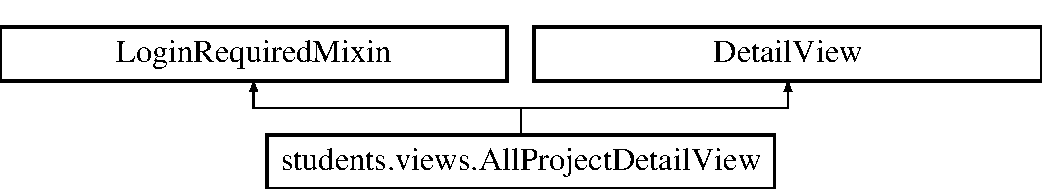
\includegraphics[height=2.000000cm]{classstudents_1_1views_1_1_all_project_detail_view}
\end{center}
\end{figure}
\subsection*{Public Member Functions}
\begin{DoxyCompactItemize}
\item 
def \hyperlink{classstudents_1_1views_1_1_all_project_detail_view_ab4579ea6b73991a980aaf7d0d7e373e8}{dispatch}
\item 
def \hyperlink{classstudents_1_1views_1_1_all_project_detail_view_a501ce935af27d501442b472b27c71bda}{get\-\_\-object}
\item 
def \hyperlink{classstudents_1_1views_1_1_all_project_detail_view_ae9bf8cd5bb54a5b7071c273aaf2cae53}{get\-\_\-context\-\_\-data}
\end{DoxyCompactItemize}
\subsection*{Static Public Attributes}
\begin{DoxyCompactItemize}
\item 
string \hyperlink{classstudents_1_1views_1_1_all_project_detail_view_a6455b90d3855458abb8d369c26322c29}{template\-\_\-name} = \char`\"{}all\-\_\-project\-\_\-detail\-\_\-view.\-html\char`\"{}
\item 
string \hyperlink{classstudents_1_1views_1_1_all_project_detail_view_a58608f95af2ecd53269734a03d805f3f}{login\-\_\-url} = \char`\"{}/students/login/\char`\"{}
\item 
\hyperlink{classstudents_1_1views_1_1_all_project_detail_view_a4cfc7df6cba375623235cb90098767d9}{model} = Project
\end{DoxyCompactItemize}


\subsection{Member Function Documentation}
\hypertarget{classstudents_1_1views_1_1_all_project_detail_view_ab4579ea6b73991a980aaf7d0d7e373e8}{\index{students\-::views\-::\-All\-Project\-Detail\-View@{students\-::views\-::\-All\-Project\-Detail\-View}!dispatch@{dispatch}}
\index{dispatch@{dispatch}!students::views::AllProjectDetailView@{students\-::views\-::\-All\-Project\-Detail\-View}}
\subsubsection[{dispatch}]{\setlength{\rightskip}{0pt plus 5cm}def students.\-views.\-All\-Project\-Detail\-View.\-dispatch (
\begin{DoxyParamCaption}
\item[{}]{self, }
\item[{}]{request, }
\item[{}]{args, }
\item[{}]{kwargs}
\end{DoxyParamCaption}
)}}\label{classstudents_1_1views_1_1_all_project_detail_view_ab4579ea6b73991a980aaf7d0d7e373e8}
\hypertarget{classstudents_1_1views_1_1_all_project_detail_view_ae9bf8cd5bb54a5b7071c273aaf2cae53}{\index{students\-::views\-::\-All\-Project\-Detail\-View@{students\-::views\-::\-All\-Project\-Detail\-View}!get\-\_\-context\-\_\-data@{get\-\_\-context\-\_\-data}}
\index{get\-\_\-context\-\_\-data@{get\-\_\-context\-\_\-data}!students::views::AllProjectDetailView@{students\-::views\-::\-All\-Project\-Detail\-View}}
\subsubsection[{get\-\_\-context\-\_\-data}]{\setlength{\rightskip}{0pt plus 5cm}def students.\-views.\-All\-Project\-Detail\-View.\-get\-\_\-context\-\_\-data (
\begin{DoxyParamCaption}
\item[{}]{self, }
\item[{}]{kwargs}
\end{DoxyParamCaption}
)}}\label{classstudents_1_1views_1_1_all_project_detail_view_ae9bf8cd5bb54a5b7071c273aaf2cae53}
\hypertarget{classstudents_1_1views_1_1_all_project_detail_view_a501ce935af27d501442b472b27c71bda}{\index{students\-::views\-::\-All\-Project\-Detail\-View@{students\-::views\-::\-All\-Project\-Detail\-View}!get\-\_\-object@{get\-\_\-object}}
\index{get\-\_\-object@{get\-\_\-object}!students::views::AllProjectDetailView@{students\-::views\-::\-All\-Project\-Detail\-View}}
\subsubsection[{get\-\_\-object}]{\setlength{\rightskip}{0pt plus 5cm}def students.\-views.\-All\-Project\-Detail\-View.\-get\-\_\-object (
\begin{DoxyParamCaption}
\item[{}]{self, }
\item[{}]{queryset = {\ttfamily None}}
\end{DoxyParamCaption}
)}}\label{classstudents_1_1views_1_1_all_project_detail_view_a501ce935af27d501442b472b27c71bda}


\subsection{Member Data Documentation}
\hypertarget{classstudents_1_1views_1_1_all_project_detail_view_a58608f95af2ecd53269734a03d805f3f}{\index{students\-::views\-::\-All\-Project\-Detail\-View@{students\-::views\-::\-All\-Project\-Detail\-View}!login\-\_\-url@{login\-\_\-url}}
\index{login\-\_\-url@{login\-\_\-url}!students::views::AllProjectDetailView@{students\-::views\-::\-All\-Project\-Detail\-View}}
\subsubsection[{login\-\_\-url}]{\setlength{\rightskip}{0pt plus 5cm}string students.\-views.\-All\-Project\-Detail\-View.\-login\-\_\-url = \char`\"{}/students/login/\char`\"{}\hspace{0.3cm}{\ttfamily [static]}}}\label{classstudents_1_1views_1_1_all_project_detail_view_a58608f95af2ecd53269734a03d805f3f}
\hypertarget{classstudents_1_1views_1_1_all_project_detail_view_a4cfc7df6cba375623235cb90098767d9}{\index{students\-::views\-::\-All\-Project\-Detail\-View@{students\-::views\-::\-All\-Project\-Detail\-View}!model@{model}}
\index{model@{model}!students::views::AllProjectDetailView@{students\-::views\-::\-All\-Project\-Detail\-View}}
\subsubsection[{model}]{\setlength{\rightskip}{0pt plus 5cm}students.\-views.\-All\-Project\-Detail\-View.\-model = Project\hspace{0.3cm}{\ttfamily [static]}}}\label{classstudents_1_1views_1_1_all_project_detail_view_a4cfc7df6cba375623235cb90098767d9}
\hypertarget{classstudents_1_1views_1_1_all_project_detail_view_a6455b90d3855458abb8d369c26322c29}{\index{students\-::views\-::\-All\-Project\-Detail\-View@{students\-::views\-::\-All\-Project\-Detail\-View}!template\-\_\-name@{template\-\_\-name}}
\index{template\-\_\-name@{template\-\_\-name}!students::views::AllProjectDetailView@{students\-::views\-::\-All\-Project\-Detail\-View}}
\subsubsection[{template\-\_\-name}]{\setlength{\rightskip}{0pt plus 5cm}string students.\-views.\-All\-Project\-Detail\-View.\-template\-\_\-name = \char`\"{}all\-\_\-project\-\_\-detail\-\_\-view.\-html\char`\"{}\hspace{0.3cm}{\ttfamily [static]}}}\label{classstudents_1_1views_1_1_all_project_detail_view_a6455b90d3855458abb8d369c26322c29}


The documentation for this class was generated from the following file\-:\begin{DoxyCompactItemize}
\item 
leapkit/students/\hyperlink{views_8py}{views.\-py}\end{DoxyCompactItemize}

\hypertarget{classstudents_1_1views_1_1_change_password_view}{\section{students.\-views.\-Change\-Password\-View Class Reference}
\label{classstudents_1_1views_1_1_change_password_view}\index{students.\-views.\-Change\-Password\-View@{students.\-views.\-Change\-Password\-View}}
}
Inheritance diagram for students.\-views.\-Change\-Password\-View\-:\begin{figure}[H]
\begin{center}
\leavevmode
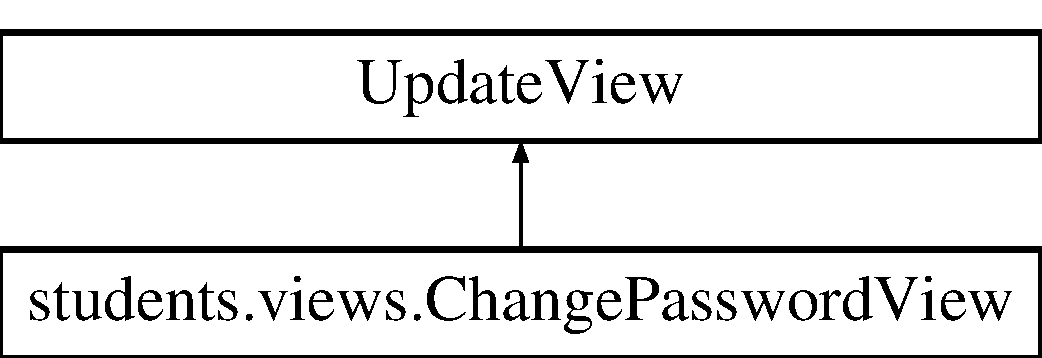
\includegraphics[height=2.000000cm]{classstudents_1_1views_1_1_change_password_view}
\end{center}
\end{figure}
\subsection*{Public Member Functions}
\begin{DoxyCompactItemize}
\item 
def \hyperlink{classstudents_1_1views_1_1_change_password_view_a4ca0c857f594e8521613d3ef0734a96c}{form\-\_\-valid}
\end{DoxyCompactItemize}
\subsection*{Static Public Attributes}
\begin{DoxyCompactItemize}
\item 
string \hyperlink{classstudents_1_1views_1_1_change_password_view_adf894d4b12b423868347159314d99c8f}{template\-\_\-name} = \char`\"{}change\-\_\-student\-\_\-password.\-html\char`\"{}
\item 
\hyperlink{classstudents_1_1views_1_1_change_password_view_ae00b0734c96a70c9b26cccd21de43835}{model} = User
\item 
\hyperlink{classstudents_1_1views_1_1_change_password_view_aa214f4113b8b57922af5caeba0cc0309}{form\-\_\-class} = Change\-User\-Password
\end{DoxyCompactItemize}


\subsection{Member Function Documentation}
\hypertarget{classstudents_1_1views_1_1_change_password_view_a4ca0c857f594e8521613d3ef0734a96c}{\index{students\-::views\-::\-Change\-Password\-View@{students\-::views\-::\-Change\-Password\-View}!form\-\_\-valid@{form\-\_\-valid}}
\index{form\-\_\-valid@{form\-\_\-valid}!students::views::ChangePasswordView@{students\-::views\-::\-Change\-Password\-View}}
\subsubsection[{form\-\_\-valid}]{\setlength{\rightskip}{0pt plus 5cm}def students.\-views.\-Change\-Password\-View.\-form\-\_\-valid (
\begin{DoxyParamCaption}
\item[{}]{self, }
\item[{}]{form}
\end{DoxyParamCaption}
)}}\label{classstudents_1_1views_1_1_change_password_view_a4ca0c857f594e8521613d3ef0734a96c}


\subsection{Member Data Documentation}
\hypertarget{classstudents_1_1views_1_1_change_password_view_aa214f4113b8b57922af5caeba0cc0309}{\index{students\-::views\-::\-Change\-Password\-View@{students\-::views\-::\-Change\-Password\-View}!form\-\_\-class@{form\-\_\-class}}
\index{form\-\_\-class@{form\-\_\-class}!students::views::ChangePasswordView@{students\-::views\-::\-Change\-Password\-View}}
\subsubsection[{form\-\_\-class}]{\setlength{\rightskip}{0pt plus 5cm}students.\-views.\-Change\-Password\-View.\-form\-\_\-class = Change\-User\-Password\hspace{0.3cm}{\ttfamily [static]}}}\label{classstudents_1_1views_1_1_change_password_view_aa214f4113b8b57922af5caeba0cc0309}
\hypertarget{classstudents_1_1views_1_1_change_password_view_ae00b0734c96a70c9b26cccd21de43835}{\index{students\-::views\-::\-Change\-Password\-View@{students\-::views\-::\-Change\-Password\-View}!model@{model}}
\index{model@{model}!students::views::ChangePasswordView@{students\-::views\-::\-Change\-Password\-View}}
\subsubsection[{model}]{\setlength{\rightskip}{0pt plus 5cm}students.\-views.\-Change\-Password\-View.\-model = User\hspace{0.3cm}{\ttfamily [static]}}}\label{classstudents_1_1views_1_1_change_password_view_ae00b0734c96a70c9b26cccd21de43835}
\hypertarget{classstudents_1_1views_1_1_change_password_view_adf894d4b12b423868347159314d99c8f}{\index{students\-::views\-::\-Change\-Password\-View@{students\-::views\-::\-Change\-Password\-View}!template\-\_\-name@{template\-\_\-name}}
\index{template\-\_\-name@{template\-\_\-name}!students::views::ChangePasswordView@{students\-::views\-::\-Change\-Password\-View}}
\subsubsection[{template\-\_\-name}]{\setlength{\rightskip}{0pt plus 5cm}string students.\-views.\-Change\-Password\-View.\-template\-\_\-name = \char`\"{}change\-\_\-student\-\_\-password.\-html\char`\"{}\hspace{0.3cm}{\ttfamily [static]}}}\label{classstudents_1_1views_1_1_change_password_view_adf894d4b12b423868347159314d99c8f}


The documentation for this class was generated from the following file\-:\begin{DoxyCompactItemize}
\item 
leapkit/students/\hyperlink{views_8py}{views.\-py}\end{DoxyCompactItemize}

\hypertarget{classstudents_1_1forms_1_1_change_user_password}{\section{students.\-forms.\-Change\-User\-Password Class Reference}
\label{classstudents_1_1forms_1_1_change_user_password}\index{students.\-forms.\-Change\-User\-Password@{students.\-forms.\-Change\-User\-Password}}
}
Inheritance diagram for students.\-forms.\-Change\-User\-Password\-:\begin{figure}[H]
\begin{center}
\leavevmode
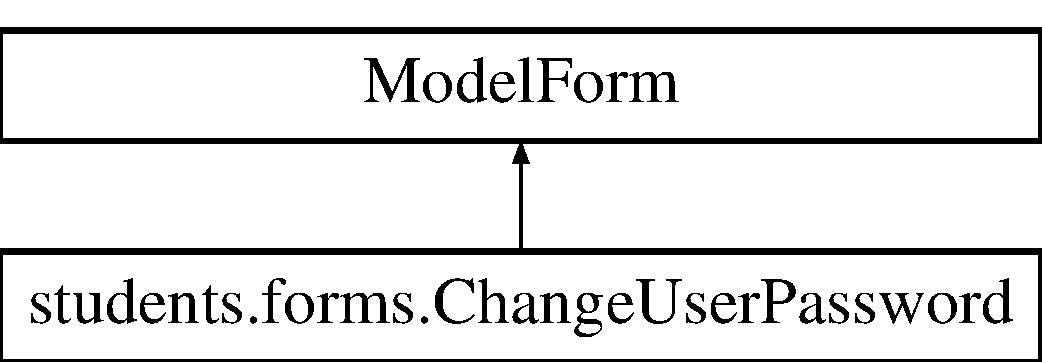
\includegraphics[height=2.000000cm]{classstudents_1_1forms_1_1_change_user_password}
\end{center}
\end{figure}
\subsection*{Classes}
\begin{DoxyCompactItemize}
\item 
class \hyperlink{classstudents_1_1forms_1_1_change_user_password_1_1_meta}{Meta}
\end{DoxyCompactItemize}
\subsection*{Public Member Functions}
\begin{DoxyCompactItemize}
\item 
def \hyperlink{classstudents_1_1forms_1_1_change_user_password_a400af3a93c05d7d6e3ea1158f31bd7f3}{\-\_\-\-\_\-init\-\_\-\-\_\-}
\item 
def \hyperlink{classstudents_1_1forms_1_1_change_user_password_a9e5064d034ff778807af126d1356516e}{clean\-\_\-old\-\_\-password}
\item 
def \hyperlink{classstudents_1_1forms_1_1_change_user_password_aa6903c9f9f85107a18b9b3ce687df81b}{clean\-\_\-password2}
\item 
def \hyperlink{classstudents_1_1forms_1_1_change_user_password_a3c5e1bccb71fbac3c774d759ede60dfb}{save}
\end{DoxyCompactItemize}
\subsection*{Public Attributes}
\begin{DoxyCompactItemize}
\item 
\hyperlink{classstudents_1_1forms_1_1_change_user_password_a3a93705cd4e07df9ffc88668c9c4197d}{helper}
\end{DoxyCompactItemize}
\subsection*{Static Public Attributes}
\begin{DoxyCompactItemize}
\item 
tuple \hyperlink{classstudents_1_1forms_1_1_change_user_password_ad1755c0b3431fb3e1921af9569292001}{old\-\_\-password} = forms.\-Char\-Field(required=True, widget=forms.\-Password\-Input())
\item 
tuple \hyperlink{classstudents_1_1forms_1_1_change_user_password_a9c5c21d107754a8aa78c93bcf9d1071c}{password1} = forms.\-Char\-Field(required=True, widget=forms.\-Password\-Input())
\item 
tuple \hyperlink{classstudents_1_1forms_1_1_change_user_password_a964e8b5309d12749528691a264d9266e}{password2} = forms.\-Char\-Field(required=True, widget=forms.\-Password\-Input())
\end{DoxyCompactItemize}


\subsection{Constructor \& Destructor Documentation}
\hypertarget{classstudents_1_1forms_1_1_change_user_password_a400af3a93c05d7d6e3ea1158f31bd7f3}{\index{students\-::forms\-::\-Change\-User\-Password@{students\-::forms\-::\-Change\-User\-Password}!\-\_\-\-\_\-init\-\_\-\-\_\-@{\-\_\-\-\_\-init\-\_\-\-\_\-}}
\index{\-\_\-\-\_\-init\-\_\-\-\_\-@{\-\_\-\-\_\-init\-\_\-\-\_\-}!students::forms::ChangeUserPassword@{students\-::forms\-::\-Change\-User\-Password}}
\subsubsection[{\-\_\-\-\_\-init\-\_\-\-\_\-}]{\setlength{\rightskip}{0pt plus 5cm}def students.\-forms.\-Change\-User\-Password.\-\_\-\-\_\-init\-\_\-\-\_\- (
\begin{DoxyParamCaption}
\item[{}]{self, }
\item[{}]{args, }
\item[{}]{kwargs}
\end{DoxyParamCaption}
)}}\label{classstudents_1_1forms_1_1_change_user_password_a400af3a93c05d7d6e3ea1158f31bd7f3}


\subsection{Member Function Documentation}
\hypertarget{classstudents_1_1forms_1_1_change_user_password_a9e5064d034ff778807af126d1356516e}{\index{students\-::forms\-::\-Change\-User\-Password@{students\-::forms\-::\-Change\-User\-Password}!clean\-\_\-old\-\_\-password@{clean\-\_\-old\-\_\-password}}
\index{clean\-\_\-old\-\_\-password@{clean\-\_\-old\-\_\-password}!students::forms::ChangeUserPassword@{students\-::forms\-::\-Change\-User\-Password}}
\subsubsection[{clean\-\_\-old\-\_\-password}]{\setlength{\rightskip}{0pt plus 5cm}def students.\-forms.\-Change\-User\-Password.\-clean\-\_\-old\-\_\-password (
\begin{DoxyParamCaption}
\item[{}]{self}
\end{DoxyParamCaption}
)}}\label{classstudents_1_1forms_1_1_change_user_password_a9e5064d034ff778807af126d1356516e}
\hypertarget{classstudents_1_1forms_1_1_change_user_password_aa6903c9f9f85107a18b9b3ce687df81b}{\index{students\-::forms\-::\-Change\-User\-Password@{students\-::forms\-::\-Change\-User\-Password}!clean\-\_\-password2@{clean\-\_\-password2}}
\index{clean\-\_\-password2@{clean\-\_\-password2}!students::forms::ChangeUserPassword@{students\-::forms\-::\-Change\-User\-Password}}
\subsubsection[{clean\-\_\-password2}]{\setlength{\rightskip}{0pt plus 5cm}def students.\-forms.\-Change\-User\-Password.\-clean\-\_\-password2 (
\begin{DoxyParamCaption}
\item[{}]{self}
\end{DoxyParamCaption}
)}}\label{classstudents_1_1forms_1_1_change_user_password_aa6903c9f9f85107a18b9b3ce687df81b}
\hypertarget{classstudents_1_1forms_1_1_change_user_password_a3c5e1bccb71fbac3c774d759ede60dfb}{\index{students\-::forms\-::\-Change\-User\-Password@{students\-::forms\-::\-Change\-User\-Password}!save@{save}}
\index{save@{save}!students::forms::ChangeUserPassword@{students\-::forms\-::\-Change\-User\-Password}}
\subsubsection[{save}]{\setlength{\rightskip}{0pt plus 5cm}def students.\-forms.\-Change\-User\-Password.\-save (
\begin{DoxyParamCaption}
\item[{}]{self, }
\item[{}]{commit = {\ttfamily True}}
\end{DoxyParamCaption}
)}}\label{classstudents_1_1forms_1_1_change_user_password_a3c5e1bccb71fbac3c774d759ede60dfb}


\subsection{Member Data Documentation}
\hypertarget{classstudents_1_1forms_1_1_change_user_password_a3a93705cd4e07df9ffc88668c9c4197d}{\index{students\-::forms\-::\-Change\-User\-Password@{students\-::forms\-::\-Change\-User\-Password}!helper@{helper}}
\index{helper@{helper}!students::forms::ChangeUserPassword@{students\-::forms\-::\-Change\-User\-Password}}
\subsubsection[{helper}]{\setlength{\rightskip}{0pt plus 5cm}students.\-forms.\-Change\-User\-Password.\-helper}}\label{classstudents_1_1forms_1_1_change_user_password_a3a93705cd4e07df9ffc88668c9c4197d}
\hypertarget{classstudents_1_1forms_1_1_change_user_password_ad1755c0b3431fb3e1921af9569292001}{\index{students\-::forms\-::\-Change\-User\-Password@{students\-::forms\-::\-Change\-User\-Password}!old\-\_\-password@{old\-\_\-password}}
\index{old\-\_\-password@{old\-\_\-password}!students::forms::ChangeUserPassword@{students\-::forms\-::\-Change\-User\-Password}}
\subsubsection[{old\-\_\-password}]{\setlength{\rightskip}{0pt plus 5cm}tuple students.\-forms.\-Change\-User\-Password.\-old\-\_\-password = forms.\-Char\-Field(required=True, widget=forms.\-Password\-Input())\hspace{0.3cm}{\ttfamily [static]}}}\label{classstudents_1_1forms_1_1_change_user_password_ad1755c0b3431fb3e1921af9569292001}
\hypertarget{classstudents_1_1forms_1_1_change_user_password_a9c5c21d107754a8aa78c93bcf9d1071c}{\index{students\-::forms\-::\-Change\-User\-Password@{students\-::forms\-::\-Change\-User\-Password}!password1@{password1}}
\index{password1@{password1}!students::forms::ChangeUserPassword@{students\-::forms\-::\-Change\-User\-Password}}
\subsubsection[{password1}]{\setlength{\rightskip}{0pt plus 5cm}tuple students.\-forms.\-Change\-User\-Password.\-password1 = forms.\-Char\-Field(required=True, widget=forms.\-Password\-Input())\hspace{0.3cm}{\ttfamily [static]}}}\label{classstudents_1_1forms_1_1_change_user_password_a9c5c21d107754a8aa78c93bcf9d1071c}
\hypertarget{classstudents_1_1forms_1_1_change_user_password_a964e8b5309d12749528691a264d9266e}{\index{students\-::forms\-::\-Change\-User\-Password@{students\-::forms\-::\-Change\-User\-Password}!password2@{password2}}
\index{password2@{password2}!students::forms::ChangeUserPassword@{students\-::forms\-::\-Change\-User\-Password}}
\subsubsection[{password2}]{\setlength{\rightskip}{0pt plus 5cm}tuple students.\-forms.\-Change\-User\-Password.\-password2 = forms.\-Char\-Field(required=True, widget=forms.\-Password\-Input())\hspace{0.3cm}{\ttfamily [static]}}}\label{classstudents_1_1forms_1_1_change_user_password_a964e8b5309d12749528691a264d9266e}


The documentation for this class was generated from the following file\-:\begin{DoxyCompactItemize}
\item 
leapkit/students/\hyperlink{forms_8py}{forms.\-py}\end{DoxyCompactItemize}

\hypertarget{classstudents_1_1models_1_1_course}{\section{students.\-models.\-Course Class Reference}
\label{classstudents_1_1models_1_1_course}\index{students.\-models.\-Course@{students.\-models.\-Course}}
}
Inheritance diagram for students.\-models.\-Course\-:\begin{figure}[H]
\begin{center}
\leavevmode
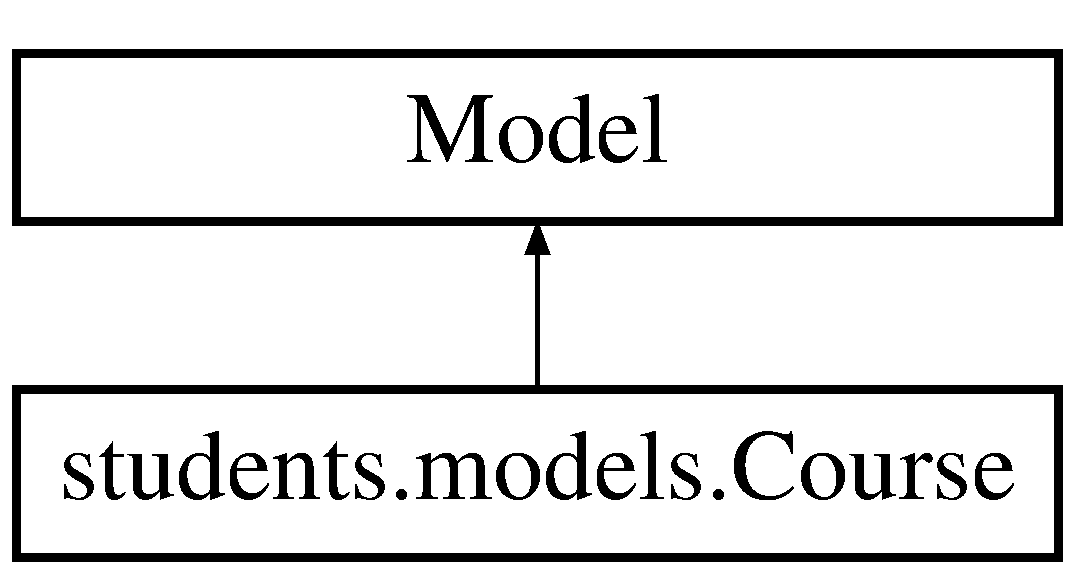
\includegraphics[height=2.000000cm]{classstudents_1_1models_1_1_course}
\end{center}
\end{figure}
\subsection*{Public Member Functions}
\begin{DoxyCompactItemize}
\item 
def \hyperlink{classstudents_1_1models_1_1_course_afcde6983ecb364eb3d26811950f531b0}{\-\_\-\-\_\-unicode\-\_\-\-\_\-}
\item 
def \hyperlink{classstudents_1_1models_1_1_course_afd219fece1d92c93deb18841782d6a16}{get\-\_\-course}
\end{DoxyCompactItemize}
\subsection*{Static Public Attributes}
\begin{DoxyCompactItemize}
\item 
tuple \hyperlink{classstudents_1_1models_1_1_course_a6167f80718f9a71b41abba99105a079c}{name} = models.\-Char\-Field(max\-\_\-length = 81)
\item 
tuple \hyperlink{classstudents_1_1models_1_1_course_aadeceab75e5b99ede00f30b2f56da749}{profile} = models.\-Foreign\-Key(\hyperlink{classstudents_1_1models_1_1_linked_in_profile}{Linked\-In\-Profile})
\end{DoxyCompactItemize}


\subsection{Detailed Description}
\begin{DoxyVerb}Model that represents a course on LinkedIn.
\end{DoxyVerb}
 

\subsection{Member Function Documentation}
\hypertarget{classstudents_1_1models_1_1_course_afcde6983ecb364eb3d26811950f531b0}{\index{students\-::models\-::\-Course@{students\-::models\-::\-Course}!\-\_\-\-\_\-unicode\-\_\-\-\_\-@{\-\_\-\-\_\-unicode\-\_\-\-\_\-}}
\index{\-\_\-\-\_\-unicode\-\_\-\-\_\-@{\-\_\-\-\_\-unicode\-\_\-\-\_\-}!students::models::Course@{students\-::models\-::\-Course}}
\subsubsection[{\-\_\-\-\_\-unicode\-\_\-\-\_\-}]{\setlength{\rightskip}{0pt plus 5cm}def students.\-models.\-Course.\-\_\-\-\_\-unicode\-\_\-\-\_\- (
\begin{DoxyParamCaption}
\item[{}]{self}
\end{DoxyParamCaption}
)}}\label{classstudents_1_1models_1_1_course_afcde6983ecb364eb3d26811950f531b0}
\hypertarget{classstudents_1_1models_1_1_course_afd219fece1d92c93deb18841782d6a16}{\index{students\-::models\-::\-Course@{students\-::models\-::\-Course}!get\-\_\-course@{get\-\_\-course}}
\index{get\-\_\-course@{get\-\_\-course}!students::models::Course@{students\-::models\-::\-Course}}
\subsubsection[{get\-\_\-course}]{\setlength{\rightskip}{0pt plus 5cm}def students.\-models.\-Course.\-get\-\_\-course (
\begin{DoxyParamCaption}
\item[{}]{self}
\end{DoxyParamCaption}
)}}\label{classstudents_1_1models_1_1_course_afd219fece1d92c93deb18841782d6a16}


\subsection{Member Data Documentation}
\hypertarget{classstudents_1_1models_1_1_course_a6167f80718f9a71b41abba99105a079c}{\index{students\-::models\-::\-Course@{students\-::models\-::\-Course}!name@{name}}
\index{name@{name}!students::models::Course@{students\-::models\-::\-Course}}
\subsubsection[{name}]{\setlength{\rightskip}{0pt plus 5cm}tuple students.\-models.\-Course.\-name = models.\-Char\-Field(max\-\_\-length = 81)\hspace{0.3cm}{\ttfamily [static]}}}\label{classstudents_1_1models_1_1_course_a6167f80718f9a71b41abba99105a079c}
\hypertarget{classstudents_1_1models_1_1_course_aadeceab75e5b99ede00f30b2f56da749}{\index{students\-::models\-::\-Course@{students\-::models\-::\-Course}!profile@{profile}}
\index{profile@{profile}!students::models::Course@{students\-::models\-::\-Course}}
\subsubsection[{profile}]{\setlength{\rightskip}{0pt plus 5cm}tuple students.\-models.\-Course.\-profile = models.\-Foreign\-Key({\bf Linked\-In\-Profile})\hspace{0.3cm}{\ttfamily [static]}}}\label{classstudents_1_1models_1_1_course_aadeceab75e5b99ede00f30b2f56da749}


The documentation for this class was generated from the following file\-:\begin{DoxyCompactItemize}
\item 
leapkit/students/\hyperlink{models_8py}{models.\-py}\end{DoxyCompactItemize}

\hypertarget{classstudents_1_1linkedin__converter_1_1_course}{\section{students.\-linkedin\-\_\-converter.\-Course Class Reference}
\label{classstudents_1_1linkedin__converter_1_1_course}\index{students.\-linkedin\-\_\-converter.\-Course@{students.\-linkedin\-\_\-converter.\-Course}}
}
Inheritance diagram for students.\-linkedin\-\_\-converter.\-Course\-:\begin{figure}[H]
\begin{center}
\leavevmode
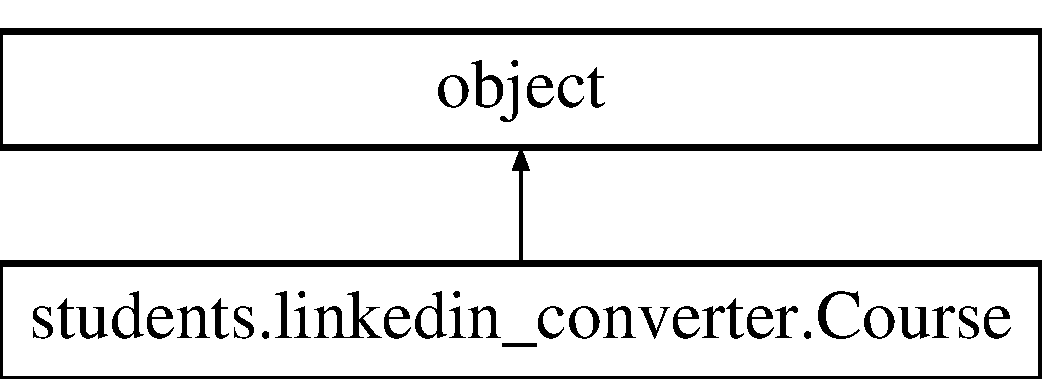
\includegraphics[height=2.000000cm]{classstudents_1_1linkedin__converter_1_1_course}
\end{center}
\end{figure}
\subsection*{Static Public Attributes}
\begin{DoxyCompactItemize}
\item 
string \hyperlink{classstudents_1_1linkedin__converter_1_1_course_a61b6dbcb8128298f44fafc413667c418}{cid} = \char`\"{}\char`\"{}
\item 
string \hyperlink{classstudents_1_1linkedin__converter_1_1_course_a086c26e2a7267f59ebf1ed12aa03344c}{name} = \char`\"{}\char`\"{}
\end{DoxyCompactItemize}


\subsection{Detailed Description}
\begin{DoxyVerb}A Course is used to hold what courses a person has completed.\end{DoxyVerb}
\begin{DoxyVerb}Constructor that initiates all the basic course values\end{DoxyVerb}
 

\subsection{Member Data Documentation}
\hypertarget{classstudents_1_1linkedin__converter_1_1_course_a61b6dbcb8128298f44fafc413667c418}{\index{students\-::linkedin\-\_\-converter\-::\-Course@{students\-::linkedin\-\_\-converter\-::\-Course}!cid@{cid}}
\index{cid@{cid}!students::linkedin_converter::Course@{students\-::linkedin\-\_\-converter\-::\-Course}}
\subsubsection[{cid}]{\setlength{\rightskip}{0pt plus 5cm}string students.\-linkedin\-\_\-converter.\-Course.\-cid = \char`\"{}\char`\"{}\hspace{0.3cm}{\ttfamily [static]}}}\label{classstudents_1_1linkedin__converter_1_1_course_a61b6dbcb8128298f44fafc413667c418}
\hypertarget{classstudents_1_1linkedin__converter_1_1_course_a086c26e2a7267f59ebf1ed12aa03344c}{\index{students\-::linkedin\-\_\-converter\-::\-Course@{students\-::linkedin\-\_\-converter\-::\-Course}!name@{name}}
\index{name@{name}!students::linkedin_converter::Course@{students\-::linkedin\-\_\-converter\-::\-Course}}
\subsubsection[{name}]{\setlength{\rightskip}{0pt plus 5cm}string students.\-linkedin\-\_\-converter.\-Course.\-name = \char`\"{}\char`\"{}\hspace{0.3cm}{\ttfamily [static]}}}\label{classstudents_1_1linkedin__converter_1_1_course_a086c26e2a7267f59ebf1ed12aa03344c}


The documentation for this class was generated from the following file\-:\begin{DoxyCompactItemize}
\item 
leapkit/students/\hyperlink{linkedin__converter_8py}{linkedin\-\_\-converter.\-py}\end{DoxyCompactItemize}

\hypertarget{classstudents_1_1admin_1_1_course_admin}{\section{students.\-admin.\-Course\-Admin Class Reference}
\label{classstudents_1_1admin_1_1_course_admin}\index{students.\-admin.\-Course\-Admin@{students.\-admin.\-Course\-Admin}}
}
Inheritance diagram for students.\-admin.\-Course\-Admin\-:\begin{figure}[H]
\begin{center}
\leavevmode
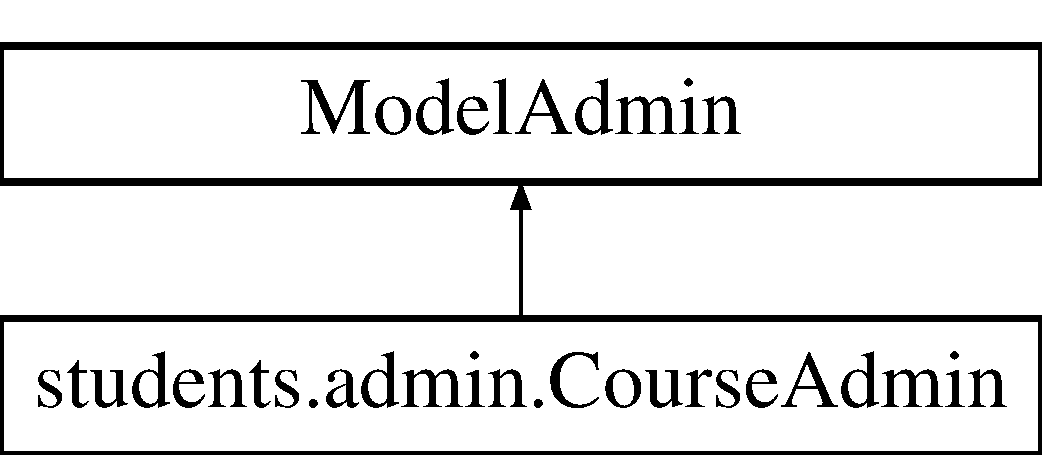
\includegraphics[height=2.000000cm]{classstudents_1_1admin_1_1_course_admin}
\end{center}
\end{figure}
\subsection*{Static Public Attributes}
\begin{DoxyCompactItemize}
\item 
list \hyperlink{classstudents_1_1admin_1_1_course_admin_a2d298dca126bc069d952e3b203c7ff9a}{fieldsets} = \mbox{[}(None, \{'fields' \-: \mbox{[}'name', 'profile'\mbox{]}\}),\mbox{]}
\item 
tuple \hyperlink{classstudents_1_1admin_1_1_course_admin_a2875b817163ff5678d1325780528df79}{list\-\_\-display} = ('name', 'profile')
\item 
list \hyperlink{classstudents_1_1admin_1_1_course_admin_aafd6b90008831c42064c629a6a6ff294}{search\-\_\-fields} = \mbox{[}'name', 'profile'\mbox{]}
\end{DoxyCompactItemize}


\subsection{Member Data Documentation}
\hypertarget{classstudents_1_1admin_1_1_course_admin_a2d298dca126bc069d952e3b203c7ff9a}{\index{students\-::admin\-::\-Course\-Admin@{students\-::admin\-::\-Course\-Admin}!fieldsets@{fieldsets}}
\index{fieldsets@{fieldsets}!students::admin::CourseAdmin@{students\-::admin\-::\-Course\-Admin}}
\subsubsection[{fieldsets}]{\setlength{\rightskip}{0pt plus 5cm}list students.\-admin.\-Course\-Admin.\-fieldsets = \mbox{[}(None, \{'fields' \-: \mbox{[}'name', 'profile'\mbox{]}\}),\mbox{]}\hspace{0.3cm}{\ttfamily [static]}}}\label{classstudents_1_1admin_1_1_course_admin_a2d298dca126bc069d952e3b203c7ff9a}
\hypertarget{classstudents_1_1admin_1_1_course_admin_a2875b817163ff5678d1325780528df79}{\index{students\-::admin\-::\-Course\-Admin@{students\-::admin\-::\-Course\-Admin}!list\-\_\-display@{list\-\_\-display}}
\index{list\-\_\-display@{list\-\_\-display}!students::admin::CourseAdmin@{students\-::admin\-::\-Course\-Admin}}
\subsubsection[{list\-\_\-display}]{\setlength{\rightskip}{0pt plus 5cm}tuple students.\-admin.\-Course\-Admin.\-list\-\_\-display = ('name', 'profile')\hspace{0.3cm}{\ttfamily [static]}}}\label{classstudents_1_1admin_1_1_course_admin_a2875b817163ff5678d1325780528df79}
\hypertarget{classstudents_1_1admin_1_1_course_admin_aafd6b90008831c42064c629a6a6ff294}{\index{students\-::admin\-::\-Course\-Admin@{students\-::admin\-::\-Course\-Admin}!search\-\_\-fields@{search\-\_\-fields}}
\index{search\-\_\-fields@{search\-\_\-fields}!students::admin::CourseAdmin@{students\-::admin\-::\-Course\-Admin}}
\subsubsection[{search\-\_\-fields}]{\setlength{\rightskip}{0pt plus 5cm}list students.\-admin.\-Course\-Admin.\-search\-\_\-fields = \mbox{[}'name', 'profile'\mbox{]}\hspace{0.3cm}{\ttfamily [static]}}}\label{classstudents_1_1admin_1_1_course_admin_aafd6b90008831c42064c629a6a6ff294}


The documentation for this class was generated from the following file\-:\begin{DoxyCompactItemize}
\item 
leapkit/students/\hyperlink{admin_8py}{admin.\-py}\end{DoxyCompactItemize}

\hypertarget{classstudents_1_1models_1_1_education}{\section{students.\-models.\-Education Class Reference}
\label{classstudents_1_1models_1_1_education}\index{students.\-models.\-Education@{students.\-models.\-Education}}
}
Inheritance diagram for students.\-models.\-Education\-:\begin{figure}[H]
\begin{center}
\leavevmode
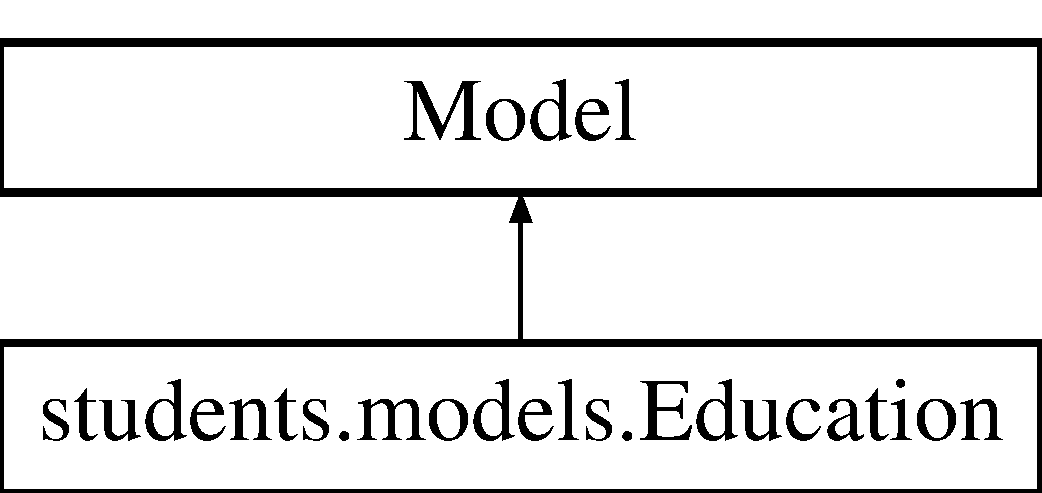
\includegraphics[height=2.000000cm]{classstudents_1_1models_1_1_education}
\end{center}
\end{figure}
\subsection*{Public Member Functions}
\begin{DoxyCompactItemize}
\item 
def \hyperlink{classstudents_1_1models_1_1_education_a359443228da9a61334cc9d640292b2c1}{\-\_\-\-\_\-unicode\-\_\-\-\_\-}
\item 
def \hyperlink{classstudents_1_1models_1_1_education_ac93a74960eafbe9ad36545070e2ee866}{get\-\_\-field\-Of\-Study}
\end{DoxyCompactItemize}
\subsection*{Static Public Attributes}
\begin{DoxyCompactItemize}
\item 
tuple \hyperlink{classstudents_1_1models_1_1_education_adf8328e588ab00fd0dc969f45410965d}{school\-Name} = models.\-Char\-Field(max\-\_\-length=100)
\item 
tuple \hyperlink{classstudents_1_1models_1_1_education_acd4a5b8574fb277183cc459776b58ec9}{field\-Of\-Study} = models.\-Char\-Field(max\-\_\-length=100)
\item 
tuple \hyperlink{classstudents_1_1models_1_1_education_a32495524f30233cc0f398a859edfc239}{degree} = models.\-Char\-Field(max\-\_\-length=100)
\item 
tuple \hyperlink{classstudents_1_1models_1_1_education_a7f96253e2068278fe25499989c8dcdbe}{profile} = models.\-Foreign\-Key(\hyperlink{classstudents_1_1models_1_1_linked_in_profile}{Linked\-In\-Profile})
\end{DoxyCompactItemize}


\subsection{Detailed Description}
\begin{DoxyVerb}Model that represents a education on LinkedIn.
\end{DoxyVerb}
 

\subsection{Member Function Documentation}
\hypertarget{classstudents_1_1models_1_1_education_a359443228da9a61334cc9d640292b2c1}{\index{students\-::models\-::\-Education@{students\-::models\-::\-Education}!\-\_\-\-\_\-unicode\-\_\-\-\_\-@{\-\_\-\-\_\-unicode\-\_\-\-\_\-}}
\index{\-\_\-\-\_\-unicode\-\_\-\-\_\-@{\-\_\-\-\_\-unicode\-\_\-\-\_\-}!students::models::Education@{students\-::models\-::\-Education}}
\subsubsection[{\-\_\-\-\_\-unicode\-\_\-\-\_\-}]{\setlength{\rightskip}{0pt plus 5cm}def students.\-models.\-Education.\-\_\-\-\_\-unicode\-\_\-\-\_\- (
\begin{DoxyParamCaption}
\item[{}]{self}
\end{DoxyParamCaption}
)}}\label{classstudents_1_1models_1_1_education_a359443228da9a61334cc9d640292b2c1}
\hypertarget{classstudents_1_1models_1_1_education_ac93a74960eafbe9ad36545070e2ee866}{\index{students\-::models\-::\-Education@{students\-::models\-::\-Education}!get\-\_\-field\-Of\-Study@{get\-\_\-field\-Of\-Study}}
\index{get\-\_\-field\-Of\-Study@{get\-\_\-field\-Of\-Study}!students::models::Education@{students\-::models\-::\-Education}}
\subsubsection[{get\-\_\-field\-Of\-Study}]{\setlength{\rightskip}{0pt plus 5cm}def students.\-models.\-Education.\-get\-\_\-field\-Of\-Study (
\begin{DoxyParamCaption}
\item[{}]{self}
\end{DoxyParamCaption}
)}}\label{classstudents_1_1models_1_1_education_ac93a74960eafbe9ad36545070e2ee866}


\subsection{Member Data Documentation}
\hypertarget{classstudents_1_1models_1_1_education_a32495524f30233cc0f398a859edfc239}{\index{students\-::models\-::\-Education@{students\-::models\-::\-Education}!degree@{degree}}
\index{degree@{degree}!students::models::Education@{students\-::models\-::\-Education}}
\subsubsection[{degree}]{\setlength{\rightskip}{0pt plus 5cm}tuple students.\-models.\-Education.\-degree = models.\-Char\-Field(max\-\_\-length=100)\hspace{0.3cm}{\ttfamily [static]}}}\label{classstudents_1_1models_1_1_education_a32495524f30233cc0f398a859edfc239}
\hypertarget{classstudents_1_1models_1_1_education_acd4a5b8574fb277183cc459776b58ec9}{\index{students\-::models\-::\-Education@{students\-::models\-::\-Education}!field\-Of\-Study@{field\-Of\-Study}}
\index{field\-Of\-Study@{field\-Of\-Study}!students::models::Education@{students\-::models\-::\-Education}}
\subsubsection[{field\-Of\-Study}]{\setlength{\rightskip}{0pt plus 5cm}tuple students.\-models.\-Education.\-field\-Of\-Study = models.\-Char\-Field(max\-\_\-length=100)\hspace{0.3cm}{\ttfamily [static]}}}\label{classstudents_1_1models_1_1_education_acd4a5b8574fb277183cc459776b58ec9}
\hypertarget{classstudents_1_1models_1_1_education_a7f96253e2068278fe25499989c8dcdbe}{\index{students\-::models\-::\-Education@{students\-::models\-::\-Education}!profile@{profile}}
\index{profile@{profile}!students::models::Education@{students\-::models\-::\-Education}}
\subsubsection[{profile}]{\setlength{\rightskip}{0pt plus 5cm}tuple students.\-models.\-Education.\-profile = models.\-Foreign\-Key({\bf Linked\-In\-Profile})\hspace{0.3cm}{\ttfamily [static]}}}\label{classstudents_1_1models_1_1_education_a7f96253e2068278fe25499989c8dcdbe}
\hypertarget{classstudents_1_1models_1_1_education_adf8328e588ab00fd0dc969f45410965d}{\index{students\-::models\-::\-Education@{students\-::models\-::\-Education}!school\-Name@{school\-Name}}
\index{school\-Name@{school\-Name}!students::models::Education@{students\-::models\-::\-Education}}
\subsubsection[{school\-Name}]{\setlength{\rightskip}{0pt plus 5cm}tuple students.\-models.\-Education.\-school\-Name = models.\-Char\-Field(max\-\_\-length=100)\hspace{0.3cm}{\ttfamily [static]}}}\label{classstudents_1_1models_1_1_education_adf8328e588ab00fd0dc969f45410965d}


The documentation for this class was generated from the following file\-:\begin{DoxyCompactItemize}
\item 
leapkit/students/\hyperlink{models_8py}{models.\-py}\end{DoxyCompactItemize}

\hypertarget{classstudents_1_1linkedin__converter_1_1_education}{\section{students.\-linkedin\-\_\-converter.\-Education Class Reference}
\label{classstudents_1_1linkedin__converter_1_1_education}\index{students.\-linkedin\-\_\-converter.\-Education@{students.\-linkedin\-\_\-converter.\-Education}}
}
Inheritance diagram for students.\-linkedin\-\_\-converter.\-Education\-:\begin{figure}[H]
\begin{center}
\leavevmode
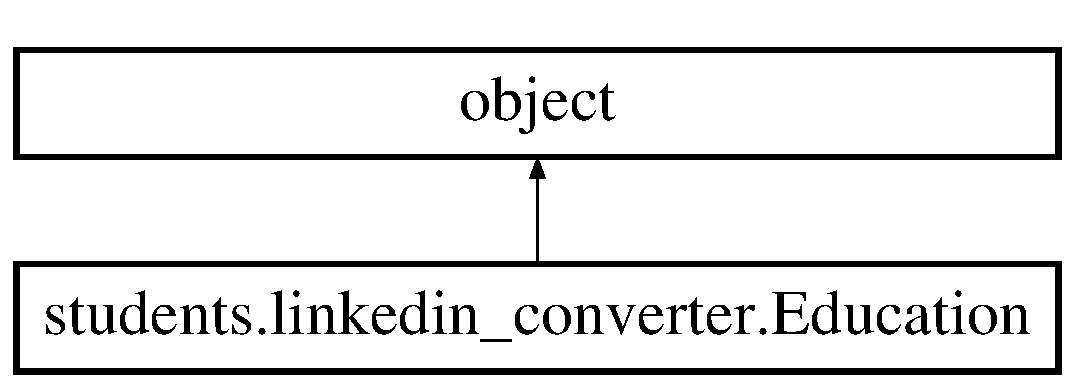
\includegraphics[height=2.000000cm]{classstudents_1_1linkedin__converter_1_1_education}
\end{center}
\end{figure}
\subsection*{Static Public Attributes}
\begin{DoxyCompactItemize}
\item 
string \hyperlink{classstudents_1_1linkedin__converter_1_1_education_a6063bcfc937fd2bff573e9afbbcf3397}{eid} = \char`\"{}\char`\"{}
\item 
string \hyperlink{classstudents_1_1linkedin__converter_1_1_education_afbce23ee5c2c52b61bfa11c8939b4765}{school\-Name} = \char`\"{}\char`\"{}
\item 
string \hyperlink{classstudents_1_1linkedin__converter_1_1_education_ac1ea0d7760168e3bcf6a22cbc77b3009}{field\-Of\-Study} = \char`\"{}\char`\"{}
\item 
string \hyperlink{classstudents_1_1linkedin__converter_1_1_education_ac9f024efe815cfcd3909023f5104a21c}{start\-Date} = \char`\"{}\char`\"{}
\item 
string \hyperlink{classstudents_1_1linkedin__converter_1_1_education_af8ff3553515ad802d83119ec41244172}{end\-Date} = \char`\"{}\char`\"{}
\item 
string \hyperlink{classstudents_1_1linkedin__converter_1_1_education_a95e740f34b15f9f118e5b33d5058bd08}{degree} = \char`\"{}\char`\"{}
\end{DoxyCompactItemize}


\subsection{Detailed Description}
\begin{DoxyVerb}Education hold what educations a person has completed, what degree it
gives and from where it was given.\end{DoxyVerb}
\begin{DoxyVerb}Constructor that initiates all the basic education values\end{DoxyVerb}
 

\subsection{Member Data Documentation}
\hypertarget{classstudents_1_1linkedin__converter_1_1_education_a95e740f34b15f9f118e5b33d5058bd08}{\index{students\-::linkedin\-\_\-converter\-::\-Education@{students\-::linkedin\-\_\-converter\-::\-Education}!degree@{degree}}
\index{degree@{degree}!students::linkedin_converter::Education@{students\-::linkedin\-\_\-converter\-::\-Education}}
\subsubsection[{degree}]{\setlength{\rightskip}{0pt plus 5cm}string students.\-linkedin\-\_\-converter.\-Education.\-degree = \char`\"{}\char`\"{}\hspace{0.3cm}{\ttfamily [static]}}}\label{classstudents_1_1linkedin__converter_1_1_education_a95e740f34b15f9f118e5b33d5058bd08}
\hypertarget{classstudents_1_1linkedin__converter_1_1_education_a6063bcfc937fd2bff573e9afbbcf3397}{\index{students\-::linkedin\-\_\-converter\-::\-Education@{students\-::linkedin\-\_\-converter\-::\-Education}!eid@{eid}}
\index{eid@{eid}!students::linkedin_converter::Education@{students\-::linkedin\-\_\-converter\-::\-Education}}
\subsubsection[{eid}]{\setlength{\rightskip}{0pt plus 5cm}string students.\-linkedin\-\_\-converter.\-Education.\-eid = \char`\"{}\char`\"{}\hspace{0.3cm}{\ttfamily [static]}}}\label{classstudents_1_1linkedin__converter_1_1_education_a6063bcfc937fd2bff573e9afbbcf3397}
\hypertarget{classstudents_1_1linkedin__converter_1_1_education_af8ff3553515ad802d83119ec41244172}{\index{students\-::linkedin\-\_\-converter\-::\-Education@{students\-::linkedin\-\_\-converter\-::\-Education}!end\-Date@{end\-Date}}
\index{end\-Date@{end\-Date}!students::linkedin_converter::Education@{students\-::linkedin\-\_\-converter\-::\-Education}}
\subsubsection[{end\-Date}]{\setlength{\rightskip}{0pt plus 5cm}string students.\-linkedin\-\_\-converter.\-Education.\-end\-Date = \char`\"{}\char`\"{}\hspace{0.3cm}{\ttfamily [static]}}}\label{classstudents_1_1linkedin__converter_1_1_education_af8ff3553515ad802d83119ec41244172}
\hypertarget{classstudents_1_1linkedin__converter_1_1_education_ac1ea0d7760168e3bcf6a22cbc77b3009}{\index{students\-::linkedin\-\_\-converter\-::\-Education@{students\-::linkedin\-\_\-converter\-::\-Education}!field\-Of\-Study@{field\-Of\-Study}}
\index{field\-Of\-Study@{field\-Of\-Study}!students::linkedin_converter::Education@{students\-::linkedin\-\_\-converter\-::\-Education}}
\subsubsection[{field\-Of\-Study}]{\setlength{\rightskip}{0pt plus 5cm}string students.\-linkedin\-\_\-converter.\-Education.\-field\-Of\-Study = \char`\"{}\char`\"{}\hspace{0.3cm}{\ttfamily [static]}}}\label{classstudents_1_1linkedin__converter_1_1_education_ac1ea0d7760168e3bcf6a22cbc77b3009}
\hypertarget{classstudents_1_1linkedin__converter_1_1_education_afbce23ee5c2c52b61bfa11c8939b4765}{\index{students\-::linkedin\-\_\-converter\-::\-Education@{students\-::linkedin\-\_\-converter\-::\-Education}!school\-Name@{school\-Name}}
\index{school\-Name@{school\-Name}!students::linkedin_converter::Education@{students\-::linkedin\-\_\-converter\-::\-Education}}
\subsubsection[{school\-Name}]{\setlength{\rightskip}{0pt plus 5cm}string students.\-linkedin\-\_\-converter.\-Education.\-school\-Name = \char`\"{}\char`\"{}\hspace{0.3cm}{\ttfamily [static]}}}\label{classstudents_1_1linkedin__converter_1_1_education_afbce23ee5c2c52b61bfa11c8939b4765}
\hypertarget{classstudents_1_1linkedin__converter_1_1_education_ac9f024efe815cfcd3909023f5104a21c}{\index{students\-::linkedin\-\_\-converter\-::\-Education@{students\-::linkedin\-\_\-converter\-::\-Education}!start\-Date@{start\-Date}}
\index{start\-Date@{start\-Date}!students::linkedin_converter::Education@{students\-::linkedin\-\_\-converter\-::\-Education}}
\subsubsection[{start\-Date}]{\setlength{\rightskip}{0pt plus 5cm}string students.\-linkedin\-\_\-converter.\-Education.\-start\-Date = \char`\"{}\char`\"{}\hspace{0.3cm}{\ttfamily [static]}}}\label{classstudents_1_1linkedin__converter_1_1_education_ac9f024efe815cfcd3909023f5104a21c}


The documentation for this class was generated from the following file\-:\begin{DoxyCompactItemize}
\item 
leapkit/students/\hyperlink{linkedin__converter_8py}{linkedin\-\_\-converter.\-py}\end{DoxyCompactItemize}

\hypertarget{classstudents_1_1admin_1_1_education_admin}{\section{students.\-admin.\-Education\-Admin Class Reference}
\label{classstudents_1_1admin_1_1_education_admin}\index{students.\-admin.\-Education\-Admin@{students.\-admin.\-Education\-Admin}}
}
Inheritance diagram for students.\-admin.\-Education\-Admin\-:\begin{figure}[H]
\begin{center}
\leavevmode
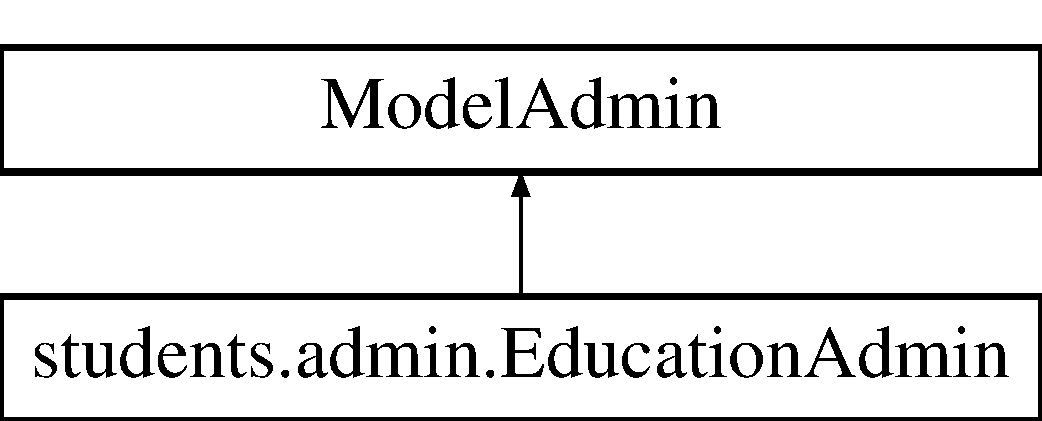
\includegraphics[height=2.000000cm]{classstudents_1_1admin_1_1_education_admin}
\end{center}
\end{figure}
\subsection*{Static Public Attributes}
\begin{DoxyCompactItemize}
\item 
list \hyperlink{classstudents_1_1admin_1_1_education_admin_a67e5ca4edffc907cb58002f86916faf4}{fieldsets}
\item 
tuple \hyperlink{classstudents_1_1admin_1_1_education_admin_a09f7b742c0a5a1e114576ae9529f8e51}{list\-\_\-display} = ('school\-Name', 'field\-Of\-Study', 'degree', 'profile')
\item 
list \hyperlink{classstudents_1_1admin_1_1_education_admin_a7240de856d0b49bae16a0e65804dcefa}{search\-\_\-fields} = \mbox{[}'field\-Of\-Study', 'degree', 'profile'\mbox{]}
\end{DoxyCompactItemize}


\subsection{Member Data Documentation}
\hypertarget{classstudents_1_1admin_1_1_education_admin_a67e5ca4edffc907cb58002f86916faf4}{\index{students\-::admin\-::\-Education\-Admin@{students\-::admin\-::\-Education\-Admin}!fieldsets@{fieldsets}}
\index{fieldsets@{fieldsets}!students::admin::EducationAdmin@{students\-::admin\-::\-Education\-Admin}}
\subsubsection[{fieldsets}]{\setlength{\rightskip}{0pt plus 5cm}list students.\-admin.\-Education\-Admin.\-fieldsets\hspace{0.3cm}{\ttfamily [static]}}}\label{classstudents_1_1admin_1_1_education_admin_a67e5ca4edffc907cb58002f86916faf4}
{\bfseries Initial value\-:}
\begin{DoxyCode}
1 = [(\textcolor{keywordtype}{None}, \{\textcolor{stringliteral}{'fields'} : [\textcolor{stringliteral}{'schoolName'}, \textcolor{stringliteral}{'fieldOfStudy'},
2         \textcolor{stringliteral}{'degree'}, \textcolor{stringliteral}{'profile'}]\}),]
\end{DoxyCode}
\hypertarget{classstudents_1_1admin_1_1_education_admin_a09f7b742c0a5a1e114576ae9529f8e51}{\index{students\-::admin\-::\-Education\-Admin@{students\-::admin\-::\-Education\-Admin}!list\-\_\-display@{list\-\_\-display}}
\index{list\-\_\-display@{list\-\_\-display}!students::admin::EducationAdmin@{students\-::admin\-::\-Education\-Admin}}
\subsubsection[{list\-\_\-display}]{\setlength{\rightskip}{0pt plus 5cm}tuple students.\-admin.\-Education\-Admin.\-list\-\_\-display = ('school\-Name', 'field\-Of\-Study', 'degree', 'profile')\hspace{0.3cm}{\ttfamily [static]}}}\label{classstudents_1_1admin_1_1_education_admin_a09f7b742c0a5a1e114576ae9529f8e51}
\hypertarget{classstudents_1_1admin_1_1_education_admin_a7240de856d0b49bae16a0e65804dcefa}{\index{students\-::admin\-::\-Education\-Admin@{students\-::admin\-::\-Education\-Admin}!search\-\_\-fields@{search\-\_\-fields}}
\index{search\-\_\-fields@{search\-\_\-fields}!students::admin::EducationAdmin@{students\-::admin\-::\-Education\-Admin}}
\subsubsection[{search\-\_\-fields}]{\setlength{\rightskip}{0pt plus 5cm}list students.\-admin.\-Education\-Admin.\-search\-\_\-fields = \mbox{[}'field\-Of\-Study', 'degree', 'profile'\mbox{]}\hspace{0.3cm}{\ttfamily [static]}}}\label{classstudents_1_1admin_1_1_education_admin_a7240de856d0b49bae16a0e65804dcefa}


The documentation for this class was generated from the following file\-:\begin{DoxyCompactItemize}
\item 
leapkit/students/\hyperlink{admin_8py}{admin.\-py}\end{DoxyCompactItemize}

\hypertarget{classstudents_1_1forms_1_1_email_form}{\section{students.\-forms.\-Email\-Form Class Reference}
\label{classstudents_1_1forms_1_1_email_form}\index{students.\-forms.\-Email\-Form@{students.\-forms.\-Email\-Form}}
}
Inheritance diagram for students.\-forms.\-Email\-Form\-:\begin{figure}[H]
\begin{center}
\leavevmode
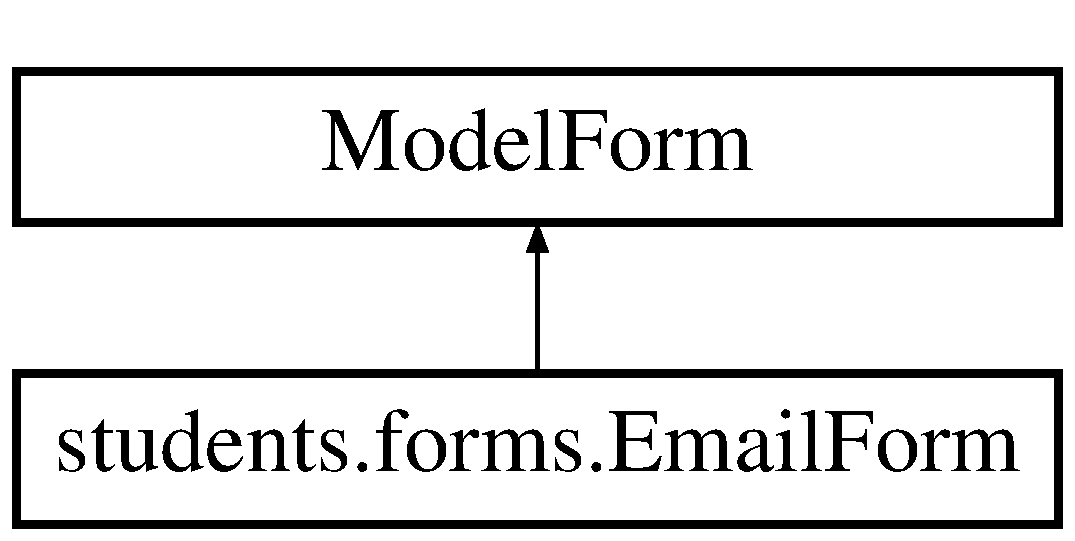
\includegraphics[height=2.000000cm]{classstudents_1_1forms_1_1_email_form}
\end{center}
\end{figure}
\subsection*{Classes}
\begin{DoxyCompactItemize}
\item 
class \hyperlink{classstudents_1_1forms_1_1_email_form_1_1_meta}{Meta}
\end{DoxyCompactItemize}
\subsection*{Public Member Functions}
\begin{DoxyCompactItemize}
\item 
def \hyperlink{classstudents_1_1forms_1_1_email_form_a4eb033bcad97e7be2130240400d707bf}{\-\_\-\-\_\-init\-\_\-\-\_\-}
\end{DoxyCompactItemize}
\subsection*{Public Attributes}
\begin{DoxyCompactItemize}
\item 
\hyperlink{classstudents_1_1forms_1_1_email_form_a23d2d15aeb526e44e16a34f2a92a7ee6}{helper}
\end{DoxyCompactItemize}
\subsection*{Static Public Attributes}
\begin{DoxyCompactItemize}
\item 
tuple \hyperlink{classstudents_1_1forms_1_1_email_form_a7bd89f273fdaea098b00a967c3594262}{subject} = forms.\-Char\-Field(max\-\_\-length=100)
\item 
tuple \hyperlink{classstudents_1_1forms_1_1_email_form_a8ef5a3b6972459707166e4b96b06d187}{body} = forms.\-Char\-Field(widget=forms.\-Textarea)
\item 
tuple \hyperlink{classstudents_1_1forms_1_1_email_form_a665a24f8008c7bfaa174dd25decca0b0}{attachment} = forms.\-File\-Field(required=False,)
\end{DoxyCompactItemize}


\subsection{Constructor \& Destructor Documentation}
\hypertarget{classstudents_1_1forms_1_1_email_form_a4eb033bcad97e7be2130240400d707bf}{\index{students\-::forms\-::\-Email\-Form@{students\-::forms\-::\-Email\-Form}!\-\_\-\-\_\-init\-\_\-\-\_\-@{\-\_\-\-\_\-init\-\_\-\-\_\-}}
\index{\-\_\-\-\_\-init\-\_\-\-\_\-@{\-\_\-\-\_\-init\-\_\-\-\_\-}!students::forms::EmailForm@{students\-::forms\-::\-Email\-Form}}
\subsubsection[{\-\_\-\-\_\-init\-\_\-\-\_\-}]{\setlength{\rightskip}{0pt plus 5cm}def students.\-forms.\-Email\-Form.\-\_\-\-\_\-init\-\_\-\-\_\- (
\begin{DoxyParamCaption}
\item[{}]{self, }
\item[{}]{args, }
\item[{}]{kwargs}
\end{DoxyParamCaption}
)}}\label{classstudents_1_1forms_1_1_email_form_a4eb033bcad97e7be2130240400d707bf}


\subsection{Member Data Documentation}
\hypertarget{classstudents_1_1forms_1_1_email_form_a665a24f8008c7bfaa174dd25decca0b0}{\index{students\-::forms\-::\-Email\-Form@{students\-::forms\-::\-Email\-Form}!attachment@{attachment}}
\index{attachment@{attachment}!students::forms::EmailForm@{students\-::forms\-::\-Email\-Form}}
\subsubsection[{attachment}]{\setlength{\rightskip}{0pt plus 5cm}tuple students.\-forms.\-Email\-Form.\-attachment = forms.\-File\-Field(required=False,)\hspace{0.3cm}{\ttfamily [static]}}}\label{classstudents_1_1forms_1_1_email_form_a665a24f8008c7bfaa174dd25decca0b0}
\hypertarget{classstudents_1_1forms_1_1_email_form_a8ef5a3b6972459707166e4b96b06d187}{\index{students\-::forms\-::\-Email\-Form@{students\-::forms\-::\-Email\-Form}!body@{body}}
\index{body@{body}!students::forms::EmailForm@{students\-::forms\-::\-Email\-Form}}
\subsubsection[{body}]{\setlength{\rightskip}{0pt plus 5cm}tuple students.\-forms.\-Email\-Form.\-body = forms.\-Char\-Field(widget=forms.\-Textarea)\hspace{0.3cm}{\ttfamily [static]}}}\label{classstudents_1_1forms_1_1_email_form_a8ef5a3b6972459707166e4b96b06d187}
\hypertarget{classstudents_1_1forms_1_1_email_form_a23d2d15aeb526e44e16a34f2a92a7ee6}{\index{students\-::forms\-::\-Email\-Form@{students\-::forms\-::\-Email\-Form}!helper@{helper}}
\index{helper@{helper}!students::forms::EmailForm@{students\-::forms\-::\-Email\-Form}}
\subsubsection[{helper}]{\setlength{\rightskip}{0pt plus 5cm}students.\-forms.\-Email\-Form.\-helper}}\label{classstudents_1_1forms_1_1_email_form_a23d2d15aeb526e44e16a34f2a92a7ee6}
\hypertarget{classstudents_1_1forms_1_1_email_form_a7bd89f273fdaea098b00a967c3594262}{\index{students\-::forms\-::\-Email\-Form@{students\-::forms\-::\-Email\-Form}!subject@{subject}}
\index{subject@{subject}!students::forms::EmailForm@{students\-::forms\-::\-Email\-Form}}
\subsubsection[{subject}]{\setlength{\rightskip}{0pt plus 5cm}tuple students.\-forms.\-Email\-Form.\-subject = forms.\-Char\-Field(max\-\_\-length=100)\hspace{0.3cm}{\ttfamily [static]}}}\label{classstudents_1_1forms_1_1_email_form_a7bd89f273fdaea098b00a967c3594262}


The documentation for this class was generated from the following file\-:\begin{DoxyCompactItemize}
\item 
leapkit/students/\hyperlink{forms_8py}{forms.\-py}\end{DoxyCompactItemize}

\hypertarget{classstudents_1_1models_1_1_language}{\section{students.\-models.\-Language Class Reference}
\label{classstudents_1_1models_1_1_language}\index{students.\-models.\-Language@{students.\-models.\-Language}}
}
Inheritance diagram for students.\-models.\-Language\-:\begin{figure}[H]
\begin{center}
\leavevmode
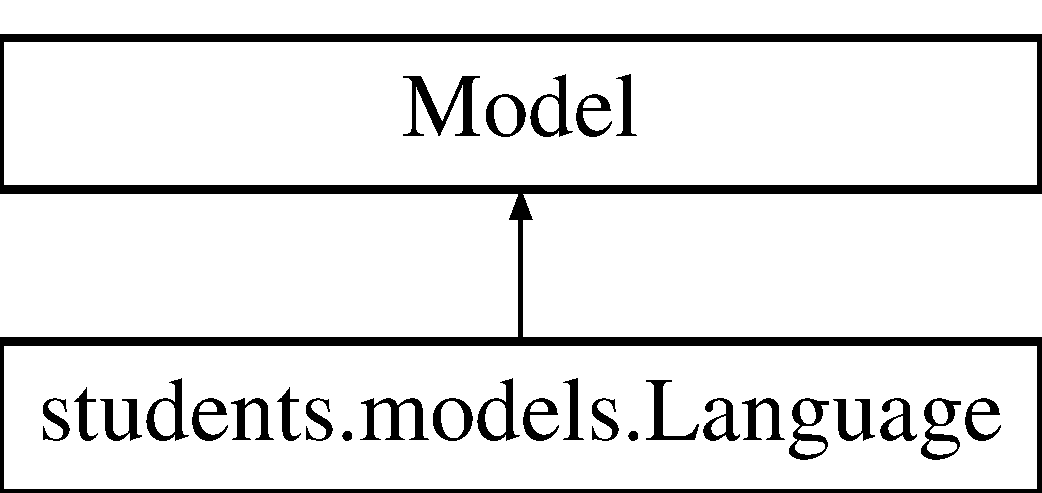
\includegraphics[height=2.000000cm]{classstudents_1_1models_1_1_language}
\end{center}
\end{figure}
\subsection*{Public Member Functions}
\begin{DoxyCompactItemize}
\item 
def \hyperlink{classstudents_1_1models_1_1_language_a656e053c3a3adce525fb3a3b000d08b1}{\-\_\-\-\_\-unicode\-\_\-\-\_\-}
\item 
def \hyperlink{classstudents_1_1models_1_1_language_a5b15a386a956f22ce3507f94f57cbf60}{get\-\_\-language}
\end{DoxyCompactItemize}
\subsection*{Static Public Attributes}
\begin{DoxyCompactItemize}
\item 
tuple \hyperlink{classstudents_1_1models_1_1_language_ac37164d4a1b3ac7c31546adfe1dd18d5}{name} = models.\-Char\-Field(max\-\_\-length = 30)
\item 
tuple \hyperlink{classstudents_1_1models_1_1_language_affd66c68817bac13ece99da9eca10101}{level} = models.\-Char\-Field(max\-\_\-length = 30)
\item 
tuple \hyperlink{classstudents_1_1models_1_1_language_ab9c9571762a4e0df5dda38d8ad451c3d}{profile} = models.\-Foreign\-Key(\hyperlink{classstudents_1_1models_1_1_linked_in_profile}{Linked\-In\-Profile})
\end{DoxyCompactItemize}


\subsection{Detailed Description}
\begin{DoxyVerb}Model that represents a language on LinkedIn.
\end{DoxyVerb}
 

\subsection{Member Function Documentation}
\hypertarget{classstudents_1_1models_1_1_language_a656e053c3a3adce525fb3a3b000d08b1}{\index{students\-::models\-::\-Language@{students\-::models\-::\-Language}!\-\_\-\-\_\-unicode\-\_\-\-\_\-@{\-\_\-\-\_\-unicode\-\_\-\-\_\-}}
\index{\-\_\-\-\_\-unicode\-\_\-\-\_\-@{\-\_\-\-\_\-unicode\-\_\-\-\_\-}!students::models::Language@{students\-::models\-::\-Language}}
\subsubsection[{\-\_\-\-\_\-unicode\-\_\-\-\_\-}]{\setlength{\rightskip}{0pt plus 5cm}def students.\-models.\-Language.\-\_\-\-\_\-unicode\-\_\-\-\_\- (
\begin{DoxyParamCaption}
\item[{}]{self}
\end{DoxyParamCaption}
)}}\label{classstudents_1_1models_1_1_language_a656e053c3a3adce525fb3a3b000d08b1}
\hypertarget{classstudents_1_1models_1_1_language_a5b15a386a956f22ce3507f94f57cbf60}{\index{students\-::models\-::\-Language@{students\-::models\-::\-Language}!get\-\_\-language@{get\-\_\-language}}
\index{get\-\_\-language@{get\-\_\-language}!students::models::Language@{students\-::models\-::\-Language}}
\subsubsection[{get\-\_\-language}]{\setlength{\rightskip}{0pt plus 5cm}def students.\-models.\-Language.\-get\-\_\-language (
\begin{DoxyParamCaption}
\item[{}]{self}
\end{DoxyParamCaption}
)}}\label{classstudents_1_1models_1_1_language_a5b15a386a956f22ce3507f94f57cbf60}


\subsection{Member Data Documentation}
\hypertarget{classstudents_1_1models_1_1_language_affd66c68817bac13ece99da9eca10101}{\index{students\-::models\-::\-Language@{students\-::models\-::\-Language}!level@{level}}
\index{level@{level}!students::models::Language@{students\-::models\-::\-Language}}
\subsubsection[{level}]{\setlength{\rightskip}{0pt plus 5cm}tuple students.\-models.\-Language.\-level = models.\-Char\-Field(max\-\_\-length = 30)\hspace{0.3cm}{\ttfamily [static]}}}\label{classstudents_1_1models_1_1_language_affd66c68817bac13ece99da9eca10101}
\hypertarget{classstudents_1_1models_1_1_language_ac37164d4a1b3ac7c31546adfe1dd18d5}{\index{students\-::models\-::\-Language@{students\-::models\-::\-Language}!name@{name}}
\index{name@{name}!students::models::Language@{students\-::models\-::\-Language}}
\subsubsection[{name}]{\setlength{\rightskip}{0pt plus 5cm}tuple students.\-models.\-Language.\-name = models.\-Char\-Field(max\-\_\-length = 30)\hspace{0.3cm}{\ttfamily [static]}}}\label{classstudents_1_1models_1_1_language_ac37164d4a1b3ac7c31546adfe1dd18d5}
\hypertarget{classstudents_1_1models_1_1_language_ab9c9571762a4e0df5dda38d8ad451c3d}{\index{students\-::models\-::\-Language@{students\-::models\-::\-Language}!profile@{profile}}
\index{profile@{profile}!students::models::Language@{students\-::models\-::\-Language}}
\subsubsection[{profile}]{\setlength{\rightskip}{0pt plus 5cm}tuple students.\-models.\-Language.\-profile = models.\-Foreign\-Key({\bf Linked\-In\-Profile})\hspace{0.3cm}{\ttfamily [static]}}}\label{classstudents_1_1models_1_1_language_ab9c9571762a4e0df5dda38d8ad451c3d}


The documentation for this class was generated from the following file\-:\begin{DoxyCompactItemize}
\item 
leapkit/students/\hyperlink{models_8py}{models.\-py}\end{DoxyCompactItemize}

\hypertarget{classstudents_1_1linkedin__converter_1_1_language}{\section{students.\-linkedin\-\_\-converter.\-Language Class Reference}
\label{classstudents_1_1linkedin__converter_1_1_language}\index{students.\-linkedin\-\_\-converter.\-Language@{students.\-linkedin\-\_\-converter.\-Language}}
}
Inheritance diagram for students.\-linkedin\-\_\-converter.\-Language\-:\begin{figure}[H]
\begin{center}
\leavevmode
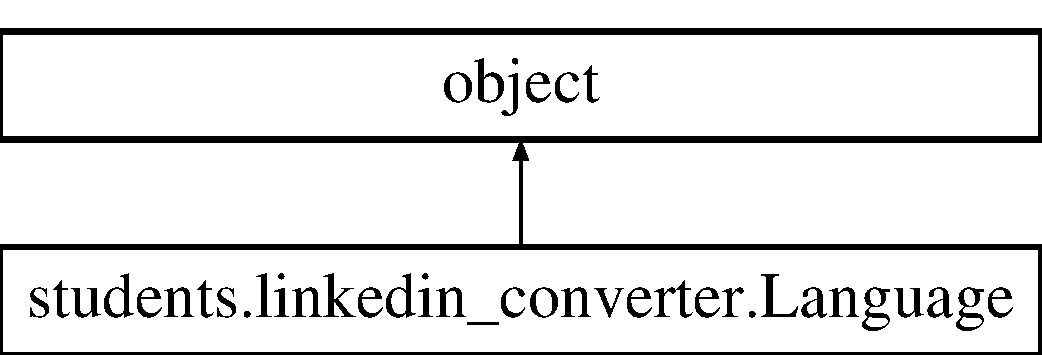
\includegraphics[height=2.000000cm]{classstudents_1_1linkedin__converter_1_1_language}
\end{center}
\end{figure}
\subsection*{Static Public Attributes}
\begin{DoxyCompactItemize}
\item 
string \hyperlink{classstudents_1_1linkedin__converter_1_1_language_a6da003395448aa81cf8c21c7c8d82631}{lid} = \char`\"{}\char`\"{}
\item 
string \hyperlink{classstudents_1_1linkedin__converter_1_1_language_a49e40399b6750244a4ceb0af02735441}{name} = \char`\"{}\char`\"{}
\item 
string \hyperlink{classstudents_1_1linkedin__converter_1_1_language_a8f85e43a3425592d3b1b65aae235d098}{level} = \char`\"{}\char`\"{}
\end{DoxyCompactItemize}


\subsection{Detailed Description}
\begin{DoxyVerb}A Language is used to hold the languages and profifiency the person knows.\end{DoxyVerb}
\begin{DoxyVerb}Constructor that initiates all the basic language values\end{DoxyVerb}
 

\subsection{Member Data Documentation}
\hypertarget{classstudents_1_1linkedin__converter_1_1_language_a8f85e43a3425592d3b1b65aae235d098}{\index{students\-::linkedin\-\_\-converter\-::\-Language@{students\-::linkedin\-\_\-converter\-::\-Language}!level@{level}}
\index{level@{level}!students::linkedin_converter::Language@{students\-::linkedin\-\_\-converter\-::\-Language}}
\subsubsection[{level}]{\setlength{\rightskip}{0pt plus 5cm}string students.\-linkedin\-\_\-converter.\-Language.\-level = \char`\"{}\char`\"{}\hspace{0.3cm}{\ttfamily [static]}}}\label{classstudents_1_1linkedin__converter_1_1_language_a8f85e43a3425592d3b1b65aae235d098}
\hypertarget{classstudents_1_1linkedin__converter_1_1_language_a6da003395448aa81cf8c21c7c8d82631}{\index{students\-::linkedin\-\_\-converter\-::\-Language@{students\-::linkedin\-\_\-converter\-::\-Language}!lid@{lid}}
\index{lid@{lid}!students::linkedin_converter::Language@{students\-::linkedin\-\_\-converter\-::\-Language}}
\subsubsection[{lid}]{\setlength{\rightskip}{0pt plus 5cm}string students.\-linkedin\-\_\-converter.\-Language.\-lid = \char`\"{}\char`\"{}\hspace{0.3cm}{\ttfamily [static]}}}\label{classstudents_1_1linkedin__converter_1_1_language_a6da003395448aa81cf8c21c7c8d82631}
\hypertarget{classstudents_1_1linkedin__converter_1_1_language_a49e40399b6750244a4ceb0af02735441}{\index{students\-::linkedin\-\_\-converter\-::\-Language@{students\-::linkedin\-\_\-converter\-::\-Language}!name@{name}}
\index{name@{name}!students::linkedin_converter::Language@{students\-::linkedin\-\_\-converter\-::\-Language}}
\subsubsection[{name}]{\setlength{\rightskip}{0pt plus 5cm}string students.\-linkedin\-\_\-converter.\-Language.\-name = \char`\"{}\char`\"{}\hspace{0.3cm}{\ttfamily [static]}}}\label{classstudents_1_1linkedin__converter_1_1_language_a49e40399b6750244a4ceb0af02735441}


The documentation for this class was generated from the following file\-:\begin{DoxyCompactItemize}
\item 
leapkit/students/\hyperlink{linkedin__converter_8py}{linkedin\-\_\-converter.\-py}\end{DoxyCompactItemize}

\hypertarget{classstudents_1_1admin_1_1_language_admin}{\section{students.\-admin.\-Language\-Admin Class Reference}
\label{classstudents_1_1admin_1_1_language_admin}\index{students.\-admin.\-Language\-Admin@{students.\-admin.\-Language\-Admin}}
}
Inheritance diagram for students.\-admin.\-Language\-Admin\-:\begin{figure}[H]
\begin{center}
\leavevmode
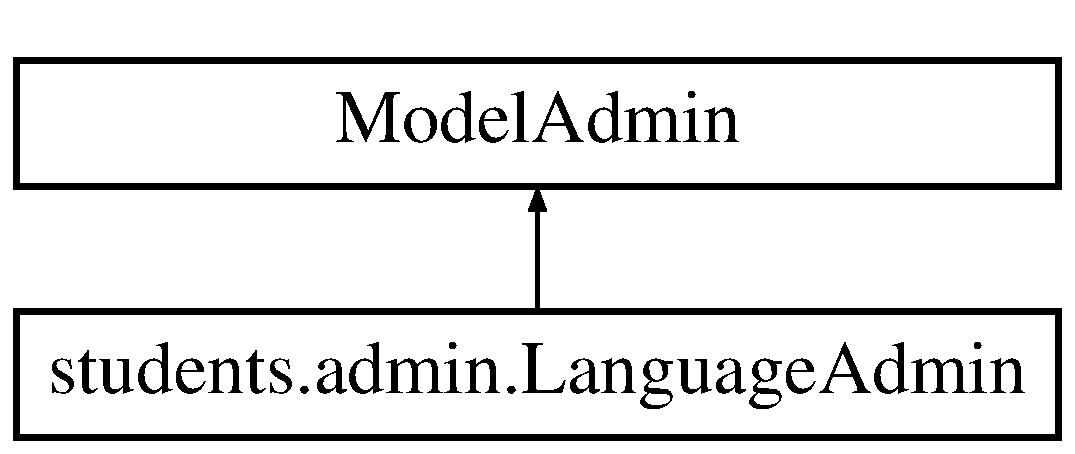
\includegraphics[height=2.000000cm]{classstudents_1_1admin_1_1_language_admin}
\end{center}
\end{figure}
\subsection*{Static Public Attributes}
\begin{DoxyCompactItemize}
\item 
list \hyperlink{classstudents_1_1admin_1_1_language_admin_adb64e35cb2808fcb92ba85970394ed60}{fieldsets} = \mbox{[}(None, \{'fields' \-: \mbox{[}'name', 'level','profile'\mbox{]}\}),\mbox{]}
\item 
tuple \hyperlink{classstudents_1_1admin_1_1_language_admin_a36a061d2b5f97c82377a82b5a611fe38}{list\-\_\-display} = ('name', 'level', 'profile')
\item 
list \hyperlink{classstudents_1_1admin_1_1_language_admin_a810be0e4fc8b533d9e02cc3bbe7bc1dc}{search\-\_\-fields} = \mbox{[}'name','level','profile'\mbox{]}
\end{DoxyCompactItemize}


\subsection{Member Data Documentation}
\hypertarget{classstudents_1_1admin_1_1_language_admin_adb64e35cb2808fcb92ba85970394ed60}{\index{students\-::admin\-::\-Language\-Admin@{students\-::admin\-::\-Language\-Admin}!fieldsets@{fieldsets}}
\index{fieldsets@{fieldsets}!students::admin::LanguageAdmin@{students\-::admin\-::\-Language\-Admin}}
\subsubsection[{fieldsets}]{\setlength{\rightskip}{0pt plus 5cm}list students.\-admin.\-Language\-Admin.\-fieldsets = \mbox{[}(None, \{'fields' \-: \mbox{[}'name', 'level','profile'\mbox{]}\}),\mbox{]}\hspace{0.3cm}{\ttfamily [static]}}}\label{classstudents_1_1admin_1_1_language_admin_adb64e35cb2808fcb92ba85970394ed60}
\hypertarget{classstudents_1_1admin_1_1_language_admin_a36a061d2b5f97c82377a82b5a611fe38}{\index{students\-::admin\-::\-Language\-Admin@{students\-::admin\-::\-Language\-Admin}!list\-\_\-display@{list\-\_\-display}}
\index{list\-\_\-display@{list\-\_\-display}!students::admin::LanguageAdmin@{students\-::admin\-::\-Language\-Admin}}
\subsubsection[{list\-\_\-display}]{\setlength{\rightskip}{0pt plus 5cm}tuple students.\-admin.\-Language\-Admin.\-list\-\_\-display = ('name', 'level', 'profile')\hspace{0.3cm}{\ttfamily [static]}}}\label{classstudents_1_1admin_1_1_language_admin_a36a061d2b5f97c82377a82b5a611fe38}
\hypertarget{classstudents_1_1admin_1_1_language_admin_a810be0e4fc8b533d9e02cc3bbe7bc1dc}{\index{students\-::admin\-::\-Language\-Admin@{students\-::admin\-::\-Language\-Admin}!search\-\_\-fields@{search\-\_\-fields}}
\index{search\-\_\-fields@{search\-\_\-fields}!students::admin::LanguageAdmin@{students\-::admin\-::\-Language\-Admin}}
\subsubsection[{search\-\_\-fields}]{\setlength{\rightskip}{0pt plus 5cm}list students.\-admin.\-Language\-Admin.\-search\-\_\-fields = \mbox{[}'name','level','profile'\mbox{]}\hspace{0.3cm}{\ttfamily [static]}}}\label{classstudents_1_1admin_1_1_language_admin_a810be0e4fc8b533d9e02cc3bbe7bc1dc}


The documentation for this class was generated from the following file\-:\begin{DoxyCompactItemize}
\item 
leapkit/students/\hyperlink{admin_8py}{admin.\-py}\end{DoxyCompactItemize}

\hypertarget{classstudents_1_1models_1_1_linked_in_profile}{\section{students.\-models.\-Linked\-In\-Profile Class Reference}
\label{classstudents_1_1models_1_1_linked_in_profile}\index{students.\-models.\-Linked\-In\-Profile@{students.\-models.\-Linked\-In\-Profile}}
}
Inheritance diagram for students.\-models.\-Linked\-In\-Profile\-:\begin{figure}[H]
\begin{center}
\leavevmode
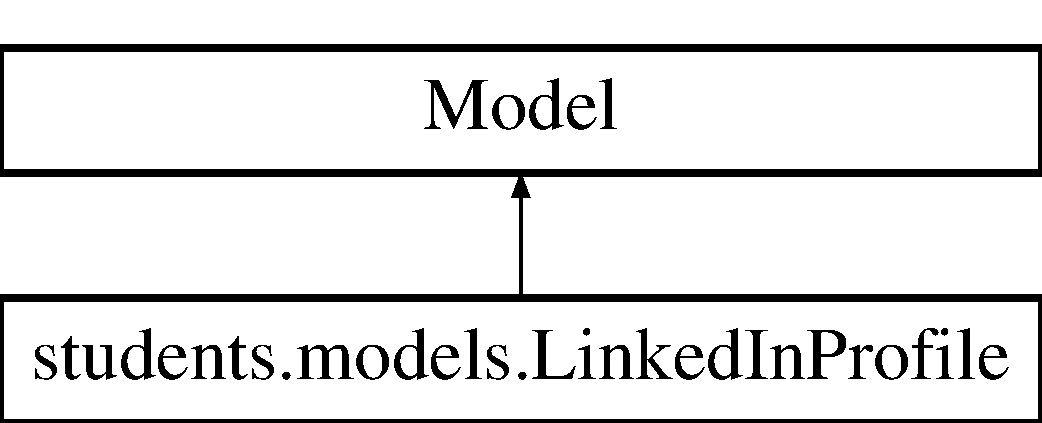
\includegraphics[height=2.000000cm]{classstudents_1_1models_1_1_linked_in_profile}
\end{center}
\end{figure}
\subsection*{Public Member Functions}
\begin{DoxyCompactItemize}
\item 
def \hyperlink{classstudents_1_1models_1_1_linked_in_profile_a625f309407380b0239ed0ba4a8fcd8f8}{\-\_\-\-\_\-unicode\-\_\-\-\_\-}
\item 
def \hyperlink{classstudents_1_1models_1_1_linked_in_profile_af7294caa5c9dd7dc43bed9b4ff962e20}{get\-\_\-full\-\_\-name}
\end{DoxyCompactItemize}
\subsection*{Static Public Attributes}
\begin{DoxyCompactItemize}
\item 
tuple \hyperlink{classstudents_1_1models_1_1_linked_in_profile_ac0b6bb95d0354a37b69a74c261ee67cb}{leapkituser} = models.\-One\-To\-One\-Field(User)
\item 
tuple \hyperlink{classstudents_1_1models_1_1_linked_in_profile_a5a40a9ab44852b841f9ec30b5351b46f}{modified} = models.\-Date\-Time\-Field('modified', auto\-\_\-now=True)
\item 
tuple \hyperlink{classstudents_1_1models_1_1_linked_in_profile_a9ec9270281a1ed7cc744f3a027dbdc01}{linkedin\-\_\-id} = models.\-Text\-Field()
\item 
tuple \hyperlink{classstudents_1_1models_1_1_linked_in_profile_a8fedcda58ba560b252b16404f83feb5e}{first\-Name} = models.\-Text\-Field()
\item 
tuple \hyperlink{classstudents_1_1models_1_1_linked_in_profile_ad8ce210760752fd163191757482008bc}{last\-Name} = models.\-Text\-Field()
\item 
tuple \hyperlink{classstudents_1_1models_1_1_linked_in_profile_aa6723daf0868233192944d27c627a0be}{picture\-Url} = models.\-Text\-Field(null=True, blank=True)
\item 
tuple \hyperlink{classstudents_1_1models_1_1_linked_in_profile_a4ca4e96f931603cea56405a4c6ca2c31}{public\-Profile\-Url} = models.\-Text\-Field(null=True, blank=True)
\end{DoxyCompactItemize}


\subsection{Detailed Description}
\begin{DoxyVerb}This model is used to represent a students LinkedIn information.
\end{DoxyVerb}
 

\subsection{Member Function Documentation}
\hypertarget{classstudents_1_1models_1_1_linked_in_profile_a625f309407380b0239ed0ba4a8fcd8f8}{\index{students\-::models\-::\-Linked\-In\-Profile@{students\-::models\-::\-Linked\-In\-Profile}!\-\_\-\-\_\-unicode\-\_\-\-\_\-@{\-\_\-\-\_\-unicode\-\_\-\-\_\-}}
\index{\-\_\-\-\_\-unicode\-\_\-\-\_\-@{\-\_\-\-\_\-unicode\-\_\-\-\_\-}!students::models::LinkedInProfile@{students\-::models\-::\-Linked\-In\-Profile}}
\subsubsection[{\-\_\-\-\_\-unicode\-\_\-\-\_\-}]{\setlength{\rightskip}{0pt plus 5cm}def students.\-models.\-Linked\-In\-Profile.\-\_\-\-\_\-unicode\-\_\-\-\_\- (
\begin{DoxyParamCaption}
\item[{}]{self}
\end{DoxyParamCaption}
)}}\label{classstudents_1_1models_1_1_linked_in_profile_a625f309407380b0239ed0ba4a8fcd8f8}
\hypertarget{classstudents_1_1models_1_1_linked_in_profile_af7294caa5c9dd7dc43bed9b4ff962e20}{\index{students\-::models\-::\-Linked\-In\-Profile@{students\-::models\-::\-Linked\-In\-Profile}!get\-\_\-full\-\_\-name@{get\-\_\-full\-\_\-name}}
\index{get\-\_\-full\-\_\-name@{get\-\_\-full\-\_\-name}!students::models::LinkedInProfile@{students\-::models\-::\-Linked\-In\-Profile}}
\subsubsection[{get\-\_\-full\-\_\-name}]{\setlength{\rightskip}{0pt plus 5cm}def students.\-models.\-Linked\-In\-Profile.\-get\-\_\-full\-\_\-name (
\begin{DoxyParamCaption}
\item[{}]{self}
\end{DoxyParamCaption}
)}}\label{classstudents_1_1models_1_1_linked_in_profile_af7294caa5c9dd7dc43bed9b4ff962e20}
\begin{DoxyVerb}:return: First name + last name, with a space in between
\end{DoxyVerb}
 

\subsection{Member Data Documentation}
\hypertarget{classstudents_1_1models_1_1_linked_in_profile_a8fedcda58ba560b252b16404f83feb5e}{\index{students\-::models\-::\-Linked\-In\-Profile@{students\-::models\-::\-Linked\-In\-Profile}!first\-Name@{first\-Name}}
\index{first\-Name@{first\-Name}!students::models::LinkedInProfile@{students\-::models\-::\-Linked\-In\-Profile}}
\subsubsection[{first\-Name}]{\setlength{\rightskip}{0pt plus 5cm}tuple students.\-models.\-Linked\-In\-Profile.\-first\-Name = models.\-Text\-Field()\hspace{0.3cm}{\ttfamily [static]}}}\label{classstudents_1_1models_1_1_linked_in_profile_a8fedcda58ba560b252b16404f83feb5e}
\hypertarget{classstudents_1_1models_1_1_linked_in_profile_ad8ce210760752fd163191757482008bc}{\index{students\-::models\-::\-Linked\-In\-Profile@{students\-::models\-::\-Linked\-In\-Profile}!last\-Name@{last\-Name}}
\index{last\-Name@{last\-Name}!students::models::LinkedInProfile@{students\-::models\-::\-Linked\-In\-Profile}}
\subsubsection[{last\-Name}]{\setlength{\rightskip}{0pt plus 5cm}tuple students.\-models.\-Linked\-In\-Profile.\-last\-Name = models.\-Text\-Field()\hspace{0.3cm}{\ttfamily [static]}}}\label{classstudents_1_1models_1_1_linked_in_profile_ad8ce210760752fd163191757482008bc}
\hypertarget{classstudents_1_1models_1_1_linked_in_profile_ac0b6bb95d0354a37b69a74c261ee67cb}{\index{students\-::models\-::\-Linked\-In\-Profile@{students\-::models\-::\-Linked\-In\-Profile}!leapkituser@{leapkituser}}
\index{leapkituser@{leapkituser}!students::models::LinkedInProfile@{students\-::models\-::\-Linked\-In\-Profile}}
\subsubsection[{leapkituser}]{\setlength{\rightskip}{0pt plus 5cm}tuple students.\-models.\-Linked\-In\-Profile.\-leapkituser = models.\-One\-To\-One\-Field(User)\hspace{0.3cm}{\ttfamily [static]}}}\label{classstudents_1_1models_1_1_linked_in_profile_ac0b6bb95d0354a37b69a74c261ee67cb}
\hypertarget{classstudents_1_1models_1_1_linked_in_profile_a9ec9270281a1ed7cc744f3a027dbdc01}{\index{students\-::models\-::\-Linked\-In\-Profile@{students\-::models\-::\-Linked\-In\-Profile}!linkedin\-\_\-id@{linkedin\-\_\-id}}
\index{linkedin\-\_\-id@{linkedin\-\_\-id}!students::models::LinkedInProfile@{students\-::models\-::\-Linked\-In\-Profile}}
\subsubsection[{linkedin\-\_\-id}]{\setlength{\rightskip}{0pt plus 5cm}tuple students.\-models.\-Linked\-In\-Profile.\-linkedin\-\_\-id = models.\-Text\-Field()\hspace{0.3cm}{\ttfamily [static]}}}\label{classstudents_1_1models_1_1_linked_in_profile_a9ec9270281a1ed7cc744f3a027dbdc01}
\hypertarget{classstudents_1_1models_1_1_linked_in_profile_a5a40a9ab44852b841f9ec30b5351b46f}{\index{students\-::models\-::\-Linked\-In\-Profile@{students\-::models\-::\-Linked\-In\-Profile}!modified@{modified}}
\index{modified@{modified}!students::models::LinkedInProfile@{students\-::models\-::\-Linked\-In\-Profile}}
\subsubsection[{modified}]{\setlength{\rightskip}{0pt plus 5cm}tuple students.\-models.\-Linked\-In\-Profile.\-modified = models.\-Date\-Time\-Field('modified', auto\-\_\-now=True)\hspace{0.3cm}{\ttfamily [static]}}}\label{classstudents_1_1models_1_1_linked_in_profile_a5a40a9ab44852b841f9ec30b5351b46f}
\hypertarget{classstudents_1_1models_1_1_linked_in_profile_aa6723daf0868233192944d27c627a0be}{\index{students\-::models\-::\-Linked\-In\-Profile@{students\-::models\-::\-Linked\-In\-Profile}!picture\-Url@{picture\-Url}}
\index{picture\-Url@{picture\-Url}!students::models::LinkedInProfile@{students\-::models\-::\-Linked\-In\-Profile}}
\subsubsection[{picture\-Url}]{\setlength{\rightskip}{0pt plus 5cm}tuple students.\-models.\-Linked\-In\-Profile.\-picture\-Url = models.\-Text\-Field(null=True, blank=True)\hspace{0.3cm}{\ttfamily [static]}}}\label{classstudents_1_1models_1_1_linked_in_profile_aa6723daf0868233192944d27c627a0be}
\hypertarget{classstudents_1_1models_1_1_linked_in_profile_a4ca4e96f931603cea56405a4c6ca2c31}{\index{students\-::models\-::\-Linked\-In\-Profile@{students\-::models\-::\-Linked\-In\-Profile}!public\-Profile\-Url@{public\-Profile\-Url}}
\index{public\-Profile\-Url@{public\-Profile\-Url}!students::models::LinkedInProfile@{students\-::models\-::\-Linked\-In\-Profile}}
\subsubsection[{public\-Profile\-Url}]{\setlength{\rightskip}{0pt plus 5cm}tuple students.\-models.\-Linked\-In\-Profile.\-public\-Profile\-Url = models.\-Text\-Field(null=True, blank=True)\hspace{0.3cm}{\ttfamily [static]}}}\label{classstudents_1_1models_1_1_linked_in_profile_a4ca4e96f931603cea56405a4c6ca2c31}


The documentation for this class was generated from the following file\-:\begin{DoxyCompactItemize}
\item 
leapkit/students/\hyperlink{models_8py}{models.\-py}\end{DoxyCompactItemize}

\hypertarget{classstudents_1_1admin_1_1_linked_in_profile_admin}{\section{students.\-admin.\-Linked\-In\-Profile\-Admin Class Reference}
\label{classstudents_1_1admin_1_1_linked_in_profile_admin}\index{students.\-admin.\-Linked\-In\-Profile\-Admin@{students.\-admin.\-Linked\-In\-Profile\-Admin}}
}
Inheritance diagram for students.\-admin.\-Linked\-In\-Profile\-Admin\-:\begin{figure}[H]
\begin{center}
\leavevmode
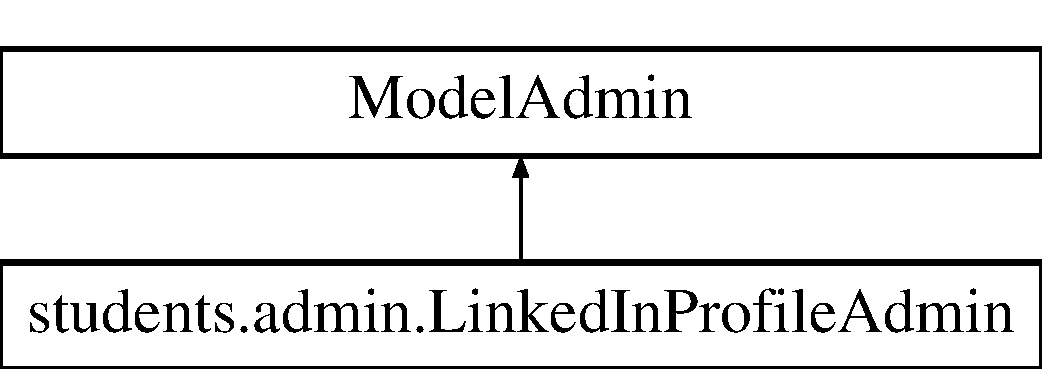
\includegraphics[height=2.000000cm]{classstudents_1_1admin_1_1_linked_in_profile_admin}
\end{center}
\end{figure}
\subsection*{Static Public Attributes}
\begin{DoxyCompactItemize}
\item 
list \hyperlink{classstudents_1_1admin_1_1_linked_in_profile_admin_a49860d8113b436c82419cdb40f94cf7e}{fieldsets}
\item 
tuple \hyperlink{classstudents_1_1admin_1_1_linked_in_profile_admin_abd0c2a04fc225eba9b673e20ff8e3f23}{readonly\-\_\-fields} = ('modified',)
\item 
tuple \hyperlink{classstudents_1_1admin_1_1_linked_in_profile_admin_ae5480d47cffc8596e57f5a3fa03dc0bb}{list\-\_\-display} = ('leapkituser', 'first\-Name', 'last\-Name', 'modified')
\item 
list \hyperlink{classstudents_1_1admin_1_1_linked_in_profile_admin_a6d9b8f11fae479f690c2db995e7a0bb5}{search\-\_\-fields} = \mbox{[}'leapkituser', 'first\-Name'\mbox{]}
\end{DoxyCompactItemize}


\subsection{Member Data Documentation}
\hypertarget{classstudents_1_1admin_1_1_linked_in_profile_admin_a49860d8113b436c82419cdb40f94cf7e}{\index{students\-::admin\-::\-Linked\-In\-Profile\-Admin@{students\-::admin\-::\-Linked\-In\-Profile\-Admin}!fieldsets@{fieldsets}}
\index{fieldsets@{fieldsets}!students::admin::LinkedInProfileAdmin@{students\-::admin\-::\-Linked\-In\-Profile\-Admin}}
\subsubsection[{fieldsets}]{\setlength{\rightskip}{0pt plus 5cm}list students.\-admin.\-Linked\-In\-Profile\-Admin.\-fieldsets\hspace{0.3cm}{\ttfamily [static]}}}\label{classstudents_1_1admin_1_1_linked_in_profile_admin_a49860d8113b436c82419cdb40f94cf7e}
{\bfseries Initial value\-:}
\begin{DoxyCode}
1 = [
2         (\textcolor{keywordtype}{None}, \{\textcolor{stringliteral}{'fields'}: [\textcolor{stringliteral}{'leapkituser'},
3                            \textcolor{stringliteral}{'linkedin\_id'},
4                            \textcolor{stringliteral}{'firstName'},
5                            \textcolor{stringliteral}{'lastName'},
6 \textcolor{comment}{#                          'positions',}
7 \textcolor{comment}{#                          'pictureUrl',}
8 \textcolor{comment}{#                          'publicProfileUrl'}
9                            ]\}),
10     ]
\end{DoxyCode}
\hypertarget{classstudents_1_1admin_1_1_linked_in_profile_admin_ae5480d47cffc8596e57f5a3fa03dc0bb}{\index{students\-::admin\-::\-Linked\-In\-Profile\-Admin@{students\-::admin\-::\-Linked\-In\-Profile\-Admin}!list\-\_\-display@{list\-\_\-display}}
\index{list\-\_\-display@{list\-\_\-display}!students::admin::LinkedInProfileAdmin@{students\-::admin\-::\-Linked\-In\-Profile\-Admin}}
\subsubsection[{list\-\_\-display}]{\setlength{\rightskip}{0pt plus 5cm}tuple students.\-admin.\-Linked\-In\-Profile\-Admin.\-list\-\_\-display = ('leapkituser', 'first\-Name', 'last\-Name', 'modified')\hspace{0.3cm}{\ttfamily [static]}}}\label{classstudents_1_1admin_1_1_linked_in_profile_admin_ae5480d47cffc8596e57f5a3fa03dc0bb}
\hypertarget{classstudents_1_1admin_1_1_linked_in_profile_admin_abd0c2a04fc225eba9b673e20ff8e3f23}{\index{students\-::admin\-::\-Linked\-In\-Profile\-Admin@{students\-::admin\-::\-Linked\-In\-Profile\-Admin}!readonly\-\_\-fields@{readonly\-\_\-fields}}
\index{readonly\-\_\-fields@{readonly\-\_\-fields}!students::admin::LinkedInProfileAdmin@{students\-::admin\-::\-Linked\-In\-Profile\-Admin}}
\subsubsection[{readonly\-\_\-fields}]{\setlength{\rightskip}{0pt plus 5cm}tuple students.\-admin.\-Linked\-In\-Profile\-Admin.\-readonly\-\_\-fields = ('modified',)\hspace{0.3cm}{\ttfamily [static]}}}\label{classstudents_1_1admin_1_1_linked_in_profile_admin_abd0c2a04fc225eba9b673e20ff8e3f23}
\hypertarget{classstudents_1_1admin_1_1_linked_in_profile_admin_a6d9b8f11fae479f690c2db995e7a0bb5}{\index{students\-::admin\-::\-Linked\-In\-Profile\-Admin@{students\-::admin\-::\-Linked\-In\-Profile\-Admin}!search\-\_\-fields@{search\-\_\-fields}}
\index{search\-\_\-fields@{search\-\_\-fields}!students::admin::LinkedInProfileAdmin@{students\-::admin\-::\-Linked\-In\-Profile\-Admin}}
\subsubsection[{search\-\_\-fields}]{\setlength{\rightskip}{0pt plus 5cm}list students.\-admin.\-Linked\-In\-Profile\-Admin.\-search\-\_\-fields = \mbox{[}'leapkituser', 'first\-Name'\mbox{]}\hspace{0.3cm}{\ttfamily [static]}}}\label{classstudents_1_1admin_1_1_linked_in_profile_admin_a6d9b8f11fae479f690c2db995e7a0bb5}


The documentation for this class was generated from the following file\-:\begin{DoxyCompactItemize}
\item 
leapkit/students/\hyperlink{admin_8py}{admin.\-py}\end{DoxyCompactItemize}

\hypertarget{classstudents_1_1views_1_1_list_all_projects_view}{\section{students.\-views.\-List\-All\-Projects\-View Class Reference}
\label{classstudents_1_1views_1_1_list_all_projects_view}\index{students.\-views.\-List\-All\-Projects\-View@{students.\-views.\-List\-All\-Projects\-View}}
}
Inheritance diagram for students.\-views.\-List\-All\-Projects\-View\-:\begin{figure}[H]
\begin{center}
\leavevmode
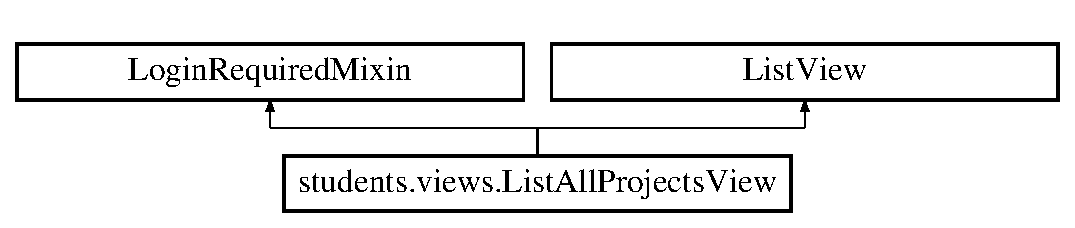
\includegraphics[height=2.000000cm]{classstudents_1_1views_1_1_list_all_projects_view}
\end{center}
\end{figure}
\subsection*{Public Member Functions}
\begin{DoxyCompactItemize}
\item 
def \hyperlink{classstudents_1_1views_1_1_list_all_projects_view_a0d33266bd02b1a7db4bcadb7013a02ad}{dispatch}
\item 
def \hyperlink{classstudents_1_1views_1_1_list_all_projects_view_a97ba8473b483cd8c26dfdc1a68c71488}{get\-\_\-queryset}
\item 
def \hyperlink{classstudents_1_1views_1_1_list_all_projects_view_aa3c93985310036111318a294b02c4c6e}{get\-\_\-context\-\_\-data}
\end{DoxyCompactItemize}
\subsection*{Static Public Attributes}
\begin{DoxyCompactItemize}
\item 
string \hyperlink{classstudents_1_1views_1_1_list_all_projects_view_ab06ec282a4c4a4961f2bf7dc0fd60488}{template\-\_\-name} = \char`\"{}list\-\_\-all\-\_\-projects.\-html\char`\"{}
\item 
string \hyperlink{classstudents_1_1views_1_1_list_all_projects_view_a54749455487671085d05067dd5393485}{login\-\_\-url} = \char`\"{}/students/login/\char`\"{}
\item 
\hyperlink{classstudents_1_1views_1_1_list_all_projects_view_aacf6369cc6f66b902ddc325d9f73d0ca}{model} = Project
\item 
int \hyperlink{classstudents_1_1views_1_1_list_all_projects_view_a4b0bc6c6be4be3fd1bdaf6b886dffd61}{paginate\-\_\-by} = 20
\item 
\hyperlink{classstudents_1_1views_1_1_list_all_projects_view_a9976aeeb2c980ed4ecc8715d52a1fe17}{allow\-\_\-empty} = True
\end{DoxyCompactItemize}


\subsection{Member Function Documentation}
\hypertarget{classstudents_1_1views_1_1_list_all_projects_view_a0d33266bd02b1a7db4bcadb7013a02ad}{\index{students\-::views\-::\-List\-All\-Projects\-View@{students\-::views\-::\-List\-All\-Projects\-View}!dispatch@{dispatch}}
\index{dispatch@{dispatch}!students::views::ListAllProjectsView@{students\-::views\-::\-List\-All\-Projects\-View}}
\subsubsection[{dispatch}]{\setlength{\rightskip}{0pt plus 5cm}def students.\-views.\-List\-All\-Projects\-View.\-dispatch (
\begin{DoxyParamCaption}
\item[{}]{self, }
\item[{}]{request, }
\item[{}]{args, }
\item[{}]{kwargs}
\end{DoxyParamCaption}
)}}\label{classstudents_1_1views_1_1_list_all_projects_view_a0d33266bd02b1a7db4bcadb7013a02ad}
\hypertarget{classstudents_1_1views_1_1_list_all_projects_view_aa3c93985310036111318a294b02c4c6e}{\index{students\-::views\-::\-List\-All\-Projects\-View@{students\-::views\-::\-List\-All\-Projects\-View}!get\-\_\-context\-\_\-data@{get\-\_\-context\-\_\-data}}
\index{get\-\_\-context\-\_\-data@{get\-\_\-context\-\_\-data}!students::views::ListAllProjectsView@{students\-::views\-::\-List\-All\-Projects\-View}}
\subsubsection[{get\-\_\-context\-\_\-data}]{\setlength{\rightskip}{0pt plus 5cm}def students.\-views.\-List\-All\-Projects\-View.\-get\-\_\-context\-\_\-data (
\begin{DoxyParamCaption}
\item[{}]{self, }
\item[{}]{kwargs}
\end{DoxyParamCaption}
)}}\label{classstudents_1_1views_1_1_list_all_projects_view_aa3c93985310036111318a294b02c4c6e}
\begin{DoxyVerb}Builds the context that is needed for the project list to display the
relevant projects.
\end{DoxyVerb}
 \hypertarget{classstudents_1_1views_1_1_list_all_projects_view_a97ba8473b483cd8c26dfdc1a68c71488}{\index{students\-::views\-::\-List\-All\-Projects\-View@{students\-::views\-::\-List\-All\-Projects\-View}!get\-\_\-queryset@{get\-\_\-queryset}}
\index{get\-\_\-queryset@{get\-\_\-queryset}!students::views::ListAllProjectsView@{students\-::views\-::\-List\-All\-Projects\-View}}
\subsubsection[{get\-\_\-queryset}]{\setlength{\rightskip}{0pt plus 5cm}def students.\-views.\-List\-All\-Projects\-View.\-get\-\_\-queryset (
\begin{DoxyParamCaption}
\item[{}]{self}
\end{DoxyParamCaption}
)}}\label{classstudents_1_1views_1_1_list_all_projects_view_a97ba8473b483cd8c26dfdc1a68c71488}


\subsection{Member Data Documentation}
\hypertarget{classstudents_1_1views_1_1_list_all_projects_view_a9976aeeb2c980ed4ecc8715d52a1fe17}{\index{students\-::views\-::\-List\-All\-Projects\-View@{students\-::views\-::\-List\-All\-Projects\-View}!allow\-\_\-empty@{allow\-\_\-empty}}
\index{allow\-\_\-empty@{allow\-\_\-empty}!students::views::ListAllProjectsView@{students\-::views\-::\-List\-All\-Projects\-View}}
\subsubsection[{allow\-\_\-empty}]{\setlength{\rightskip}{0pt plus 5cm}students.\-views.\-List\-All\-Projects\-View.\-allow\-\_\-empty = True\hspace{0.3cm}{\ttfamily [static]}}}\label{classstudents_1_1views_1_1_list_all_projects_view_a9976aeeb2c980ed4ecc8715d52a1fe17}
\hypertarget{classstudents_1_1views_1_1_list_all_projects_view_a54749455487671085d05067dd5393485}{\index{students\-::views\-::\-List\-All\-Projects\-View@{students\-::views\-::\-List\-All\-Projects\-View}!login\-\_\-url@{login\-\_\-url}}
\index{login\-\_\-url@{login\-\_\-url}!students::views::ListAllProjectsView@{students\-::views\-::\-List\-All\-Projects\-View}}
\subsubsection[{login\-\_\-url}]{\setlength{\rightskip}{0pt plus 5cm}string students.\-views.\-List\-All\-Projects\-View.\-login\-\_\-url = \char`\"{}/students/login/\char`\"{}\hspace{0.3cm}{\ttfamily [static]}}}\label{classstudents_1_1views_1_1_list_all_projects_view_a54749455487671085d05067dd5393485}
\hypertarget{classstudents_1_1views_1_1_list_all_projects_view_aacf6369cc6f66b902ddc325d9f73d0ca}{\index{students\-::views\-::\-List\-All\-Projects\-View@{students\-::views\-::\-List\-All\-Projects\-View}!model@{model}}
\index{model@{model}!students::views::ListAllProjectsView@{students\-::views\-::\-List\-All\-Projects\-View}}
\subsubsection[{model}]{\setlength{\rightskip}{0pt plus 5cm}students.\-views.\-List\-All\-Projects\-View.\-model = Project\hspace{0.3cm}{\ttfamily [static]}}}\label{classstudents_1_1views_1_1_list_all_projects_view_aacf6369cc6f66b902ddc325d9f73d0ca}
\hypertarget{classstudents_1_1views_1_1_list_all_projects_view_a4b0bc6c6be4be3fd1bdaf6b886dffd61}{\index{students\-::views\-::\-List\-All\-Projects\-View@{students\-::views\-::\-List\-All\-Projects\-View}!paginate\-\_\-by@{paginate\-\_\-by}}
\index{paginate\-\_\-by@{paginate\-\_\-by}!students::views::ListAllProjectsView@{students\-::views\-::\-List\-All\-Projects\-View}}
\subsubsection[{paginate\-\_\-by}]{\setlength{\rightskip}{0pt plus 5cm}int students.\-views.\-List\-All\-Projects\-View.\-paginate\-\_\-by = 20\hspace{0.3cm}{\ttfamily [static]}}}\label{classstudents_1_1views_1_1_list_all_projects_view_a4b0bc6c6be4be3fd1bdaf6b886dffd61}
\hypertarget{classstudents_1_1views_1_1_list_all_projects_view_ab06ec282a4c4a4961f2bf7dc0fd60488}{\index{students\-::views\-::\-List\-All\-Projects\-View@{students\-::views\-::\-List\-All\-Projects\-View}!template\-\_\-name@{template\-\_\-name}}
\index{template\-\_\-name@{template\-\_\-name}!students::views::ListAllProjectsView@{students\-::views\-::\-List\-All\-Projects\-View}}
\subsubsection[{template\-\_\-name}]{\setlength{\rightskip}{0pt plus 5cm}string students.\-views.\-List\-All\-Projects\-View.\-template\-\_\-name = \char`\"{}list\-\_\-all\-\_\-projects.\-html\char`\"{}\hspace{0.3cm}{\ttfamily [static]}}}\label{classstudents_1_1views_1_1_list_all_projects_view_ab06ec282a4c4a4961f2bf7dc0fd60488}


The documentation for this class was generated from the following file\-:\begin{DoxyCompactItemize}
\item 
leapkit/students/\hyperlink{views_8py}{views.\-py}\end{DoxyCompactItemize}

\hypertarget{classstudents_1_1forms_1_1_student_log_in_form_1_1_meta}{\section{students.\-forms.\-Student\-Log\-In\-Form.\-Meta Class Reference}
\label{classstudents_1_1forms_1_1_student_log_in_form_1_1_meta}\index{students.\-forms.\-Student\-Log\-In\-Form.\-Meta@{students.\-forms.\-Student\-Log\-In\-Form.\-Meta}}
}
\subsection*{Static Public Attributes}
\begin{DoxyCompactItemize}
\item 
\hyperlink{classstudents_1_1forms_1_1_student_log_in_form_1_1_meta_a732bc21f937848e9e78cea8189582acd}{model} = User
\end{DoxyCompactItemize}


\subsection{Member Data Documentation}
\hypertarget{classstudents_1_1forms_1_1_student_log_in_form_1_1_meta_a732bc21f937848e9e78cea8189582acd}{\index{students\-::forms\-::\-Student\-Log\-In\-Form\-::\-Meta@{students\-::forms\-::\-Student\-Log\-In\-Form\-::\-Meta}!model@{model}}
\index{model@{model}!students::forms::StudentLogInForm::Meta@{students\-::forms\-::\-Student\-Log\-In\-Form\-::\-Meta}}
\subsubsection[{model}]{\setlength{\rightskip}{0pt plus 5cm}students.\-forms.\-Student\-Log\-In\-Form.\-Meta.\-model = User\hspace{0.3cm}{\ttfamily [static]}}}\label{classstudents_1_1forms_1_1_student_log_in_form_1_1_meta_a732bc21f937848e9e78cea8189582acd}


The documentation for this class was generated from the following file\-:\begin{DoxyCompactItemize}
\item 
leapkit/students/\hyperlink{forms_8py}{forms.\-py}\end{DoxyCompactItemize}

\hypertarget{classstudents_1_1forms_1_1_change_user_password_1_1_meta}{\section{students.\-forms.\-Change\-User\-Password.\-Meta Class Reference}
\label{classstudents_1_1forms_1_1_change_user_password_1_1_meta}\index{students.\-forms.\-Change\-User\-Password.\-Meta@{students.\-forms.\-Change\-User\-Password.\-Meta}}
}
\subsection*{Static Public Attributes}
\begin{DoxyCompactItemize}
\item 
\hyperlink{classstudents_1_1forms_1_1_change_user_password_1_1_meta_adf064a85f98652b04ad28a1ab8163e21}{model} = User
\item 
tuple \hyperlink{classstudents_1_1forms_1_1_change_user_password_1_1_meta_afa682e096ea9804e30f44b9e6bd69060}{fields} = ('email', )
\end{DoxyCompactItemize}


\subsection{Member Data Documentation}
\hypertarget{classstudents_1_1forms_1_1_change_user_password_1_1_meta_afa682e096ea9804e30f44b9e6bd69060}{\index{students\-::forms\-::\-Change\-User\-Password\-::\-Meta@{students\-::forms\-::\-Change\-User\-Password\-::\-Meta}!fields@{fields}}
\index{fields@{fields}!students::forms::ChangeUserPassword::Meta@{students\-::forms\-::\-Change\-User\-Password\-::\-Meta}}
\subsubsection[{fields}]{\setlength{\rightskip}{0pt plus 5cm}tuple students.\-forms.\-Change\-User\-Password.\-Meta.\-fields = ('email', )\hspace{0.3cm}{\ttfamily [static]}}}\label{classstudents_1_1forms_1_1_change_user_password_1_1_meta_afa682e096ea9804e30f44b9e6bd69060}
\hypertarget{classstudents_1_1forms_1_1_change_user_password_1_1_meta_adf064a85f98652b04ad28a1ab8163e21}{\index{students\-::forms\-::\-Change\-User\-Password\-::\-Meta@{students\-::forms\-::\-Change\-User\-Password\-::\-Meta}!model@{model}}
\index{model@{model}!students::forms::ChangeUserPassword::Meta@{students\-::forms\-::\-Change\-User\-Password\-::\-Meta}}
\subsubsection[{model}]{\setlength{\rightskip}{0pt plus 5cm}students.\-forms.\-Change\-User\-Password.\-Meta.\-model = User\hspace{0.3cm}{\ttfamily [static]}}}\label{classstudents_1_1forms_1_1_change_user_password_1_1_meta_adf064a85f98652b04ad28a1ab8163e21}


The documentation for this class was generated from the following file\-:\begin{DoxyCompactItemize}
\item 
leapkit/students/\hyperlink{forms_8py}{forms.\-py}\end{DoxyCompactItemize}

\hypertarget{classstudents_1_1forms_1_1_student_form_1_1_meta}{\section{students.\-forms.\-Student\-Form.\-Meta Class Reference}
\label{classstudents_1_1forms_1_1_student_form_1_1_meta}\index{students.\-forms.\-Student\-Form.\-Meta@{students.\-forms.\-Student\-Form.\-Meta}}
}
\subsection*{Static Public Attributes}
\begin{DoxyCompactItemize}
\item 
\hyperlink{classstudents_1_1forms_1_1_student_form_1_1_meta_a944b39a53a9423f8b62a08077e07db83}{model} = Student
\item 
tuple \hyperlink{classstudents_1_1forms_1_1_student_form_1_1_meta_ad8329dc8092a0ae452e6519cb0c8a520}{fields}
\end{DoxyCompactItemize}


\subsection{Member Data Documentation}
\hypertarget{classstudents_1_1forms_1_1_student_form_1_1_meta_ad8329dc8092a0ae452e6519cb0c8a520}{\index{students\-::forms\-::\-Student\-Form\-::\-Meta@{students\-::forms\-::\-Student\-Form\-::\-Meta}!fields@{fields}}
\index{fields@{fields}!students::forms::StudentForm::Meta@{students\-::forms\-::\-Student\-Form\-::\-Meta}}
\subsubsection[{fields}]{\setlength{\rightskip}{0pt plus 5cm}tuple students.\-forms.\-Student\-Form.\-Meta.\-fields\hspace{0.3cm}{\ttfamily [static]}}}\label{classstudents_1_1forms_1_1_student_form_1_1_meta_ad8329dc8092a0ae452e6519cb0c8a520}
{\bfseries Initial value\-:}
\begin{DoxyCode}
1 = (
2             \textcolor{stringliteral}{'image'},
3             \textcolor{stringliteral}{'gender'},
4             \textcolor{stringliteral}{'institution'},
5             \textcolor{stringliteral}{'education\_level'},
6             \textcolor{stringliteral}{'country'},
7             \textcolor{stringliteral}{'description'},
8             \textcolor{stringliteral}{'line\_of\_study'},
9             \textcolor{stringliteral}{'cv'}
10         )
\end{DoxyCode}
\hypertarget{classstudents_1_1forms_1_1_student_form_1_1_meta_a944b39a53a9423f8b62a08077e07db83}{\index{students\-::forms\-::\-Student\-Form\-::\-Meta@{students\-::forms\-::\-Student\-Form\-::\-Meta}!model@{model}}
\index{model@{model}!students::forms::StudentForm::Meta@{students\-::forms\-::\-Student\-Form\-::\-Meta}}
\subsubsection[{model}]{\setlength{\rightskip}{0pt plus 5cm}students.\-forms.\-Student\-Form.\-Meta.\-model = Student\hspace{0.3cm}{\ttfamily [static]}}}\label{classstudents_1_1forms_1_1_student_form_1_1_meta_a944b39a53a9423f8b62a08077e07db83}


The documentation for this class was generated from the following file\-:\begin{DoxyCompactItemize}
\item 
leapkit/students/\hyperlink{forms_8py}{forms.\-py}\end{DoxyCompactItemize}

\hypertarget{classstudents_1_1forms_1_1_email_form_1_1_meta}{\section{students.\-forms.\-Email\-Form.\-Meta Class Reference}
\label{classstudents_1_1forms_1_1_email_form_1_1_meta}\index{students.\-forms.\-Email\-Form.\-Meta@{students.\-forms.\-Email\-Form.\-Meta}}
}
\subsection*{Static Public Attributes}
\begin{DoxyCompactItemize}
\item 
\hyperlink{classstudents_1_1forms_1_1_email_form_1_1_meta_abe8e42faf033097a51094be791e90d47}{model} = Company\-Email\-Contact
\end{DoxyCompactItemize}


\subsection{Member Data Documentation}
\hypertarget{classstudents_1_1forms_1_1_email_form_1_1_meta_abe8e42faf033097a51094be791e90d47}{\index{students\-::forms\-::\-Email\-Form\-::\-Meta@{students\-::forms\-::\-Email\-Form\-::\-Meta}!model@{model}}
\index{model@{model}!students::forms::EmailForm::Meta@{students\-::forms\-::\-Email\-Form\-::\-Meta}}
\subsubsection[{model}]{\setlength{\rightskip}{0pt plus 5cm}students.\-forms.\-Email\-Form.\-Meta.\-model = Company\-Email\-Contact\hspace{0.3cm}{\ttfamily [static]}}}\label{classstudents_1_1forms_1_1_email_form_1_1_meta_abe8e42faf033097a51094be791e90d47}


The documentation for this class was generated from the following file\-:\begin{DoxyCompactItemize}
\item 
leapkit/students/\hyperlink{forms_8py}{forms.\-py}\end{DoxyCompactItemize}

\hypertarget{classstudents_1_1forms_1_1_student_project_form_1_1_meta}{\section{students.\-forms.\-Student\-Project\-Form.\-Meta Class Reference}
\label{classstudents_1_1forms_1_1_student_project_form_1_1_meta}\index{students.\-forms.\-Student\-Project\-Form.\-Meta@{students.\-forms.\-Student\-Project\-Form.\-Meta}}
}
\subsection*{Static Public Attributes}
\begin{DoxyCompactItemize}
\item 
\hyperlink{classstudents_1_1forms_1_1_student_project_form_1_1_meta_a91b648e7905903f18283f7f8b2dd8dc6}{model} = Student\-Project
\item 
tuple \hyperlink{classstudents_1_1forms_1_1_student_project_form_1_1_meta_af56b70a2bc05a620e95cb6696821f537}{fields}
\end{DoxyCompactItemize}


\subsection{Member Data Documentation}
\hypertarget{classstudents_1_1forms_1_1_student_project_form_1_1_meta_af56b70a2bc05a620e95cb6696821f537}{\index{students\-::forms\-::\-Student\-Project\-Form\-::\-Meta@{students\-::forms\-::\-Student\-Project\-Form\-::\-Meta}!fields@{fields}}
\index{fields@{fields}!students::forms::StudentProjectForm::Meta@{students\-::forms\-::\-Student\-Project\-Form\-::\-Meta}}
\subsubsection[{fields}]{\setlength{\rightskip}{0pt plus 5cm}tuple students.\-forms.\-Student\-Project\-Form.\-Meta.\-fields\hspace{0.3cm}{\ttfamily [static]}}}\label{classstudents_1_1forms_1_1_student_project_form_1_1_meta_af56b70a2bc05a620e95cb6696821f537}
{\bfseries Initial value\-:}
\begin{DoxyCode}
1 = (
2             \textcolor{comment}{# Basic Information}
3             \textcolor{stringliteral}{'title'},
4             \textcolor{stringliteral}{'contact\_phone'},
5             \textcolor{stringliteral}{'students\_needed'},
6             \textcolor{stringliteral}{'job\_functions'},
7 
8             \textcolor{comment}{# Project information}
9             \textcolor{stringliteral}{'short\_description'},
10             \textcolor{stringliteral}{'full\_description'},
11 
12             \textcolor{comment}{# Requirements}
13             \textcolor{stringliteral}{'education\_requirements'},
14             \textcolor{stringliteral}{'university\_requirements'},
15             \textcolor{stringliteral}{'related\_lines\_of\_study'},
16 
17             \textcolor{comment}{# Other Info}
18             \textcolor{stringliteral}{'project\_document'},
19             \textcolor{stringliteral}{'start\_date'},
20             \textcolor{stringliteral}{'end\_date'}
21         )
\end{DoxyCode}
\hypertarget{classstudents_1_1forms_1_1_student_project_form_1_1_meta_a91b648e7905903f18283f7f8b2dd8dc6}{\index{students\-::forms\-::\-Student\-Project\-Form\-::\-Meta@{students\-::forms\-::\-Student\-Project\-Form\-::\-Meta}!model@{model}}
\index{model@{model}!students::forms::StudentProjectForm::Meta@{students\-::forms\-::\-Student\-Project\-Form\-::\-Meta}}
\subsubsection[{model}]{\setlength{\rightskip}{0pt plus 5cm}students.\-forms.\-Student\-Project\-Form.\-Meta.\-model = Student\-Project\hspace{0.3cm}{\ttfamily [static]}}}\label{classstudents_1_1forms_1_1_student_project_form_1_1_meta_a91b648e7905903f18283f7f8b2dd8dc6}


The documentation for this class was generated from the following file\-:\begin{DoxyCompactItemize}
\item 
leapkit/students/\hyperlink{forms_8py}{forms.\-py}\end{DoxyCompactItemize}

\hypertarget{classstudents_1_1forms_1_1_student_creation_form_1_1_meta}{\section{students.\-forms.\-Student\-Creation\-Form.\-Meta Class Reference}
\label{classstudents_1_1forms_1_1_student_creation_form_1_1_meta}\index{students.\-forms.\-Student\-Creation\-Form.\-Meta@{students.\-forms.\-Student\-Creation\-Form.\-Meta}}
}
\subsection*{Static Public Attributes}
\begin{DoxyCompactItemize}
\item 
\hyperlink{classstudents_1_1forms_1_1_student_creation_form_1_1_meta_a0d17a78a3c180d59e19729155599b5f7}{model} = Student
\item 
tuple \hyperlink{classstudents_1_1forms_1_1_student_creation_form_1_1_meta_a7ebad25429c662d6ca0793ac8fbb3fed}{fields}
\end{DoxyCompactItemize}


\subsection{Member Data Documentation}
\hypertarget{classstudents_1_1forms_1_1_student_creation_form_1_1_meta_a7ebad25429c662d6ca0793ac8fbb3fed}{\index{students\-::forms\-::\-Student\-Creation\-Form\-::\-Meta@{students\-::forms\-::\-Student\-Creation\-Form\-::\-Meta}!fields@{fields}}
\index{fields@{fields}!students::forms::StudentCreationForm::Meta@{students\-::forms\-::\-Student\-Creation\-Form\-::\-Meta}}
\subsubsection[{fields}]{\setlength{\rightskip}{0pt plus 5cm}tuple students.\-forms.\-Student\-Creation\-Form.\-Meta.\-fields\hspace{0.3cm}{\ttfamily [static]}}}\label{classstudents_1_1forms_1_1_student_creation_form_1_1_meta_a7ebad25429c662d6ca0793ac8fbb3fed}
{\bfseries Initial value\-:}
\begin{DoxyCode}
1 = (\textcolor{stringliteral}{'institution'},
2                   \textcolor{stringliteral}{'first\_name'},
3                   \textcolor{stringliteral}{'last\_name'})
\end{DoxyCode}
\hypertarget{classstudents_1_1forms_1_1_student_creation_form_1_1_meta_a0d17a78a3c180d59e19729155599b5f7}{\index{students\-::forms\-::\-Student\-Creation\-Form\-::\-Meta@{students\-::forms\-::\-Student\-Creation\-Form\-::\-Meta}!model@{model}}
\index{model@{model}!students::forms::StudentCreationForm::Meta@{students\-::forms\-::\-Student\-Creation\-Form\-::\-Meta}}
\subsubsection[{model}]{\setlength{\rightskip}{0pt plus 5cm}students.\-forms.\-Student\-Creation\-Form.\-Meta.\-model = Student\hspace{0.3cm}{\ttfamily [static]}}}\label{classstudents_1_1forms_1_1_student_creation_form_1_1_meta_a0d17a78a3c180d59e19729155599b5f7}


The documentation for this class was generated from the following file\-:\begin{DoxyCompactItemize}
\item 
leapkit/students/\hyperlink{forms_8py}{forms.\-py}\end{DoxyCompactItemize}

\hypertarget{classstudents_1_1migrations_1_10001__initial_1_1_migration}{\section{students.\-migrations.0001\-\_\-initial.Migration Class Reference}
\label{classstudents_1_1migrations_1_10001__initial_1_1_migration}\index{students.\-migrations.\-0001\-\_\-initial.\-Migration@{students.\-migrations.\-0001\-\_\-initial.\-Migration}}
}
Inheritance diagram for students.\-migrations.0001\-\_\-initial.Migration\-:\begin{figure}[H]
\begin{center}
\leavevmode
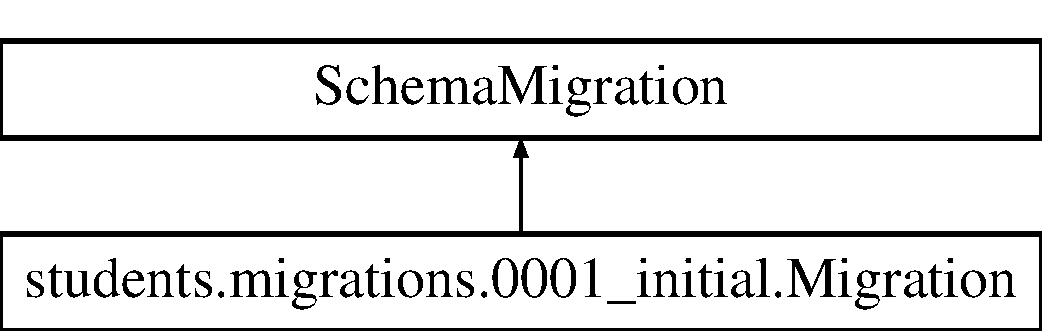
\includegraphics[height=2.000000cm]{classstudents_1_1migrations_1_10001__initial_1_1_migration}
\end{center}
\end{figure}
\subsection*{Public Member Functions}
\begin{DoxyCompactItemize}
\item 
def \hyperlink{classstudents_1_1migrations_1_10001__initial_1_1_migration_a87a94afad1b7e38c614de2d8c945ffb6}{forwards}
\item 
def \hyperlink{classstudents_1_1migrations_1_10001__initial_1_1_migration_a0bef6d594d4301d31809f74f12b4b765}{backwards}
\end{DoxyCompactItemize}
\subsection*{Static Public Attributes}
\begin{DoxyCompactItemize}
\item 
dictionary \hyperlink{classstudents_1_1migrations_1_10001__initial_1_1_migration_a6bf5c96d511e88a3ab94d17c1e40434f}{models}
\end{DoxyCompactItemize}


\subsection{Member Function Documentation}
\hypertarget{classstudents_1_1migrations_1_10001__initial_1_1_migration_a0bef6d594d4301d31809f74f12b4b765}{\index{students\-::migrations\-::0001\-\_\-initial\-::\-Migration@{students\-::migrations\-::0001\-\_\-initial\-::\-Migration}!backwards@{backwards}}
\index{backwards@{backwards}!students::migrations::0001_initial::Migration@{students\-::migrations\-::0001\-\_\-initial\-::\-Migration}}
\subsubsection[{backwards}]{\setlength{\rightskip}{0pt plus 5cm}def students.\-migrations.\-0001\-\_\-initial.\-Migration.\-backwards (
\begin{DoxyParamCaption}
\item[{}]{self, }
\item[{}]{orm}
\end{DoxyParamCaption}
)}}\label{classstudents_1_1migrations_1_10001__initial_1_1_migration_a0bef6d594d4301d31809f74f12b4b765}
\hypertarget{classstudents_1_1migrations_1_10001__initial_1_1_migration_a87a94afad1b7e38c614de2d8c945ffb6}{\index{students\-::migrations\-::0001\-\_\-initial\-::\-Migration@{students\-::migrations\-::0001\-\_\-initial\-::\-Migration}!forwards@{forwards}}
\index{forwards@{forwards}!students::migrations::0001_initial::Migration@{students\-::migrations\-::0001\-\_\-initial\-::\-Migration}}
\subsubsection[{forwards}]{\setlength{\rightskip}{0pt plus 5cm}def students.\-migrations.\-0001\-\_\-initial.\-Migration.\-forwards (
\begin{DoxyParamCaption}
\item[{}]{self, }
\item[{}]{orm}
\end{DoxyParamCaption}
)}}\label{classstudents_1_1migrations_1_10001__initial_1_1_migration_a87a94afad1b7e38c614de2d8c945ffb6}


\subsection{Member Data Documentation}
\hypertarget{classstudents_1_1migrations_1_10001__initial_1_1_migration_a6bf5c96d511e88a3ab94d17c1e40434f}{\index{students\-::migrations\-::0001\-\_\-initial\-::\-Migration@{students\-::migrations\-::0001\-\_\-initial\-::\-Migration}!models@{models}}
\index{models@{models}!students::migrations::0001_initial::Migration@{students\-::migrations\-::0001\-\_\-initial\-::\-Migration}}
\subsubsection[{models}]{\setlength{\rightskip}{0pt plus 5cm}dictionary students.\-migrations.\-0001\-\_\-initial.\-Migration.\-models\hspace{0.3cm}{\ttfamily [static]}}}\label{classstudents_1_1migrations_1_10001__initial_1_1_migration_a6bf5c96d511e88a3ab94d17c1e40434f}


The documentation for this class was generated from the following file\-:\begin{DoxyCompactItemize}
\item 
leapkit/students/migrations/\hyperlink{0001__initial_8py}{0001\-\_\-initial.\-py}\end{DoxyCompactItemize}

\hypertarget{classstudents_1_1migrations_1_10002__auto____add__field__student__cv_1_1_migration}{\section{students.\-migrations.0002\-\_\-auto\-\_\-\-\_\-add\-\_\-field\-\_\-student\-\_\-cv.Migration Class Reference}
\label{classstudents_1_1migrations_1_10002__auto____add__field__student__cv_1_1_migration}\index{students.\-migrations.\-0002\-\_\-auto\-\_\-\-\_\-add\-\_\-field\-\_\-student\-\_\-cv.\-Migration@{students.\-migrations.\-0002\-\_\-auto\-\_\-\-\_\-add\-\_\-field\-\_\-student\-\_\-cv.\-Migration}}
}
Inheritance diagram for students.\-migrations.0002\-\_\-auto\-\_\-\-\_\-add\-\_\-field\-\_\-student\-\_\-cv.Migration\-:\begin{figure}[H]
\begin{center}
\leavevmode
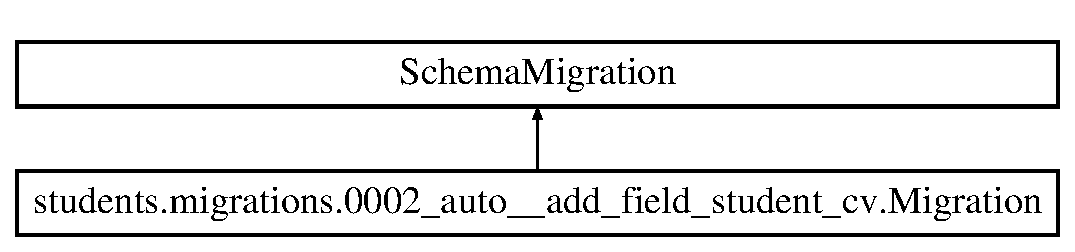
\includegraphics[height=2.000000cm]{classstudents_1_1migrations_1_10002__auto____add__field__student__cv_1_1_migration}
\end{center}
\end{figure}
\subsection*{Public Member Functions}
\begin{DoxyCompactItemize}
\item 
def \hyperlink{classstudents_1_1migrations_1_10002__auto____add__field__student__cv_1_1_migration_a9a923d2d1ae804311fa0803b468b8f4b}{forwards}
\item 
def \hyperlink{classstudents_1_1migrations_1_10002__auto____add__field__student__cv_1_1_migration_ae492244bf15cb25ccf6aaec16e6629a9}{backwards}
\end{DoxyCompactItemize}
\subsection*{Static Public Attributes}
\begin{DoxyCompactItemize}
\item 
dictionary \hyperlink{classstudents_1_1migrations_1_10002__auto____add__field__student__cv_1_1_migration_a341e15c4f0ea5a07c66d93d02d3fb464}{models}
\end{DoxyCompactItemize}


\subsection{Member Function Documentation}
\hypertarget{classstudents_1_1migrations_1_10002__auto____add__field__student__cv_1_1_migration_ae492244bf15cb25ccf6aaec16e6629a9}{\index{students\-::migrations\-::0002\-\_\-auto\-\_\-\-\_\-add\-\_\-field\-\_\-student\-\_\-cv\-::\-Migration@{students\-::migrations\-::0002\-\_\-auto\-\_\-\-\_\-add\-\_\-field\-\_\-student\-\_\-cv\-::\-Migration}!backwards@{backwards}}
\index{backwards@{backwards}!students::migrations::0002_auto__add_field_student_cv::Migration@{students\-::migrations\-::0002\-\_\-auto\-\_\-\-\_\-add\-\_\-field\-\_\-student\-\_\-cv\-::\-Migration}}
\subsubsection[{backwards}]{\setlength{\rightskip}{0pt plus 5cm}def students.\-migrations.\-0002\-\_\-auto\-\_\-\-\_\-add\-\_\-field\-\_\-student\-\_\-cv.\-Migration.\-backwards (
\begin{DoxyParamCaption}
\item[{}]{self, }
\item[{}]{orm}
\end{DoxyParamCaption}
)}}\label{classstudents_1_1migrations_1_10002__auto____add__field__student__cv_1_1_migration_ae492244bf15cb25ccf6aaec16e6629a9}
\hypertarget{classstudents_1_1migrations_1_10002__auto____add__field__student__cv_1_1_migration_a9a923d2d1ae804311fa0803b468b8f4b}{\index{students\-::migrations\-::0002\-\_\-auto\-\_\-\-\_\-add\-\_\-field\-\_\-student\-\_\-cv\-::\-Migration@{students\-::migrations\-::0002\-\_\-auto\-\_\-\-\_\-add\-\_\-field\-\_\-student\-\_\-cv\-::\-Migration}!forwards@{forwards}}
\index{forwards@{forwards}!students::migrations::0002_auto__add_field_student_cv::Migration@{students\-::migrations\-::0002\-\_\-auto\-\_\-\-\_\-add\-\_\-field\-\_\-student\-\_\-cv\-::\-Migration}}
\subsubsection[{forwards}]{\setlength{\rightskip}{0pt plus 5cm}def students.\-migrations.\-0002\-\_\-auto\-\_\-\-\_\-add\-\_\-field\-\_\-student\-\_\-cv.\-Migration.\-forwards (
\begin{DoxyParamCaption}
\item[{}]{self, }
\item[{}]{orm}
\end{DoxyParamCaption}
)}}\label{classstudents_1_1migrations_1_10002__auto____add__field__student__cv_1_1_migration_a9a923d2d1ae804311fa0803b468b8f4b}


\subsection{Member Data Documentation}
\hypertarget{classstudents_1_1migrations_1_10002__auto____add__field__student__cv_1_1_migration_a341e15c4f0ea5a07c66d93d02d3fb464}{\index{students\-::migrations\-::0002\-\_\-auto\-\_\-\-\_\-add\-\_\-field\-\_\-student\-\_\-cv\-::\-Migration@{students\-::migrations\-::0002\-\_\-auto\-\_\-\-\_\-add\-\_\-field\-\_\-student\-\_\-cv\-::\-Migration}!models@{models}}
\index{models@{models}!students::migrations::0002_auto__add_field_student_cv::Migration@{students\-::migrations\-::0002\-\_\-auto\-\_\-\-\_\-add\-\_\-field\-\_\-student\-\_\-cv\-::\-Migration}}
\subsubsection[{models}]{\setlength{\rightskip}{0pt plus 5cm}dictionary students.\-migrations.\-0002\-\_\-auto\-\_\-\-\_\-add\-\_\-field\-\_\-student\-\_\-cv.\-Migration.\-models\hspace{0.3cm}{\ttfamily [static]}}}\label{classstudents_1_1migrations_1_10002__auto____add__field__student__cv_1_1_migration_a341e15c4f0ea5a07c66d93d02d3fb464}


The documentation for this class was generated from the following file\-:\begin{DoxyCompactItemize}
\item 
leapkit/students/migrations/\hyperlink{0002__auto____add__field__student__cv_8py}{0002\-\_\-auto\-\_\-\-\_\-add\-\_\-field\-\_\-student\-\_\-cv.\-py}\end{DoxyCompactItemize}

\hypertarget{classstudents_1_1migrations_1_10003__auto____add__field__student__line__of__study_1_1_migration}{\section{students.\-migrations.0003\-\_\-auto\-\_\-\-\_\-add\-\_\-field\-\_\-student\-\_\-line\-\_\-of\-\_\-study.Migration Class Reference}
\label{classstudents_1_1migrations_1_10003__auto____add__field__student__line__of__study_1_1_migration}\index{students.\-migrations.\-0003\-\_\-auto\-\_\-\-\_\-add\-\_\-field\-\_\-student\-\_\-line\-\_\-of\-\_\-study.\-Migration@{students.\-migrations.\-0003\-\_\-auto\-\_\-\-\_\-add\-\_\-field\-\_\-student\-\_\-line\-\_\-of\-\_\-study.\-Migration}}
}
Inheritance diagram for students.\-migrations.0003\-\_\-auto\-\_\-\-\_\-add\-\_\-field\-\_\-student\-\_\-line\-\_\-of\-\_\-study.Migration\-:\begin{figure}[H]
\begin{center}
\leavevmode
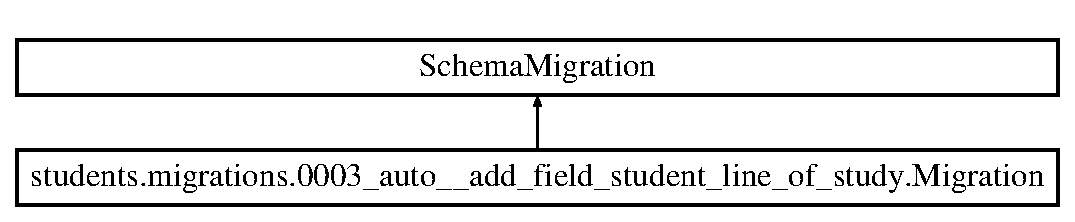
\includegraphics[height=2.000000cm]{classstudents_1_1migrations_1_10003__auto____add__field__student__line__of__study_1_1_migration}
\end{center}
\end{figure}
\subsection*{Public Member Functions}
\begin{DoxyCompactItemize}
\item 
def \hyperlink{classstudents_1_1migrations_1_10003__auto____add__field__student__line__of__study_1_1_migration_a94a867dd97a643482e02f5e9598f213f}{forwards}
\item 
def \hyperlink{classstudents_1_1migrations_1_10003__auto____add__field__student__line__of__study_1_1_migration_af6244739d0541193d6658b834716c9ea}{backwards}
\end{DoxyCompactItemize}
\subsection*{Static Public Attributes}
\begin{DoxyCompactItemize}
\item 
dictionary \hyperlink{classstudents_1_1migrations_1_10003__auto____add__field__student__line__of__study_1_1_migration_a1656f729c63dfbc632ab6070a4d7a813}{models}
\end{DoxyCompactItemize}


\subsection{Member Function Documentation}
\hypertarget{classstudents_1_1migrations_1_10003__auto____add__field__student__line__of__study_1_1_migration_af6244739d0541193d6658b834716c9ea}{\index{students\-::migrations\-::0003\-\_\-auto\-\_\-\-\_\-add\-\_\-field\-\_\-student\-\_\-line\-\_\-of\-\_\-study\-::\-Migration@{students\-::migrations\-::0003\-\_\-auto\-\_\-\-\_\-add\-\_\-field\-\_\-student\-\_\-line\-\_\-of\-\_\-study\-::\-Migration}!backwards@{backwards}}
\index{backwards@{backwards}!students::migrations::0003_auto__add_field_student_line_of_study::Migration@{students\-::migrations\-::0003\-\_\-auto\-\_\-\-\_\-add\-\_\-field\-\_\-student\-\_\-line\-\_\-of\-\_\-study\-::\-Migration}}
\subsubsection[{backwards}]{\setlength{\rightskip}{0pt plus 5cm}def students.\-migrations.\-0003\-\_\-auto\-\_\-\-\_\-add\-\_\-field\-\_\-student\-\_\-line\-\_\-of\-\_\-study.\-Migration.\-backwards (
\begin{DoxyParamCaption}
\item[{}]{self, }
\item[{}]{orm}
\end{DoxyParamCaption}
)}}\label{classstudents_1_1migrations_1_10003__auto____add__field__student__line__of__study_1_1_migration_af6244739d0541193d6658b834716c9ea}
\hypertarget{classstudents_1_1migrations_1_10003__auto____add__field__student__line__of__study_1_1_migration_a94a867dd97a643482e02f5e9598f213f}{\index{students\-::migrations\-::0003\-\_\-auto\-\_\-\-\_\-add\-\_\-field\-\_\-student\-\_\-line\-\_\-of\-\_\-study\-::\-Migration@{students\-::migrations\-::0003\-\_\-auto\-\_\-\-\_\-add\-\_\-field\-\_\-student\-\_\-line\-\_\-of\-\_\-study\-::\-Migration}!forwards@{forwards}}
\index{forwards@{forwards}!students::migrations::0003_auto__add_field_student_line_of_study::Migration@{students\-::migrations\-::0003\-\_\-auto\-\_\-\-\_\-add\-\_\-field\-\_\-student\-\_\-line\-\_\-of\-\_\-study\-::\-Migration}}
\subsubsection[{forwards}]{\setlength{\rightskip}{0pt plus 5cm}def students.\-migrations.\-0003\-\_\-auto\-\_\-\-\_\-add\-\_\-field\-\_\-student\-\_\-line\-\_\-of\-\_\-study.\-Migration.\-forwards (
\begin{DoxyParamCaption}
\item[{}]{self, }
\item[{}]{orm}
\end{DoxyParamCaption}
)}}\label{classstudents_1_1migrations_1_10003__auto____add__field__student__line__of__study_1_1_migration_a94a867dd97a643482e02f5e9598f213f}


\subsection{Member Data Documentation}
\hypertarget{classstudents_1_1migrations_1_10003__auto____add__field__student__line__of__study_1_1_migration_a1656f729c63dfbc632ab6070a4d7a813}{\index{students\-::migrations\-::0003\-\_\-auto\-\_\-\-\_\-add\-\_\-field\-\_\-student\-\_\-line\-\_\-of\-\_\-study\-::\-Migration@{students\-::migrations\-::0003\-\_\-auto\-\_\-\-\_\-add\-\_\-field\-\_\-student\-\_\-line\-\_\-of\-\_\-study\-::\-Migration}!models@{models}}
\index{models@{models}!students::migrations::0003_auto__add_field_student_line_of_study::Migration@{students\-::migrations\-::0003\-\_\-auto\-\_\-\-\_\-add\-\_\-field\-\_\-student\-\_\-line\-\_\-of\-\_\-study\-::\-Migration}}
\subsubsection[{models}]{\setlength{\rightskip}{0pt plus 5cm}dictionary students.\-migrations.\-0003\-\_\-auto\-\_\-\-\_\-add\-\_\-field\-\_\-student\-\_\-line\-\_\-of\-\_\-study.\-Migration.\-models\hspace{0.3cm}{\ttfamily [static]}}}\label{classstudents_1_1migrations_1_10003__auto____add__field__student__line__of__study_1_1_migration_a1656f729c63dfbc632ab6070a4d7a813}


The documentation for this class was generated from the following file\-:\begin{DoxyCompactItemize}
\item 
leapkit/students/migrations/\hyperlink{0003__auto____add__field__student__line__of__study_8py}{0003\-\_\-auto\-\_\-\-\_\-add\-\_\-field\-\_\-student\-\_\-line\-\_\-of\-\_\-study.\-py}\end{DoxyCompactItemize}

\hypertarget{classstudents_1_1migrations_1_10004__auto____add__field__student__education__level_1_1_migration}{\section{students.\-migrations.0004\-\_\-auto\-\_\-\-\_\-add\-\_\-field\-\_\-student\-\_\-education\-\_\-level.Migration Class Reference}
\label{classstudents_1_1migrations_1_10004__auto____add__field__student__education__level_1_1_migration}\index{students.\-migrations.\-0004\-\_\-auto\-\_\-\-\_\-add\-\_\-field\-\_\-student\-\_\-education\-\_\-level.\-Migration@{students.\-migrations.\-0004\-\_\-auto\-\_\-\-\_\-add\-\_\-field\-\_\-student\-\_\-education\-\_\-level.\-Migration}}
}
Inheritance diagram for students.\-migrations.0004\-\_\-auto\-\_\-\-\_\-add\-\_\-field\-\_\-student\-\_\-education\-\_\-level.Migration\-:\begin{figure}[H]
\begin{center}
\leavevmode
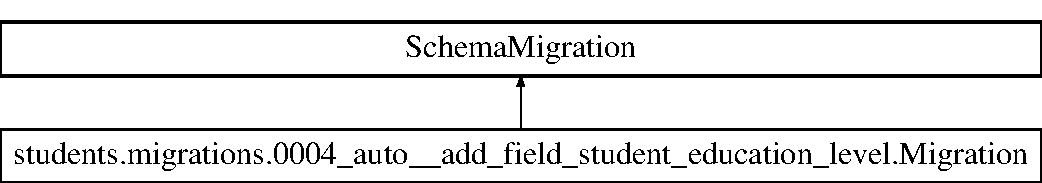
\includegraphics[height=2.000000cm]{classstudents_1_1migrations_1_10004__auto____add__field__student__education__level_1_1_migration}
\end{center}
\end{figure}
\subsection*{Public Member Functions}
\begin{DoxyCompactItemize}
\item 
def \hyperlink{classstudents_1_1migrations_1_10004__auto____add__field__student__education__level_1_1_migration_a943692e13dee282cb162e64d0c0b268b}{forwards}
\item 
def \hyperlink{classstudents_1_1migrations_1_10004__auto____add__field__student__education__level_1_1_migration_a24114a5c2f9de7676ba5e5d8fc70406c}{backwards}
\end{DoxyCompactItemize}
\subsection*{Static Public Attributes}
\begin{DoxyCompactItemize}
\item 
dictionary \hyperlink{classstudents_1_1migrations_1_10004__auto____add__field__student__education__level_1_1_migration_a52c034bfca3afbfe91f1d98ee4690657}{models}
\end{DoxyCompactItemize}


\subsection{Member Function Documentation}
\hypertarget{classstudents_1_1migrations_1_10004__auto____add__field__student__education__level_1_1_migration_a24114a5c2f9de7676ba5e5d8fc70406c}{\index{students\-::migrations\-::0004\-\_\-auto\-\_\-\-\_\-add\-\_\-field\-\_\-student\-\_\-education\-\_\-level\-::\-Migration@{students\-::migrations\-::0004\-\_\-auto\-\_\-\-\_\-add\-\_\-field\-\_\-student\-\_\-education\-\_\-level\-::\-Migration}!backwards@{backwards}}
\index{backwards@{backwards}!students::migrations::0004_auto__add_field_student_education_level::Migration@{students\-::migrations\-::0004\-\_\-auto\-\_\-\-\_\-add\-\_\-field\-\_\-student\-\_\-education\-\_\-level\-::\-Migration}}
\subsubsection[{backwards}]{\setlength{\rightskip}{0pt plus 5cm}def students.\-migrations.\-0004\-\_\-auto\-\_\-\-\_\-add\-\_\-field\-\_\-student\-\_\-education\-\_\-level.\-Migration.\-backwards (
\begin{DoxyParamCaption}
\item[{}]{self, }
\item[{}]{orm}
\end{DoxyParamCaption}
)}}\label{classstudents_1_1migrations_1_10004__auto____add__field__student__education__level_1_1_migration_a24114a5c2f9de7676ba5e5d8fc70406c}
\hypertarget{classstudents_1_1migrations_1_10004__auto____add__field__student__education__level_1_1_migration_a943692e13dee282cb162e64d0c0b268b}{\index{students\-::migrations\-::0004\-\_\-auto\-\_\-\-\_\-add\-\_\-field\-\_\-student\-\_\-education\-\_\-level\-::\-Migration@{students\-::migrations\-::0004\-\_\-auto\-\_\-\-\_\-add\-\_\-field\-\_\-student\-\_\-education\-\_\-level\-::\-Migration}!forwards@{forwards}}
\index{forwards@{forwards}!students::migrations::0004_auto__add_field_student_education_level::Migration@{students\-::migrations\-::0004\-\_\-auto\-\_\-\-\_\-add\-\_\-field\-\_\-student\-\_\-education\-\_\-level\-::\-Migration}}
\subsubsection[{forwards}]{\setlength{\rightskip}{0pt plus 5cm}def students.\-migrations.\-0004\-\_\-auto\-\_\-\-\_\-add\-\_\-field\-\_\-student\-\_\-education\-\_\-level.\-Migration.\-forwards (
\begin{DoxyParamCaption}
\item[{}]{self, }
\item[{}]{orm}
\end{DoxyParamCaption}
)}}\label{classstudents_1_1migrations_1_10004__auto____add__field__student__education__level_1_1_migration_a943692e13dee282cb162e64d0c0b268b}


\subsection{Member Data Documentation}
\hypertarget{classstudents_1_1migrations_1_10004__auto____add__field__student__education__level_1_1_migration_a52c034bfca3afbfe91f1d98ee4690657}{\index{students\-::migrations\-::0004\-\_\-auto\-\_\-\-\_\-add\-\_\-field\-\_\-student\-\_\-education\-\_\-level\-::\-Migration@{students\-::migrations\-::0004\-\_\-auto\-\_\-\-\_\-add\-\_\-field\-\_\-student\-\_\-education\-\_\-level\-::\-Migration}!models@{models}}
\index{models@{models}!students::migrations::0004_auto__add_field_student_education_level::Migration@{students\-::migrations\-::0004\-\_\-auto\-\_\-\-\_\-add\-\_\-field\-\_\-student\-\_\-education\-\_\-level\-::\-Migration}}
\subsubsection[{models}]{\setlength{\rightskip}{0pt plus 5cm}dictionary students.\-migrations.\-0004\-\_\-auto\-\_\-\-\_\-add\-\_\-field\-\_\-student\-\_\-education\-\_\-level.\-Migration.\-models\hspace{0.3cm}{\ttfamily [static]}}}\label{classstudents_1_1migrations_1_10004__auto____add__field__student__education__level_1_1_migration_a52c034bfca3afbfe91f1d98ee4690657}


The documentation for this class was generated from the following file\-:\begin{DoxyCompactItemize}
\item 
leapkit/students/migrations/\hyperlink{0004__auto____add__field__student__education__level_8py}{0004\-\_\-auto\-\_\-\-\_\-add\-\_\-field\-\_\-student\-\_\-education\-\_\-level.\-py}\end{DoxyCompactItemize}

\hypertarget{classstudents_1_1migrations_1_10005__auto____add__field__student__times__logged__in_1_1_migration}{\section{students.\-migrations.0005\-\_\-auto\-\_\-\-\_\-add\-\_\-field\-\_\-student\-\_\-times\-\_\-logged\-\_\-in.Migration Class Reference}
\label{classstudents_1_1migrations_1_10005__auto____add__field__student__times__logged__in_1_1_migration}\index{students.\-migrations.\-0005\-\_\-auto\-\_\-\-\_\-add\-\_\-field\-\_\-student\-\_\-times\-\_\-logged\-\_\-in.\-Migration@{students.\-migrations.\-0005\-\_\-auto\-\_\-\-\_\-add\-\_\-field\-\_\-student\-\_\-times\-\_\-logged\-\_\-in.\-Migration}}
}
Inheritance diagram for students.\-migrations.0005\-\_\-auto\-\_\-\-\_\-add\-\_\-field\-\_\-student\-\_\-times\-\_\-logged\-\_\-in.Migration\-:\begin{figure}[H]
\begin{center}
\leavevmode
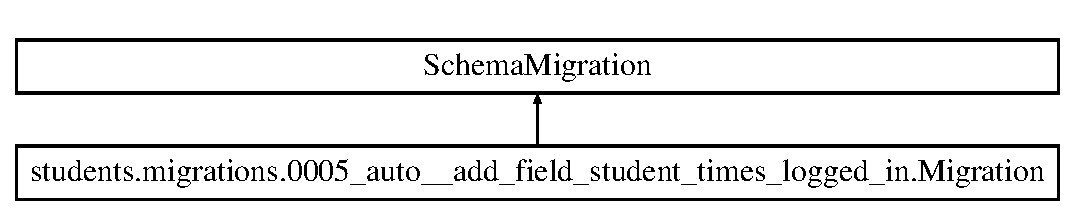
\includegraphics[height=2.000000cm]{classstudents_1_1migrations_1_10005__auto____add__field__student__times__logged__in_1_1_migration}
\end{center}
\end{figure}
\subsection*{Public Member Functions}
\begin{DoxyCompactItemize}
\item 
def \hyperlink{classstudents_1_1migrations_1_10005__auto____add__field__student__times__logged__in_1_1_migration_aefa02ac46c43ced3f3cd7b9551660e8f}{forwards}
\item 
def \hyperlink{classstudents_1_1migrations_1_10005__auto____add__field__student__times__logged__in_1_1_migration_a14280cab7177a420441ed1e484422d97}{backwards}
\end{DoxyCompactItemize}
\subsection*{Static Public Attributes}
\begin{DoxyCompactItemize}
\item 
dictionary \hyperlink{classstudents_1_1migrations_1_10005__auto____add__field__student__times__logged__in_1_1_migration_aa96b2fe7dad0ea621ed20c777dcfdbcc}{models}
\end{DoxyCompactItemize}


\subsection{Member Function Documentation}
\hypertarget{classstudents_1_1migrations_1_10005__auto____add__field__student__times__logged__in_1_1_migration_a14280cab7177a420441ed1e484422d97}{\index{students\-::migrations\-::0005\-\_\-auto\-\_\-\-\_\-add\-\_\-field\-\_\-student\-\_\-times\-\_\-logged\-\_\-in\-::\-Migration@{students\-::migrations\-::0005\-\_\-auto\-\_\-\-\_\-add\-\_\-field\-\_\-student\-\_\-times\-\_\-logged\-\_\-in\-::\-Migration}!backwards@{backwards}}
\index{backwards@{backwards}!students::migrations::0005_auto__add_field_student_times_logged_in::Migration@{students\-::migrations\-::0005\-\_\-auto\-\_\-\-\_\-add\-\_\-field\-\_\-student\-\_\-times\-\_\-logged\-\_\-in\-::\-Migration}}
\subsubsection[{backwards}]{\setlength{\rightskip}{0pt plus 5cm}def students.\-migrations.\-0005\-\_\-auto\-\_\-\-\_\-add\-\_\-field\-\_\-student\-\_\-times\-\_\-logged\-\_\-in.\-Migration.\-backwards (
\begin{DoxyParamCaption}
\item[{}]{self, }
\item[{}]{orm}
\end{DoxyParamCaption}
)}}\label{classstudents_1_1migrations_1_10005__auto____add__field__student__times__logged__in_1_1_migration_a14280cab7177a420441ed1e484422d97}
\hypertarget{classstudents_1_1migrations_1_10005__auto____add__field__student__times__logged__in_1_1_migration_aefa02ac46c43ced3f3cd7b9551660e8f}{\index{students\-::migrations\-::0005\-\_\-auto\-\_\-\-\_\-add\-\_\-field\-\_\-student\-\_\-times\-\_\-logged\-\_\-in\-::\-Migration@{students\-::migrations\-::0005\-\_\-auto\-\_\-\-\_\-add\-\_\-field\-\_\-student\-\_\-times\-\_\-logged\-\_\-in\-::\-Migration}!forwards@{forwards}}
\index{forwards@{forwards}!students::migrations::0005_auto__add_field_student_times_logged_in::Migration@{students\-::migrations\-::0005\-\_\-auto\-\_\-\-\_\-add\-\_\-field\-\_\-student\-\_\-times\-\_\-logged\-\_\-in\-::\-Migration}}
\subsubsection[{forwards}]{\setlength{\rightskip}{0pt plus 5cm}def students.\-migrations.\-0005\-\_\-auto\-\_\-\-\_\-add\-\_\-field\-\_\-student\-\_\-times\-\_\-logged\-\_\-in.\-Migration.\-forwards (
\begin{DoxyParamCaption}
\item[{}]{self, }
\item[{}]{orm}
\end{DoxyParamCaption}
)}}\label{classstudents_1_1migrations_1_10005__auto____add__field__student__times__logged__in_1_1_migration_aefa02ac46c43ced3f3cd7b9551660e8f}


\subsection{Member Data Documentation}
\hypertarget{classstudents_1_1migrations_1_10005__auto____add__field__student__times__logged__in_1_1_migration_aa96b2fe7dad0ea621ed20c777dcfdbcc}{\index{students\-::migrations\-::0005\-\_\-auto\-\_\-\-\_\-add\-\_\-field\-\_\-student\-\_\-times\-\_\-logged\-\_\-in\-::\-Migration@{students\-::migrations\-::0005\-\_\-auto\-\_\-\-\_\-add\-\_\-field\-\_\-student\-\_\-times\-\_\-logged\-\_\-in\-::\-Migration}!models@{models}}
\index{models@{models}!students::migrations::0005_auto__add_field_student_times_logged_in::Migration@{students\-::migrations\-::0005\-\_\-auto\-\_\-\-\_\-add\-\_\-field\-\_\-student\-\_\-times\-\_\-logged\-\_\-in\-::\-Migration}}
\subsubsection[{models}]{\setlength{\rightskip}{0pt plus 5cm}dictionary students.\-migrations.\-0005\-\_\-auto\-\_\-\-\_\-add\-\_\-field\-\_\-student\-\_\-times\-\_\-logged\-\_\-in.\-Migration.\-models\hspace{0.3cm}{\ttfamily [static]}}}\label{classstudents_1_1migrations_1_10005__auto____add__field__student__times__logged__in_1_1_migration_aa96b2fe7dad0ea621ed20c777dcfdbcc}


The documentation for this class was generated from the following file\-:\begin{DoxyCompactItemize}
\item 
leapkit/students/migrations/\hyperlink{0005__auto____add__field__student__times__logged__in_8py}{0005\-\_\-auto\-\_\-\-\_\-add\-\_\-field\-\_\-student\-\_\-times\-\_\-logged\-\_\-in.\-py}\end{DoxyCompactItemize}

\hypertarget{classstudents_1_1linkedin__converter_1_1_person}{\section{students.\-linkedin\-\_\-converter.\-Person Class Reference}
\label{classstudents_1_1linkedin__converter_1_1_person}\index{students.\-linkedin\-\_\-converter.\-Person@{students.\-linkedin\-\_\-converter.\-Person}}
}


Data Structure \#\#.  


Inheritance diagram for students.\-linkedin\-\_\-converter.\-Person\-:\begin{figure}[H]
\begin{center}
\leavevmode
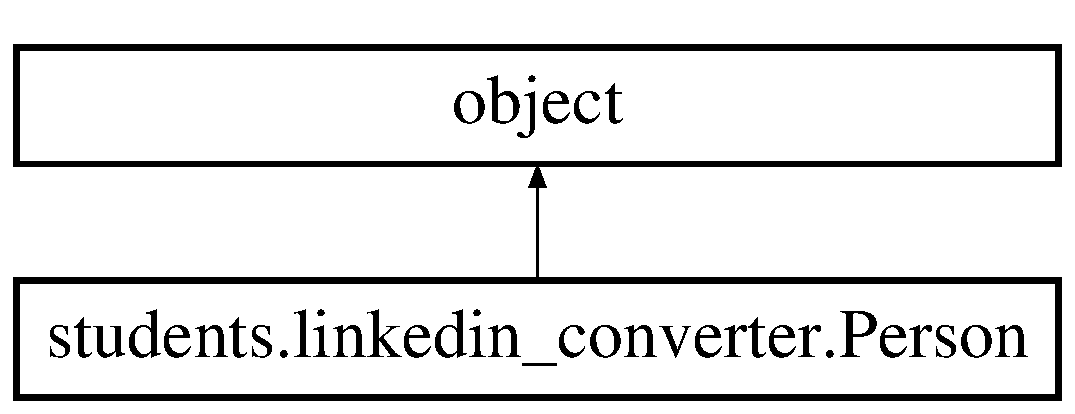
\includegraphics[height=2.000000cm]{classstudents_1_1linkedin__converter_1_1_person}
\end{center}
\end{figure}
\subsection*{Public Member Functions}
\begin{DoxyCompactItemize}
\item 
def \hyperlink{classstudents_1_1linkedin__converter_1_1_person_a76d56276758c7b0e878fddb0d2653db2}{\-\_\-\-\_\-str\-\_\-\-\_\-}
\end{DoxyCompactItemize}
\subsection*{Static Public Attributes}
\begin{DoxyCompactItemize}
\item 
string \hyperlink{classstudents_1_1linkedin__converter_1_1_person_a65beb2ae251f6c6e654ad25792281894}{pid} = \char`\"{}\char`\"{}
\item 
string \hyperlink{classstudents_1_1linkedin__converter_1_1_person_a35d5d60ceec03ba305e8a189db380ac2}{first\-Name} = \char`\"{}\char`\"{}
\item 
string \hyperlink{classstudents_1_1linkedin__converter_1_1_person_a3df0a3de068edad635f12d079457eb6b}{maiden\-Name} = \char`\"{}\char`\"{}
\item 
string \hyperlink{classstudents_1_1linkedin__converter_1_1_person_a2d040eac8e8b47f0e6c38b0bfab76b55}{last\-Name} = \char`\"{}\char`\"{}
\item 
string \hyperlink{classstudents_1_1linkedin__converter_1_1_person_acfa2c2248119cc7a9ffac6d4b96bc57b}{location} = \char`\"{}\char`\"{}
\item 
string \hyperlink{classstudents_1_1linkedin__converter_1_1_person_acd8938604a06b662b9b1445ccf359755}{specialities} = \char`\"{}\char`\"{}
\item 
string \hyperlink{classstudents_1_1linkedin__converter_1_1_person_a63b0f5ecae1b9140534919b8fc603e81}{picture\-Url} = \char`\"{}\char`\"{}
\item 
string \hyperlink{classstudents_1_1linkedin__converter_1_1_person_aea14e8c81d34be3e77329b05de1a24b1}{public\-Profile\-Url} = \char`\"{}\char`\"{}
\item 
list \hyperlink{classstudents_1_1linkedin__converter_1_1_person_a1b395c681cf806d60dc98eaf3a3d9f8d}{positions} = \mbox{[}$\,$\mbox{]}
\item 
list \hyperlink{classstudents_1_1linkedin__converter_1_1_person_a9e7d26cf8c69ccb6bb34e6c5c8dc0873}{skills} = \mbox{[}$\,$\mbox{]}
\item 
list \hyperlink{classstudents_1_1linkedin__converter_1_1_person_a5cfb1cc9dbb197b1e5452007119a7afd}{educations} = \mbox{[}$\,$\mbox{]}
\item 
list \hyperlink{classstudents_1_1linkedin__converter_1_1_person_ada2e4be2ab676d1723df1ef723ce6ace}{courses} = \mbox{[}$\,$\mbox{]}
\item 
list \hyperlink{classstudents_1_1linkedin__converter_1_1_person_a564e0fd67ce9e7d2fe1c77badcd54575}{languages} = \mbox{[}$\,$\mbox{]}
\end{DoxyCompactItemize}


\subsection{Detailed Description}
Data Structure \#\#. 

\begin{DoxyVerb}A person is used to structure a json string\end{DoxyVerb}
 \begin{DoxyVerb}Constructor that initiates all the basic person values\end{DoxyVerb}
 

\subsection{Member Function Documentation}
\hypertarget{classstudents_1_1linkedin__converter_1_1_person_a76d56276758c7b0e878fddb0d2653db2}{\index{students\-::linkedin\-\_\-converter\-::\-Person@{students\-::linkedin\-\_\-converter\-::\-Person}!\-\_\-\-\_\-str\-\_\-\-\_\-@{\-\_\-\-\_\-str\-\_\-\-\_\-}}
\index{\-\_\-\-\_\-str\-\_\-\-\_\-@{\-\_\-\-\_\-str\-\_\-\-\_\-}!students::linkedin_converter::Person@{students\-::linkedin\-\_\-converter\-::\-Person}}
\subsubsection[{\-\_\-\-\_\-str\-\_\-\-\_\-}]{\setlength{\rightskip}{0pt plus 5cm}def students.\-linkedin\-\_\-converter.\-Person.\-\_\-\-\_\-str\-\_\-\-\_\- (
\begin{DoxyParamCaption}
\item[{}]{self}
\end{DoxyParamCaption}
)}}\label{classstudents_1_1linkedin__converter_1_1_person_a76d56276758c7b0e878fddb0d2653db2}
\begin{DoxyVerb}Returns a string with all information from that user\end{DoxyVerb}
 

\subsection{Member Data Documentation}
\hypertarget{classstudents_1_1linkedin__converter_1_1_person_ada2e4be2ab676d1723df1ef723ce6ace}{\index{students\-::linkedin\-\_\-converter\-::\-Person@{students\-::linkedin\-\_\-converter\-::\-Person}!courses@{courses}}
\index{courses@{courses}!students::linkedin_converter::Person@{students\-::linkedin\-\_\-converter\-::\-Person}}
\subsubsection[{courses}]{\setlength{\rightskip}{0pt plus 5cm}list students.\-linkedin\-\_\-converter.\-Person.\-courses = \mbox{[}$\,$\mbox{]}\hspace{0.3cm}{\ttfamily [static]}}}\label{classstudents_1_1linkedin__converter_1_1_person_ada2e4be2ab676d1723df1ef723ce6ace}
\hypertarget{classstudents_1_1linkedin__converter_1_1_person_a5cfb1cc9dbb197b1e5452007119a7afd}{\index{students\-::linkedin\-\_\-converter\-::\-Person@{students\-::linkedin\-\_\-converter\-::\-Person}!educations@{educations}}
\index{educations@{educations}!students::linkedin_converter::Person@{students\-::linkedin\-\_\-converter\-::\-Person}}
\subsubsection[{educations}]{\setlength{\rightskip}{0pt plus 5cm}list students.\-linkedin\-\_\-converter.\-Person.\-educations = \mbox{[}$\,$\mbox{]}\hspace{0.3cm}{\ttfamily [static]}}}\label{classstudents_1_1linkedin__converter_1_1_person_a5cfb1cc9dbb197b1e5452007119a7afd}
\hypertarget{classstudents_1_1linkedin__converter_1_1_person_a35d5d60ceec03ba305e8a189db380ac2}{\index{students\-::linkedin\-\_\-converter\-::\-Person@{students\-::linkedin\-\_\-converter\-::\-Person}!first\-Name@{first\-Name}}
\index{first\-Name@{first\-Name}!students::linkedin_converter::Person@{students\-::linkedin\-\_\-converter\-::\-Person}}
\subsubsection[{first\-Name}]{\setlength{\rightskip}{0pt plus 5cm}string students.\-linkedin\-\_\-converter.\-Person.\-first\-Name = \char`\"{}\char`\"{}\hspace{0.3cm}{\ttfamily [static]}}}\label{classstudents_1_1linkedin__converter_1_1_person_a35d5d60ceec03ba305e8a189db380ac2}
\hypertarget{classstudents_1_1linkedin__converter_1_1_person_a564e0fd67ce9e7d2fe1c77badcd54575}{\index{students\-::linkedin\-\_\-converter\-::\-Person@{students\-::linkedin\-\_\-converter\-::\-Person}!languages@{languages}}
\index{languages@{languages}!students::linkedin_converter::Person@{students\-::linkedin\-\_\-converter\-::\-Person}}
\subsubsection[{languages}]{\setlength{\rightskip}{0pt plus 5cm}list students.\-linkedin\-\_\-converter.\-Person.\-languages = \mbox{[}$\,$\mbox{]}\hspace{0.3cm}{\ttfamily [static]}}}\label{classstudents_1_1linkedin__converter_1_1_person_a564e0fd67ce9e7d2fe1c77badcd54575}
\hypertarget{classstudents_1_1linkedin__converter_1_1_person_a2d040eac8e8b47f0e6c38b0bfab76b55}{\index{students\-::linkedin\-\_\-converter\-::\-Person@{students\-::linkedin\-\_\-converter\-::\-Person}!last\-Name@{last\-Name}}
\index{last\-Name@{last\-Name}!students::linkedin_converter::Person@{students\-::linkedin\-\_\-converter\-::\-Person}}
\subsubsection[{last\-Name}]{\setlength{\rightskip}{0pt plus 5cm}string students.\-linkedin\-\_\-converter.\-Person.\-last\-Name = \char`\"{}\char`\"{}\hspace{0.3cm}{\ttfamily [static]}}}\label{classstudents_1_1linkedin__converter_1_1_person_a2d040eac8e8b47f0e6c38b0bfab76b55}
\hypertarget{classstudents_1_1linkedin__converter_1_1_person_acfa2c2248119cc7a9ffac6d4b96bc57b}{\index{students\-::linkedin\-\_\-converter\-::\-Person@{students\-::linkedin\-\_\-converter\-::\-Person}!location@{location}}
\index{location@{location}!students::linkedin_converter::Person@{students\-::linkedin\-\_\-converter\-::\-Person}}
\subsubsection[{location}]{\setlength{\rightskip}{0pt plus 5cm}string students.\-linkedin\-\_\-converter.\-Person.\-location = \char`\"{}\char`\"{}\hspace{0.3cm}{\ttfamily [static]}}}\label{classstudents_1_1linkedin__converter_1_1_person_acfa2c2248119cc7a9ffac6d4b96bc57b}
\hypertarget{classstudents_1_1linkedin__converter_1_1_person_a3df0a3de068edad635f12d079457eb6b}{\index{students\-::linkedin\-\_\-converter\-::\-Person@{students\-::linkedin\-\_\-converter\-::\-Person}!maiden\-Name@{maiden\-Name}}
\index{maiden\-Name@{maiden\-Name}!students::linkedin_converter::Person@{students\-::linkedin\-\_\-converter\-::\-Person}}
\subsubsection[{maiden\-Name}]{\setlength{\rightskip}{0pt plus 5cm}string students.\-linkedin\-\_\-converter.\-Person.\-maiden\-Name = \char`\"{}\char`\"{}\hspace{0.3cm}{\ttfamily [static]}}}\label{classstudents_1_1linkedin__converter_1_1_person_a3df0a3de068edad635f12d079457eb6b}
\hypertarget{classstudents_1_1linkedin__converter_1_1_person_a63b0f5ecae1b9140534919b8fc603e81}{\index{students\-::linkedin\-\_\-converter\-::\-Person@{students\-::linkedin\-\_\-converter\-::\-Person}!picture\-Url@{picture\-Url}}
\index{picture\-Url@{picture\-Url}!students::linkedin_converter::Person@{students\-::linkedin\-\_\-converter\-::\-Person}}
\subsubsection[{picture\-Url}]{\setlength{\rightskip}{0pt plus 5cm}string students.\-linkedin\-\_\-converter.\-Person.\-picture\-Url = \char`\"{}\char`\"{}\hspace{0.3cm}{\ttfamily [static]}}}\label{classstudents_1_1linkedin__converter_1_1_person_a63b0f5ecae1b9140534919b8fc603e81}
\hypertarget{classstudents_1_1linkedin__converter_1_1_person_a65beb2ae251f6c6e654ad25792281894}{\index{students\-::linkedin\-\_\-converter\-::\-Person@{students\-::linkedin\-\_\-converter\-::\-Person}!pid@{pid}}
\index{pid@{pid}!students::linkedin_converter::Person@{students\-::linkedin\-\_\-converter\-::\-Person}}
\subsubsection[{pid}]{\setlength{\rightskip}{0pt plus 5cm}string students.\-linkedin\-\_\-converter.\-Person.\-pid = \char`\"{}\char`\"{}\hspace{0.3cm}{\ttfamily [static]}}}\label{classstudents_1_1linkedin__converter_1_1_person_a65beb2ae251f6c6e654ad25792281894}
\hypertarget{classstudents_1_1linkedin__converter_1_1_person_a1b395c681cf806d60dc98eaf3a3d9f8d}{\index{students\-::linkedin\-\_\-converter\-::\-Person@{students\-::linkedin\-\_\-converter\-::\-Person}!positions@{positions}}
\index{positions@{positions}!students::linkedin_converter::Person@{students\-::linkedin\-\_\-converter\-::\-Person}}
\subsubsection[{positions}]{\setlength{\rightskip}{0pt plus 5cm}list students.\-linkedin\-\_\-converter.\-Person.\-positions = \mbox{[}$\,$\mbox{]}\hspace{0.3cm}{\ttfamily [static]}}}\label{classstudents_1_1linkedin__converter_1_1_person_a1b395c681cf806d60dc98eaf3a3d9f8d}
\hypertarget{classstudents_1_1linkedin__converter_1_1_person_aea14e8c81d34be3e77329b05de1a24b1}{\index{students\-::linkedin\-\_\-converter\-::\-Person@{students\-::linkedin\-\_\-converter\-::\-Person}!public\-Profile\-Url@{public\-Profile\-Url}}
\index{public\-Profile\-Url@{public\-Profile\-Url}!students::linkedin_converter::Person@{students\-::linkedin\-\_\-converter\-::\-Person}}
\subsubsection[{public\-Profile\-Url}]{\setlength{\rightskip}{0pt plus 5cm}string students.\-linkedin\-\_\-converter.\-Person.\-public\-Profile\-Url = \char`\"{}\char`\"{}\hspace{0.3cm}{\ttfamily [static]}}}\label{classstudents_1_1linkedin__converter_1_1_person_aea14e8c81d34be3e77329b05de1a24b1}
\hypertarget{classstudents_1_1linkedin__converter_1_1_person_a9e7d26cf8c69ccb6bb34e6c5c8dc0873}{\index{students\-::linkedin\-\_\-converter\-::\-Person@{students\-::linkedin\-\_\-converter\-::\-Person}!skills@{skills}}
\index{skills@{skills}!students::linkedin_converter::Person@{students\-::linkedin\-\_\-converter\-::\-Person}}
\subsubsection[{skills}]{\setlength{\rightskip}{0pt plus 5cm}list students.\-linkedin\-\_\-converter.\-Person.\-skills = \mbox{[}$\,$\mbox{]}\hspace{0.3cm}{\ttfamily [static]}}}\label{classstudents_1_1linkedin__converter_1_1_person_a9e7d26cf8c69ccb6bb34e6c5c8dc0873}
\hypertarget{classstudents_1_1linkedin__converter_1_1_person_acd8938604a06b662b9b1445ccf359755}{\index{students\-::linkedin\-\_\-converter\-::\-Person@{students\-::linkedin\-\_\-converter\-::\-Person}!specialities@{specialities}}
\index{specialities@{specialities}!students::linkedin_converter::Person@{students\-::linkedin\-\_\-converter\-::\-Person}}
\subsubsection[{specialities}]{\setlength{\rightskip}{0pt plus 5cm}string students.\-linkedin\-\_\-converter.\-Person.\-specialities = \char`\"{}\char`\"{}\hspace{0.3cm}{\ttfamily [static]}}}\label{classstudents_1_1linkedin__converter_1_1_person_acd8938604a06b662b9b1445ccf359755}


The documentation for this class was generated from the following file\-:\begin{DoxyCompactItemize}
\item 
leapkit/students/\hyperlink{linkedin__converter_8py}{linkedin\-\_\-converter.\-py}\end{DoxyCompactItemize}

\hypertarget{classstudents_1_1models_1_1_position}{\section{students.\-models.\-Position Class Reference}
\label{classstudents_1_1models_1_1_position}\index{students.\-models.\-Position@{students.\-models.\-Position}}
}
Inheritance diagram for students.\-models.\-Position\-:\begin{figure}[H]
\begin{center}
\leavevmode
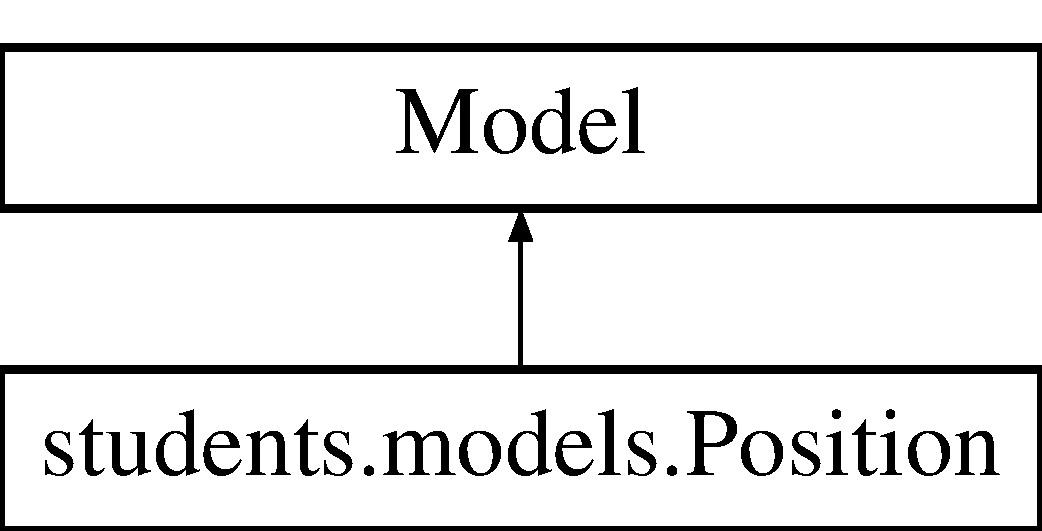
\includegraphics[height=2.000000cm]{classstudents_1_1models_1_1_position}
\end{center}
\end{figure}
\subsection*{Public Member Functions}
\begin{DoxyCompactItemize}
\item 
def \hyperlink{classstudents_1_1models_1_1_position_a9801bf25c27f58f0d7306f8df13b400e}{\-\_\-\-\_\-unicode\-\_\-\-\_\-}
\item 
def \hyperlink{classstudents_1_1models_1_1_position_ae6db8ec9d406188f652ec3d344f67f7b}{get\-\_\-jobtitle}
\end{DoxyCompactItemize}
\subsection*{Static Public Attributes}
\begin{DoxyCompactItemize}
\item 
tuple \hyperlink{classstudents_1_1models_1_1_position_ac2b78c8bf158e58d59783e6ec2a3507f}{start\-Date} = models.\-Char\-Field(max\-\_\-length=20)
\item 
tuple \hyperlink{classstudents_1_1models_1_1_position_ae2f7035f644cc07659733c538cc17672}{end\-Date} = models.\-Char\-Field(max\-\_\-length=20)
\item 
tuple \hyperlink{classstudents_1_1models_1_1_position_ac37b3ab263fab4dec8977add069b5bf6}{company} = models.\-Char\-Field(max\-\_\-length=100)
\item 
tuple \hyperlink{classstudents_1_1models_1_1_position_a20d8abf316914fea1d9f69d26c531759}{jobtitle} = models.\-Char\-Field(max\-\_\-length=100)
\item 
tuple \hyperlink{classstudents_1_1models_1_1_position_a5946dc44ba06da0bc7e92d7e2b3c3cab}{is\-Current} = models.\-Boolean\-Field(default=False)
\item 
tuple \hyperlink{classstudents_1_1models_1_1_position_ad2df3949444f644d538a93d7e829f9f7}{profile} = models.\-Foreign\-Key(\hyperlink{classstudents_1_1models_1_1_linked_in_profile}{Linked\-In\-Profile})
\end{DoxyCompactItemize}


\subsection{Detailed Description}
\begin{DoxyVerb}Model that represents a job position on LinkedIn.
\end{DoxyVerb}
 

\subsection{Member Function Documentation}
\hypertarget{classstudents_1_1models_1_1_position_a9801bf25c27f58f0d7306f8df13b400e}{\index{students\-::models\-::\-Position@{students\-::models\-::\-Position}!\-\_\-\-\_\-unicode\-\_\-\-\_\-@{\-\_\-\-\_\-unicode\-\_\-\-\_\-}}
\index{\-\_\-\-\_\-unicode\-\_\-\-\_\-@{\-\_\-\-\_\-unicode\-\_\-\-\_\-}!students::models::Position@{students\-::models\-::\-Position}}
\subsubsection[{\-\_\-\-\_\-unicode\-\_\-\-\_\-}]{\setlength{\rightskip}{0pt plus 5cm}def students.\-models.\-Position.\-\_\-\-\_\-unicode\-\_\-\-\_\- (
\begin{DoxyParamCaption}
\item[{}]{self}
\end{DoxyParamCaption}
)}}\label{classstudents_1_1models_1_1_position_a9801bf25c27f58f0d7306f8df13b400e}
\hypertarget{classstudents_1_1models_1_1_position_ae6db8ec9d406188f652ec3d344f67f7b}{\index{students\-::models\-::\-Position@{students\-::models\-::\-Position}!get\-\_\-jobtitle@{get\-\_\-jobtitle}}
\index{get\-\_\-jobtitle@{get\-\_\-jobtitle}!students::models::Position@{students\-::models\-::\-Position}}
\subsubsection[{get\-\_\-jobtitle}]{\setlength{\rightskip}{0pt plus 5cm}def students.\-models.\-Position.\-get\-\_\-jobtitle (
\begin{DoxyParamCaption}
\item[{}]{self}
\end{DoxyParamCaption}
)}}\label{classstudents_1_1models_1_1_position_ae6db8ec9d406188f652ec3d344f67f7b}


\subsection{Member Data Documentation}
\hypertarget{classstudents_1_1models_1_1_position_ac37b3ab263fab4dec8977add069b5bf6}{\index{students\-::models\-::\-Position@{students\-::models\-::\-Position}!company@{company}}
\index{company@{company}!students::models::Position@{students\-::models\-::\-Position}}
\subsubsection[{company}]{\setlength{\rightskip}{0pt plus 5cm}tuple students.\-models.\-Position.\-company = models.\-Char\-Field(max\-\_\-length=100)\hspace{0.3cm}{\ttfamily [static]}}}\label{classstudents_1_1models_1_1_position_ac37b3ab263fab4dec8977add069b5bf6}
\hypertarget{classstudents_1_1models_1_1_position_ae2f7035f644cc07659733c538cc17672}{\index{students\-::models\-::\-Position@{students\-::models\-::\-Position}!end\-Date@{end\-Date}}
\index{end\-Date@{end\-Date}!students::models::Position@{students\-::models\-::\-Position}}
\subsubsection[{end\-Date}]{\setlength{\rightskip}{0pt plus 5cm}tuple students.\-models.\-Position.\-end\-Date = models.\-Char\-Field(max\-\_\-length=20)\hspace{0.3cm}{\ttfamily [static]}}}\label{classstudents_1_1models_1_1_position_ae2f7035f644cc07659733c538cc17672}
\hypertarget{classstudents_1_1models_1_1_position_a5946dc44ba06da0bc7e92d7e2b3c3cab}{\index{students\-::models\-::\-Position@{students\-::models\-::\-Position}!is\-Current@{is\-Current}}
\index{is\-Current@{is\-Current}!students::models::Position@{students\-::models\-::\-Position}}
\subsubsection[{is\-Current}]{\setlength{\rightskip}{0pt plus 5cm}tuple students.\-models.\-Position.\-is\-Current = models.\-Boolean\-Field(default=False)\hspace{0.3cm}{\ttfamily [static]}}}\label{classstudents_1_1models_1_1_position_a5946dc44ba06da0bc7e92d7e2b3c3cab}
\hypertarget{classstudents_1_1models_1_1_position_a20d8abf316914fea1d9f69d26c531759}{\index{students\-::models\-::\-Position@{students\-::models\-::\-Position}!jobtitle@{jobtitle}}
\index{jobtitle@{jobtitle}!students::models::Position@{students\-::models\-::\-Position}}
\subsubsection[{jobtitle}]{\setlength{\rightskip}{0pt plus 5cm}tuple students.\-models.\-Position.\-jobtitle = models.\-Char\-Field(max\-\_\-length=100)\hspace{0.3cm}{\ttfamily [static]}}}\label{classstudents_1_1models_1_1_position_a20d8abf316914fea1d9f69d26c531759}
\hypertarget{classstudents_1_1models_1_1_position_ad2df3949444f644d538a93d7e829f9f7}{\index{students\-::models\-::\-Position@{students\-::models\-::\-Position}!profile@{profile}}
\index{profile@{profile}!students::models::Position@{students\-::models\-::\-Position}}
\subsubsection[{profile}]{\setlength{\rightskip}{0pt plus 5cm}tuple students.\-models.\-Position.\-profile = models.\-Foreign\-Key({\bf Linked\-In\-Profile})\hspace{0.3cm}{\ttfamily [static]}}}\label{classstudents_1_1models_1_1_position_ad2df3949444f644d538a93d7e829f9f7}
\hypertarget{classstudents_1_1models_1_1_position_ac2b78c8bf158e58d59783e6ec2a3507f}{\index{students\-::models\-::\-Position@{students\-::models\-::\-Position}!start\-Date@{start\-Date}}
\index{start\-Date@{start\-Date}!students::models::Position@{students\-::models\-::\-Position}}
\subsubsection[{start\-Date}]{\setlength{\rightskip}{0pt plus 5cm}tuple students.\-models.\-Position.\-start\-Date = models.\-Char\-Field(max\-\_\-length=20)\hspace{0.3cm}{\ttfamily [static]}}}\label{classstudents_1_1models_1_1_position_ac2b78c8bf158e58d59783e6ec2a3507f}


The documentation for this class was generated from the following file\-:\begin{DoxyCompactItemize}
\item 
leapkit/students/\hyperlink{models_8py}{models.\-py}\end{DoxyCompactItemize}

\hypertarget{classstudents_1_1linkedin__converter_1_1_position}{\section{students.\-linkedin\-\_\-converter.\-Position Class Reference}
\label{classstudents_1_1linkedin__converter_1_1_position}\index{students.\-linkedin\-\_\-converter.\-Position@{students.\-linkedin\-\_\-converter.\-Position}}
}
Inheritance diagram for students.\-linkedin\-\_\-converter.\-Position\-:\begin{figure}[H]
\begin{center}
\leavevmode
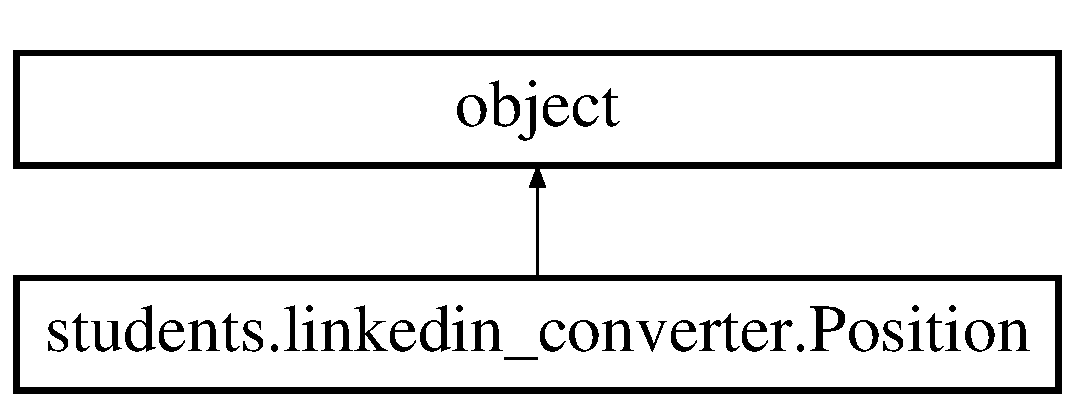
\includegraphics[height=2.000000cm]{classstudents_1_1linkedin__converter_1_1_position}
\end{center}
\end{figure}
\subsection*{Static Public Attributes}
\begin{DoxyCompactItemize}
\item 
string \hyperlink{classstudents_1_1linkedin__converter_1_1_position_ab8f28f8c86b50b641ffcdd18d3f7ada0}{end\-Date} = \char`\"{}\char`\"{}
\item 
string \hyperlink{classstudents_1_1linkedin__converter_1_1_position_ac6b8e26d676d6bf6c15c51012da90b85}{start\-Date} = \char`\"{}\char`\"{}
\item 
string \hyperlink{classstudents_1_1linkedin__converter_1_1_position_adac50b99cf25ff1739c0ef8e47790513}{is\-Current} = \char`\"{}\char`\"{}
\item 
string \hyperlink{classstudents_1_1linkedin__converter_1_1_position_abe1e57418151824f223a6df106bad11d}{pid} = \char`\"{}\char`\"{}
\item 
string \hyperlink{classstudents_1_1linkedin__converter_1_1_position_a4f0acf8538a488daedd9091f7f86dc8c}{company} = \char`\"{}\char`\"{}
\item 
string \hyperlink{classstudents_1_1linkedin__converter_1_1_position_a63ef787690c1859c3cb6ca8c18899c94}{title} = \char`\"{}\char`\"{}
\item 
string \hyperlink{classstudents_1_1linkedin__converter_1_1_position_a99344e54d4a5f380c7a224b440e3712e}{summary} = \char`\"{}\char`\"{}
\end{DoxyCompactItemize}


\subsection{Detailed Description}
\begin{DoxyVerb}A Position is used to hold the company positions and employment dration a person knows.\end{DoxyVerb}
\begin{DoxyVerb}Constructor that initiates all the basic position values\end{DoxyVerb}
 

\subsection{Member Data Documentation}
\hypertarget{classstudents_1_1linkedin__converter_1_1_position_a4f0acf8538a488daedd9091f7f86dc8c}{\index{students\-::linkedin\-\_\-converter\-::\-Position@{students\-::linkedin\-\_\-converter\-::\-Position}!company@{company}}
\index{company@{company}!students::linkedin_converter::Position@{students\-::linkedin\-\_\-converter\-::\-Position}}
\subsubsection[{company}]{\setlength{\rightskip}{0pt plus 5cm}string students.\-linkedin\-\_\-converter.\-Position.\-company = \char`\"{}\char`\"{}\hspace{0.3cm}{\ttfamily [static]}}}\label{classstudents_1_1linkedin__converter_1_1_position_a4f0acf8538a488daedd9091f7f86dc8c}
\hypertarget{classstudents_1_1linkedin__converter_1_1_position_ab8f28f8c86b50b641ffcdd18d3f7ada0}{\index{students\-::linkedin\-\_\-converter\-::\-Position@{students\-::linkedin\-\_\-converter\-::\-Position}!end\-Date@{end\-Date}}
\index{end\-Date@{end\-Date}!students::linkedin_converter::Position@{students\-::linkedin\-\_\-converter\-::\-Position}}
\subsubsection[{end\-Date}]{\setlength{\rightskip}{0pt plus 5cm}string students.\-linkedin\-\_\-converter.\-Position.\-end\-Date = \char`\"{}\char`\"{}\hspace{0.3cm}{\ttfamily [static]}}}\label{classstudents_1_1linkedin__converter_1_1_position_ab8f28f8c86b50b641ffcdd18d3f7ada0}
\hypertarget{classstudents_1_1linkedin__converter_1_1_position_adac50b99cf25ff1739c0ef8e47790513}{\index{students\-::linkedin\-\_\-converter\-::\-Position@{students\-::linkedin\-\_\-converter\-::\-Position}!is\-Current@{is\-Current}}
\index{is\-Current@{is\-Current}!students::linkedin_converter::Position@{students\-::linkedin\-\_\-converter\-::\-Position}}
\subsubsection[{is\-Current}]{\setlength{\rightskip}{0pt plus 5cm}string students.\-linkedin\-\_\-converter.\-Position.\-is\-Current = \char`\"{}\char`\"{}\hspace{0.3cm}{\ttfamily [static]}}}\label{classstudents_1_1linkedin__converter_1_1_position_adac50b99cf25ff1739c0ef8e47790513}
\hypertarget{classstudents_1_1linkedin__converter_1_1_position_abe1e57418151824f223a6df106bad11d}{\index{students\-::linkedin\-\_\-converter\-::\-Position@{students\-::linkedin\-\_\-converter\-::\-Position}!pid@{pid}}
\index{pid@{pid}!students::linkedin_converter::Position@{students\-::linkedin\-\_\-converter\-::\-Position}}
\subsubsection[{pid}]{\setlength{\rightskip}{0pt plus 5cm}string students.\-linkedin\-\_\-converter.\-Position.\-pid = \char`\"{}\char`\"{}\hspace{0.3cm}{\ttfamily [static]}}}\label{classstudents_1_1linkedin__converter_1_1_position_abe1e57418151824f223a6df106bad11d}
\hypertarget{classstudents_1_1linkedin__converter_1_1_position_ac6b8e26d676d6bf6c15c51012da90b85}{\index{students\-::linkedin\-\_\-converter\-::\-Position@{students\-::linkedin\-\_\-converter\-::\-Position}!start\-Date@{start\-Date}}
\index{start\-Date@{start\-Date}!students::linkedin_converter::Position@{students\-::linkedin\-\_\-converter\-::\-Position}}
\subsubsection[{start\-Date}]{\setlength{\rightskip}{0pt plus 5cm}string students.\-linkedin\-\_\-converter.\-Position.\-start\-Date = \char`\"{}\char`\"{}\hspace{0.3cm}{\ttfamily [static]}}}\label{classstudents_1_1linkedin__converter_1_1_position_ac6b8e26d676d6bf6c15c51012da90b85}
\hypertarget{classstudents_1_1linkedin__converter_1_1_position_a99344e54d4a5f380c7a224b440e3712e}{\index{students\-::linkedin\-\_\-converter\-::\-Position@{students\-::linkedin\-\_\-converter\-::\-Position}!summary@{summary}}
\index{summary@{summary}!students::linkedin_converter::Position@{students\-::linkedin\-\_\-converter\-::\-Position}}
\subsubsection[{summary}]{\setlength{\rightskip}{0pt plus 5cm}string students.\-linkedin\-\_\-converter.\-Position.\-summary = \char`\"{}\char`\"{}\hspace{0.3cm}{\ttfamily [static]}}}\label{classstudents_1_1linkedin__converter_1_1_position_a99344e54d4a5f380c7a224b440e3712e}
\hypertarget{classstudents_1_1linkedin__converter_1_1_position_a63ef787690c1859c3cb6ca8c18899c94}{\index{students\-::linkedin\-\_\-converter\-::\-Position@{students\-::linkedin\-\_\-converter\-::\-Position}!title@{title}}
\index{title@{title}!students::linkedin_converter::Position@{students\-::linkedin\-\_\-converter\-::\-Position}}
\subsubsection[{title}]{\setlength{\rightskip}{0pt plus 5cm}string students.\-linkedin\-\_\-converter.\-Position.\-title = \char`\"{}\char`\"{}\hspace{0.3cm}{\ttfamily [static]}}}\label{classstudents_1_1linkedin__converter_1_1_position_a63ef787690c1859c3cb6ca8c18899c94}


The documentation for this class was generated from the following file\-:\begin{DoxyCompactItemize}
\item 
leapkit/students/\hyperlink{linkedin__converter_8py}{linkedin\-\_\-converter.\-py}\end{DoxyCompactItemize}

\hypertarget{classstudents_1_1admin_1_1_position_admin}{\section{students.\-admin.\-Position\-Admin Class Reference}
\label{classstudents_1_1admin_1_1_position_admin}\index{students.\-admin.\-Position\-Admin@{students.\-admin.\-Position\-Admin}}
}
Inheritance diagram for students.\-admin.\-Position\-Admin\-:\begin{figure}[H]
\begin{center}
\leavevmode
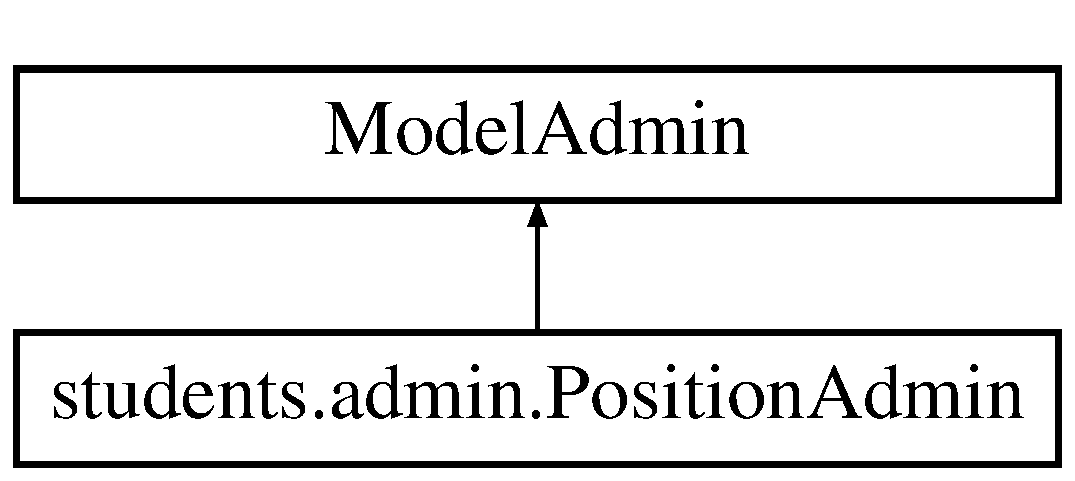
\includegraphics[height=2.000000cm]{classstudents_1_1admin_1_1_position_admin}
\end{center}
\end{figure}
\subsection*{Static Public Attributes}
\begin{DoxyCompactItemize}
\item 
list \hyperlink{classstudents_1_1admin_1_1_position_admin_ae4bf16213a76a16c62a36c5b68b6800b}{fieldsets}
\item 
tuple \hyperlink{classstudents_1_1admin_1_1_position_admin_a2b0a01f8594cfa3438e55d2d61bb3e05}{list\-\_\-display} = ('jobtitle', 'profile')
\item 
list \hyperlink{classstudents_1_1admin_1_1_position_admin_ae3055ae3ee6dd5e1b60b35b818f0ad1f}{search\-\_\-fields} = \mbox{[}'jobtitle', 'company', 'is\-Current', 'profile'\mbox{]}
\end{DoxyCompactItemize}


\subsection{Member Data Documentation}
\hypertarget{classstudents_1_1admin_1_1_position_admin_ae4bf16213a76a16c62a36c5b68b6800b}{\index{students\-::admin\-::\-Position\-Admin@{students\-::admin\-::\-Position\-Admin}!fieldsets@{fieldsets}}
\index{fieldsets@{fieldsets}!students::admin::PositionAdmin@{students\-::admin\-::\-Position\-Admin}}
\subsubsection[{fieldsets}]{\setlength{\rightskip}{0pt plus 5cm}list students.\-admin.\-Position\-Admin.\-fieldsets\hspace{0.3cm}{\ttfamily [static]}}}\label{classstudents_1_1admin_1_1_position_admin_ae4bf16213a76a16c62a36c5b68b6800b}
{\bfseries Initial value\-:}
\begin{DoxyCode}
1 = [(\textcolor{keywordtype}{None}, \{\textcolor{stringliteral}{'fields'} : [\textcolor{stringliteral}{'jobtitle'}, \textcolor{stringliteral}{'company'}, \textcolor{stringliteral}{'isCurrent'},
2         \textcolor{stringliteral}{'profile'}]\}),]
\end{DoxyCode}
\hypertarget{classstudents_1_1admin_1_1_position_admin_a2b0a01f8594cfa3438e55d2d61bb3e05}{\index{students\-::admin\-::\-Position\-Admin@{students\-::admin\-::\-Position\-Admin}!list\-\_\-display@{list\-\_\-display}}
\index{list\-\_\-display@{list\-\_\-display}!students::admin::PositionAdmin@{students\-::admin\-::\-Position\-Admin}}
\subsubsection[{list\-\_\-display}]{\setlength{\rightskip}{0pt plus 5cm}tuple students.\-admin.\-Position\-Admin.\-list\-\_\-display = ('jobtitle', 'profile')\hspace{0.3cm}{\ttfamily [static]}}}\label{classstudents_1_1admin_1_1_position_admin_a2b0a01f8594cfa3438e55d2d61bb3e05}
\hypertarget{classstudents_1_1admin_1_1_position_admin_ae3055ae3ee6dd5e1b60b35b818f0ad1f}{\index{students\-::admin\-::\-Position\-Admin@{students\-::admin\-::\-Position\-Admin}!search\-\_\-fields@{search\-\_\-fields}}
\index{search\-\_\-fields@{search\-\_\-fields}!students::admin::PositionAdmin@{students\-::admin\-::\-Position\-Admin}}
\subsubsection[{search\-\_\-fields}]{\setlength{\rightskip}{0pt plus 5cm}list students.\-admin.\-Position\-Admin.\-search\-\_\-fields = \mbox{[}'jobtitle', 'company', 'is\-Current', 'profile'\mbox{]}\hspace{0.3cm}{\ttfamily [static]}}}\label{classstudents_1_1admin_1_1_position_admin_ae3055ae3ee6dd5e1b60b35b818f0ad1f}


The documentation for this class was generated from the following file\-:\begin{DoxyCompactItemize}
\item 
leapkit/students/\hyperlink{admin_8py}{admin.\-py}\end{DoxyCompactItemize}

\hypertarget{classstudents_1_1views_1_1_send_mail_view}{\section{students.\-views.\-Send\-Mail\-View Class Reference}
\label{classstudents_1_1views_1_1_send_mail_view}\index{students.\-views.\-Send\-Mail\-View@{students.\-views.\-Send\-Mail\-View}}
}
Inheritance diagram for students.\-views.\-Send\-Mail\-View\-:\begin{figure}[H]
\begin{center}
\leavevmode
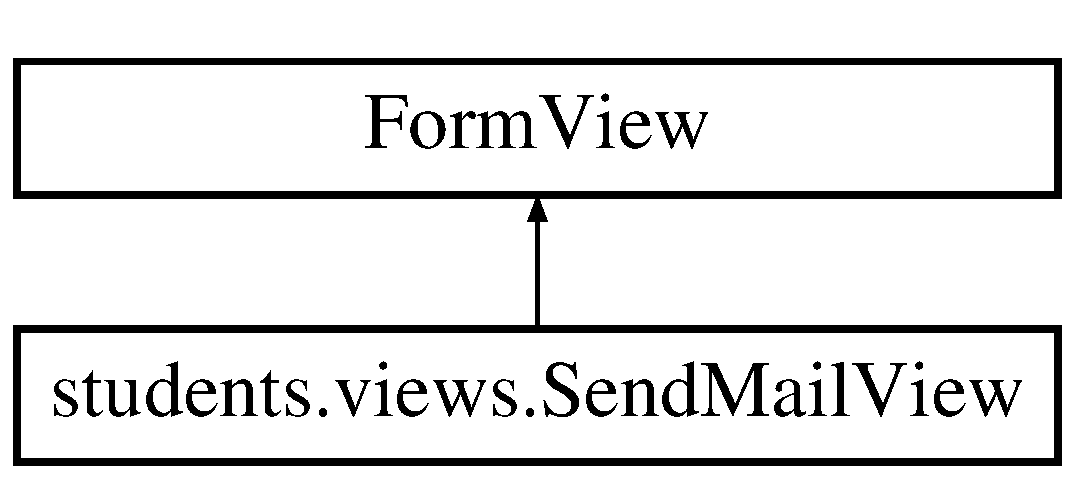
\includegraphics[height=2.000000cm]{classstudents_1_1views_1_1_send_mail_view}
\end{center}
\end{figure}
\subsection*{Public Member Functions}
\begin{DoxyCompactItemize}
\item 
def \hyperlink{classstudents_1_1views_1_1_send_mail_view_a41cb4edae96b73f4a14a62bbe3e02b3f}{get\-\_\-context\-\_\-data}
\item 
def \hyperlink{classstudents_1_1views_1_1_send_mail_view_a1a31847593c140f09be550af7e3db59a}{form\-\_\-valid}
\end{DoxyCompactItemize}
\subsection*{Static Public Attributes}
\begin{DoxyCompactItemize}
\item 
string \hyperlink{classstudents_1_1views_1_1_send_mail_view_a4441809c3bd7f631af7c5c4ccfed95e2}{template\-\_\-name} = \char`\"{}send\-\_\-email.\-html\char`\"{}
\item 
\hyperlink{classstudents_1_1views_1_1_send_mail_view_a66913d97023f49153b9f5aea5fa1fdc9}{form\-\_\-class} = Email\-Form
\end{DoxyCompactItemize}


\subsection{Member Function Documentation}
\hypertarget{classstudents_1_1views_1_1_send_mail_view_a1a31847593c140f09be550af7e3db59a}{\index{students\-::views\-::\-Send\-Mail\-View@{students\-::views\-::\-Send\-Mail\-View}!form\-\_\-valid@{form\-\_\-valid}}
\index{form\-\_\-valid@{form\-\_\-valid}!students::views::SendMailView@{students\-::views\-::\-Send\-Mail\-View}}
\subsubsection[{form\-\_\-valid}]{\setlength{\rightskip}{0pt plus 5cm}def students.\-views.\-Send\-Mail\-View.\-form\-\_\-valid (
\begin{DoxyParamCaption}
\item[{}]{self, }
\item[{}]{form}
\end{DoxyParamCaption}
)}}\label{classstudents_1_1views_1_1_send_mail_view_a1a31847593c140f09be550af7e3db59a}
\hypertarget{classstudents_1_1views_1_1_send_mail_view_a41cb4edae96b73f4a14a62bbe3e02b3f}{\index{students\-::views\-::\-Send\-Mail\-View@{students\-::views\-::\-Send\-Mail\-View}!get\-\_\-context\-\_\-data@{get\-\_\-context\-\_\-data}}
\index{get\-\_\-context\-\_\-data@{get\-\_\-context\-\_\-data}!students::views::SendMailView@{students\-::views\-::\-Send\-Mail\-View}}
\subsubsection[{get\-\_\-context\-\_\-data}]{\setlength{\rightskip}{0pt plus 5cm}def students.\-views.\-Send\-Mail\-View.\-get\-\_\-context\-\_\-data (
\begin{DoxyParamCaption}
\item[{}]{self, }
\item[{}]{kwargs}
\end{DoxyParamCaption}
)}}\label{classstudents_1_1views_1_1_send_mail_view_a41cb4edae96b73f4a14a62bbe3e02b3f}


\subsection{Member Data Documentation}
\hypertarget{classstudents_1_1views_1_1_send_mail_view_a66913d97023f49153b9f5aea5fa1fdc9}{\index{students\-::views\-::\-Send\-Mail\-View@{students\-::views\-::\-Send\-Mail\-View}!form\-\_\-class@{form\-\_\-class}}
\index{form\-\_\-class@{form\-\_\-class}!students::views::SendMailView@{students\-::views\-::\-Send\-Mail\-View}}
\subsubsection[{form\-\_\-class}]{\setlength{\rightskip}{0pt plus 5cm}students.\-views.\-Send\-Mail\-View.\-form\-\_\-class = Email\-Form\hspace{0.3cm}{\ttfamily [static]}}}\label{classstudents_1_1views_1_1_send_mail_view_a66913d97023f49153b9f5aea5fa1fdc9}
\hypertarget{classstudents_1_1views_1_1_send_mail_view_a4441809c3bd7f631af7c5c4ccfed95e2}{\index{students\-::views\-::\-Send\-Mail\-View@{students\-::views\-::\-Send\-Mail\-View}!template\-\_\-name@{template\-\_\-name}}
\index{template\-\_\-name@{template\-\_\-name}!students::views::SendMailView@{students\-::views\-::\-Send\-Mail\-View}}
\subsubsection[{template\-\_\-name}]{\setlength{\rightskip}{0pt plus 5cm}string students.\-views.\-Send\-Mail\-View.\-template\-\_\-name = \char`\"{}send\-\_\-email.\-html\char`\"{}\hspace{0.3cm}{\ttfamily [static]}}}\label{classstudents_1_1views_1_1_send_mail_view_a4441809c3bd7f631af7c5c4ccfed95e2}


The documentation for this class was generated from the following file\-:\begin{DoxyCompactItemize}
\item 
leapkit/students/\hyperlink{views_8py}{views.\-py}\end{DoxyCompactItemize}

\hypertarget{classstudents_1_1models_1_1_skill}{\section{students.\-models.\-Skill Class Reference}
\label{classstudents_1_1models_1_1_skill}\index{students.\-models.\-Skill@{students.\-models.\-Skill}}
}
Inheritance diagram for students.\-models.\-Skill\-:\begin{figure}[H]
\begin{center}
\leavevmode
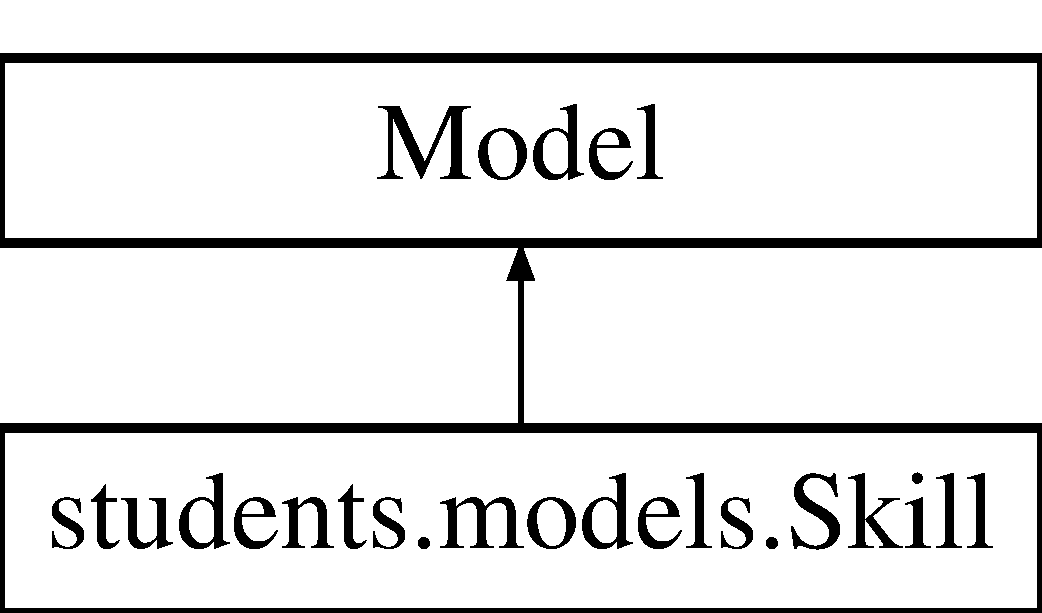
\includegraphics[height=2.000000cm]{classstudents_1_1models_1_1_skill}
\end{center}
\end{figure}
\subsection*{Public Member Functions}
\begin{DoxyCompactItemize}
\item 
def \hyperlink{classstudents_1_1models_1_1_skill_aef95ddd6ca24a649025dca066439af78}{\-\_\-\-\_\-unicode\-\_\-\-\_\-}
\item 
def \hyperlink{classstudents_1_1models_1_1_skill_a44f6a7c6975253c8f617f36c4400f19c}{get\-\_\-skill}
\end{DoxyCompactItemize}
\subsection*{Static Public Attributes}
\begin{DoxyCompactItemize}
\item 
tuple \hyperlink{classstudents_1_1models_1_1_skill_a5c22b1127793cd1ea56874c792f83c68}{name} = models.\-Char\-Field(max\-\_\-length = 81)
\item 
tuple \hyperlink{classstudents_1_1models_1_1_skill_aeb30b2427a9875143ebd154fd1a9503e}{profile} = models.\-Foreign\-Key(\hyperlink{classstudents_1_1models_1_1_linked_in_profile}{Linked\-In\-Profile})
\end{DoxyCompactItemize}


\subsection{Detailed Description}
\begin{DoxyVerb}Model that represents a skill on LinkedIn.
\end{DoxyVerb}
 

\subsection{Member Function Documentation}
\hypertarget{classstudents_1_1models_1_1_skill_aef95ddd6ca24a649025dca066439af78}{\index{students\-::models\-::\-Skill@{students\-::models\-::\-Skill}!\-\_\-\-\_\-unicode\-\_\-\-\_\-@{\-\_\-\-\_\-unicode\-\_\-\-\_\-}}
\index{\-\_\-\-\_\-unicode\-\_\-\-\_\-@{\-\_\-\-\_\-unicode\-\_\-\-\_\-}!students::models::Skill@{students\-::models\-::\-Skill}}
\subsubsection[{\-\_\-\-\_\-unicode\-\_\-\-\_\-}]{\setlength{\rightskip}{0pt plus 5cm}def students.\-models.\-Skill.\-\_\-\-\_\-unicode\-\_\-\-\_\- (
\begin{DoxyParamCaption}
\item[{}]{self}
\end{DoxyParamCaption}
)}}\label{classstudents_1_1models_1_1_skill_aef95ddd6ca24a649025dca066439af78}
\hypertarget{classstudents_1_1models_1_1_skill_a44f6a7c6975253c8f617f36c4400f19c}{\index{students\-::models\-::\-Skill@{students\-::models\-::\-Skill}!get\-\_\-skill@{get\-\_\-skill}}
\index{get\-\_\-skill@{get\-\_\-skill}!students::models::Skill@{students\-::models\-::\-Skill}}
\subsubsection[{get\-\_\-skill}]{\setlength{\rightskip}{0pt plus 5cm}def students.\-models.\-Skill.\-get\-\_\-skill (
\begin{DoxyParamCaption}
\item[{}]{self}
\end{DoxyParamCaption}
)}}\label{classstudents_1_1models_1_1_skill_a44f6a7c6975253c8f617f36c4400f19c}


\subsection{Member Data Documentation}
\hypertarget{classstudents_1_1models_1_1_skill_a5c22b1127793cd1ea56874c792f83c68}{\index{students\-::models\-::\-Skill@{students\-::models\-::\-Skill}!name@{name}}
\index{name@{name}!students::models::Skill@{students\-::models\-::\-Skill}}
\subsubsection[{name}]{\setlength{\rightskip}{0pt plus 5cm}tuple students.\-models.\-Skill.\-name = models.\-Char\-Field(max\-\_\-length = 81)\hspace{0.3cm}{\ttfamily [static]}}}\label{classstudents_1_1models_1_1_skill_a5c22b1127793cd1ea56874c792f83c68}
\hypertarget{classstudents_1_1models_1_1_skill_aeb30b2427a9875143ebd154fd1a9503e}{\index{students\-::models\-::\-Skill@{students\-::models\-::\-Skill}!profile@{profile}}
\index{profile@{profile}!students::models::Skill@{students\-::models\-::\-Skill}}
\subsubsection[{profile}]{\setlength{\rightskip}{0pt plus 5cm}tuple students.\-models.\-Skill.\-profile = models.\-Foreign\-Key({\bf Linked\-In\-Profile})\hspace{0.3cm}{\ttfamily [static]}}}\label{classstudents_1_1models_1_1_skill_aeb30b2427a9875143ebd154fd1a9503e}


The documentation for this class was generated from the following file\-:\begin{DoxyCompactItemize}
\item 
leapkit/students/\hyperlink{models_8py}{models.\-py}\end{DoxyCompactItemize}

\hypertarget{classstudents_1_1linkedin__converter_1_1_skill}{\section{students.\-linkedin\-\_\-converter.\-Skill Class Reference}
\label{classstudents_1_1linkedin__converter_1_1_skill}\index{students.\-linkedin\-\_\-converter.\-Skill@{students.\-linkedin\-\_\-converter.\-Skill}}
}
Inheritance diagram for students.\-linkedin\-\_\-converter.\-Skill\-:\begin{figure}[H]
\begin{center}
\leavevmode
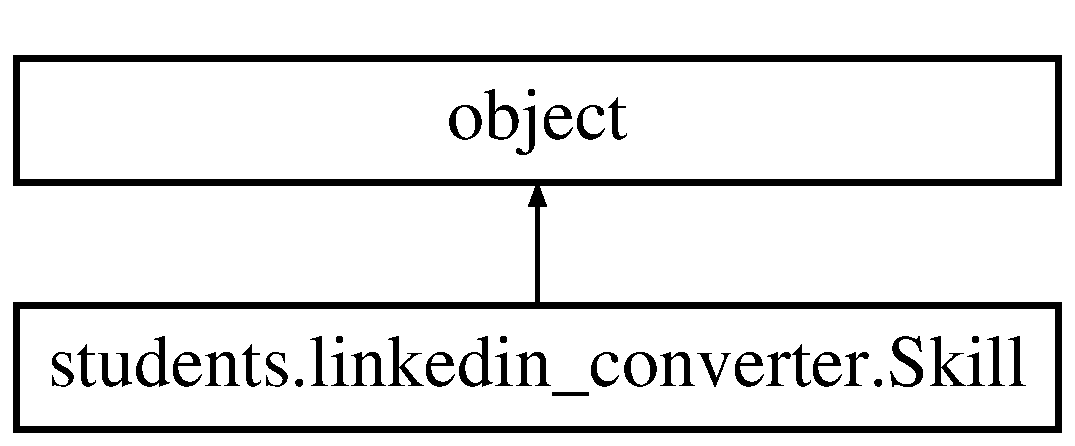
\includegraphics[height=2.000000cm]{classstudents_1_1linkedin__converter_1_1_skill}
\end{center}
\end{figure}
\subsection*{Static Public Attributes}
\begin{DoxyCompactItemize}
\item 
string \hyperlink{classstudents_1_1linkedin__converter_1_1_skill_a833fda242e2aa99c0b3d146fd02edfda}{sid} = \char`\"{}\char`\"{}
\item 
string \hyperlink{classstudents_1_1linkedin__converter_1_1_skill_a2d5ed72765fe5fb834aa89ece121e53e}{name} = \char`\"{}\char`\"{}
\end{DoxyCompactItemize}


\subsection{Detailed Description}
\begin{DoxyVerb}Skill is used to hold what skills a person has.\end{DoxyVerb}
\begin{DoxyVerb}Constructor that initiates all the basic skill values\end{DoxyVerb}
 

\subsection{Member Data Documentation}
\hypertarget{classstudents_1_1linkedin__converter_1_1_skill_a2d5ed72765fe5fb834aa89ece121e53e}{\index{students\-::linkedin\-\_\-converter\-::\-Skill@{students\-::linkedin\-\_\-converter\-::\-Skill}!name@{name}}
\index{name@{name}!students::linkedin_converter::Skill@{students\-::linkedin\-\_\-converter\-::\-Skill}}
\subsubsection[{name}]{\setlength{\rightskip}{0pt plus 5cm}string students.\-linkedin\-\_\-converter.\-Skill.\-name = \char`\"{}\char`\"{}\hspace{0.3cm}{\ttfamily [static]}}}\label{classstudents_1_1linkedin__converter_1_1_skill_a2d5ed72765fe5fb834aa89ece121e53e}
\hypertarget{classstudents_1_1linkedin__converter_1_1_skill_a833fda242e2aa99c0b3d146fd02edfda}{\index{students\-::linkedin\-\_\-converter\-::\-Skill@{students\-::linkedin\-\_\-converter\-::\-Skill}!sid@{sid}}
\index{sid@{sid}!students::linkedin_converter::Skill@{students\-::linkedin\-\_\-converter\-::\-Skill}}
\subsubsection[{sid}]{\setlength{\rightskip}{0pt plus 5cm}string students.\-linkedin\-\_\-converter.\-Skill.\-sid = \char`\"{}\char`\"{}\hspace{0.3cm}{\ttfamily [static]}}}\label{classstudents_1_1linkedin__converter_1_1_skill_a833fda242e2aa99c0b3d146fd02edfda}


The documentation for this class was generated from the following file\-:\begin{DoxyCompactItemize}
\item 
leapkit/students/\hyperlink{linkedin__converter_8py}{linkedin\-\_\-converter.\-py}\end{DoxyCompactItemize}

\hypertarget{classstudents_1_1admin_1_1_skill_admin}{\section{students.\-admin.\-Skill\-Admin Class Reference}
\label{classstudents_1_1admin_1_1_skill_admin}\index{students.\-admin.\-Skill\-Admin@{students.\-admin.\-Skill\-Admin}}
}
Inheritance diagram for students.\-admin.\-Skill\-Admin\-:\begin{figure}[H]
\begin{center}
\leavevmode
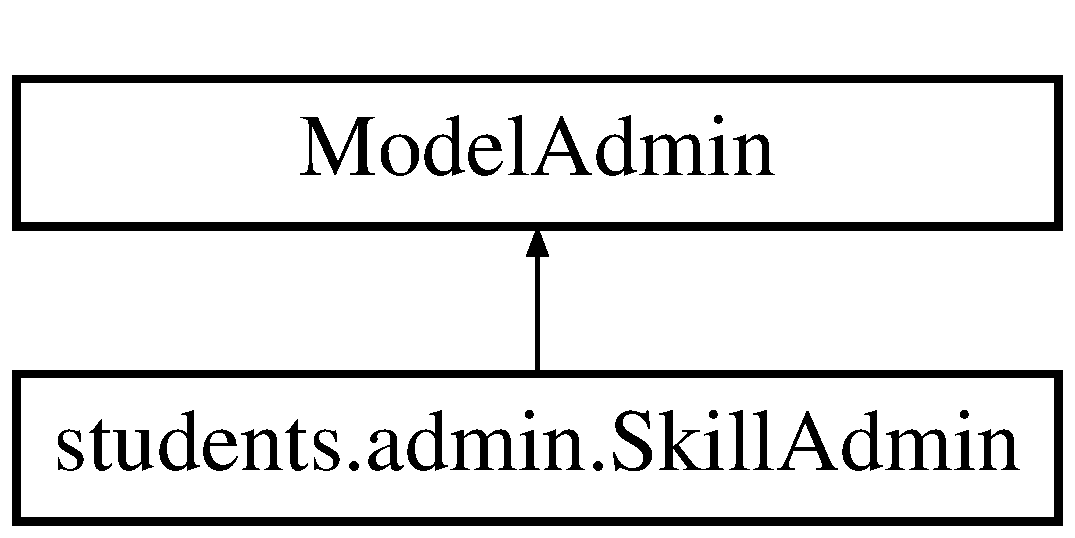
\includegraphics[height=2.000000cm]{classstudents_1_1admin_1_1_skill_admin}
\end{center}
\end{figure}
\subsection*{Static Public Attributes}
\begin{DoxyCompactItemize}
\item 
list \hyperlink{classstudents_1_1admin_1_1_skill_admin_a454e45e7078bd30e268d1e0c89a38575}{fieldsets} = \mbox{[}(None, \{'fields' \-: \mbox{[}'name', 'profile'\mbox{]}\}),\mbox{]}
\item 
tuple \hyperlink{classstudents_1_1admin_1_1_skill_admin_a91d65295b3213f8a1eec76ae8b9f43f7}{list\-\_\-display} = ('name', 'profile')
\item 
list \hyperlink{classstudents_1_1admin_1_1_skill_admin_a4ed1cf2d0e90b6f04b2cd387906b1952}{search\-\_\-fields} = \mbox{[}'name','profile'\mbox{]}
\end{DoxyCompactItemize}


\subsection{Member Data Documentation}
\hypertarget{classstudents_1_1admin_1_1_skill_admin_a454e45e7078bd30e268d1e0c89a38575}{\index{students\-::admin\-::\-Skill\-Admin@{students\-::admin\-::\-Skill\-Admin}!fieldsets@{fieldsets}}
\index{fieldsets@{fieldsets}!students::admin::SkillAdmin@{students\-::admin\-::\-Skill\-Admin}}
\subsubsection[{fieldsets}]{\setlength{\rightskip}{0pt plus 5cm}list students.\-admin.\-Skill\-Admin.\-fieldsets = \mbox{[}(None, \{'fields' \-: \mbox{[}'name', 'profile'\mbox{]}\}),\mbox{]}\hspace{0.3cm}{\ttfamily [static]}}}\label{classstudents_1_1admin_1_1_skill_admin_a454e45e7078bd30e268d1e0c89a38575}
\hypertarget{classstudents_1_1admin_1_1_skill_admin_a91d65295b3213f8a1eec76ae8b9f43f7}{\index{students\-::admin\-::\-Skill\-Admin@{students\-::admin\-::\-Skill\-Admin}!list\-\_\-display@{list\-\_\-display}}
\index{list\-\_\-display@{list\-\_\-display}!students::admin::SkillAdmin@{students\-::admin\-::\-Skill\-Admin}}
\subsubsection[{list\-\_\-display}]{\setlength{\rightskip}{0pt plus 5cm}tuple students.\-admin.\-Skill\-Admin.\-list\-\_\-display = ('name', 'profile')\hspace{0.3cm}{\ttfamily [static]}}}\label{classstudents_1_1admin_1_1_skill_admin_a91d65295b3213f8a1eec76ae8b9f43f7}
\hypertarget{classstudents_1_1admin_1_1_skill_admin_a4ed1cf2d0e90b6f04b2cd387906b1952}{\index{students\-::admin\-::\-Skill\-Admin@{students\-::admin\-::\-Skill\-Admin}!search\-\_\-fields@{search\-\_\-fields}}
\index{search\-\_\-fields@{search\-\_\-fields}!students::admin::SkillAdmin@{students\-::admin\-::\-Skill\-Admin}}
\subsubsection[{search\-\_\-fields}]{\setlength{\rightskip}{0pt plus 5cm}list students.\-admin.\-Skill\-Admin.\-search\-\_\-fields = \mbox{[}'name','profile'\mbox{]}\hspace{0.3cm}{\ttfamily [static]}}}\label{classstudents_1_1admin_1_1_skill_admin_a4ed1cf2d0e90b6f04b2cd387906b1952}


The documentation for this class was generated from the following file\-:\begin{DoxyCompactItemize}
\item 
leapkit/students/\hyperlink{admin_8py}{admin.\-py}\end{DoxyCompactItemize}

\hypertarget{classstudents_1_1models_1_1_student}{\section{students.\-models.\-Student Class Reference}
\label{classstudents_1_1models_1_1_student}\index{students.\-models.\-Student@{students.\-models.\-Student}}
}
Inheritance diagram for students.\-models.\-Student\-:\begin{figure}[H]
\begin{center}
\leavevmode
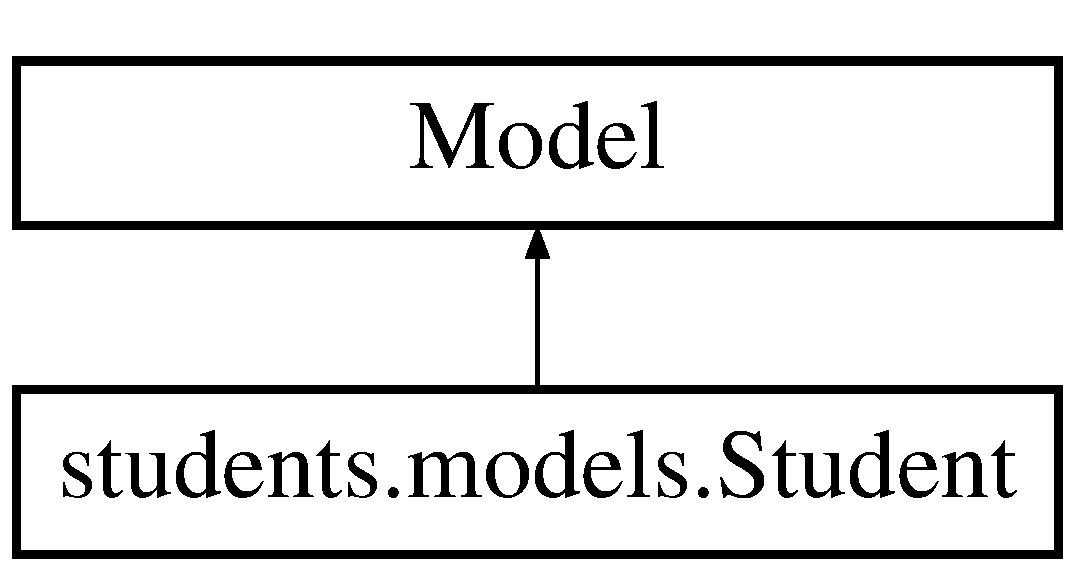
\includegraphics[height=2.000000cm]{classstudents_1_1models_1_1_student}
\end{center}
\end{figure}
\subsection*{Public Member Functions}
\begin{DoxyCompactItemize}
\item 
def \hyperlink{classstudents_1_1models_1_1_student_a9d4928c942577b10f9d2ba8a99c21fee}{\-\_\-\-\_\-unicode\-\_\-\-\_\-}
\item 
def \hyperlink{classstudents_1_1models_1_1_student_acad8d7a62069a546d1e3a5f96a7fd971}{get\-\_\-full\-\_\-name}
\item 
def \hyperlink{classstudents_1_1models_1_1_student_adb4699e44c6376397ce441fc8694840e}{get\-\_\-short\-\_\-name}
\item 
def \hyperlink{classstudents_1_1models_1_1_student_a435641b741a8020d3abb4a356867fbb0}{get\-\_\-absolute\-\_\-update\-\_\-url}
\item 
def \hyperlink{classstudents_1_1models_1_1_student_ae9125f2c920f8b915e714d58bade580d}{get\-\_\-absolute\-\_\-url}
\item 
def \hyperlink{classstudents_1_1models_1_1_student_a7d9cc5b28b8b29fafd91020c3ab7bb96}{save}
\item 
def \hyperlink{classstudents_1_1models_1_1_student_adb3818c664b585eecc100caf80d3f529}{send\-\_\-activation\-\_\-email}
\item 
def \hyperlink{classstudents_1_1models_1_1_student_ab1ff0197cbfbdbfac52b54a9bc51e592}{unique\-\_\-slugify}
\end{DoxyCompactItemize}
\subsection*{Public Attributes}
\begin{DoxyCompactItemize}
\item 
\hyperlink{classstudents_1_1models_1_1_student_a6f81eac38fb0a6074eb663b3cab8055e}{image}
\end{DoxyCompactItemize}
\subsection*{Static Public Attributes}
\begin{DoxyCompactItemize}
\item 
string \hyperlink{classstudents_1_1models_1_1_student_ab3c1ac4f87bcca2bb3e6bcf319aef7b7}{M\-A\-L\-E} = \char`\"{}M\char`\"{}
\item 
string \hyperlink{classstudents_1_1models_1_1_student_a8de6077045683c830b41fcd0a41c4a8a}{F\-E\-M\-A\-L\-E} = \char`\"{}F\char`\"{}
\item 
dictionary \hyperlink{classstudents_1_1models_1_1_student_a2a85491d6d3ae6efdbdd58da14ec01fa}{S\-E\-X}
\item 
tuple \hyperlink{classstudents_1_1models_1_1_student_a7c56f44c930c1bcdd80f8f8860af5bee}{user} = models.\-One\-To\-One\-Field(User, unique=True, blank=True)
\item 
tuple \hyperlink{classstudents_1_1models_1_1_student_a37eca324de73539147a0083dfdf735ac}{image}
\item 
tuple \hyperlink{classstudents_1_1models_1_1_student_a9254eb630a5d3de52a566b11c8ab6f1b}{times\-\_\-logged\-\_\-in} = models.\-Integer\-Field(default=1)
\item 
tuple \hyperlink{classstudents_1_1models_1_1_student_a3fa9119af0d1c42d0beafad3d90b8153}{first\-\_\-name} = models.\-Char\-Field(max\-\_\-length=100)
\item 
tuple \hyperlink{classstudents_1_1models_1_1_student_a851aa51a430028eb921054a10e79a599}{last\-\_\-name} = models.\-Char\-Field(max\-\_\-length=100)
\item 
tuple \hyperlink{classstudents_1_1models_1_1_student_af7f5dc2a714b4a00ceac864f96a5126c}{date\-\_\-of\-\_\-birth}
\item 
tuple \hyperlink{classstudents_1_1models_1_1_student_ae8f0e56e008cc61770d2f0f5b5ca6182}{gender}
\item 
tuple \hyperlink{classstudents_1_1models_1_1_student_a904985debef148d1871397fbdd756c91}{date\-\_\-joined} = models.\-Date\-Time\-Field(auto\-\_\-now=True)
\item 
tuple \hyperlink{classstudents_1_1models_1_1_student_aa7e41320bd36856721a6401b23a7eb3e}{modified} = models.\-Date\-Time\-Field(auto\-\_\-now\-\_\-add=True)
\item 
tuple \hyperlink{classstudents_1_1models_1_1_student_ad676823e45f40a8f3bd16e2cb2a96946}{slug} = models.\-Slug\-Field(max\-\_\-length=255, unique=True, blank=True)
\item 
string \hyperlink{classstudents_1_1models_1_1_student_a44c22f24f6430caa8c30a11cc2eda2f9}{B\-A\-C\-H\-E\-L\-O\-R} = \char`\"{}B\-S\-C\char`\"{}
\item 
string \hyperlink{classstudents_1_1models_1_1_student_a96eaf2a1b27d151cc511133ded581dc4}{M\-A\-S\-T\-E\-R} = \char`\"{}M\-S\-C\char`\"{}
\item 
dictionary \hyperlink{classstudents_1_1models_1_1_student_a8f86f0fb0935aa98bf4e4c662c144943}{E\-D\-U\-C\-T\-A\-T\-I\-O\-N\-\_\-\-L\-E\-V\-E\-L}
\item 
tuple \hyperlink{classstudents_1_1models_1_1_student_a43909b3b49d600bfb53f10286a838fe0}{education\-\_\-level}
\item 
tuple \hyperlink{classstudents_1_1models_1_1_student_a03e45fddb9a4c1cd701ecf71ce750b55}{country}
\item 
tuple \hyperlink{classstudents_1_1models_1_1_student_a4c97e38c90574a31ad7a4604ee731128}{region}
\item 
tuple \hyperlink{classstudents_1_1models_1_1_student_a276c47ab433d4e1f7e4aff01036bd9cf}{zip\-\_\-code}
\item 
tuple \hyperlink{classstudents_1_1models_1_1_student_ac237b28a8bc0d6f538fcfcb64f1bbede}{city}
\item 
tuple \hyperlink{classstudents_1_1models_1_1_student_a389b723936a0a1ca5f8327563c1a7187}{street}
\item 
tuple \hyperlink{classstudents_1_1models_1_1_student_a41718377a531d1677d8196ac292ccb43}{institution}
\item 
tuple \hyperlink{classstudents_1_1models_1_1_student_ab9b3060609019e2bc54a43d2e09c0cbd}{department}
\item 
tuple \hyperlink{classstudents_1_1models_1_1_student_a08fe0c93f50c6a1699ff506a76ef3172}{courses}
\item 
tuple \hyperlink{classstudents_1_1models_1_1_student_af95758393c5324d289f2b24441222b32}{line\-\_\-of\-\_\-study}
\item 
tuple \hyperlink{classstudents_1_1models_1_1_student_a56967491948903227152a9fa074c9546}{description}
\item 
tuple \hyperlink{classstudents_1_1models_1_1_student_ad1da7d6dcdd52dcef337cf689b329e19}{cv}
\end{DoxyCompactItemize}


\subsection{Member Function Documentation}
\hypertarget{classstudents_1_1models_1_1_student_a9d4928c942577b10f9d2ba8a99c21fee}{\index{students\-::models\-::\-Student@{students\-::models\-::\-Student}!\-\_\-\-\_\-unicode\-\_\-\-\_\-@{\-\_\-\-\_\-unicode\-\_\-\-\_\-}}
\index{\-\_\-\-\_\-unicode\-\_\-\-\_\-@{\-\_\-\-\_\-unicode\-\_\-\-\_\-}!students::models::Student@{students\-::models\-::\-Student}}
\subsubsection[{\-\_\-\-\_\-unicode\-\_\-\-\_\-}]{\setlength{\rightskip}{0pt plus 5cm}def students.\-models.\-Student.\-\_\-\-\_\-unicode\-\_\-\-\_\- (
\begin{DoxyParamCaption}
\item[{}]{self}
\end{DoxyParamCaption}
)}}\label{classstudents_1_1models_1_1_student_a9d4928c942577b10f9d2ba8a99c21fee}
\hypertarget{classstudents_1_1models_1_1_student_a435641b741a8020d3abb4a356867fbb0}{\index{students\-::models\-::\-Student@{students\-::models\-::\-Student}!get\-\_\-absolute\-\_\-update\-\_\-url@{get\-\_\-absolute\-\_\-update\-\_\-url}}
\index{get\-\_\-absolute\-\_\-update\-\_\-url@{get\-\_\-absolute\-\_\-update\-\_\-url}!students::models::Student@{students\-::models\-::\-Student}}
\subsubsection[{get\-\_\-absolute\-\_\-update\-\_\-url}]{\setlength{\rightskip}{0pt plus 5cm}def students.\-models.\-Student.\-get\-\_\-absolute\-\_\-update\-\_\-url (
\begin{DoxyParamCaption}
\item[{}]{self}
\end{DoxyParamCaption}
)}}\label{classstudents_1_1models_1_1_student_a435641b741a8020d3abb4a356867fbb0}
\hypertarget{classstudents_1_1models_1_1_student_ae9125f2c920f8b915e714d58bade580d}{\index{students\-::models\-::\-Student@{students\-::models\-::\-Student}!get\-\_\-absolute\-\_\-url@{get\-\_\-absolute\-\_\-url}}
\index{get\-\_\-absolute\-\_\-url@{get\-\_\-absolute\-\_\-url}!students::models::Student@{students\-::models\-::\-Student}}
\subsubsection[{get\-\_\-absolute\-\_\-url}]{\setlength{\rightskip}{0pt plus 5cm}def students.\-models.\-Student.\-get\-\_\-absolute\-\_\-url (
\begin{DoxyParamCaption}
\item[{}]{self}
\end{DoxyParamCaption}
)}}\label{classstudents_1_1models_1_1_student_ae9125f2c920f8b915e714d58bade580d}
\hypertarget{classstudents_1_1models_1_1_student_acad8d7a62069a546d1e3a5f96a7fd971}{\index{students\-::models\-::\-Student@{students\-::models\-::\-Student}!get\-\_\-full\-\_\-name@{get\-\_\-full\-\_\-name}}
\index{get\-\_\-full\-\_\-name@{get\-\_\-full\-\_\-name}!students::models::Student@{students\-::models\-::\-Student}}
\subsubsection[{get\-\_\-full\-\_\-name}]{\setlength{\rightskip}{0pt plus 5cm}def students.\-models.\-Student.\-get\-\_\-full\-\_\-name (
\begin{DoxyParamCaption}
\item[{}]{self}
\end{DoxyParamCaption}
)}}\label{classstudents_1_1models_1_1_student_acad8d7a62069a546d1e3a5f96a7fd971}
\begin{DoxyVerb}:return: First name + last name, with a space in between
\end{DoxyVerb}
 \hypertarget{classstudents_1_1models_1_1_student_adb4699e44c6376397ce441fc8694840e}{\index{students\-::models\-::\-Student@{students\-::models\-::\-Student}!get\-\_\-short\-\_\-name@{get\-\_\-short\-\_\-name}}
\index{get\-\_\-short\-\_\-name@{get\-\_\-short\-\_\-name}!students::models::Student@{students\-::models\-::\-Student}}
\subsubsection[{get\-\_\-short\-\_\-name}]{\setlength{\rightskip}{0pt plus 5cm}def students.\-models.\-Student.\-get\-\_\-short\-\_\-name (
\begin{DoxyParamCaption}
\item[{}]{self}
\end{DoxyParamCaption}
)}}\label{classstudents_1_1models_1_1_student_adb4699e44c6376397ce441fc8694840e}
\begin{DoxyVerb}:return: email
\end{DoxyVerb}
 \hypertarget{classstudents_1_1models_1_1_student_a7d9cc5b28b8b29fafd91020c3ab7bb96}{\index{students\-::models\-::\-Student@{students\-::models\-::\-Student}!save@{save}}
\index{save@{save}!students::models::Student@{students\-::models\-::\-Student}}
\subsubsection[{save}]{\setlength{\rightskip}{0pt plus 5cm}def students.\-models.\-Student.\-save (
\begin{DoxyParamCaption}
\item[{}]{self, }
\item[{}]{args, }
\item[{}]{kwargs}
\end{DoxyParamCaption}
)}}\label{classstudents_1_1models_1_1_student_a7d9cc5b28b8b29fafd91020c3ab7bb96}
\hypertarget{classstudents_1_1models_1_1_student_adb3818c664b585eecc100caf80d3f529}{\index{students\-::models\-::\-Student@{students\-::models\-::\-Student}!send\-\_\-activation\-\_\-email@{send\-\_\-activation\-\_\-email}}
\index{send\-\_\-activation\-\_\-email@{send\-\_\-activation\-\_\-email}!students::models::Student@{students\-::models\-::\-Student}}
\subsubsection[{send\-\_\-activation\-\_\-email}]{\setlength{\rightskip}{0pt plus 5cm}def students.\-models.\-Student.\-send\-\_\-activation\-\_\-email (
\begin{DoxyParamCaption}
\item[{}]{self}
\end{DoxyParamCaption}
)}}\label{classstudents_1_1models_1_1_student_adb3818c664b585eecc100caf80d3f529}
\hypertarget{classstudents_1_1models_1_1_student_ab1ff0197cbfbdbfac52b54a9bc51e592}{\index{students\-::models\-::\-Student@{students\-::models\-::\-Student}!unique\-\_\-slugify@{unique\-\_\-slugify}}
\index{unique\-\_\-slugify@{unique\-\_\-slugify}!students::models::Student@{students\-::models\-::\-Student}}
\subsubsection[{unique\-\_\-slugify}]{\setlength{\rightskip}{0pt plus 5cm}def students.\-models.\-Student.\-unique\-\_\-slugify (
\begin{DoxyParamCaption}
\item[{}]{instance, }
\item[{}]{value, }
\item[{}]{slug\-\_\-field\-\_\-name = {\ttfamily '{\bf slug}'}, }
\item[{}]{queryset = {\ttfamily None}, }
\item[{}]{slug\-\_\-separator = {\ttfamily '-\/'}}
\end{DoxyParamCaption}
)}}\label{classstudents_1_1models_1_1_student_ab1ff0197cbfbdbfac52b54a9bc51e592}
\begin{DoxyVerb}Calculates and stores a unique slug of ``value`` for an instance.

``slug_field_name`` should be a string matching the name of the field to
store the slug in (and the field to check against for uniqueness).

``queryset`` usually doesn't need to be explicitly provided - it'll default
to using the ``.all()`` queryset from the model's default manager.
\end{DoxyVerb}
 

\subsection{Member Data Documentation}
\hypertarget{classstudents_1_1models_1_1_student_a44c22f24f6430caa8c30a11cc2eda2f9}{\index{students\-::models\-::\-Student@{students\-::models\-::\-Student}!B\-A\-C\-H\-E\-L\-O\-R@{B\-A\-C\-H\-E\-L\-O\-R}}
\index{B\-A\-C\-H\-E\-L\-O\-R@{B\-A\-C\-H\-E\-L\-O\-R}!students::models::Student@{students\-::models\-::\-Student}}
\subsubsection[{B\-A\-C\-H\-E\-L\-O\-R}]{\setlength{\rightskip}{0pt plus 5cm}string students.\-models.\-Student.\-B\-A\-C\-H\-E\-L\-O\-R = \char`\"{}B\-S\-C\char`\"{}\hspace{0.3cm}{\ttfamily [static]}}}\label{classstudents_1_1models_1_1_student_a44c22f24f6430caa8c30a11cc2eda2f9}
\hypertarget{classstudents_1_1models_1_1_student_ac237b28a8bc0d6f538fcfcb64f1bbede}{\index{students\-::models\-::\-Student@{students\-::models\-::\-Student}!city@{city}}
\index{city@{city}!students::models::Student@{students\-::models\-::\-Student}}
\subsubsection[{city}]{\setlength{\rightskip}{0pt plus 5cm}tuple students.\-models.\-Student.\-city\hspace{0.3cm}{\ttfamily [static]}}}\label{classstudents_1_1models_1_1_student_ac237b28a8bc0d6f538fcfcb64f1bbede}
{\bfseries Initial value\-:}
\begin{DoxyCode}
1 = models.ForeignKey(City,
2                              related\_name=\textcolor{stringliteral}{"student\_city"},
3                              null=\textcolor{keyword}{True},
4                              blank=\textcolor{keyword}{True},
5                              help\_text=\textcolor{stringliteral}{"Please provide the city in which you are currently living."})
\end{DoxyCode}
\hypertarget{classstudents_1_1models_1_1_student_a03e45fddb9a4c1cd701ecf71ce750b55}{\index{students\-::models\-::\-Student@{students\-::models\-::\-Student}!country@{country}}
\index{country@{country}!students::models::Student@{students\-::models\-::\-Student}}
\subsubsection[{country}]{\setlength{\rightskip}{0pt plus 5cm}tuple students.\-models.\-Student.\-country\hspace{0.3cm}{\ttfamily [static]}}}\label{classstudents_1_1models_1_1_student_a03e45fddb9a4c1cd701ecf71ce750b55}
{\bfseries Initial value\-:}
\begin{DoxyCode}
1 = models.ForeignKey(Country,
2                                 related\_name=\textcolor{stringliteral}{"student\_country"},
3                                 null=\textcolor{keyword}{True},
4                                 blank=\textcolor{keyword}{True},
5                                 help\_text=\textcolor{stringliteral}{"Please select the country in which you are currently living."})
\end{DoxyCode}
\hypertarget{classstudents_1_1models_1_1_student_a08fe0c93f50c6a1699ff506a76ef3172}{\index{students\-::models\-::\-Student@{students\-::models\-::\-Student}!courses@{courses}}
\index{courses@{courses}!students::models::Student@{students\-::models\-::\-Student}}
\subsubsection[{courses}]{\setlength{\rightskip}{0pt plus 5cm}tuple students.\-models.\-Student.\-courses\hspace{0.3cm}{\ttfamily [static]}}}\label{classstudents_1_1models_1_1_student_a08fe0c93f50c6a1699ff506a76ef3172}
{\bfseries Initial value\-:}
\begin{DoxyCode}
1 = models.ManyToManyField(Course,
2                                      null=\textcolor{keyword}{True},
3                                      blank=\textcolor{keyword}{True},
4                                      help\_text=\textcolor{stringliteral}{"Please select the courses you are currently attending."})
\end{DoxyCode}
\hypertarget{classstudents_1_1models_1_1_student_ad1da7d6dcdd52dcef337cf689b329e19}{\index{students\-::models\-::\-Student@{students\-::models\-::\-Student}!cv@{cv}}
\index{cv@{cv}!students::models::Student@{students\-::models\-::\-Student}}
\subsubsection[{cv}]{\setlength{\rightskip}{0pt plus 5cm}tuple students.\-models.\-Student.\-cv\hspace{0.3cm}{\ttfamily [static]}}}\label{classstudents_1_1models_1_1_student_ad1da7d6dcdd52dcef337cf689b329e19}
{\bfseries Initial value\-:}
\begin{DoxyCode}
1 = models.FileField(upload\_to=get\_file\_path,
2                           blank=\textcolor{keyword}{True},
3                           help\_text=\textcolor{stringliteral}{"Please choose an file of your choice to upload and show to other
       users."})
\end{DoxyCode}
\hypertarget{classstudents_1_1models_1_1_student_a904985debef148d1871397fbdd756c91}{\index{students\-::models\-::\-Student@{students\-::models\-::\-Student}!date\-\_\-joined@{date\-\_\-joined}}
\index{date\-\_\-joined@{date\-\_\-joined}!students::models::Student@{students\-::models\-::\-Student}}
\subsubsection[{date\-\_\-joined}]{\setlength{\rightskip}{0pt plus 5cm}tuple students.\-models.\-Student.\-date\-\_\-joined = models.\-Date\-Time\-Field(auto\-\_\-now=True)\hspace{0.3cm}{\ttfamily [static]}}}\label{classstudents_1_1models_1_1_student_a904985debef148d1871397fbdd756c91}
\hypertarget{classstudents_1_1models_1_1_student_af7f5dc2a714b4a00ceac864f96a5126c}{\index{students\-::models\-::\-Student@{students\-::models\-::\-Student}!date\-\_\-of\-\_\-birth@{date\-\_\-of\-\_\-birth}}
\index{date\-\_\-of\-\_\-birth@{date\-\_\-of\-\_\-birth}!students::models::Student@{students\-::models\-::\-Student}}
\subsubsection[{date\-\_\-of\-\_\-birth}]{\setlength{\rightskip}{0pt plus 5cm}tuple students.\-models.\-Student.\-date\-\_\-of\-\_\-birth\hspace{0.3cm}{\ttfamily [static]}}}\label{classstudents_1_1models_1_1_student_af7f5dc2a714b4a00ceac864f96a5126c}
{\bfseries Initial value\-:}
\begin{DoxyCode}
1 = models.DateField(null=\textcolor{keyword}{True},
2                                      blank=\textcolor{keyword}{True},
3                                      help\_text=\textcolor{stringliteral}{"Please select your date of birth."})
\end{DoxyCode}
\hypertarget{classstudents_1_1models_1_1_student_ab9b3060609019e2bc54a43d2e09c0cbd}{\index{students\-::models\-::\-Student@{students\-::models\-::\-Student}!department@{department}}
\index{department@{department}!students::models::Student@{students\-::models\-::\-Student}}
\subsubsection[{department}]{\setlength{\rightskip}{0pt plus 5cm}tuple students.\-models.\-Student.\-department\hspace{0.3cm}{\ttfamily [static]}}}\label{classstudents_1_1models_1_1_student_ab9b3060609019e2bc54a43d2e09c0cbd}
{\bfseries Initial value\-:}
\begin{DoxyCode}
1 = models.ForeignKey(Department,
2                                    null=\textcolor{keyword}{True},
3                                    blank=\textcolor{keyword}{True},
4                                    help\_text=\textcolor{stringliteral}{"Please select the department in which you belong."})
\end{DoxyCode}
\hypertarget{classstudents_1_1models_1_1_student_a56967491948903227152a9fa074c9546}{\index{students\-::models\-::\-Student@{students\-::models\-::\-Student}!description@{description}}
\index{description@{description}!students::models::Student@{students\-::models\-::\-Student}}
\subsubsection[{description}]{\setlength{\rightskip}{0pt plus 5cm}tuple students.\-models.\-Student.\-description\hspace{0.3cm}{\ttfamily [static]}}}\label{classstudents_1_1models_1_1_student_a56967491948903227152a9fa074c9546}
{\bfseries Initial value\-:}
\begin{DoxyCode}
1 = models.TextField(blank=\textcolor{keyword}{True},
2                                    help\_text=\textcolor{stringliteral}{"Please write a personal description."})
\end{DoxyCode}
\hypertarget{classstudents_1_1models_1_1_student_a43909b3b49d600bfb53f10286a838fe0}{\index{students\-::models\-::\-Student@{students\-::models\-::\-Student}!education\-\_\-level@{education\-\_\-level}}
\index{education\-\_\-level@{education\-\_\-level}!students::models::Student@{students\-::models\-::\-Student}}
\subsubsection[{education\-\_\-level}]{\setlength{\rightskip}{0pt plus 5cm}tuple students.\-models.\-Student.\-education\-\_\-level\hspace{0.3cm}{\ttfamily [static]}}}\label{classstudents_1_1models_1_1_student_a43909b3b49d600bfb53f10286a838fe0}
{\bfseries Initial value\-:}
\begin{DoxyCode}
1 = models.CharField(max\_length=3,
2                                        choices=EDUCTATION\_LEVEL,
3                                        blank=\textcolor{keyword}{True},
4                                        help\_text=\textcolor{stringliteral}{"Please select your current education level"})
\end{DoxyCode}
\hypertarget{classstudents_1_1models_1_1_student_a8f86f0fb0935aa98bf4e4c662c144943}{\index{students\-::models\-::\-Student@{students\-::models\-::\-Student}!E\-D\-U\-C\-T\-A\-T\-I\-O\-N\-\_\-\-L\-E\-V\-E\-L@{E\-D\-U\-C\-T\-A\-T\-I\-O\-N\-\_\-\-L\-E\-V\-E\-L}}
\index{E\-D\-U\-C\-T\-A\-T\-I\-O\-N\-\_\-\-L\-E\-V\-E\-L@{E\-D\-U\-C\-T\-A\-T\-I\-O\-N\-\_\-\-L\-E\-V\-E\-L}!students::models::Student@{students\-::models\-::\-Student}}
\subsubsection[{E\-D\-U\-C\-T\-A\-T\-I\-O\-N\-\_\-\-L\-E\-V\-E\-L}]{\setlength{\rightskip}{0pt plus 5cm}dictionary students.\-models.\-Student.\-E\-D\-U\-C\-T\-A\-T\-I\-O\-N\-\_\-\-L\-E\-V\-E\-L\hspace{0.3cm}{\ttfamily [static]}}}\label{classstudents_1_1models_1_1_student_a8f86f0fb0935aa98bf4e4c662c144943}
{\bfseries Initial value\-:}
\begin{DoxyCode}
1 = \{
2         (BACHELOR, \textcolor{stringliteral}{"Bachelor Student"}),
3         (MASTER, \textcolor{stringliteral}{"Master Student"})
4     \}
\end{DoxyCode}
\hypertarget{classstudents_1_1models_1_1_student_a8de6077045683c830b41fcd0a41c4a8a}{\index{students\-::models\-::\-Student@{students\-::models\-::\-Student}!F\-E\-M\-A\-L\-E@{F\-E\-M\-A\-L\-E}}
\index{F\-E\-M\-A\-L\-E@{F\-E\-M\-A\-L\-E}!students::models::Student@{students\-::models\-::\-Student}}
\subsubsection[{F\-E\-M\-A\-L\-E}]{\setlength{\rightskip}{0pt plus 5cm}string students.\-models.\-Student.\-F\-E\-M\-A\-L\-E = \char`\"{}F\char`\"{}\hspace{0.3cm}{\ttfamily [static]}}}\label{classstudents_1_1models_1_1_student_a8de6077045683c830b41fcd0a41c4a8a}
\hypertarget{classstudents_1_1models_1_1_student_a3fa9119af0d1c42d0beafad3d90b8153}{\index{students\-::models\-::\-Student@{students\-::models\-::\-Student}!first\-\_\-name@{first\-\_\-name}}
\index{first\-\_\-name@{first\-\_\-name}!students::models::Student@{students\-::models\-::\-Student}}
\subsubsection[{first\-\_\-name}]{\setlength{\rightskip}{0pt plus 5cm}tuple students.\-models.\-Student.\-first\-\_\-name = models.\-Char\-Field(max\-\_\-length=100)\hspace{0.3cm}{\ttfamily [static]}}}\label{classstudents_1_1models_1_1_student_a3fa9119af0d1c42d0beafad3d90b8153}
\hypertarget{classstudents_1_1models_1_1_student_ae8f0e56e008cc61770d2f0f5b5ca6182}{\index{students\-::models\-::\-Student@{students\-::models\-::\-Student}!gender@{gender}}
\index{gender@{gender}!students::models::Student@{students\-::models\-::\-Student}}
\subsubsection[{gender}]{\setlength{\rightskip}{0pt plus 5cm}tuple students.\-models.\-Student.\-gender\hspace{0.3cm}{\ttfamily [static]}}}\label{classstudents_1_1models_1_1_student_ae8f0e56e008cc61770d2f0f5b5ca6182}
{\bfseries Initial value\-:}
\begin{DoxyCode}
1 = models.CharField(max\_length=1,
2                               choices=SEX,
3                               blank=\textcolor{keyword}{True},
4                               help\_text=\textcolor{stringliteral}{"Please select your gender."})
\end{DoxyCode}
\hypertarget{classstudents_1_1models_1_1_student_a37eca324de73539147a0083dfdf735ac}{\index{students\-::models\-::\-Student@{students\-::models\-::\-Student}!image@{image}}
\index{image@{image}!students::models::Student@{students\-::models\-::\-Student}}
\subsubsection[{image}]{\setlength{\rightskip}{0pt plus 5cm}tuple students.\-models.\-Student.\-image\hspace{0.3cm}{\ttfamily [static]}}}\label{classstudents_1_1models_1_1_student_a37eca324de73539147a0083dfdf735ac}
{\bfseries Initial value\-:}
\begin{DoxyCode}
1 = models.ImageField(upload\_to=get\_image\_path,
2                               blank=\textcolor{keyword}{True},
3                               help\_text=\textcolor{stringliteral}{"Please choose an image of yourself to upload and show to other
       users."})
\end{DoxyCode}
\hypertarget{classstudents_1_1models_1_1_student_a6f81eac38fb0a6074eb663b3cab8055e}{\index{students\-::models\-::\-Student@{students\-::models\-::\-Student}!image@{image}}
\index{image@{image}!students::models::Student@{students\-::models\-::\-Student}}
\subsubsection[{image}]{\setlength{\rightskip}{0pt plus 5cm}students.\-models.\-Student.\-image}}\label{classstudents_1_1models_1_1_student_a6f81eac38fb0a6074eb663b3cab8055e}
\hypertarget{classstudents_1_1models_1_1_student_a41718377a531d1677d8196ac292ccb43}{\index{students\-::models\-::\-Student@{students\-::models\-::\-Student}!institution@{institution}}
\index{institution@{institution}!students::models::Student@{students\-::models\-::\-Student}}
\subsubsection[{institution}]{\setlength{\rightskip}{0pt plus 5cm}tuple students.\-models.\-Student.\-institution\hspace{0.3cm}{\ttfamily [static]}}}\label{classstudents_1_1models_1_1_student_a41718377a531d1677d8196ac292ccb43}
{\bfseries Initial value\-:}
\begin{DoxyCode}
1 = models.ForeignKey(Institution,
2                                     help\_text=\textcolor{stringliteral}{"Please select the institution providing your education."})
\end{DoxyCode}
\hypertarget{classstudents_1_1models_1_1_student_a851aa51a430028eb921054a10e79a599}{\index{students\-::models\-::\-Student@{students\-::models\-::\-Student}!last\-\_\-name@{last\-\_\-name}}
\index{last\-\_\-name@{last\-\_\-name}!students::models::Student@{students\-::models\-::\-Student}}
\subsubsection[{last\-\_\-name}]{\setlength{\rightskip}{0pt plus 5cm}tuple students.\-models.\-Student.\-last\-\_\-name = models.\-Char\-Field(max\-\_\-length=100)\hspace{0.3cm}{\ttfamily [static]}}}\label{classstudents_1_1models_1_1_student_a851aa51a430028eb921054a10e79a599}
\hypertarget{classstudents_1_1models_1_1_student_af95758393c5324d289f2b24441222b32}{\index{students\-::models\-::\-Student@{students\-::models\-::\-Student}!line\-\_\-of\-\_\-study@{line\-\_\-of\-\_\-study}}
\index{line\-\_\-of\-\_\-study@{line\-\_\-of\-\_\-study}!students::models::Student@{students\-::models\-::\-Student}}
\subsubsection[{line\-\_\-of\-\_\-study}]{\setlength{\rightskip}{0pt plus 5cm}tuple students.\-models.\-Student.\-line\-\_\-of\-\_\-study\hspace{0.3cm}{\ttfamily [static]}}}\label{classstudents_1_1models_1_1_student_af95758393c5324d289f2b24441222b32}
{\bfseries Initial value\-:}
\begin{DoxyCode}
1 = models.ForeignKey(FieldOfStudy,
2                                            null=\textcolor{keyword}{True},
3                                            blank=\textcolor{keyword}{True},
4                                            help\_text=\textcolor{stringliteral}{"Please select the interests you would like to use in
       projects."})
\end{DoxyCode}
\hypertarget{classstudents_1_1models_1_1_student_ab3c1ac4f87bcca2bb3e6bcf319aef7b7}{\index{students\-::models\-::\-Student@{students\-::models\-::\-Student}!M\-A\-L\-E@{M\-A\-L\-E}}
\index{M\-A\-L\-E@{M\-A\-L\-E}!students::models::Student@{students\-::models\-::\-Student}}
\subsubsection[{M\-A\-L\-E}]{\setlength{\rightskip}{0pt plus 5cm}string students.\-models.\-Student.\-M\-A\-L\-E = \char`\"{}M\char`\"{}\hspace{0.3cm}{\ttfamily [static]}}}\label{classstudents_1_1models_1_1_student_ab3c1ac4f87bcca2bb3e6bcf319aef7b7}
\hypertarget{classstudents_1_1models_1_1_student_a96eaf2a1b27d151cc511133ded581dc4}{\index{students\-::models\-::\-Student@{students\-::models\-::\-Student}!M\-A\-S\-T\-E\-R@{M\-A\-S\-T\-E\-R}}
\index{M\-A\-S\-T\-E\-R@{M\-A\-S\-T\-E\-R}!students::models::Student@{students\-::models\-::\-Student}}
\subsubsection[{M\-A\-S\-T\-E\-R}]{\setlength{\rightskip}{0pt plus 5cm}string students.\-models.\-Student.\-M\-A\-S\-T\-E\-R = \char`\"{}M\-S\-C\char`\"{}\hspace{0.3cm}{\ttfamily [static]}}}\label{classstudents_1_1models_1_1_student_a96eaf2a1b27d151cc511133ded581dc4}
\hypertarget{classstudents_1_1models_1_1_student_aa7e41320bd36856721a6401b23a7eb3e}{\index{students\-::models\-::\-Student@{students\-::models\-::\-Student}!modified@{modified}}
\index{modified@{modified}!students::models::Student@{students\-::models\-::\-Student}}
\subsubsection[{modified}]{\setlength{\rightskip}{0pt plus 5cm}tuple students.\-models.\-Student.\-modified = models.\-Date\-Time\-Field(auto\-\_\-now\-\_\-add=True)\hspace{0.3cm}{\ttfamily [static]}}}\label{classstudents_1_1models_1_1_student_aa7e41320bd36856721a6401b23a7eb3e}
\hypertarget{classstudents_1_1models_1_1_student_a4c97e38c90574a31ad7a4604ee731128}{\index{students\-::models\-::\-Student@{students\-::models\-::\-Student}!region@{region}}
\index{region@{region}!students::models::Student@{students\-::models\-::\-Student}}
\subsubsection[{region}]{\setlength{\rightskip}{0pt plus 5cm}tuple students.\-models.\-Student.\-region\hspace{0.3cm}{\ttfamily [static]}}}\label{classstudents_1_1models_1_1_student_a4c97e38c90574a31ad7a4604ee731128}
{\bfseries Initial value\-:}
\begin{DoxyCode}
1 = models.ForeignKey(Region,
2                                related\_name=\textcolor{stringliteral}{"student\_region"},
3                                null=\textcolor{keyword}{True},
4                                blank=\textcolor{keyword}{True},
5                                help\_text=\textcolor{stringliteral}{"Please select the region in which you are currently living."})
\end{DoxyCode}
\hypertarget{classstudents_1_1models_1_1_student_a2a85491d6d3ae6efdbdd58da14ec01fa}{\index{students\-::models\-::\-Student@{students\-::models\-::\-Student}!S\-E\-X@{S\-E\-X}}
\index{S\-E\-X@{S\-E\-X}!students::models::Student@{students\-::models\-::\-Student}}
\subsubsection[{S\-E\-X}]{\setlength{\rightskip}{0pt plus 5cm}dictionary students.\-models.\-Student.\-S\-E\-X\hspace{0.3cm}{\ttfamily [static]}}}\label{classstudents_1_1models_1_1_student_a2a85491d6d3ae6efdbdd58da14ec01fa}
{\bfseries Initial value\-:}
\begin{DoxyCode}
1 = \{
2         (MALE, \textcolor{stringliteral}{"Male"}),
3         (FEMALE, \textcolor{stringliteral}{"Female"}),
4     \}
\end{DoxyCode}
\hypertarget{classstudents_1_1models_1_1_student_ad676823e45f40a8f3bd16e2cb2a96946}{\index{students\-::models\-::\-Student@{students\-::models\-::\-Student}!slug@{slug}}
\index{slug@{slug}!students::models::Student@{students\-::models\-::\-Student}}
\subsubsection[{slug}]{\setlength{\rightskip}{0pt plus 5cm}tuple students.\-models.\-Student.\-slug = models.\-Slug\-Field(max\-\_\-length=255, unique=True, blank=True)\hspace{0.3cm}{\ttfamily [static]}}}\label{classstudents_1_1models_1_1_student_ad676823e45f40a8f3bd16e2cb2a96946}
\hypertarget{classstudents_1_1models_1_1_student_a389b723936a0a1ca5f8327563c1a7187}{\index{students\-::models\-::\-Student@{students\-::models\-::\-Student}!street@{street}}
\index{street@{street}!students::models::Student@{students\-::models\-::\-Student}}
\subsubsection[{street}]{\setlength{\rightskip}{0pt plus 5cm}tuple students.\-models.\-Student.\-street\hspace{0.3cm}{\ttfamily [static]}}}\label{classstudents_1_1models_1_1_student_a389b723936a0a1ca5f8327563c1a7187}
{\bfseries Initial value\-:}
\begin{DoxyCode}
1 = models.ForeignKey(Street,
2                                related\_name=\textcolor{stringliteral}{"student\_street"},
3                                null=\textcolor{keyword}{True},
4                                blank=\textcolor{keyword}{True},
5                                help\_text=\textcolor{stringliteral}{"Please provide the name of your street."})
\end{DoxyCode}
\hypertarget{classstudents_1_1models_1_1_student_a9254eb630a5d3de52a566b11c8ab6f1b}{\index{students\-::models\-::\-Student@{students\-::models\-::\-Student}!times\-\_\-logged\-\_\-in@{times\-\_\-logged\-\_\-in}}
\index{times\-\_\-logged\-\_\-in@{times\-\_\-logged\-\_\-in}!students::models::Student@{students\-::models\-::\-Student}}
\subsubsection[{times\-\_\-logged\-\_\-in}]{\setlength{\rightskip}{0pt plus 5cm}tuple students.\-models.\-Student.\-times\-\_\-logged\-\_\-in = models.\-Integer\-Field(default=1)\hspace{0.3cm}{\ttfamily [static]}}}\label{classstudents_1_1models_1_1_student_a9254eb630a5d3de52a566b11c8ab6f1b}
\hypertarget{classstudents_1_1models_1_1_student_a7c56f44c930c1bcdd80f8f8860af5bee}{\index{students\-::models\-::\-Student@{students\-::models\-::\-Student}!user@{user}}
\index{user@{user}!students::models::Student@{students\-::models\-::\-Student}}
\subsubsection[{user}]{\setlength{\rightskip}{0pt plus 5cm}tuple students.\-models.\-Student.\-user = models.\-One\-To\-One\-Field(User, unique=True, blank=True)\hspace{0.3cm}{\ttfamily [static]}}}\label{classstudents_1_1models_1_1_student_a7c56f44c930c1bcdd80f8f8860af5bee}
\hypertarget{classstudents_1_1models_1_1_student_a276c47ab433d4e1f7e4aff01036bd9cf}{\index{students\-::models\-::\-Student@{students\-::models\-::\-Student}!zip\-\_\-code@{zip\-\_\-code}}
\index{zip\-\_\-code@{zip\-\_\-code}!students::models::Student@{students\-::models\-::\-Student}}
\subsubsection[{zip\-\_\-code}]{\setlength{\rightskip}{0pt plus 5cm}tuple students.\-models.\-Student.\-zip\-\_\-code\hspace{0.3cm}{\ttfamily [static]}}}\label{classstudents_1_1models_1_1_student_a276c47ab433d4e1f7e4aff01036bd9cf}
{\bfseries Initial value\-:}
\begin{DoxyCode}
1 = models.ForeignKey(ZipCode,
2                                  related\_name=\textcolor{stringliteral}{"student\_zipcode"},
3                                  null=\textcolor{keyword}{True},
4                                  blank=\textcolor{keyword}{True},
5                                  help\_text=\textcolor{stringliteral}{"Please provide your current zip\_code."})
\end{DoxyCode}


The documentation for this class was generated from the following file\-:\begin{DoxyCompactItemize}
\item 
leapkit/students/\hyperlink{models_8py}{models.\-py}\end{DoxyCompactItemize}

\hypertarget{classstudents_1_1admin_1_1_student_admin}{\section{students.\-admin.\-Student\-Admin Class Reference}
\label{classstudents_1_1admin_1_1_student_admin}\index{students.\-admin.\-Student\-Admin@{students.\-admin.\-Student\-Admin}}
}
Inheritance diagram for students.\-admin.\-Student\-Admin\-:\begin{figure}[H]
\begin{center}
\leavevmode
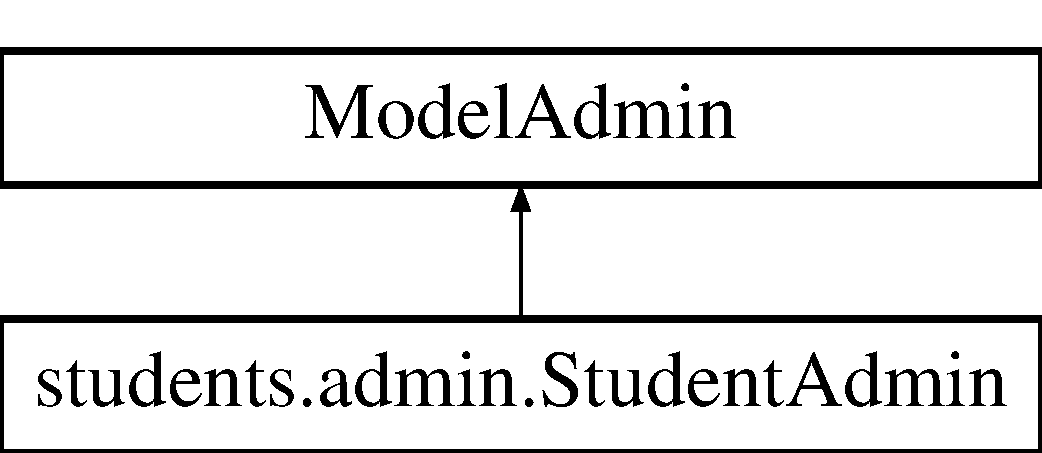
\includegraphics[height=2.000000cm]{classstudents_1_1admin_1_1_student_admin}
\end{center}
\end{figure}
\subsection*{Static Public Attributes}
\begin{DoxyCompactItemize}
\item 
list \hyperlink{classstudents_1_1admin_1_1_student_admin_afbc84f07097db4554415109336880a72}{fieldsets}
\item 
tuple \hyperlink{classstudents_1_1admin_1_1_student_admin_a9d2c7c62d35bba277480bb9333c68ff1}{list\-\_\-display} = ('first\-\_\-name', 'last\-\_\-name', 'institution', 'times\-\_\-logged\-\_\-in')
\item 
list \hyperlink{classstudents_1_1admin_1_1_student_admin_a663d7aee6e08010d1280119d480401a8}{search\-\_\-fields} = \mbox{[}'institution', 'first\-\_\-name'\mbox{]}
\item 
list \hyperlink{classstudents_1_1admin_1_1_student_admin_aa123d7d55ffee26570bf64f62f597a14}{list\-\_\-filter} = \mbox{[}'institution', 'gender', 'times\-\_\-logged\-\_\-in'\mbox{]}
\end{DoxyCompactItemize}


\subsection{Member Data Documentation}
\hypertarget{classstudents_1_1admin_1_1_student_admin_afbc84f07097db4554415109336880a72}{\index{students\-::admin\-::\-Student\-Admin@{students\-::admin\-::\-Student\-Admin}!fieldsets@{fieldsets}}
\index{fieldsets@{fieldsets}!students::admin::StudentAdmin@{students\-::admin\-::\-Student\-Admin}}
\subsubsection[{fieldsets}]{\setlength{\rightskip}{0pt plus 5cm}list students.\-admin.\-Student\-Admin.\-fieldsets\hspace{0.3cm}{\ttfamily [static]}}}\label{classstudents_1_1admin_1_1_student_admin_afbc84f07097db4554415109336880a72}
{\bfseries Initial value\-:}
\begin{DoxyCode}
1 = [
2         (\textcolor{keywordtype}{None}, \{\textcolor{stringliteral}{'fields'}: [\textcolor{stringliteral}{'user'},
3                            \textcolor{stringliteral}{'first\_name'},
4                            \textcolor{stringliteral}{'last\_name'},
5                            \textcolor{stringliteral}{'image'},
6                            \textcolor{stringliteral}{'date\_of\_birth'},
7                            \textcolor{stringliteral}{'gender'},
8                            \textcolor{stringliteral}{'education\_level'},
9                            \textcolor{stringliteral}{'country'},
10                            \textcolor{stringliteral}{'institution'},
11                            \textcolor{stringliteral}{'line\_of\_study'},
12                            \textcolor{stringliteral}{'description'},
13                            \textcolor{stringliteral}{'cv'}
14                            ]\}),
15     ]
\end{DoxyCode}
\hypertarget{classstudents_1_1admin_1_1_student_admin_a9d2c7c62d35bba277480bb9333c68ff1}{\index{students\-::admin\-::\-Student\-Admin@{students\-::admin\-::\-Student\-Admin}!list\-\_\-display@{list\-\_\-display}}
\index{list\-\_\-display@{list\-\_\-display}!students::admin::StudentAdmin@{students\-::admin\-::\-Student\-Admin}}
\subsubsection[{list\-\_\-display}]{\setlength{\rightskip}{0pt plus 5cm}tuple students.\-admin.\-Student\-Admin.\-list\-\_\-display = ('first\-\_\-name', 'last\-\_\-name', 'institution', 'times\-\_\-logged\-\_\-in')\hspace{0.3cm}{\ttfamily [static]}}}\label{classstudents_1_1admin_1_1_student_admin_a9d2c7c62d35bba277480bb9333c68ff1}
\hypertarget{classstudents_1_1admin_1_1_student_admin_aa123d7d55ffee26570bf64f62f597a14}{\index{students\-::admin\-::\-Student\-Admin@{students\-::admin\-::\-Student\-Admin}!list\-\_\-filter@{list\-\_\-filter}}
\index{list\-\_\-filter@{list\-\_\-filter}!students::admin::StudentAdmin@{students\-::admin\-::\-Student\-Admin}}
\subsubsection[{list\-\_\-filter}]{\setlength{\rightskip}{0pt plus 5cm}list students.\-admin.\-Student\-Admin.\-list\-\_\-filter = \mbox{[}'institution', 'gender', 'times\-\_\-logged\-\_\-in'\mbox{]}\hspace{0.3cm}{\ttfamily [static]}}}\label{classstudents_1_1admin_1_1_student_admin_aa123d7d55ffee26570bf64f62f597a14}
\hypertarget{classstudents_1_1admin_1_1_student_admin_a663d7aee6e08010d1280119d480401a8}{\index{students\-::admin\-::\-Student\-Admin@{students\-::admin\-::\-Student\-Admin}!search\-\_\-fields@{search\-\_\-fields}}
\index{search\-\_\-fields@{search\-\_\-fields}!students::admin::StudentAdmin@{students\-::admin\-::\-Student\-Admin}}
\subsubsection[{search\-\_\-fields}]{\setlength{\rightskip}{0pt plus 5cm}list students.\-admin.\-Student\-Admin.\-search\-\_\-fields = \mbox{[}'institution', 'first\-\_\-name'\mbox{]}\hspace{0.3cm}{\ttfamily [static]}}}\label{classstudents_1_1admin_1_1_student_admin_a663d7aee6e08010d1280119d480401a8}


The documentation for this class was generated from the following file\-:\begin{DoxyCompactItemize}
\item 
leapkit/students/\hyperlink{admin_8py}{admin.\-py}\end{DoxyCompactItemize}

\hypertarget{classstudents_1_1forms_1_1_student_creation_form}{\section{students.\-forms.\-Student\-Creation\-Form Class Reference}
\label{classstudents_1_1forms_1_1_student_creation_form}\index{students.\-forms.\-Student\-Creation\-Form@{students.\-forms.\-Student\-Creation\-Form}}
}
Inheritance diagram for students.\-forms.\-Student\-Creation\-Form\-:\begin{figure}[H]
\begin{center}
\leavevmode
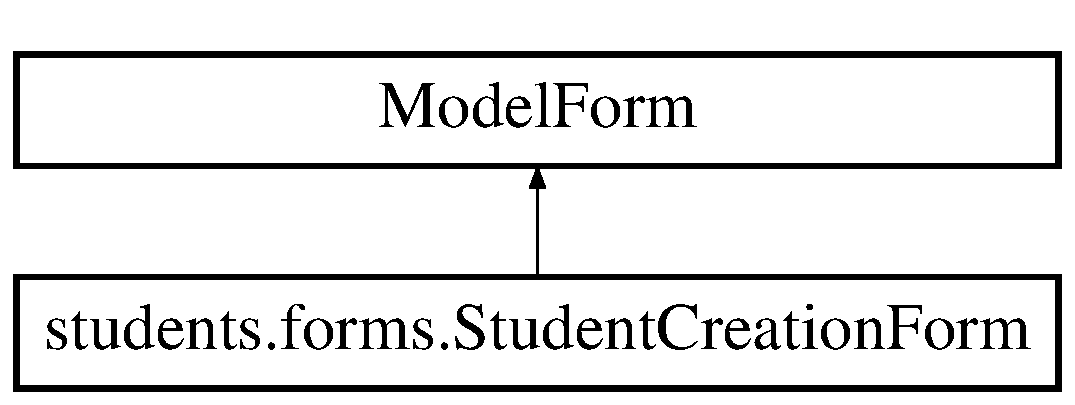
\includegraphics[height=2.000000cm]{classstudents_1_1forms_1_1_student_creation_form}
\end{center}
\end{figure}
\subsection*{Classes}
\begin{DoxyCompactItemize}
\item 
class \hyperlink{classstudents_1_1forms_1_1_student_creation_form_1_1_meta}{Meta}
\end{DoxyCompactItemize}
\subsection*{Public Member Functions}
\begin{DoxyCompactItemize}
\item 
def \hyperlink{classstudents_1_1forms_1_1_student_creation_form_a354056c98aeeab7ca25a38c804a814b0}{\-\_\-\-\_\-init\-\_\-\-\_\-}
\item 
def \hyperlink{classstudents_1_1forms_1_1_student_creation_form_ab526befbe262db07ff883fa1d116fb2c}{clean\-\_\-email}
\item 
def \hyperlink{classstudents_1_1forms_1_1_student_creation_form_a22e51e371db82bea72497d7b7a6a2dd5}{clean\-\_\-password2}
\item 
def \hyperlink{classstudents_1_1forms_1_1_student_creation_form_a2bb73432d2899324260b1e426520ffa7}{save}
\end{DoxyCompactItemize}
\subsection*{Public Attributes}
\begin{DoxyCompactItemize}
\item 
\hyperlink{classstudents_1_1forms_1_1_student_creation_form_ae1155eb425b3d6d3367af8f8f09dc239}{helper}
\end{DoxyCompactItemize}
\subsection*{Static Public Attributes}
\begin{DoxyCompactItemize}
\item 
tuple \hyperlink{classstudents_1_1forms_1_1_student_creation_form_a6a1bb012c88fcfa09027ca6e951a7ae3}{email} = forms.\-Email\-Field(required=True)
\item 
tuple \hyperlink{classstudents_1_1forms_1_1_student_creation_form_a5386136d5fa960ed2b47baaeedfa4e7d}{password1} = forms.\-Char\-Field(required=True, widget=forms.\-Password\-Input())
\item 
tuple \hyperlink{classstudents_1_1forms_1_1_student_creation_form_a80b36a4c23794bf568774c3fd915351b}{password2} = forms.\-Char\-Field(required=True, widget=forms.\-Password\-Input())
\end{DoxyCompactItemize}


\subsection{Constructor \& Destructor Documentation}
\hypertarget{classstudents_1_1forms_1_1_student_creation_form_a354056c98aeeab7ca25a38c804a814b0}{\index{students\-::forms\-::\-Student\-Creation\-Form@{students\-::forms\-::\-Student\-Creation\-Form}!\-\_\-\-\_\-init\-\_\-\-\_\-@{\-\_\-\-\_\-init\-\_\-\-\_\-}}
\index{\-\_\-\-\_\-init\-\_\-\-\_\-@{\-\_\-\-\_\-init\-\_\-\-\_\-}!students::forms::StudentCreationForm@{students\-::forms\-::\-Student\-Creation\-Form}}
\subsubsection[{\-\_\-\-\_\-init\-\_\-\-\_\-}]{\setlength{\rightskip}{0pt plus 5cm}def students.\-forms.\-Student\-Creation\-Form.\-\_\-\-\_\-init\-\_\-\-\_\- (
\begin{DoxyParamCaption}
\item[{}]{self, }
\item[{}]{args, }
\item[{}]{kwargs}
\end{DoxyParamCaption}
)}}\label{classstudents_1_1forms_1_1_student_creation_form_a354056c98aeeab7ca25a38c804a814b0}


\subsection{Member Function Documentation}
\hypertarget{classstudents_1_1forms_1_1_student_creation_form_ab526befbe262db07ff883fa1d116fb2c}{\index{students\-::forms\-::\-Student\-Creation\-Form@{students\-::forms\-::\-Student\-Creation\-Form}!clean\-\_\-email@{clean\-\_\-email}}
\index{clean\-\_\-email@{clean\-\_\-email}!students::forms::StudentCreationForm@{students\-::forms\-::\-Student\-Creation\-Form}}
\subsubsection[{clean\-\_\-email}]{\setlength{\rightskip}{0pt plus 5cm}def students.\-forms.\-Student\-Creation\-Form.\-clean\-\_\-email (
\begin{DoxyParamCaption}
\item[{}]{self}
\end{DoxyParamCaption}
)}}\label{classstudents_1_1forms_1_1_student_creation_form_ab526befbe262db07ff883fa1d116fb2c}
\hypertarget{classstudents_1_1forms_1_1_student_creation_form_a22e51e371db82bea72497d7b7a6a2dd5}{\index{students\-::forms\-::\-Student\-Creation\-Form@{students\-::forms\-::\-Student\-Creation\-Form}!clean\-\_\-password2@{clean\-\_\-password2}}
\index{clean\-\_\-password2@{clean\-\_\-password2}!students::forms::StudentCreationForm@{students\-::forms\-::\-Student\-Creation\-Form}}
\subsubsection[{clean\-\_\-password2}]{\setlength{\rightskip}{0pt plus 5cm}def students.\-forms.\-Student\-Creation\-Form.\-clean\-\_\-password2 (
\begin{DoxyParamCaption}
\item[{}]{self}
\end{DoxyParamCaption}
)}}\label{classstudents_1_1forms_1_1_student_creation_form_a22e51e371db82bea72497d7b7a6a2dd5}
\hypertarget{classstudents_1_1forms_1_1_student_creation_form_a2bb73432d2899324260b1e426520ffa7}{\index{students\-::forms\-::\-Student\-Creation\-Form@{students\-::forms\-::\-Student\-Creation\-Form}!save@{save}}
\index{save@{save}!students::forms::StudentCreationForm@{students\-::forms\-::\-Student\-Creation\-Form}}
\subsubsection[{save}]{\setlength{\rightskip}{0pt plus 5cm}def students.\-forms.\-Student\-Creation\-Form.\-save (
\begin{DoxyParamCaption}
\item[{}]{self, }
\item[{}]{commit = {\ttfamily True}}
\end{DoxyParamCaption}
)}}\label{classstudents_1_1forms_1_1_student_creation_form_a2bb73432d2899324260b1e426520ffa7}


\subsection{Member Data Documentation}
\hypertarget{classstudents_1_1forms_1_1_student_creation_form_a6a1bb012c88fcfa09027ca6e951a7ae3}{\index{students\-::forms\-::\-Student\-Creation\-Form@{students\-::forms\-::\-Student\-Creation\-Form}!email@{email}}
\index{email@{email}!students::forms::StudentCreationForm@{students\-::forms\-::\-Student\-Creation\-Form}}
\subsubsection[{email}]{\setlength{\rightskip}{0pt plus 5cm}tuple students.\-forms.\-Student\-Creation\-Form.\-email = forms.\-Email\-Field(required=True)\hspace{0.3cm}{\ttfamily [static]}}}\label{classstudents_1_1forms_1_1_student_creation_form_a6a1bb012c88fcfa09027ca6e951a7ae3}
\hypertarget{classstudents_1_1forms_1_1_student_creation_form_ae1155eb425b3d6d3367af8f8f09dc239}{\index{students\-::forms\-::\-Student\-Creation\-Form@{students\-::forms\-::\-Student\-Creation\-Form}!helper@{helper}}
\index{helper@{helper}!students::forms::StudentCreationForm@{students\-::forms\-::\-Student\-Creation\-Form}}
\subsubsection[{helper}]{\setlength{\rightskip}{0pt plus 5cm}students.\-forms.\-Student\-Creation\-Form.\-helper}}\label{classstudents_1_1forms_1_1_student_creation_form_ae1155eb425b3d6d3367af8f8f09dc239}
\hypertarget{classstudents_1_1forms_1_1_student_creation_form_a5386136d5fa960ed2b47baaeedfa4e7d}{\index{students\-::forms\-::\-Student\-Creation\-Form@{students\-::forms\-::\-Student\-Creation\-Form}!password1@{password1}}
\index{password1@{password1}!students::forms::StudentCreationForm@{students\-::forms\-::\-Student\-Creation\-Form}}
\subsubsection[{password1}]{\setlength{\rightskip}{0pt plus 5cm}tuple students.\-forms.\-Student\-Creation\-Form.\-password1 = forms.\-Char\-Field(required=True, widget=forms.\-Password\-Input())\hspace{0.3cm}{\ttfamily [static]}}}\label{classstudents_1_1forms_1_1_student_creation_form_a5386136d5fa960ed2b47baaeedfa4e7d}
\hypertarget{classstudents_1_1forms_1_1_student_creation_form_a80b36a4c23794bf568774c3fd915351b}{\index{students\-::forms\-::\-Student\-Creation\-Form@{students\-::forms\-::\-Student\-Creation\-Form}!password2@{password2}}
\index{password2@{password2}!students::forms::StudentCreationForm@{students\-::forms\-::\-Student\-Creation\-Form}}
\subsubsection[{password2}]{\setlength{\rightskip}{0pt plus 5cm}tuple students.\-forms.\-Student\-Creation\-Form.\-password2 = forms.\-Char\-Field(required=True, widget=forms.\-Password\-Input())\hspace{0.3cm}{\ttfamily [static]}}}\label{classstudents_1_1forms_1_1_student_creation_form_a80b36a4c23794bf568774c3fd915351b}


The documentation for this class was generated from the following file\-:\begin{DoxyCompactItemize}
\item 
leapkit/students/\hyperlink{forms_8py}{forms.\-py}\end{DoxyCompactItemize}

\hypertarget{classstudents_1_1views_1_1_student_f_a_q_view}{\section{students.\-views.\-Student\-F\-A\-Q\-View Class Reference}
\label{classstudents_1_1views_1_1_student_f_a_q_view}\index{students.\-views.\-Student\-F\-A\-Q\-View@{students.\-views.\-Student\-F\-A\-Q\-View}}
}
Inheritance diagram for students.\-views.\-Student\-F\-A\-Q\-View\-:\begin{figure}[H]
\begin{center}
\leavevmode
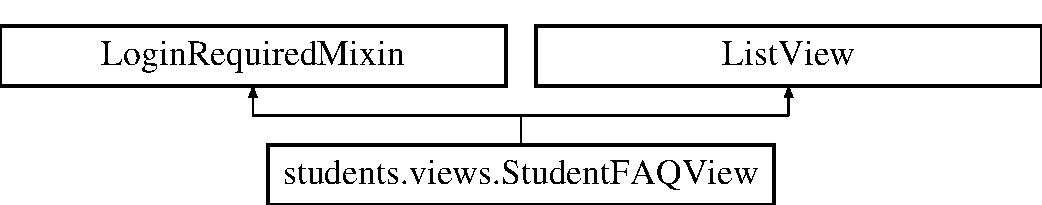
\includegraphics[height=2.000000cm]{classstudents_1_1views_1_1_student_f_a_q_view}
\end{center}
\end{figure}
\subsection*{Public Member Functions}
\begin{DoxyCompactItemize}
\item 
def \hyperlink{classstudents_1_1views_1_1_student_f_a_q_view_ab7a8f396a3327b1aec9bbaf3e28efb9e}{get\-\_\-queryset}
\end{DoxyCompactItemize}
\subsection*{Static Public Attributes}
\begin{DoxyCompactItemize}
\item 
string \hyperlink{classstudents_1_1views_1_1_student_f_a_q_view_a15ab67fe5f4e7cdfcdca7459dbc3c8df}{template\-\_\-name} = \char`\"{}students\-\_\-\-F\-A\-Q\-\_\-view.\-html\char`\"{}
\item 
string \hyperlink{classstudents_1_1views_1_1_student_f_a_q_view_a187c58fd089481cf81e7bbb14e0c65bd}{login\-\_\-url} = \char`\"{}/students/login/\char`\"{}
\item 
\hyperlink{classstudents_1_1views_1_1_student_f_a_q_view_a4bf4e4cb8a13b7d970373e37fe67ce74}{model} = F\-A\-Question
\end{DoxyCompactItemize}


\subsection{Member Function Documentation}
\hypertarget{classstudents_1_1views_1_1_student_f_a_q_view_ab7a8f396a3327b1aec9bbaf3e28efb9e}{\index{students\-::views\-::\-Student\-F\-A\-Q\-View@{students\-::views\-::\-Student\-F\-A\-Q\-View}!get\-\_\-queryset@{get\-\_\-queryset}}
\index{get\-\_\-queryset@{get\-\_\-queryset}!students::views::StudentFAQView@{students\-::views\-::\-Student\-F\-A\-Q\-View}}
\subsubsection[{get\-\_\-queryset}]{\setlength{\rightskip}{0pt plus 5cm}def students.\-views.\-Student\-F\-A\-Q\-View.\-get\-\_\-queryset (
\begin{DoxyParamCaption}
\item[{}]{self}
\end{DoxyParamCaption}
)}}\label{classstudents_1_1views_1_1_student_f_a_q_view_ab7a8f396a3327b1aec9bbaf3e28efb9e}


\subsection{Member Data Documentation}
\hypertarget{classstudents_1_1views_1_1_student_f_a_q_view_a187c58fd089481cf81e7bbb14e0c65bd}{\index{students\-::views\-::\-Student\-F\-A\-Q\-View@{students\-::views\-::\-Student\-F\-A\-Q\-View}!login\-\_\-url@{login\-\_\-url}}
\index{login\-\_\-url@{login\-\_\-url}!students::views::StudentFAQView@{students\-::views\-::\-Student\-F\-A\-Q\-View}}
\subsubsection[{login\-\_\-url}]{\setlength{\rightskip}{0pt plus 5cm}string students.\-views.\-Student\-F\-A\-Q\-View.\-login\-\_\-url = \char`\"{}/students/login/\char`\"{}\hspace{0.3cm}{\ttfamily [static]}}}\label{classstudents_1_1views_1_1_student_f_a_q_view_a187c58fd089481cf81e7bbb14e0c65bd}
\hypertarget{classstudents_1_1views_1_1_student_f_a_q_view_a4bf4e4cb8a13b7d970373e37fe67ce74}{\index{students\-::views\-::\-Student\-F\-A\-Q\-View@{students\-::views\-::\-Student\-F\-A\-Q\-View}!model@{model}}
\index{model@{model}!students::views::StudentFAQView@{students\-::views\-::\-Student\-F\-A\-Q\-View}}
\subsubsection[{model}]{\setlength{\rightskip}{0pt plus 5cm}students.\-views.\-Student\-F\-A\-Q\-View.\-model = F\-A\-Question\hspace{0.3cm}{\ttfamily [static]}}}\label{classstudents_1_1views_1_1_student_f_a_q_view_a4bf4e4cb8a13b7d970373e37fe67ce74}
\hypertarget{classstudents_1_1views_1_1_student_f_a_q_view_a15ab67fe5f4e7cdfcdca7459dbc3c8df}{\index{students\-::views\-::\-Student\-F\-A\-Q\-View@{students\-::views\-::\-Student\-F\-A\-Q\-View}!template\-\_\-name@{template\-\_\-name}}
\index{template\-\_\-name@{template\-\_\-name}!students::views::StudentFAQView@{students\-::views\-::\-Student\-F\-A\-Q\-View}}
\subsubsection[{template\-\_\-name}]{\setlength{\rightskip}{0pt plus 5cm}string students.\-views.\-Student\-F\-A\-Q\-View.\-template\-\_\-name = \char`\"{}students\-\_\-\-F\-A\-Q\-\_\-view.\-html\char`\"{}\hspace{0.3cm}{\ttfamily [static]}}}\label{classstudents_1_1views_1_1_student_f_a_q_view_a15ab67fe5f4e7cdfcdca7459dbc3c8df}


The documentation for this class was generated from the following file\-:\begin{DoxyCompactItemize}
\item 
leapkit/students/\hyperlink{views_8py}{views.\-py}\end{DoxyCompactItemize}

\hypertarget{classstudents_1_1views_1_1_student_feed_back}{\section{students.\-views.\-Student\-Feed\-Back Class Reference}
\label{classstudents_1_1views_1_1_student_feed_back}\index{students.\-views.\-Student\-Feed\-Back@{students.\-views.\-Student\-Feed\-Back}}
}
Inheritance diagram for students.\-views.\-Student\-Feed\-Back\-:\begin{figure}[H]
\begin{center}
\leavevmode
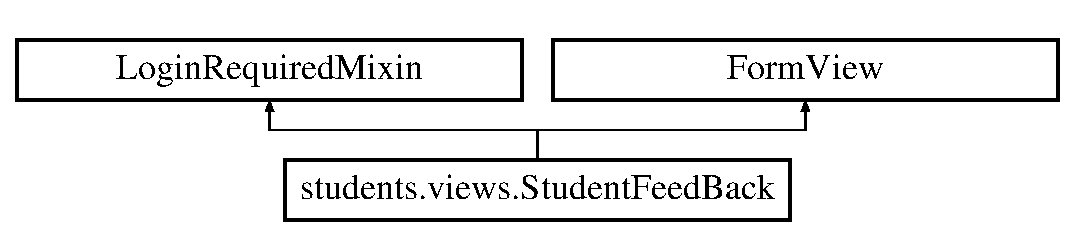
\includegraphics[height=2.000000cm]{classstudents_1_1views_1_1_student_feed_back}
\end{center}
\end{figure}
\subsection*{Public Member Functions}
\begin{DoxyCompactItemize}
\item 
def \hyperlink{classstudents_1_1views_1_1_student_feed_back_afc5508fe4ca2258556fd31eb7d680694}{form\-\_\-valid}
\item 
def \hyperlink{classstudents_1_1views_1_1_student_feed_back_ab65735dbdc4a51b5fde3228afb3cb062}{form\-\_\-invalid}
\end{DoxyCompactItemize}
\subsection*{Static Public Attributes}
\begin{DoxyCompactItemize}
\item 
string \hyperlink{classstudents_1_1views_1_1_student_feed_back_aba4fdf3ecec134b999393bbd6d402a25}{template\-\_\-name} = \char`\"{}student\-\_\-feedback.\-html\char`\"{}
\item 
string \hyperlink{classstudents_1_1views_1_1_student_feed_back_a1252dc07438b7d8230a4f516e7a52af6}{login\-\_\-url} = \char`\"{}/students/login/\char`\"{}
\item 
\hyperlink{classstudents_1_1views_1_1_student_feed_back_a94d1baf728a44c115ea4950a0caefbce}{model} = User\-Question
\item 
\hyperlink{classstudents_1_1views_1_1_student_feed_back_a98fa33feb41e0851cda2e65f112d4105}{form\-\_\-class} = Contact\-Form
\end{DoxyCompactItemize}


\subsection{Member Function Documentation}
\hypertarget{classstudents_1_1views_1_1_student_feed_back_ab65735dbdc4a51b5fde3228afb3cb062}{\index{students\-::views\-::\-Student\-Feed\-Back@{students\-::views\-::\-Student\-Feed\-Back}!form\-\_\-invalid@{form\-\_\-invalid}}
\index{form\-\_\-invalid@{form\-\_\-invalid}!students::views::StudentFeedBack@{students\-::views\-::\-Student\-Feed\-Back}}
\subsubsection[{form\-\_\-invalid}]{\setlength{\rightskip}{0pt plus 5cm}def students.\-views.\-Student\-Feed\-Back.\-form\-\_\-invalid (
\begin{DoxyParamCaption}
\item[{}]{self, }
\item[{}]{form}
\end{DoxyParamCaption}
)}}\label{classstudents_1_1views_1_1_student_feed_back_ab65735dbdc4a51b5fde3228afb3cb062}
\hypertarget{classstudents_1_1views_1_1_student_feed_back_afc5508fe4ca2258556fd31eb7d680694}{\index{students\-::views\-::\-Student\-Feed\-Back@{students\-::views\-::\-Student\-Feed\-Back}!form\-\_\-valid@{form\-\_\-valid}}
\index{form\-\_\-valid@{form\-\_\-valid}!students::views::StudentFeedBack@{students\-::views\-::\-Student\-Feed\-Back}}
\subsubsection[{form\-\_\-valid}]{\setlength{\rightskip}{0pt plus 5cm}def students.\-views.\-Student\-Feed\-Back.\-form\-\_\-valid (
\begin{DoxyParamCaption}
\item[{}]{self, }
\item[{}]{form}
\end{DoxyParamCaption}
)}}\label{classstudents_1_1views_1_1_student_feed_back_afc5508fe4ca2258556fd31eb7d680694}


\subsection{Member Data Documentation}
\hypertarget{classstudents_1_1views_1_1_student_feed_back_a98fa33feb41e0851cda2e65f112d4105}{\index{students\-::views\-::\-Student\-Feed\-Back@{students\-::views\-::\-Student\-Feed\-Back}!form\-\_\-class@{form\-\_\-class}}
\index{form\-\_\-class@{form\-\_\-class}!students::views::StudentFeedBack@{students\-::views\-::\-Student\-Feed\-Back}}
\subsubsection[{form\-\_\-class}]{\setlength{\rightskip}{0pt plus 5cm}students.\-views.\-Student\-Feed\-Back.\-form\-\_\-class = Contact\-Form\hspace{0.3cm}{\ttfamily [static]}}}\label{classstudents_1_1views_1_1_student_feed_back_a98fa33feb41e0851cda2e65f112d4105}
\hypertarget{classstudents_1_1views_1_1_student_feed_back_a1252dc07438b7d8230a4f516e7a52af6}{\index{students\-::views\-::\-Student\-Feed\-Back@{students\-::views\-::\-Student\-Feed\-Back}!login\-\_\-url@{login\-\_\-url}}
\index{login\-\_\-url@{login\-\_\-url}!students::views::StudentFeedBack@{students\-::views\-::\-Student\-Feed\-Back}}
\subsubsection[{login\-\_\-url}]{\setlength{\rightskip}{0pt plus 5cm}string students.\-views.\-Student\-Feed\-Back.\-login\-\_\-url = \char`\"{}/students/login/\char`\"{}\hspace{0.3cm}{\ttfamily [static]}}}\label{classstudents_1_1views_1_1_student_feed_back_a1252dc07438b7d8230a4f516e7a52af6}
\hypertarget{classstudents_1_1views_1_1_student_feed_back_a94d1baf728a44c115ea4950a0caefbce}{\index{students\-::views\-::\-Student\-Feed\-Back@{students\-::views\-::\-Student\-Feed\-Back}!model@{model}}
\index{model@{model}!students::views::StudentFeedBack@{students\-::views\-::\-Student\-Feed\-Back}}
\subsubsection[{model}]{\setlength{\rightskip}{0pt plus 5cm}students.\-views.\-Student\-Feed\-Back.\-model = User\-Question\hspace{0.3cm}{\ttfamily [static]}}}\label{classstudents_1_1views_1_1_student_feed_back_a94d1baf728a44c115ea4950a0caefbce}
\hypertarget{classstudents_1_1views_1_1_student_feed_back_aba4fdf3ecec134b999393bbd6d402a25}{\index{students\-::views\-::\-Student\-Feed\-Back@{students\-::views\-::\-Student\-Feed\-Back}!template\-\_\-name@{template\-\_\-name}}
\index{template\-\_\-name@{template\-\_\-name}!students::views::StudentFeedBack@{students\-::views\-::\-Student\-Feed\-Back}}
\subsubsection[{template\-\_\-name}]{\setlength{\rightskip}{0pt plus 5cm}string students.\-views.\-Student\-Feed\-Back.\-template\-\_\-name = \char`\"{}student\-\_\-feedback.\-html\char`\"{}\hspace{0.3cm}{\ttfamily [static]}}}\label{classstudents_1_1views_1_1_student_feed_back_aba4fdf3ecec134b999393bbd6d402a25}


The documentation for this class was generated from the following file\-:\begin{DoxyCompactItemize}
\item 
leapkit/students/\hyperlink{views_8py}{views.\-py}\end{DoxyCompactItemize}

\hypertarget{classstudents_1_1forms_1_1_student_form}{\section{students.\-forms.\-Student\-Form Class Reference}
\label{classstudents_1_1forms_1_1_student_form}\index{students.\-forms.\-Student\-Form@{students.\-forms.\-Student\-Form}}
}
Inheritance diagram for students.\-forms.\-Student\-Form\-:\begin{figure}[H]
\begin{center}
\leavevmode
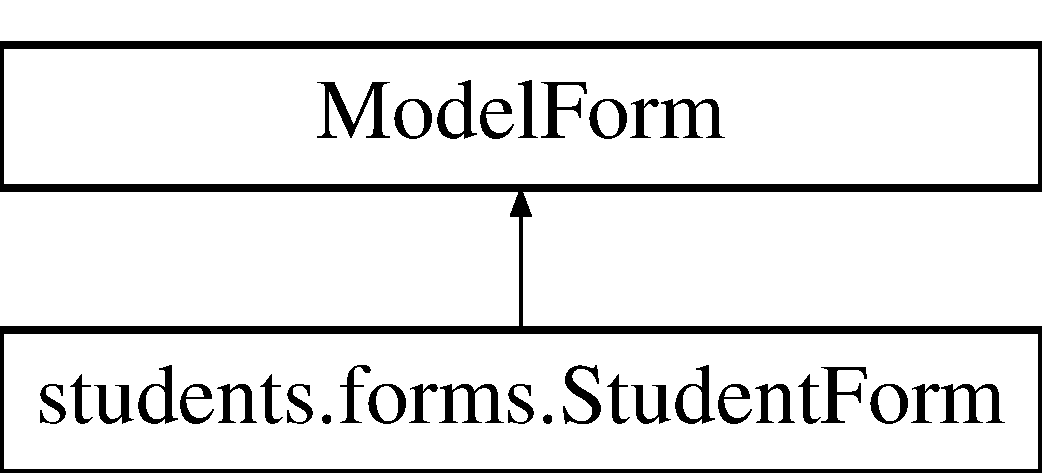
\includegraphics[height=2.000000cm]{classstudents_1_1forms_1_1_student_form}
\end{center}
\end{figure}
\subsection*{Classes}
\begin{DoxyCompactItemize}
\item 
class \hyperlink{classstudents_1_1forms_1_1_student_form_1_1_meta}{Meta}
\end{DoxyCompactItemize}
\subsection*{Public Member Functions}
\begin{DoxyCompactItemize}
\item 
def \hyperlink{classstudents_1_1forms_1_1_student_form_a2cfb0cfcdd792efec48f8936f8289365}{\-\_\-\-\_\-init\-\_\-\-\_\-}
\end{DoxyCompactItemize}
\subsection*{Public Attributes}
\begin{DoxyCompactItemize}
\item 
\hyperlink{classstudents_1_1forms_1_1_student_form_a4a28a9682e6d190c1957fb9fb29fdb0e}{helper}
\end{DoxyCompactItemize}


\subsection{Constructor \& Destructor Documentation}
\hypertarget{classstudents_1_1forms_1_1_student_form_a2cfb0cfcdd792efec48f8936f8289365}{\index{students\-::forms\-::\-Student\-Form@{students\-::forms\-::\-Student\-Form}!\-\_\-\-\_\-init\-\_\-\-\_\-@{\-\_\-\-\_\-init\-\_\-\-\_\-}}
\index{\-\_\-\-\_\-init\-\_\-\-\_\-@{\-\_\-\-\_\-init\-\_\-\-\_\-}!students::forms::StudentForm@{students\-::forms\-::\-Student\-Form}}
\subsubsection[{\-\_\-\-\_\-init\-\_\-\-\_\-}]{\setlength{\rightskip}{0pt plus 5cm}def students.\-forms.\-Student\-Form.\-\_\-\-\_\-init\-\_\-\-\_\- (
\begin{DoxyParamCaption}
\item[{}]{self, }
\item[{}]{args, }
\item[{}]{kwargs}
\end{DoxyParamCaption}
)}}\label{classstudents_1_1forms_1_1_student_form_a2cfb0cfcdd792efec48f8936f8289365}


\subsection{Member Data Documentation}
\hypertarget{classstudents_1_1forms_1_1_student_form_a4a28a9682e6d190c1957fb9fb29fdb0e}{\index{students\-::forms\-::\-Student\-Form@{students\-::forms\-::\-Student\-Form}!helper@{helper}}
\index{helper@{helper}!students::forms::StudentForm@{students\-::forms\-::\-Student\-Form}}
\subsubsection[{helper}]{\setlength{\rightskip}{0pt plus 5cm}students.\-forms.\-Student\-Form.\-helper}}\label{classstudents_1_1forms_1_1_student_form_a4a28a9682e6d190c1957fb9fb29fdb0e}


The documentation for this class was generated from the following file\-:\begin{DoxyCompactItemize}
\item 
leapkit/students/\hyperlink{forms_8py}{forms.\-py}\end{DoxyCompactItemize}

\hypertarget{classstudents_1_1forms_1_1_student_log_in_form}{\section{students.\-forms.\-Student\-Log\-In\-Form Class Reference}
\label{classstudents_1_1forms_1_1_student_log_in_form}\index{students.\-forms.\-Student\-Log\-In\-Form@{students.\-forms.\-Student\-Log\-In\-Form}}
}
Inheritance diagram for students.\-forms.\-Student\-Log\-In\-Form\-:\begin{figure}[H]
\begin{center}
\leavevmode
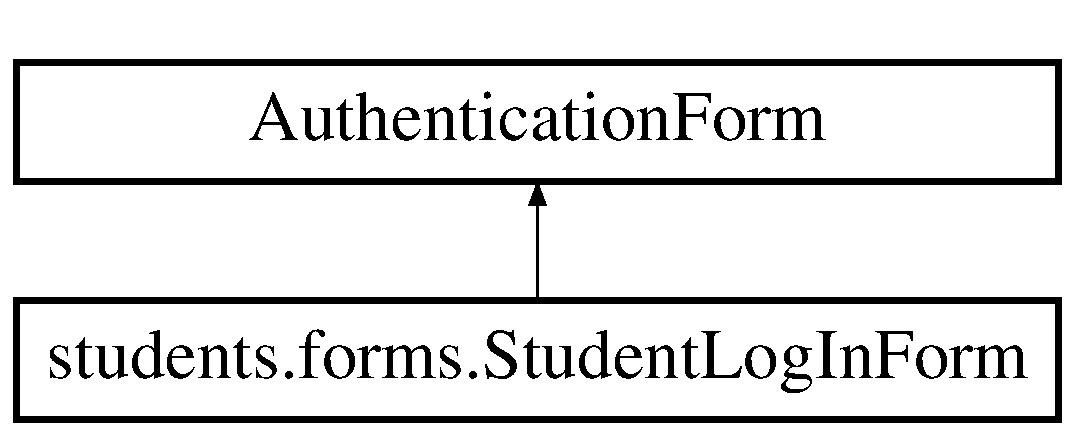
\includegraphics[height=2.000000cm]{classstudents_1_1forms_1_1_student_log_in_form}
\end{center}
\end{figure}
\subsection*{Classes}
\begin{DoxyCompactItemize}
\item 
class \hyperlink{classstudents_1_1forms_1_1_student_log_in_form_1_1_meta}{Meta}
\end{DoxyCompactItemize}
\subsection*{Public Member Functions}
\begin{DoxyCompactItemize}
\item 
def \hyperlink{classstudents_1_1forms_1_1_student_log_in_form_a00a3aca2c23b93a806a8e0a908e5cd14}{\-\_\-\-\_\-init\-\_\-\-\_\-}
\end{DoxyCompactItemize}
\subsection*{Public Attributes}
\begin{DoxyCompactItemize}
\item 
\hyperlink{classstudents_1_1forms_1_1_student_log_in_form_a326cea774299d9fa1e8bcf89644c7c49}{helper}
\end{DoxyCompactItemize}


\subsection{Constructor \& Destructor Documentation}
\hypertarget{classstudents_1_1forms_1_1_student_log_in_form_a00a3aca2c23b93a806a8e0a908e5cd14}{\index{students\-::forms\-::\-Student\-Log\-In\-Form@{students\-::forms\-::\-Student\-Log\-In\-Form}!\-\_\-\-\_\-init\-\_\-\-\_\-@{\-\_\-\-\_\-init\-\_\-\-\_\-}}
\index{\-\_\-\-\_\-init\-\_\-\-\_\-@{\-\_\-\-\_\-init\-\_\-\-\_\-}!students::forms::StudentLogInForm@{students\-::forms\-::\-Student\-Log\-In\-Form}}
\subsubsection[{\-\_\-\-\_\-init\-\_\-\-\_\-}]{\setlength{\rightskip}{0pt plus 5cm}def students.\-forms.\-Student\-Log\-In\-Form.\-\_\-\-\_\-init\-\_\-\-\_\- (
\begin{DoxyParamCaption}
\item[{}]{self, }
\item[{}]{args, }
\item[{}]{kwargs}
\end{DoxyParamCaption}
)}}\label{classstudents_1_1forms_1_1_student_log_in_form_a00a3aca2c23b93a806a8e0a908e5cd14}


\subsection{Member Data Documentation}
\hypertarget{classstudents_1_1forms_1_1_student_log_in_form_a326cea774299d9fa1e8bcf89644c7c49}{\index{students\-::forms\-::\-Student\-Log\-In\-Form@{students\-::forms\-::\-Student\-Log\-In\-Form}!helper@{helper}}
\index{helper@{helper}!students::forms::StudentLogInForm@{students\-::forms\-::\-Student\-Log\-In\-Form}}
\subsubsection[{helper}]{\setlength{\rightskip}{0pt plus 5cm}students.\-forms.\-Student\-Log\-In\-Form.\-helper}}\label{classstudents_1_1forms_1_1_student_log_in_form_a326cea774299d9fa1e8bcf89644c7c49}


The documentation for this class was generated from the following file\-:\begin{DoxyCompactItemize}
\item 
leapkit/students/\hyperlink{forms_8py}{forms.\-py}\end{DoxyCompactItemize}

\hypertarget{classstudents_1_1views_1_1_student_log_in_view}{\section{students.\-views.\-Student\-Log\-In\-View Class Reference}
\label{classstudents_1_1views_1_1_student_log_in_view}\index{students.\-views.\-Student\-Log\-In\-View@{students.\-views.\-Student\-Log\-In\-View}}
}
Inheritance diagram for students.\-views.\-Student\-Log\-In\-View\-:\begin{figure}[H]
\begin{center}
\leavevmode
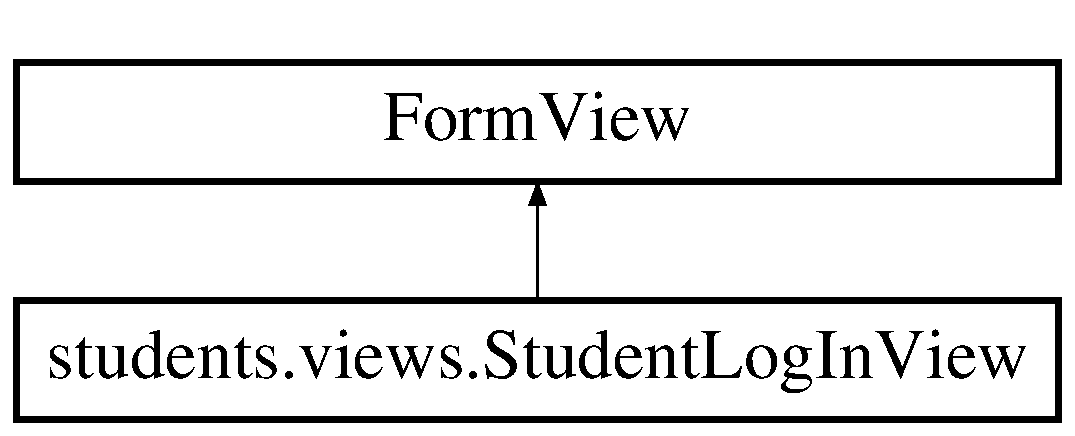
\includegraphics[height=2.000000cm]{classstudents_1_1views_1_1_student_log_in_view}
\end{center}
\end{figure}
\subsection*{Public Member Functions}
\begin{DoxyCompactItemize}
\item 
def \hyperlink{classstudents_1_1views_1_1_student_log_in_view_a090cfaafcae5b8aae1a89fbbd2325b63}{form\-\_\-valid}
\item 
def \hyperlink{classstudents_1_1views_1_1_student_log_in_view_a366b874458816a4940268304c2096fca}{form\-\_\-invalid}
\end{DoxyCompactItemize}
\subsection*{Static Public Attributes}
\begin{DoxyCompactItemize}
\item 
string \hyperlink{classstudents_1_1views_1_1_student_log_in_view_a6c533a74b8b7c2eab25e8e357aed18be}{template\-\_\-name} = \char`\"{}student\-\_\-log\-\_\-in.\-html\char`\"{}
\item 
\hyperlink{classstudents_1_1views_1_1_student_log_in_view_a3e3e16f553aee428f087b669da95ada0}{form\-\_\-class} = Student\-Log\-In\-Form
\item 
\hyperlink{classstudents_1_1views_1_1_student_log_in_view_a5acd7d5724d7a6cbc0963424420c4f5e}{model} = User
\end{DoxyCompactItemize}


\subsection{Member Function Documentation}
\hypertarget{classstudents_1_1views_1_1_student_log_in_view_a366b874458816a4940268304c2096fca}{\index{students\-::views\-::\-Student\-Log\-In\-View@{students\-::views\-::\-Student\-Log\-In\-View}!form\-\_\-invalid@{form\-\_\-invalid}}
\index{form\-\_\-invalid@{form\-\_\-invalid}!students::views::StudentLogInView@{students\-::views\-::\-Student\-Log\-In\-View}}
\subsubsection[{form\-\_\-invalid}]{\setlength{\rightskip}{0pt plus 5cm}def students.\-views.\-Student\-Log\-In\-View.\-form\-\_\-invalid (
\begin{DoxyParamCaption}
\item[{}]{self, }
\item[{}]{form}
\end{DoxyParamCaption}
)}}\label{classstudents_1_1views_1_1_student_log_in_view_a366b874458816a4940268304c2096fca}
\hypertarget{classstudents_1_1views_1_1_student_log_in_view_a090cfaafcae5b8aae1a89fbbd2325b63}{\index{students\-::views\-::\-Student\-Log\-In\-View@{students\-::views\-::\-Student\-Log\-In\-View}!form\-\_\-valid@{form\-\_\-valid}}
\index{form\-\_\-valid@{form\-\_\-valid}!students::views::StudentLogInView@{students\-::views\-::\-Student\-Log\-In\-View}}
\subsubsection[{form\-\_\-valid}]{\setlength{\rightskip}{0pt plus 5cm}def students.\-views.\-Student\-Log\-In\-View.\-form\-\_\-valid (
\begin{DoxyParamCaption}
\item[{}]{self, }
\item[{}]{form}
\end{DoxyParamCaption}
)}}\label{classstudents_1_1views_1_1_student_log_in_view_a090cfaafcae5b8aae1a89fbbd2325b63}


\subsection{Member Data Documentation}
\hypertarget{classstudents_1_1views_1_1_student_log_in_view_a3e3e16f553aee428f087b669da95ada0}{\index{students\-::views\-::\-Student\-Log\-In\-View@{students\-::views\-::\-Student\-Log\-In\-View}!form\-\_\-class@{form\-\_\-class}}
\index{form\-\_\-class@{form\-\_\-class}!students::views::StudentLogInView@{students\-::views\-::\-Student\-Log\-In\-View}}
\subsubsection[{form\-\_\-class}]{\setlength{\rightskip}{0pt plus 5cm}students.\-views.\-Student\-Log\-In\-View.\-form\-\_\-class = Student\-Log\-In\-Form\hspace{0.3cm}{\ttfamily [static]}}}\label{classstudents_1_1views_1_1_student_log_in_view_a3e3e16f553aee428f087b669da95ada0}
\hypertarget{classstudents_1_1views_1_1_student_log_in_view_a5acd7d5724d7a6cbc0963424420c4f5e}{\index{students\-::views\-::\-Student\-Log\-In\-View@{students\-::views\-::\-Student\-Log\-In\-View}!model@{model}}
\index{model@{model}!students::views::StudentLogInView@{students\-::views\-::\-Student\-Log\-In\-View}}
\subsubsection[{model}]{\setlength{\rightskip}{0pt plus 5cm}students.\-views.\-Student\-Log\-In\-View.\-model = User\hspace{0.3cm}{\ttfamily [static]}}}\label{classstudents_1_1views_1_1_student_log_in_view_a5acd7d5724d7a6cbc0963424420c4f5e}
\hypertarget{classstudents_1_1views_1_1_student_log_in_view_a6c533a74b8b7c2eab25e8e357aed18be}{\index{students\-::views\-::\-Student\-Log\-In\-View@{students\-::views\-::\-Student\-Log\-In\-View}!template\-\_\-name@{template\-\_\-name}}
\index{template\-\_\-name@{template\-\_\-name}!students::views::StudentLogInView@{students\-::views\-::\-Student\-Log\-In\-View}}
\subsubsection[{template\-\_\-name}]{\setlength{\rightskip}{0pt plus 5cm}string students.\-views.\-Student\-Log\-In\-View.\-template\-\_\-name = \char`\"{}student\-\_\-log\-\_\-in.\-html\char`\"{}\hspace{0.3cm}{\ttfamily [static]}}}\label{classstudents_1_1views_1_1_student_log_in_view_a6c533a74b8b7c2eab25e8e357aed18be}


The documentation for this class was generated from the following file\-:\begin{DoxyCompactItemize}
\item 
leapkit/students/\hyperlink{views_8py}{views.\-py}\end{DoxyCompactItemize}

\hypertarget{classstudents_1_1views_1_1_student_own_project_list_view}{\section{students.\-views.\-Student\-Own\-Project\-List\-View Class Reference}
\label{classstudents_1_1views_1_1_student_own_project_list_view}\index{students.\-views.\-Student\-Own\-Project\-List\-View@{students.\-views.\-Student\-Own\-Project\-List\-View}}
}
Inheritance diagram for students.\-views.\-Student\-Own\-Project\-List\-View\-:\begin{figure}[H]
\begin{center}
\leavevmode
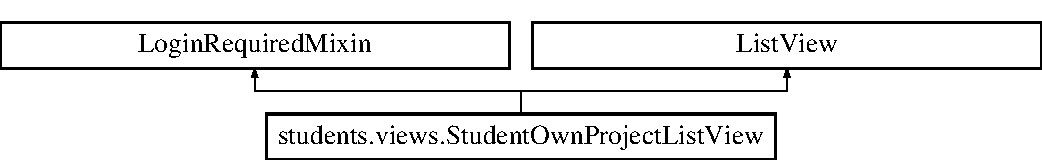
\includegraphics[height=2.000000cm]{classstudents_1_1views_1_1_student_own_project_list_view}
\end{center}
\end{figure}
\subsection*{Public Member Functions}
\begin{DoxyCompactItemize}
\item 
def \hyperlink{classstudents_1_1views_1_1_student_own_project_list_view_a1914d88da030233e5bde8e9eaa672d1f}{dispatch}
\item 
def \hyperlink{classstudents_1_1views_1_1_student_own_project_list_view_a3a005eb9167f0ce90795a497f47192df}{get\-\_\-queryset}
\item 
def \hyperlink{classstudents_1_1views_1_1_student_own_project_list_view_ac4d1e0b97acee38b09e4afa6f19b5183}{get\-\_\-context\-\_\-data}
\end{DoxyCompactItemize}
\subsection*{Static Public Attributes}
\begin{DoxyCompactItemize}
\item 
string \hyperlink{classstudents_1_1views_1_1_student_own_project_list_view_af9ad46ae5b73ff58b70afb6f463dcd28}{template\-\_\-name} = \char`\"{}student\-\_\-own\-\_\-project\-\_\-list\-\_\-view.\-html\char`\"{}
\item 
string \hyperlink{classstudents_1_1views_1_1_student_own_project_list_view_ab68e4688743c572f94ce263b0d25f25c}{login\-\_\-url} = \char`\"{}/students/login/\char`\"{}
\item 
\hyperlink{classstudents_1_1views_1_1_student_own_project_list_view_ab24de360971615cba8e75d65a835ceaf}{model} = Student\-Project
\end{DoxyCompactItemize}


\subsection{Member Function Documentation}
\hypertarget{classstudents_1_1views_1_1_student_own_project_list_view_a1914d88da030233e5bde8e9eaa672d1f}{\index{students\-::views\-::\-Student\-Own\-Project\-List\-View@{students\-::views\-::\-Student\-Own\-Project\-List\-View}!dispatch@{dispatch}}
\index{dispatch@{dispatch}!students::views::StudentOwnProjectListView@{students\-::views\-::\-Student\-Own\-Project\-List\-View}}
\subsubsection[{dispatch}]{\setlength{\rightskip}{0pt plus 5cm}def students.\-views.\-Student\-Own\-Project\-List\-View.\-dispatch (
\begin{DoxyParamCaption}
\item[{}]{self, }
\item[{}]{request, }
\item[{}]{args, }
\item[{}]{kwargs}
\end{DoxyParamCaption}
)}}\label{classstudents_1_1views_1_1_student_own_project_list_view_a1914d88da030233e5bde8e9eaa672d1f}
\hypertarget{classstudents_1_1views_1_1_student_own_project_list_view_ac4d1e0b97acee38b09e4afa6f19b5183}{\index{students\-::views\-::\-Student\-Own\-Project\-List\-View@{students\-::views\-::\-Student\-Own\-Project\-List\-View}!get\-\_\-context\-\_\-data@{get\-\_\-context\-\_\-data}}
\index{get\-\_\-context\-\_\-data@{get\-\_\-context\-\_\-data}!students::views::StudentOwnProjectListView@{students\-::views\-::\-Student\-Own\-Project\-List\-View}}
\subsubsection[{get\-\_\-context\-\_\-data}]{\setlength{\rightskip}{0pt plus 5cm}def students.\-views.\-Student\-Own\-Project\-List\-View.\-get\-\_\-context\-\_\-data (
\begin{DoxyParamCaption}
\item[{}]{self, }
\item[{}]{kwargs}
\end{DoxyParamCaption}
)}}\label{classstudents_1_1views_1_1_student_own_project_list_view_ac4d1e0b97acee38b09e4afa6f19b5183}
\hypertarget{classstudents_1_1views_1_1_student_own_project_list_view_a3a005eb9167f0ce90795a497f47192df}{\index{students\-::views\-::\-Student\-Own\-Project\-List\-View@{students\-::views\-::\-Student\-Own\-Project\-List\-View}!get\-\_\-queryset@{get\-\_\-queryset}}
\index{get\-\_\-queryset@{get\-\_\-queryset}!students::views::StudentOwnProjectListView@{students\-::views\-::\-Student\-Own\-Project\-List\-View}}
\subsubsection[{get\-\_\-queryset}]{\setlength{\rightskip}{0pt plus 5cm}def students.\-views.\-Student\-Own\-Project\-List\-View.\-get\-\_\-queryset (
\begin{DoxyParamCaption}
\item[{}]{self, }
\item[{}]{kwargs}
\end{DoxyParamCaption}
)}}\label{classstudents_1_1views_1_1_student_own_project_list_view_a3a005eb9167f0ce90795a497f47192df}


\subsection{Member Data Documentation}
\hypertarget{classstudents_1_1views_1_1_student_own_project_list_view_ab68e4688743c572f94ce263b0d25f25c}{\index{students\-::views\-::\-Student\-Own\-Project\-List\-View@{students\-::views\-::\-Student\-Own\-Project\-List\-View}!login\-\_\-url@{login\-\_\-url}}
\index{login\-\_\-url@{login\-\_\-url}!students::views::StudentOwnProjectListView@{students\-::views\-::\-Student\-Own\-Project\-List\-View}}
\subsubsection[{login\-\_\-url}]{\setlength{\rightskip}{0pt plus 5cm}string students.\-views.\-Student\-Own\-Project\-List\-View.\-login\-\_\-url = \char`\"{}/students/login/\char`\"{}\hspace{0.3cm}{\ttfamily [static]}}}\label{classstudents_1_1views_1_1_student_own_project_list_view_ab68e4688743c572f94ce263b0d25f25c}
\hypertarget{classstudents_1_1views_1_1_student_own_project_list_view_ab24de360971615cba8e75d65a835ceaf}{\index{students\-::views\-::\-Student\-Own\-Project\-List\-View@{students\-::views\-::\-Student\-Own\-Project\-List\-View}!model@{model}}
\index{model@{model}!students::views::StudentOwnProjectListView@{students\-::views\-::\-Student\-Own\-Project\-List\-View}}
\subsubsection[{model}]{\setlength{\rightskip}{0pt plus 5cm}students.\-views.\-Student\-Own\-Project\-List\-View.\-model = Student\-Project\hspace{0.3cm}{\ttfamily [static]}}}\label{classstudents_1_1views_1_1_student_own_project_list_view_ab24de360971615cba8e75d65a835ceaf}
\hypertarget{classstudents_1_1views_1_1_student_own_project_list_view_af9ad46ae5b73ff58b70afb6f463dcd28}{\index{students\-::views\-::\-Student\-Own\-Project\-List\-View@{students\-::views\-::\-Student\-Own\-Project\-List\-View}!template\-\_\-name@{template\-\_\-name}}
\index{template\-\_\-name@{template\-\_\-name}!students::views::StudentOwnProjectListView@{students\-::views\-::\-Student\-Own\-Project\-List\-View}}
\subsubsection[{template\-\_\-name}]{\setlength{\rightskip}{0pt plus 5cm}string students.\-views.\-Student\-Own\-Project\-List\-View.\-template\-\_\-name = \char`\"{}student\-\_\-own\-\_\-project\-\_\-list\-\_\-view.\-html\char`\"{}\hspace{0.3cm}{\ttfamily [static]}}}\label{classstudents_1_1views_1_1_student_own_project_list_view_af9ad46ae5b73ff58b70afb6f463dcd28}


The documentation for this class was generated from the following file\-:\begin{DoxyCompactItemize}
\item 
leapkit/students/\hyperlink{views_8py}{views.\-py}\end{DoxyCompactItemize}

\hypertarget{classstudents_1_1tests_1_1test__models_1_1_student_profile_test}{\section{students.\-tests.\-test\-\_\-models.\-Student\-Profile\-Test Class Reference}
\label{classstudents_1_1tests_1_1test__models_1_1_student_profile_test}\index{students.\-tests.\-test\-\_\-models.\-Student\-Profile\-Test@{students.\-tests.\-test\-\_\-models.\-Student\-Profile\-Test}}
}
Inheritance diagram for students.\-tests.\-test\-\_\-models.\-Student\-Profile\-Test\-:\begin{figure}[H]
\begin{center}
\leavevmode
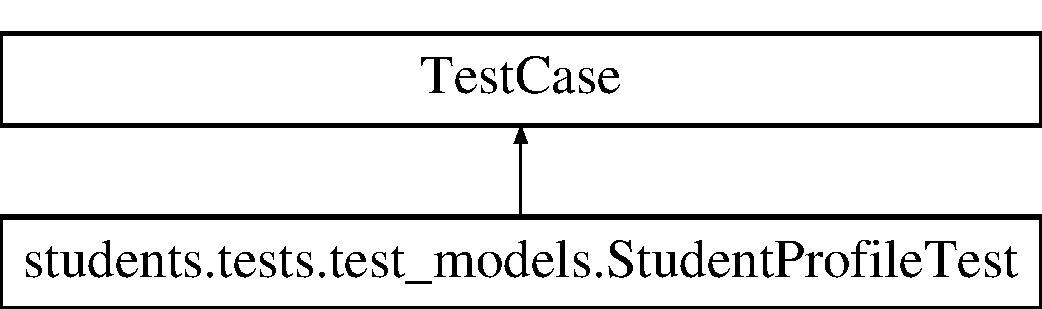
\includegraphics[height=2.000000cm]{classstudents_1_1tests_1_1test__models_1_1_student_profile_test}
\end{center}
\end{figure}
\subsection*{Public Member Functions}
\begin{DoxyCompactItemize}
\item 
def \hyperlink{classstudents_1_1tests_1_1test__models_1_1_student_profile_test_a34c2073c3f3d54023e1cbb35637d5b65}{set\-Up}
\item 
def \hyperlink{classstudents_1_1tests_1_1test__models_1_1_student_profile_test_a86b4cdabc7be80f9e5a9fd4aafb4dc73}{create\-\_\-profile}
\item 
def \hyperlink{classstudents_1_1tests_1_1test__models_1_1_student_profile_test_a2caa47c09a3227ab1dc5a7fe4273045e}{test\-\_\-student\-\_\-profile\-\_\-creation}
\item 
def \hyperlink{classstudents_1_1tests_1_1test__models_1_1_student_profile_test_ac5c9a7314462b9032988018e98b2555c}{test\-\_\-user\-\_\-exists}
\end{DoxyCompactItemize}
\subsection*{Public Attributes}
\begin{DoxyCompactItemize}
\item 
\hyperlink{classstudents_1_1tests_1_1test__models_1_1_student_profile_test_a500cb304853bbf13f8d667f366828573}{user}
\end{DoxyCompactItemize}


\subsection{Member Function Documentation}
\hypertarget{classstudents_1_1tests_1_1test__models_1_1_student_profile_test_a86b4cdabc7be80f9e5a9fd4aafb4dc73}{\index{students\-::tests\-::test\-\_\-models\-::\-Student\-Profile\-Test@{students\-::tests\-::test\-\_\-models\-::\-Student\-Profile\-Test}!create\-\_\-profile@{create\-\_\-profile}}
\index{create\-\_\-profile@{create\-\_\-profile}!students::tests::test_models::StudentProfileTest@{students\-::tests\-::test\-\_\-models\-::\-Student\-Profile\-Test}}
\subsubsection[{create\-\_\-profile}]{\setlength{\rightskip}{0pt plus 5cm}def students.\-tests.\-test\-\_\-models.\-Student\-Profile\-Test.\-create\-\_\-profile (
\begin{DoxyParamCaption}
\item[{}]{self, }
\item[{}]{first\-\_\-name = {\ttfamily \char`\"{}test\char`\"{}}, }
\item[{}]{last\-\_\-name = {\ttfamily \char`\"{}test\char`\"{}}, }
\item[{}]{sex = {\ttfamily \char`\"{}M\char`\"{}}, }
\item[{}]{university = {\ttfamily \char`\"{}ITU\char`\"{}}}
\end{DoxyParamCaption}
)}}\label{classstudents_1_1tests_1_1test__models_1_1_student_profile_test_a86b4cdabc7be80f9e5a9fd4aafb4dc73}
\hypertarget{classstudents_1_1tests_1_1test__models_1_1_student_profile_test_a34c2073c3f3d54023e1cbb35637d5b65}{\index{students\-::tests\-::test\-\_\-models\-::\-Student\-Profile\-Test@{students\-::tests\-::test\-\_\-models\-::\-Student\-Profile\-Test}!set\-Up@{set\-Up}}
\index{set\-Up@{set\-Up}!students::tests::test_models::StudentProfileTest@{students\-::tests\-::test\-\_\-models\-::\-Student\-Profile\-Test}}
\subsubsection[{set\-Up}]{\setlength{\rightskip}{0pt plus 5cm}def students.\-tests.\-test\-\_\-models.\-Student\-Profile\-Test.\-set\-Up (
\begin{DoxyParamCaption}
\item[{}]{self}
\end{DoxyParamCaption}
)}}\label{classstudents_1_1tests_1_1test__models_1_1_student_profile_test_a34c2073c3f3d54023e1cbb35637d5b65}
\hypertarget{classstudents_1_1tests_1_1test__models_1_1_student_profile_test_a2caa47c09a3227ab1dc5a7fe4273045e}{\index{students\-::tests\-::test\-\_\-models\-::\-Student\-Profile\-Test@{students\-::tests\-::test\-\_\-models\-::\-Student\-Profile\-Test}!test\-\_\-student\-\_\-profile\-\_\-creation@{test\-\_\-student\-\_\-profile\-\_\-creation}}
\index{test\-\_\-student\-\_\-profile\-\_\-creation@{test\-\_\-student\-\_\-profile\-\_\-creation}!students::tests::test_models::StudentProfileTest@{students\-::tests\-::test\-\_\-models\-::\-Student\-Profile\-Test}}
\subsubsection[{test\-\_\-student\-\_\-profile\-\_\-creation}]{\setlength{\rightskip}{0pt plus 5cm}def students.\-tests.\-test\-\_\-models.\-Student\-Profile\-Test.\-test\-\_\-student\-\_\-profile\-\_\-creation (
\begin{DoxyParamCaption}
\item[{}]{self}
\end{DoxyParamCaption}
)}}\label{classstudents_1_1tests_1_1test__models_1_1_student_profile_test_a2caa47c09a3227ab1dc5a7fe4273045e}
\hypertarget{classstudents_1_1tests_1_1test__models_1_1_student_profile_test_ac5c9a7314462b9032988018e98b2555c}{\index{students\-::tests\-::test\-\_\-models\-::\-Student\-Profile\-Test@{students\-::tests\-::test\-\_\-models\-::\-Student\-Profile\-Test}!test\-\_\-user\-\_\-exists@{test\-\_\-user\-\_\-exists}}
\index{test\-\_\-user\-\_\-exists@{test\-\_\-user\-\_\-exists}!students::tests::test_models::StudentProfileTest@{students\-::tests\-::test\-\_\-models\-::\-Student\-Profile\-Test}}
\subsubsection[{test\-\_\-user\-\_\-exists}]{\setlength{\rightskip}{0pt plus 5cm}def students.\-tests.\-test\-\_\-models.\-Student\-Profile\-Test.\-test\-\_\-user\-\_\-exists (
\begin{DoxyParamCaption}
\item[{}]{self, }
\item[{}]{profile}
\end{DoxyParamCaption}
)}}\label{classstudents_1_1tests_1_1test__models_1_1_student_profile_test_ac5c9a7314462b9032988018e98b2555c}


\subsection{Member Data Documentation}
\hypertarget{classstudents_1_1tests_1_1test__models_1_1_student_profile_test_a500cb304853bbf13f8d667f366828573}{\index{students\-::tests\-::test\-\_\-models\-::\-Student\-Profile\-Test@{students\-::tests\-::test\-\_\-models\-::\-Student\-Profile\-Test}!user@{user}}
\index{user@{user}!students::tests::test_models::StudentProfileTest@{students\-::tests\-::test\-\_\-models\-::\-Student\-Profile\-Test}}
\subsubsection[{user}]{\setlength{\rightskip}{0pt plus 5cm}students.\-tests.\-test\-\_\-models.\-Student\-Profile\-Test.\-user}}\label{classstudents_1_1tests_1_1test__models_1_1_student_profile_test_a500cb304853bbf13f8d667f366828573}


The documentation for this class was generated from the following file\-:\begin{DoxyCompactItemize}
\item 
leapkit/students/tests/\hyperlink{test__models_8py}{test\-\_\-models.\-py}\end{DoxyCompactItemize}

\hypertarget{classstudents_1_1models_1_1_student_project}{\section{students.\-models.\-Student\-Project Class Reference}
\label{classstudents_1_1models_1_1_student_project}\index{students.\-models.\-Student\-Project@{students.\-models.\-Student\-Project}}
}
Inheritance diagram for students.\-models.\-Student\-Project\-:\begin{figure}[H]
\begin{center}
\leavevmode
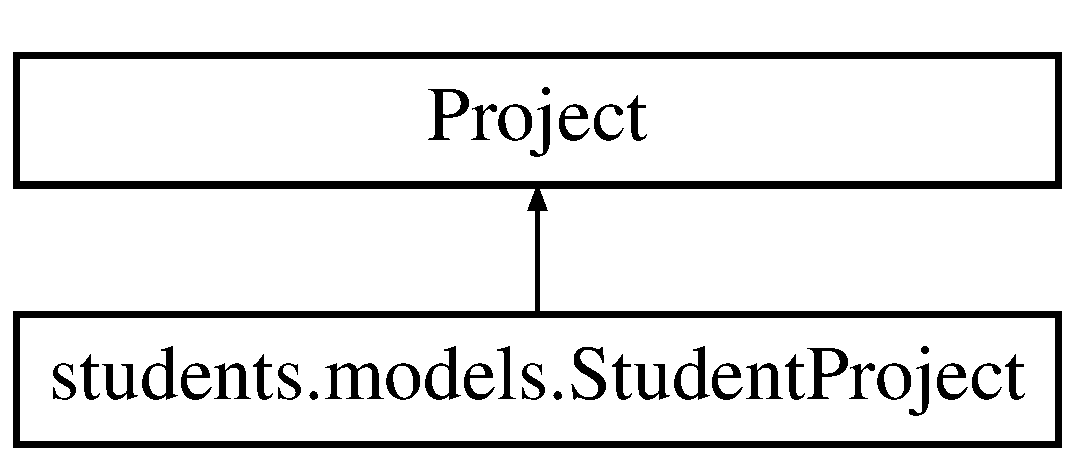
\includegraphics[height=2.000000cm]{classstudents_1_1models_1_1_student_project}
\end{center}
\end{figure}
\subsection*{Static Public Attributes}
\begin{DoxyCompactItemize}
\item 
tuple \hyperlink{classstudents_1_1models_1_1_student_project_a5ba7a623e161f3bc7301273b479c34aa}{project\-\_\-owner} = models.\-Foreign\-Key(\hyperlink{classstudents_1_1models_1_1_student}{Student})
\item 
tuple \hyperlink{classstudents_1_1models_1_1_student_project_ae8b085624144ff16a10d16c43804db51}{objects} = \hyperlink{classstudents_1_1models_1_1_student_project_manager}{Student\-Project\-Manager}()
\end{DoxyCompactItemize}


\subsection{Detailed Description}
\begin{DoxyVerb}This model is to be used for all projects created by companies.
It contains all the fields needed to create an advanced company project.
\end{DoxyVerb}
 

\subsection{Member Data Documentation}
\hypertarget{classstudents_1_1models_1_1_student_project_ae8b085624144ff16a10d16c43804db51}{\index{students\-::models\-::\-Student\-Project@{students\-::models\-::\-Student\-Project}!objects@{objects}}
\index{objects@{objects}!students::models::StudentProject@{students\-::models\-::\-Student\-Project}}
\subsubsection[{objects}]{\setlength{\rightskip}{0pt plus 5cm}tuple students.\-models.\-Student\-Project.\-objects = {\bf Student\-Project\-Manager}()\hspace{0.3cm}{\ttfamily [static]}}}\label{classstudents_1_1models_1_1_student_project_ae8b085624144ff16a10d16c43804db51}
\hypertarget{classstudents_1_1models_1_1_student_project_a5ba7a623e161f3bc7301273b479c34aa}{\index{students\-::models\-::\-Student\-Project@{students\-::models\-::\-Student\-Project}!project\-\_\-owner@{project\-\_\-owner}}
\index{project\-\_\-owner@{project\-\_\-owner}!students::models::StudentProject@{students\-::models\-::\-Student\-Project}}
\subsubsection[{project\-\_\-owner}]{\setlength{\rightskip}{0pt plus 5cm}tuple students.\-models.\-Student\-Project.\-project\-\_\-owner = models.\-Foreign\-Key({\bf Student})\hspace{0.3cm}{\ttfamily [static]}}}\label{classstudents_1_1models_1_1_student_project_a5ba7a623e161f3bc7301273b479c34aa}


The documentation for this class was generated from the following file\-:\begin{DoxyCompactItemize}
\item 
leapkit/students/\hyperlink{models_8py}{models.\-py}\end{DoxyCompactItemize}

\hypertarget{classstudents_1_1admin_1_1_student_project_admin}{\section{students.\-admin.\-Student\-Project\-Admin Class Reference}
\label{classstudents_1_1admin_1_1_student_project_admin}\index{students.\-admin.\-Student\-Project\-Admin@{students.\-admin.\-Student\-Project\-Admin}}
}
Inheritance diagram for students.\-admin.\-Student\-Project\-Admin\-:\begin{figure}[H]
\begin{center}
\leavevmode
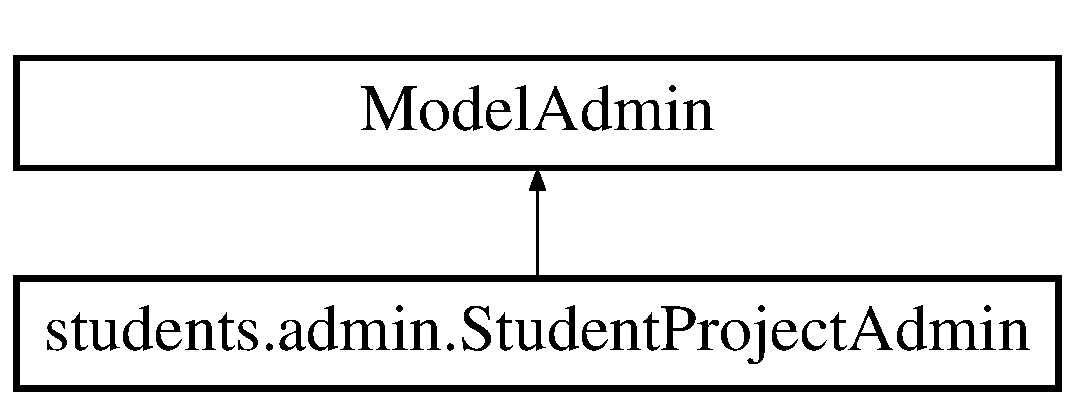
\includegraphics[height=2.000000cm]{classstudents_1_1admin_1_1_student_project_admin}
\end{center}
\end{figure}
\subsection*{Static Public Attributes}
\begin{DoxyCompactItemize}
\item 
list \hyperlink{classstudents_1_1admin_1_1_student_project_admin_ac705b970c858c3a69887299a50844624}{fieldsets}
\item 
tuple \hyperlink{classstudents_1_1admin_1_1_student_project_admin_af38f3f1204fad4b8bdc1b4a7a3e71749}{list\-\_\-display} = ('project\-\_\-owner', 'title', 'contact\-\_\-person', 'contact\-\_\-email', )
\item 
list \hyperlink{classstudents_1_1admin_1_1_student_project_admin_a48716676acc1e54867f4085bec1ae7e7}{search\-\_\-fields} = \mbox{[}'project\-\_\-owner', 'title'\mbox{]}
\item 
list \hyperlink{classstudents_1_1admin_1_1_student_project_admin_a2f15ee6b454237926ee185d9e84afce6}{list\-\_\-filter} = \mbox{[}'contact\-\_\-person', 'open\-\_\-for\-\_\-applications', 'published', 'is\-\_\-active', \mbox{]}
\end{DoxyCompactItemize}


\subsection{Member Data Documentation}
\hypertarget{classstudents_1_1admin_1_1_student_project_admin_ac705b970c858c3a69887299a50844624}{\index{students\-::admin\-::\-Student\-Project\-Admin@{students\-::admin\-::\-Student\-Project\-Admin}!fieldsets@{fieldsets}}
\index{fieldsets@{fieldsets}!students::admin::StudentProjectAdmin@{students\-::admin\-::\-Student\-Project\-Admin}}
\subsubsection[{fieldsets}]{\setlength{\rightskip}{0pt plus 5cm}list students.\-admin.\-Student\-Project\-Admin.\-fieldsets\hspace{0.3cm}{\ttfamily [static]}}}\label{classstudents_1_1admin_1_1_student_project_admin_ac705b970c858c3a69887299a50844624}
{\bfseries Initial value\-:}
\begin{DoxyCode}
1 = [
2         (\textcolor{keywordtype}{None}, \{\textcolor{stringliteral}{'fields'}: [\textcolor{stringliteral}{'project\_owner'},
3                            \textcolor{stringliteral}{'title'},
4                            \textcolor{stringliteral}{'contact\_person'},
5                            \textcolor{stringliteral}{'contact\_email'},
6                            \textcolor{stringliteral}{'contact\_phone'},
7                            \textcolor{stringliteral}{'start\_date'},
8                            \textcolor{stringliteral}{'end\_date'},
9                            \textcolor{stringliteral}{'students\_needed'},
10                            \textcolor{stringliteral}{'short\_description'},
11                            \textcolor{stringliteral}{'full\_description'},
12                            \textcolor{stringliteral}{'project\_document'},
13                            \textcolor{stringliteral}{'published'},
14                            \textcolor{stringliteral}{'project\_type'},
15                            \textcolor{stringliteral}{'education\_requirements'},
16                            \textcolor{stringliteral}{'country\_requirements'},
17                            \textcolor{stringliteral}{'university\_requirements'},
18                            \textcolor{stringliteral}{'related\_lines\_of\_study'},
19                            \textcolor{stringliteral}{'job\_functions'},
20                            \textcolor{stringliteral}{'open\_for\_applications'},
21                            \textcolor{stringliteral}{'is\_active'},
22                            \textcolor{stringliteral}{'views'},
23                            \textcolor{stringliteral}{'detail\_views'}]\}),
24     ]
\end{DoxyCode}
\hypertarget{classstudents_1_1admin_1_1_student_project_admin_af38f3f1204fad4b8bdc1b4a7a3e71749}{\index{students\-::admin\-::\-Student\-Project\-Admin@{students\-::admin\-::\-Student\-Project\-Admin}!list\-\_\-display@{list\-\_\-display}}
\index{list\-\_\-display@{list\-\_\-display}!students::admin::StudentProjectAdmin@{students\-::admin\-::\-Student\-Project\-Admin}}
\subsubsection[{list\-\_\-display}]{\setlength{\rightskip}{0pt plus 5cm}tuple students.\-admin.\-Student\-Project\-Admin.\-list\-\_\-display = ('project\-\_\-owner', 'title', 'contact\-\_\-person', 'contact\-\_\-email', )\hspace{0.3cm}{\ttfamily [static]}}}\label{classstudents_1_1admin_1_1_student_project_admin_af38f3f1204fad4b8bdc1b4a7a3e71749}
\hypertarget{classstudents_1_1admin_1_1_student_project_admin_a2f15ee6b454237926ee185d9e84afce6}{\index{students\-::admin\-::\-Student\-Project\-Admin@{students\-::admin\-::\-Student\-Project\-Admin}!list\-\_\-filter@{list\-\_\-filter}}
\index{list\-\_\-filter@{list\-\_\-filter}!students::admin::StudentProjectAdmin@{students\-::admin\-::\-Student\-Project\-Admin}}
\subsubsection[{list\-\_\-filter}]{\setlength{\rightskip}{0pt plus 5cm}list students.\-admin.\-Student\-Project\-Admin.\-list\-\_\-filter = \mbox{[}'contact\-\_\-person', 'open\-\_\-for\-\_\-applications', 'published', 'is\-\_\-active', \mbox{]}\hspace{0.3cm}{\ttfamily [static]}}}\label{classstudents_1_1admin_1_1_student_project_admin_a2f15ee6b454237926ee185d9e84afce6}
\hypertarget{classstudents_1_1admin_1_1_student_project_admin_a48716676acc1e54867f4085bec1ae7e7}{\index{students\-::admin\-::\-Student\-Project\-Admin@{students\-::admin\-::\-Student\-Project\-Admin}!search\-\_\-fields@{search\-\_\-fields}}
\index{search\-\_\-fields@{search\-\_\-fields}!students::admin::StudentProjectAdmin@{students\-::admin\-::\-Student\-Project\-Admin}}
\subsubsection[{search\-\_\-fields}]{\setlength{\rightskip}{0pt plus 5cm}list students.\-admin.\-Student\-Project\-Admin.\-search\-\_\-fields = \mbox{[}'project\-\_\-owner', 'title'\mbox{]}\hspace{0.3cm}{\ttfamily [static]}}}\label{classstudents_1_1admin_1_1_student_project_admin_a48716676acc1e54867f4085bec1ae7e7}


The documentation for this class was generated from the following file\-:\begin{DoxyCompactItemize}
\item 
leapkit/students/\hyperlink{admin_8py}{admin.\-py}\end{DoxyCompactItemize}

\hypertarget{classstudents_1_1views_1_1_student_project_creation_view}{\section{students.\-views.\-Student\-Project\-Creation\-View Class Reference}
\label{classstudents_1_1views_1_1_student_project_creation_view}\index{students.\-views.\-Student\-Project\-Creation\-View@{students.\-views.\-Student\-Project\-Creation\-View}}
}
Inheritance diagram for students.\-views.\-Student\-Project\-Creation\-View\-:\begin{figure}[H]
\begin{center}
\leavevmode
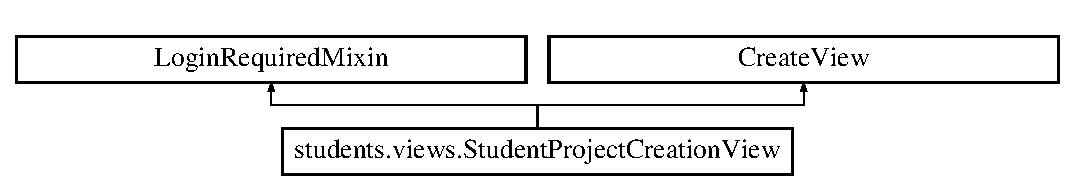
\includegraphics[height=2.000000cm]{classstudents_1_1views_1_1_student_project_creation_view}
\end{center}
\end{figure}
\subsection*{Public Member Functions}
\begin{DoxyCompactItemize}
\item 
def \hyperlink{classstudents_1_1views_1_1_student_project_creation_view_abab72acbf11b726e50eb44f97965430c}{dispatch}
\item 
def \hyperlink{classstudents_1_1views_1_1_student_project_creation_view_a3b2f139feec7b5eb7cc843c85355a4e5}{form\-\_\-valid}
\end{DoxyCompactItemize}
\subsection*{Static Public Attributes}
\begin{DoxyCompactItemize}
\item 
string \hyperlink{classstudents_1_1views_1_1_student_project_creation_view_a07eb488f8065c396ce7de30defb9cfc7}{template\-\_\-name} = \char`\"{}student\-\_\-project\-\_\-creation\-\_\-view.\-html\char`\"{}
\item 
string \hyperlink{classstudents_1_1views_1_1_student_project_creation_view_a4e70c0359cfb38688ba9af46c5e8349d}{login\-\_\-url} = \char`\"{}/students/login/\char`\"{}
\item 
\hyperlink{classstudents_1_1views_1_1_student_project_creation_view_ac30385a37dc52e2e578433f54645844b}{model} = Student\-Project
\item 
\hyperlink{classstudents_1_1views_1_1_student_project_creation_view_a8e507a48d680de20cb41f5d3e608b3e4}{form\-\_\-class} = Student\-Project\-Form
\end{DoxyCompactItemize}


\subsection{Member Function Documentation}
\hypertarget{classstudents_1_1views_1_1_student_project_creation_view_abab72acbf11b726e50eb44f97965430c}{\index{students\-::views\-::\-Student\-Project\-Creation\-View@{students\-::views\-::\-Student\-Project\-Creation\-View}!dispatch@{dispatch}}
\index{dispatch@{dispatch}!students::views::StudentProjectCreationView@{students\-::views\-::\-Student\-Project\-Creation\-View}}
\subsubsection[{dispatch}]{\setlength{\rightskip}{0pt plus 5cm}def students.\-views.\-Student\-Project\-Creation\-View.\-dispatch (
\begin{DoxyParamCaption}
\item[{}]{self, }
\item[{}]{request, }
\item[{}]{args, }
\item[{}]{kwargs}
\end{DoxyParamCaption}
)}}\label{classstudents_1_1views_1_1_student_project_creation_view_abab72acbf11b726e50eb44f97965430c}
\hypertarget{classstudents_1_1views_1_1_student_project_creation_view_a3b2f139feec7b5eb7cc843c85355a4e5}{\index{students\-::views\-::\-Student\-Project\-Creation\-View@{students\-::views\-::\-Student\-Project\-Creation\-View}!form\-\_\-valid@{form\-\_\-valid}}
\index{form\-\_\-valid@{form\-\_\-valid}!students::views::StudentProjectCreationView@{students\-::views\-::\-Student\-Project\-Creation\-View}}
\subsubsection[{form\-\_\-valid}]{\setlength{\rightskip}{0pt plus 5cm}def students.\-views.\-Student\-Project\-Creation\-View.\-form\-\_\-valid (
\begin{DoxyParamCaption}
\item[{}]{self, }
\item[{}]{form}
\end{DoxyParamCaption}
)}}\label{classstudents_1_1views_1_1_student_project_creation_view_a3b2f139feec7b5eb7cc843c85355a4e5}


\subsection{Member Data Documentation}
\hypertarget{classstudents_1_1views_1_1_student_project_creation_view_a8e507a48d680de20cb41f5d3e608b3e4}{\index{students\-::views\-::\-Student\-Project\-Creation\-View@{students\-::views\-::\-Student\-Project\-Creation\-View}!form\-\_\-class@{form\-\_\-class}}
\index{form\-\_\-class@{form\-\_\-class}!students::views::StudentProjectCreationView@{students\-::views\-::\-Student\-Project\-Creation\-View}}
\subsubsection[{form\-\_\-class}]{\setlength{\rightskip}{0pt plus 5cm}students.\-views.\-Student\-Project\-Creation\-View.\-form\-\_\-class = Student\-Project\-Form\hspace{0.3cm}{\ttfamily [static]}}}\label{classstudents_1_1views_1_1_student_project_creation_view_a8e507a48d680de20cb41f5d3e608b3e4}
\hypertarget{classstudents_1_1views_1_1_student_project_creation_view_a4e70c0359cfb38688ba9af46c5e8349d}{\index{students\-::views\-::\-Student\-Project\-Creation\-View@{students\-::views\-::\-Student\-Project\-Creation\-View}!login\-\_\-url@{login\-\_\-url}}
\index{login\-\_\-url@{login\-\_\-url}!students::views::StudentProjectCreationView@{students\-::views\-::\-Student\-Project\-Creation\-View}}
\subsubsection[{login\-\_\-url}]{\setlength{\rightskip}{0pt plus 5cm}string students.\-views.\-Student\-Project\-Creation\-View.\-login\-\_\-url = \char`\"{}/students/login/\char`\"{}\hspace{0.3cm}{\ttfamily [static]}}}\label{classstudents_1_1views_1_1_student_project_creation_view_a4e70c0359cfb38688ba9af46c5e8349d}
\hypertarget{classstudents_1_1views_1_1_student_project_creation_view_ac30385a37dc52e2e578433f54645844b}{\index{students\-::views\-::\-Student\-Project\-Creation\-View@{students\-::views\-::\-Student\-Project\-Creation\-View}!model@{model}}
\index{model@{model}!students::views::StudentProjectCreationView@{students\-::views\-::\-Student\-Project\-Creation\-View}}
\subsubsection[{model}]{\setlength{\rightskip}{0pt plus 5cm}students.\-views.\-Student\-Project\-Creation\-View.\-model = Student\-Project\hspace{0.3cm}{\ttfamily [static]}}}\label{classstudents_1_1views_1_1_student_project_creation_view_ac30385a37dc52e2e578433f54645844b}
\hypertarget{classstudents_1_1views_1_1_student_project_creation_view_a07eb488f8065c396ce7de30defb9cfc7}{\index{students\-::views\-::\-Student\-Project\-Creation\-View@{students\-::views\-::\-Student\-Project\-Creation\-View}!template\-\_\-name@{template\-\_\-name}}
\index{template\-\_\-name@{template\-\_\-name}!students::views::StudentProjectCreationView@{students\-::views\-::\-Student\-Project\-Creation\-View}}
\subsubsection[{template\-\_\-name}]{\setlength{\rightskip}{0pt plus 5cm}string students.\-views.\-Student\-Project\-Creation\-View.\-template\-\_\-name = \char`\"{}student\-\_\-project\-\_\-creation\-\_\-view.\-html\char`\"{}\hspace{0.3cm}{\ttfamily [static]}}}\label{classstudents_1_1views_1_1_student_project_creation_view_a07eb488f8065c396ce7de30defb9cfc7}


The documentation for this class was generated from the following file\-:\begin{DoxyCompactItemize}
\item 
leapkit/students/\hyperlink{views_8py}{views.\-py}\end{DoxyCompactItemize}

\hypertarget{classstudents_1_1views_1_1_student_project_detail_view}{\section{students.\-views.\-Student\-Project\-Detail\-View Class Reference}
\label{classstudents_1_1views_1_1_student_project_detail_view}\index{students.\-views.\-Student\-Project\-Detail\-View@{students.\-views.\-Student\-Project\-Detail\-View}}
}
Inheritance diagram for students.\-views.\-Student\-Project\-Detail\-View\-:\begin{figure}[H]
\begin{center}
\leavevmode
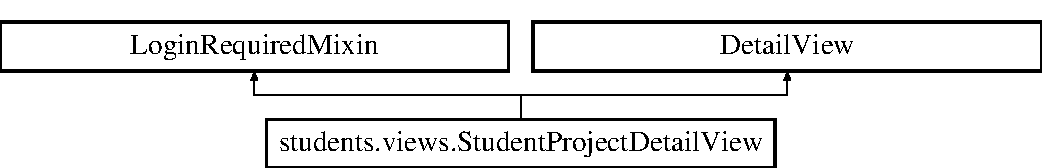
\includegraphics[height=2.000000cm]{classstudents_1_1views_1_1_student_project_detail_view}
\end{center}
\end{figure}
\subsection*{Public Member Functions}
\begin{DoxyCompactItemize}
\item 
def \hyperlink{classstudents_1_1views_1_1_student_project_detail_view_aa6147461550ece1940834db56b32960f}{get\-\_\-queryset}
\end{DoxyCompactItemize}
\subsection*{Static Public Attributes}
\begin{DoxyCompactItemize}
\item 
string \hyperlink{classstudents_1_1views_1_1_student_project_detail_view_a58ec5230c2c0d52ad42510d59e0d647e}{template\-\_\-name} = \char`\"{}student\-\_\-own\-\_\-project\-\_\-detail\-\_\-view.\-html\char`\"{}
\item 
string \hyperlink{classstudents_1_1views_1_1_student_project_detail_view_aa703710c9bb127a1d2ac4e279e329f69}{login\-\_\-url} = \char`\"{}/students/login/\char`\"{}
\item 
\hyperlink{classstudents_1_1views_1_1_student_project_detail_view_a787cda8d76de994a180a8dda8f10e124}{model} = Project
\end{DoxyCompactItemize}


\subsection{Member Function Documentation}
\hypertarget{classstudents_1_1views_1_1_student_project_detail_view_aa6147461550ece1940834db56b32960f}{\index{students\-::views\-::\-Student\-Project\-Detail\-View@{students\-::views\-::\-Student\-Project\-Detail\-View}!get\-\_\-queryset@{get\-\_\-queryset}}
\index{get\-\_\-queryset@{get\-\_\-queryset}!students::views::StudentProjectDetailView@{students\-::views\-::\-Student\-Project\-Detail\-View}}
\subsubsection[{get\-\_\-queryset}]{\setlength{\rightskip}{0pt plus 5cm}def students.\-views.\-Student\-Project\-Detail\-View.\-get\-\_\-queryset (
\begin{DoxyParamCaption}
\item[{}]{self}
\end{DoxyParamCaption}
)}}\label{classstudents_1_1views_1_1_student_project_detail_view_aa6147461550ece1940834db56b32960f}


\subsection{Member Data Documentation}
\hypertarget{classstudents_1_1views_1_1_student_project_detail_view_aa703710c9bb127a1d2ac4e279e329f69}{\index{students\-::views\-::\-Student\-Project\-Detail\-View@{students\-::views\-::\-Student\-Project\-Detail\-View}!login\-\_\-url@{login\-\_\-url}}
\index{login\-\_\-url@{login\-\_\-url}!students::views::StudentProjectDetailView@{students\-::views\-::\-Student\-Project\-Detail\-View}}
\subsubsection[{login\-\_\-url}]{\setlength{\rightskip}{0pt plus 5cm}string students.\-views.\-Student\-Project\-Detail\-View.\-login\-\_\-url = \char`\"{}/students/login/\char`\"{}\hspace{0.3cm}{\ttfamily [static]}}}\label{classstudents_1_1views_1_1_student_project_detail_view_aa703710c9bb127a1d2ac4e279e329f69}
\hypertarget{classstudents_1_1views_1_1_student_project_detail_view_a787cda8d76de994a180a8dda8f10e124}{\index{students\-::views\-::\-Student\-Project\-Detail\-View@{students\-::views\-::\-Student\-Project\-Detail\-View}!model@{model}}
\index{model@{model}!students::views::StudentProjectDetailView@{students\-::views\-::\-Student\-Project\-Detail\-View}}
\subsubsection[{model}]{\setlength{\rightskip}{0pt plus 5cm}students.\-views.\-Student\-Project\-Detail\-View.\-model = Project\hspace{0.3cm}{\ttfamily [static]}}}\label{classstudents_1_1views_1_1_student_project_detail_view_a787cda8d76de994a180a8dda8f10e124}
\hypertarget{classstudents_1_1views_1_1_student_project_detail_view_a58ec5230c2c0d52ad42510d59e0d647e}{\index{students\-::views\-::\-Student\-Project\-Detail\-View@{students\-::views\-::\-Student\-Project\-Detail\-View}!template\-\_\-name@{template\-\_\-name}}
\index{template\-\_\-name@{template\-\_\-name}!students::views::StudentProjectDetailView@{students\-::views\-::\-Student\-Project\-Detail\-View}}
\subsubsection[{template\-\_\-name}]{\setlength{\rightskip}{0pt plus 5cm}string students.\-views.\-Student\-Project\-Detail\-View.\-template\-\_\-name = \char`\"{}student\-\_\-own\-\_\-project\-\_\-detail\-\_\-view.\-html\char`\"{}\hspace{0.3cm}{\ttfamily [static]}}}\label{classstudents_1_1views_1_1_student_project_detail_view_a58ec5230c2c0d52ad42510d59e0d647e}


The documentation for this class was generated from the following file\-:\begin{DoxyCompactItemize}
\item 
leapkit/students/\hyperlink{views_8py}{views.\-py}\end{DoxyCompactItemize}

\hypertarget{classstudents_1_1forms_1_1_student_project_form}{\section{students.\-forms.\-Student\-Project\-Form Class Reference}
\label{classstudents_1_1forms_1_1_student_project_form}\index{students.\-forms.\-Student\-Project\-Form@{students.\-forms.\-Student\-Project\-Form}}
}
Inheritance diagram for students.\-forms.\-Student\-Project\-Form\-:\begin{figure}[H]
\begin{center}
\leavevmode
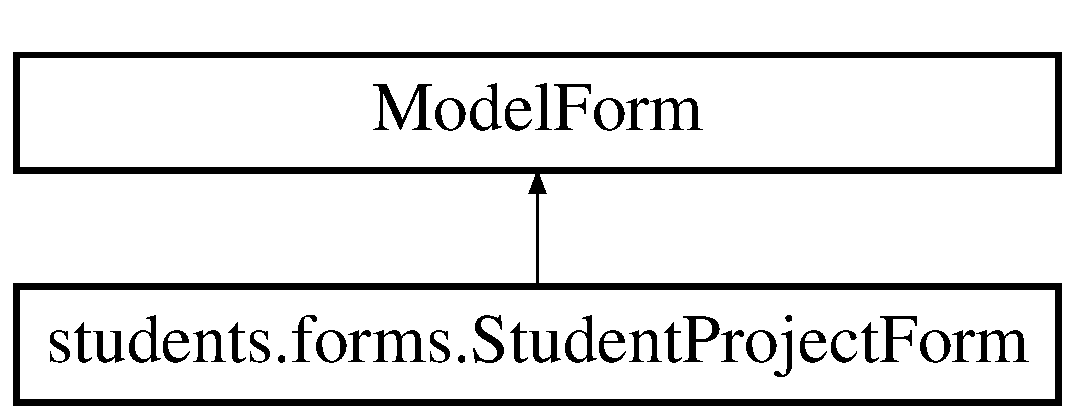
\includegraphics[height=2.000000cm]{classstudents_1_1forms_1_1_student_project_form}
\end{center}
\end{figure}
\subsection*{Classes}
\begin{DoxyCompactItemize}
\item 
class \hyperlink{classstudents_1_1forms_1_1_student_project_form_1_1_meta}{Meta}
\end{DoxyCompactItemize}
\subsection*{Public Member Functions}
\begin{DoxyCompactItemize}
\item 
def \hyperlink{classstudents_1_1forms_1_1_student_project_form_ae9df8bc4e1e2227f05ff0007adfd9e54}{\-\_\-\-\_\-init\-\_\-\-\_\-}
\item 
def \hyperlink{classstudents_1_1forms_1_1_student_project_form_a5458cd762e0b409ec6c796d1b2933f72}{clean\-\_\-students\-\_\-needed}
\item 
def \hyperlink{classstudents_1_1forms_1_1_student_project_form_a84ef8d595a169f889ebd696f9aa0d17e}{clean\-\_\-image}
\end{DoxyCompactItemize}
\subsection*{Public Attributes}
\begin{DoxyCompactItemize}
\item 
\hyperlink{classstudents_1_1forms_1_1_student_project_form_adc6a7a4cceaee86d2cf8370f4993ae99}{helper}
\end{DoxyCompactItemize}
\subsection*{Static Public Attributes}
\begin{DoxyCompactItemize}
\item 
tuple \hyperlink{classstudents_1_1forms_1_1_student_project_form_a6ce0966ef190039162be945d5df7786a}{start\-\_\-date}
\item 
tuple \hyperlink{classstudents_1_1forms_1_1_student_project_form_a14f811fbf8eae30cb9d0b2fd12adcf6b}{end\-\_\-date}
\end{DoxyCompactItemize}


\subsection{Constructor \& Destructor Documentation}
\hypertarget{classstudents_1_1forms_1_1_student_project_form_ae9df8bc4e1e2227f05ff0007adfd9e54}{\index{students\-::forms\-::\-Student\-Project\-Form@{students\-::forms\-::\-Student\-Project\-Form}!\-\_\-\-\_\-init\-\_\-\-\_\-@{\-\_\-\-\_\-init\-\_\-\-\_\-}}
\index{\-\_\-\-\_\-init\-\_\-\-\_\-@{\-\_\-\-\_\-init\-\_\-\-\_\-}!students::forms::StudentProjectForm@{students\-::forms\-::\-Student\-Project\-Form}}
\subsubsection[{\-\_\-\-\_\-init\-\_\-\-\_\-}]{\setlength{\rightskip}{0pt plus 5cm}def students.\-forms.\-Student\-Project\-Form.\-\_\-\-\_\-init\-\_\-\-\_\- (
\begin{DoxyParamCaption}
\item[{}]{self, }
\item[{}]{args, }
\item[{}]{kwargs}
\end{DoxyParamCaption}
)}}\label{classstudents_1_1forms_1_1_student_project_form_ae9df8bc4e1e2227f05ff0007adfd9e54}


\subsection{Member Function Documentation}
\hypertarget{classstudents_1_1forms_1_1_student_project_form_a84ef8d595a169f889ebd696f9aa0d17e}{\index{students\-::forms\-::\-Student\-Project\-Form@{students\-::forms\-::\-Student\-Project\-Form}!clean\-\_\-image@{clean\-\_\-image}}
\index{clean\-\_\-image@{clean\-\_\-image}!students::forms::StudentProjectForm@{students\-::forms\-::\-Student\-Project\-Form}}
\subsubsection[{clean\-\_\-image}]{\setlength{\rightskip}{0pt plus 5cm}def students.\-forms.\-Student\-Project\-Form.\-clean\-\_\-image (
\begin{DoxyParamCaption}
\item[{}]{self}
\end{DoxyParamCaption}
)}}\label{classstudents_1_1forms_1_1_student_project_form_a84ef8d595a169f889ebd696f9aa0d17e}
\hypertarget{classstudents_1_1forms_1_1_student_project_form_a5458cd762e0b409ec6c796d1b2933f72}{\index{students\-::forms\-::\-Student\-Project\-Form@{students\-::forms\-::\-Student\-Project\-Form}!clean\-\_\-students\-\_\-needed@{clean\-\_\-students\-\_\-needed}}
\index{clean\-\_\-students\-\_\-needed@{clean\-\_\-students\-\_\-needed}!students::forms::StudentProjectForm@{students\-::forms\-::\-Student\-Project\-Form}}
\subsubsection[{clean\-\_\-students\-\_\-needed}]{\setlength{\rightskip}{0pt plus 5cm}def students.\-forms.\-Student\-Project\-Form.\-clean\-\_\-students\-\_\-needed (
\begin{DoxyParamCaption}
\item[{}]{self}
\end{DoxyParamCaption}
)}}\label{classstudents_1_1forms_1_1_student_project_form_a5458cd762e0b409ec6c796d1b2933f72}


\subsection{Member Data Documentation}
\hypertarget{classstudents_1_1forms_1_1_student_project_form_a14f811fbf8eae30cb9d0b2fd12adcf6b}{\index{students\-::forms\-::\-Student\-Project\-Form@{students\-::forms\-::\-Student\-Project\-Form}!end\-\_\-date@{end\-\_\-date}}
\index{end\-\_\-date@{end\-\_\-date}!students::forms::StudentProjectForm@{students\-::forms\-::\-Student\-Project\-Form}}
\subsubsection[{end\-\_\-date}]{\setlength{\rightskip}{0pt plus 5cm}tuple students.\-forms.\-Student\-Project\-Form.\-end\-\_\-date\hspace{0.3cm}{\ttfamily [static]}}}\label{classstudents_1_1forms_1_1_student_project_form_a14f811fbf8eae30cb9d0b2fd12adcf6b}
{\bfseries Initial value\-:}
\begin{DoxyCode}
1 = forms.DateField(required=\textcolor{keyword}{False}, help\_text=\textcolor{stringliteral}{"This field is only there if a specific end date"}
2                                                          \textcolor{stringliteral}{" needs to be taken into account"})
\end{DoxyCode}
\hypertarget{classstudents_1_1forms_1_1_student_project_form_adc6a7a4cceaee86d2cf8370f4993ae99}{\index{students\-::forms\-::\-Student\-Project\-Form@{students\-::forms\-::\-Student\-Project\-Form}!helper@{helper}}
\index{helper@{helper}!students::forms::StudentProjectForm@{students\-::forms\-::\-Student\-Project\-Form}}
\subsubsection[{helper}]{\setlength{\rightskip}{0pt plus 5cm}students.\-forms.\-Student\-Project\-Form.\-helper}}\label{classstudents_1_1forms_1_1_student_project_form_adc6a7a4cceaee86d2cf8370f4993ae99}
\hypertarget{classstudents_1_1forms_1_1_student_project_form_a6ce0966ef190039162be945d5df7786a}{\index{students\-::forms\-::\-Student\-Project\-Form@{students\-::forms\-::\-Student\-Project\-Form}!start\-\_\-date@{start\-\_\-date}}
\index{start\-\_\-date@{start\-\_\-date}!students::forms::StudentProjectForm@{students\-::forms\-::\-Student\-Project\-Form}}
\subsubsection[{start\-\_\-date}]{\setlength{\rightskip}{0pt plus 5cm}tuple students.\-forms.\-Student\-Project\-Form.\-start\-\_\-date\hspace{0.3cm}{\ttfamily [static]}}}\label{classstudents_1_1forms_1_1_student_project_form_a6ce0966ef190039162be945d5df7786a}
{\bfseries Initial value\-:}
\begin{DoxyCode}
1 = forms.DateField(required=\textcolor{keyword}{False},
2                                  help\_text=\textcolor{stringliteral}{"This field is only if there is a specific "}
3                                            \textcolor{stringliteral}{"start date that needs to be taken into account"})
\end{DoxyCode}


The documentation for this class was generated from the following file\-:\begin{DoxyCompactItemize}
\item 
leapkit/students/\hyperlink{forms_8py}{forms.\-py}\end{DoxyCompactItemize}

\hypertarget{classstudents_1_1models_1_1_student_project_manager}{\section{students.\-models.\-Student\-Project\-Manager Class Reference}
\label{classstudents_1_1models_1_1_student_project_manager}\index{students.\-models.\-Student\-Project\-Manager@{students.\-models.\-Student\-Project\-Manager}}
}
Inheritance diagram for students.\-models.\-Student\-Project\-Manager\-:\begin{figure}[H]
\begin{center}
\leavevmode
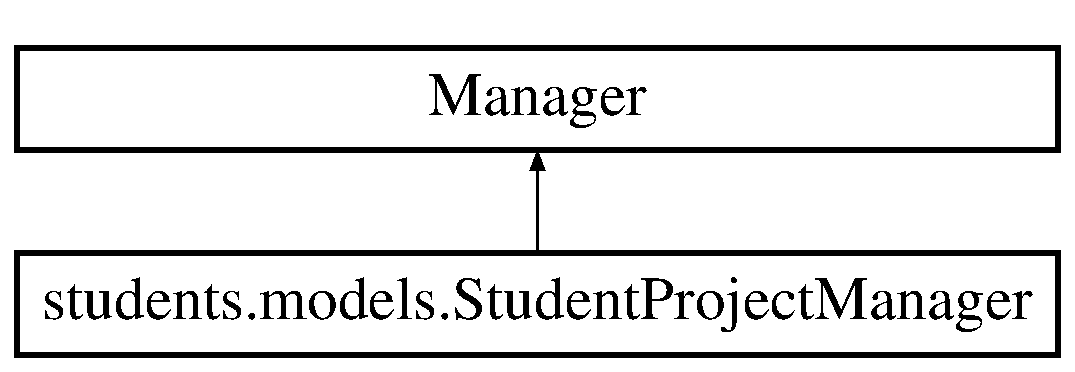
\includegraphics[height=2.000000cm]{classstudents_1_1models_1_1_student_project_manager}
\end{center}
\end{figure}
\subsection*{Public Member Functions}
\begin{DoxyCompactItemize}
\item 
def \hyperlink{classstudents_1_1models_1_1_student_project_manager_ad3c648c438aa4d5843bd6c126c392447}{get\-\_\-own\-\_\-projects}
\item 
def \hyperlink{classstudents_1_1models_1_1_student_project_manager_a03b6388a1e607fe19f5a936cc6413aa7}{get\-\_\-published\-\_\-queryset}
\item 
def \hyperlink{classstudents_1_1models_1_1_student_project_manager_aabfcebd98ffe329aa15c4776dea7ce95}{get\-\_\-own\-\_\-published\-\_\-queryset}
\item 
def \hyperlink{classstudents_1_1models_1_1_student_project_manager_abd14aa2f19159a52589e99a1efbdc28d}{get\-\_\-own\-\_\-drafts\-\_\-queryset}
\end{DoxyCompactItemize}


\subsection{Member Function Documentation}
\hypertarget{classstudents_1_1models_1_1_student_project_manager_abd14aa2f19159a52589e99a1efbdc28d}{\index{students\-::models\-::\-Student\-Project\-Manager@{students\-::models\-::\-Student\-Project\-Manager}!get\-\_\-own\-\_\-drafts\-\_\-queryset@{get\-\_\-own\-\_\-drafts\-\_\-queryset}}
\index{get\-\_\-own\-\_\-drafts\-\_\-queryset@{get\-\_\-own\-\_\-drafts\-\_\-queryset}!students::models::StudentProjectManager@{students\-::models\-::\-Student\-Project\-Manager}}
\subsubsection[{get\-\_\-own\-\_\-drafts\-\_\-queryset}]{\setlength{\rightskip}{0pt plus 5cm}def students.\-models.\-Student\-Project\-Manager.\-get\-\_\-own\-\_\-drafts\-\_\-queryset (
\begin{DoxyParamCaption}
\item[{}]{self, }
\item[{}]{user}
\end{DoxyParamCaption}
)}}\label{classstudents_1_1models_1_1_student_project_manager_abd14aa2f19159a52589e99a1efbdc28d}
\hypertarget{classstudents_1_1models_1_1_student_project_manager_ad3c648c438aa4d5843bd6c126c392447}{\index{students\-::models\-::\-Student\-Project\-Manager@{students\-::models\-::\-Student\-Project\-Manager}!get\-\_\-own\-\_\-projects@{get\-\_\-own\-\_\-projects}}
\index{get\-\_\-own\-\_\-projects@{get\-\_\-own\-\_\-projects}!students::models::StudentProjectManager@{students\-::models\-::\-Student\-Project\-Manager}}
\subsubsection[{get\-\_\-own\-\_\-projects}]{\setlength{\rightskip}{0pt plus 5cm}def students.\-models.\-Student\-Project\-Manager.\-get\-\_\-own\-\_\-projects (
\begin{DoxyParamCaption}
\item[{}]{self, }
\item[{}]{user}
\end{DoxyParamCaption}
)}}\label{classstudents_1_1models_1_1_student_project_manager_ad3c648c438aa4d5843bd6c126c392447}
\hypertarget{classstudents_1_1models_1_1_student_project_manager_aabfcebd98ffe329aa15c4776dea7ce95}{\index{students\-::models\-::\-Student\-Project\-Manager@{students\-::models\-::\-Student\-Project\-Manager}!get\-\_\-own\-\_\-published\-\_\-queryset@{get\-\_\-own\-\_\-published\-\_\-queryset}}
\index{get\-\_\-own\-\_\-published\-\_\-queryset@{get\-\_\-own\-\_\-published\-\_\-queryset}!students::models::StudentProjectManager@{students\-::models\-::\-Student\-Project\-Manager}}
\subsubsection[{get\-\_\-own\-\_\-published\-\_\-queryset}]{\setlength{\rightskip}{0pt plus 5cm}def students.\-models.\-Student\-Project\-Manager.\-get\-\_\-own\-\_\-published\-\_\-queryset (
\begin{DoxyParamCaption}
\item[{}]{self, }
\item[{}]{user}
\end{DoxyParamCaption}
)}}\label{classstudents_1_1models_1_1_student_project_manager_aabfcebd98ffe329aa15c4776dea7ce95}
\hypertarget{classstudents_1_1models_1_1_student_project_manager_a03b6388a1e607fe19f5a936cc6413aa7}{\index{students\-::models\-::\-Student\-Project\-Manager@{students\-::models\-::\-Student\-Project\-Manager}!get\-\_\-published\-\_\-queryset@{get\-\_\-published\-\_\-queryset}}
\index{get\-\_\-published\-\_\-queryset@{get\-\_\-published\-\_\-queryset}!students::models::StudentProjectManager@{students\-::models\-::\-Student\-Project\-Manager}}
\subsubsection[{get\-\_\-published\-\_\-queryset}]{\setlength{\rightskip}{0pt plus 5cm}def students.\-models.\-Student\-Project\-Manager.\-get\-\_\-published\-\_\-queryset (
\begin{DoxyParamCaption}
\item[{}]{self}
\end{DoxyParamCaption}
)}}\label{classstudents_1_1models_1_1_student_project_manager_a03b6388a1e607fe19f5a936cc6413aa7}


The documentation for this class was generated from the following file\-:\begin{DoxyCompactItemize}
\item 
leapkit/students/\hyperlink{models_8py}{models.\-py}\end{DoxyCompactItemize}

\hypertarget{classstudents_1_1views_1_1_student_project_update_view}{\section{students.\-views.\-Student\-Project\-Update\-View Class Reference}
\label{classstudents_1_1views_1_1_student_project_update_view}\index{students.\-views.\-Student\-Project\-Update\-View@{students.\-views.\-Student\-Project\-Update\-View}}
}
Inheritance diagram for students.\-views.\-Student\-Project\-Update\-View\-:\begin{figure}[H]
\begin{center}
\leavevmode
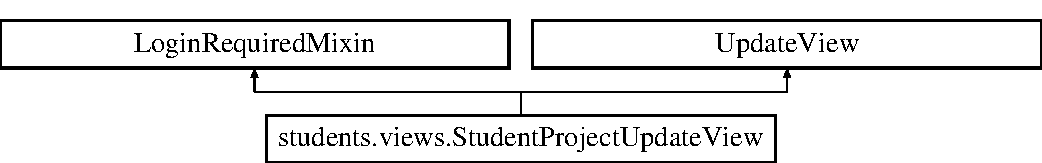
\includegraphics[height=2.000000cm]{classstudents_1_1views_1_1_student_project_update_view}
\end{center}
\end{figure}
\subsection*{Public Member Functions}
\begin{DoxyCompactItemize}
\item 
def \hyperlink{classstudents_1_1views_1_1_student_project_update_view_a6691a76d37261d83f717cfd00103fc26}{form\-\_\-valid}
\end{DoxyCompactItemize}
\subsection*{Static Public Attributes}
\begin{DoxyCompactItemize}
\item 
string \hyperlink{classstudents_1_1views_1_1_student_project_update_view_a7f1c65fd35f5879a287cf60e771c5264}{template\-\_\-name} = \char`\"{}student\-\_\-project\-\_\-update\-\_\-view.\-html\char`\"{}
\item 
string \hyperlink{classstudents_1_1views_1_1_student_project_update_view_af6c8e5b58fd16051dd25dfc3b1607396}{login\-\_\-url} = \char`\"{}/students/login/\char`\"{}
\item 
\hyperlink{classstudents_1_1views_1_1_student_project_update_view_a2a2505466ef2e027d8b58958dca7da67}{model} = Student\-Project
\item 
\hyperlink{classstudents_1_1views_1_1_student_project_update_view_a26de4f28da2fbe3e2c424edb2c791d20}{form\-\_\-class} = Student\-Project\-Form
\end{DoxyCompactItemize}


\subsection{Member Function Documentation}
\hypertarget{classstudents_1_1views_1_1_student_project_update_view_a6691a76d37261d83f717cfd00103fc26}{\index{students\-::views\-::\-Student\-Project\-Update\-View@{students\-::views\-::\-Student\-Project\-Update\-View}!form\-\_\-valid@{form\-\_\-valid}}
\index{form\-\_\-valid@{form\-\_\-valid}!students::views::StudentProjectUpdateView@{students\-::views\-::\-Student\-Project\-Update\-View}}
\subsubsection[{form\-\_\-valid}]{\setlength{\rightskip}{0pt plus 5cm}def students.\-views.\-Student\-Project\-Update\-View.\-form\-\_\-valid (
\begin{DoxyParamCaption}
\item[{}]{self, }
\item[{}]{form}
\end{DoxyParamCaption}
)}}\label{classstudents_1_1views_1_1_student_project_update_view_a6691a76d37261d83f717cfd00103fc26}


\subsection{Member Data Documentation}
\hypertarget{classstudents_1_1views_1_1_student_project_update_view_a26de4f28da2fbe3e2c424edb2c791d20}{\index{students\-::views\-::\-Student\-Project\-Update\-View@{students\-::views\-::\-Student\-Project\-Update\-View}!form\-\_\-class@{form\-\_\-class}}
\index{form\-\_\-class@{form\-\_\-class}!students::views::StudentProjectUpdateView@{students\-::views\-::\-Student\-Project\-Update\-View}}
\subsubsection[{form\-\_\-class}]{\setlength{\rightskip}{0pt plus 5cm}students.\-views.\-Student\-Project\-Update\-View.\-form\-\_\-class = Student\-Project\-Form\hspace{0.3cm}{\ttfamily [static]}}}\label{classstudents_1_1views_1_1_student_project_update_view_a26de4f28da2fbe3e2c424edb2c791d20}
\hypertarget{classstudents_1_1views_1_1_student_project_update_view_af6c8e5b58fd16051dd25dfc3b1607396}{\index{students\-::views\-::\-Student\-Project\-Update\-View@{students\-::views\-::\-Student\-Project\-Update\-View}!login\-\_\-url@{login\-\_\-url}}
\index{login\-\_\-url@{login\-\_\-url}!students::views::StudentProjectUpdateView@{students\-::views\-::\-Student\-Project\-Update\-View}}
\subsubsection[{login\-\_\-url}]{\setlength{\rightskip}{0pt plus 5cm}string students.\-views.\-Student\-Project\-Update\-View.\-login\-\_\-url = \char`\"{}/students/login/\char`\"{}\hspace{0.3cm}{\ttfamily [static]}}}\label{classstudents_1_1views_1_1_student_project_update_view_af6c8e5b58fd16051dd25dfc3b1607396}
\hypertarget{classstudents_1_1views_1_1_student_project_update_view_a2a2505466ef2e027d8b58958dca7da67}{\index{students\-::views\-::\-Student\-Project\-Update\-View@{students\-::views\-::\-Student\-Project\-Update\-View}!model@{model}}
\index{model@{model}!students::views::StudentProjectUpdateView@{students\-::views\-::\-Student\-Project\-Update\-View}}
\subsubsection[{model}]{\setlength{\rightskip}{0pt plus 5cm}students.\-views.\-Student\-Project\-Update\-View.\-model = Student\-Project\hspace{0.3cm}{\ttfamily [static]}}}\label{classstudents_1_1views_1_1_student_project_update_view_a2a2505466ef2e027d8b58958dca7da67}
\hypertarget{classstudents_1_1views_1_1_student_project_update_view_a7f1c65fd35f5879a287cf60e771c5264}{\index{students\-::views\-::\-Student\-Project\-Update\-View@{students\-::views\-::\-Student\-Project\-Update\-View}!template\-\_\-name@{template\-\_\-name}}
\index{template\-\_\-name@{template\-\_\-name}!students::views::StudentProjectUpdateView@{students\-::views\-::\-Student\-Project\-Update\-View}}
\subsubsection[{template\-\_\-name}]{\setlength{\rightskip}{0pt plus 5cm}string students.\-views.\-Student\-Project\-Update\-View.\-template\-\_\-name = \char`\"{}student\-\_\-project\-\_\-update\-\_\-view.\-html\char`\"{}\hspace{0.3cm}{\ttfamily [static]}}}\label{classstudents_1_1views_1_1_student_project_update_view_a7f1c65fd35f5879a287cf60e771c5264}


The documentation for this class was generated from the following file\-:\begin{DoxyCompactItemize}
\item 
leapkit/students/\hyperlink{views_8py}{views.\-py}\end{DoxyCompactItemize}

\hypertarget{classstudents_1_1views_1_1_student_sign_up_view}{\section{students.\-views.\-Student\-Sign\-Up\-View Class Reference}
\label{classstudents_1_1views_1_1_student_sign_up_view}\index{students.\-views.\-Student\-Sign\-Up\-View@{students.\-views.\-Student\-Sign\-Up\-View}}
}
Inheritance diagram for students.\-views.\-Student\-Sign\-Up\-View\-:\begin{figure}[H]
\begin{center}
\leavevmode
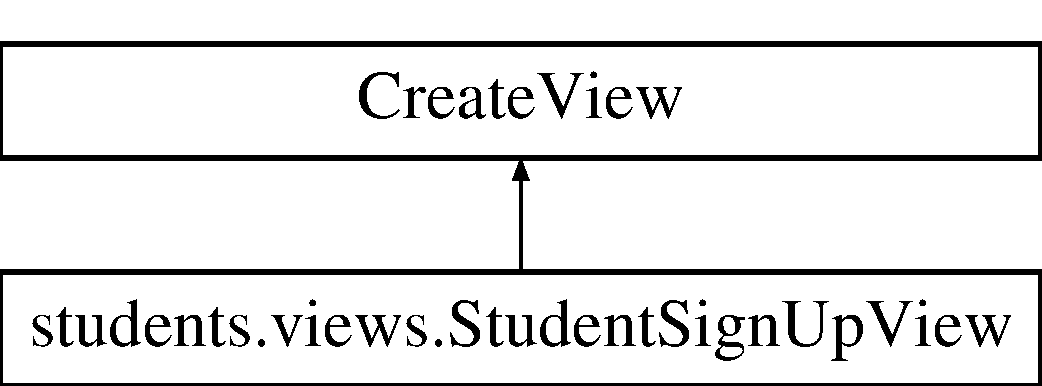
\includegraphics[height=2.000000cm]{classstudents_1_1views_1_1_student_sign_up_view}
\end{center}
\end{figure}
\subsection*{Public Member Functions}
\begin{DoxyCompactItemize}
\item 
def \hyperlink{classstudents_1_1views_1_1_student_sign_up_view_af327972736edd8cd1d9df42c6d44c2a1}{form\-\_\-valid}
\item 
def \hyperlink{classstudents_1_1views_1_1_student_sign_up_view_afbf2ab8d301bfa81d6c9800ad4216667}{form\-\_\-invalid}
\end{DoxyCompactItemize}
\subsection*{Static Public Attributes}
\begin{DoxyCompactItemize}
\item 
string \hyperlink{classstudents_1_1views_1_1_student_sign_up_view_aa49ffb02bfbe89afe87587d289fda4f8}{template\-\_\-name} = \char`\"{}student\-\_\-signup.\-html\char`\"{}
\item 
\hyperlink{classstudents_1_1views_1_1_student_sign_up_view_aebf4f6c965e1539de10429369ec3c8df}{form\-\_\-class} = Student\-Creation\-Form
\item 
\hyperlink{classstudents_1_1views_1_1_student_sign_up_view_a4171ad3e9247829642a13c7047f2b8f1}{model} = Student
\end{DoxyCompactItemize}


\subsection{Member Function Documentation}
\hypertarget{classstudents_1_1views_1_1_student_sign_up_view_afbf2ab8d301bfa81d6c9800ad4216667}{\index{students\-::views\-::\-Student\-Sign\-Up\-View@{students\-::views\-::\-Student\-Sign\-Up\-View}!form\-\_\-invalid@{form\-\_\-invalid}}
\index{form\-\_\-invalid@{form\-\_\-invalid}!students::views::StudentSignUpView@{students\-::views\-::\-Student\-Sign\-Up\-View}}
\subsubsection[{form\-\_\-invalid}]{\setlength{\rightskip}{0pt plus 5cm}def students.\-views.\-Student\-Sign\-Up\-View.\-form\-\_\-invalid (
\begin{DoxyParamCaption}
\item[{}]{self, }
\item[{}]{form}
\end{DoxyParamCaption}
)}}\label{classstudents_1_1views_1_1_student_sign_up_view_afbf2ab8d301bfa81d6c9800ad4216667}
\hypertarget{classstudents_1_1views_1_1_student_sign_up_view_af327972736edd8cd1d9df42c6d44c2a1}{\index{students\-::views\-::\-Student\-Sign\-Up\-View@{students\-::views\-::\-Student\-Sign\-Up\-View}!form\-\_\-valid@{form\-\_\-valid}}
\index{form\-\_\-valid@{form\-\_\-valid}!students::views::StudentSignUpView@{students\-::views\-::\-Student\-Sign\-Up\-View}}
\subsubsection[{form\-\_\-valid}]{\setlength{\rightskip}{0pt plus 5cm}def students.\-views.\-Student\-Sign\-Up\-View.\-form\-\_\-valid (
\begin{DoxyParamCaption}
\item[{}]{self, }
\item[{}]{form}
\end{DoxyParamCaption}
)}}\label{classstudents_1_1views_1_1_student_sign_up_view_af327972736edd8cd1d9df42c6d44c2a1}


\subsection{Member Data Documentation}
\hypertarget{classstudents_1_1views_1_1_student_sign_up_view_aebf4f6c965e1539de10429369ec3c8df}{\index{students\-::views\-::\-Student\-Sign\-Up\-View@{students\-::views\-::\-Student\-Sign\-Up\-View}!form\-\_\-class@{form\-\_\-class}}
\index{form\-\_\-class@{form\-\_\-class}!students::views::StudentSignUpView@{students\-::views\-::\-Student\-Sign\-Up\-View}}
\subsubsection[{form\-\_\-class}]{\setlength{\rightskip}{0pt plus 5cm}students.\-views.\-Student\-Sign\-Up\-View.\-form\-\_\-class = Student\-Creation\-Form\hspace{0.3cm}{\ttfamily [static]}}}\label{classstudents_1_1views_1_1_student_sign_up_view_aebf4f6c965e1539de10429369ec3c8df}
\hypertarget{classstudents_1_1views_1_1_student_sign_up_view_a4171ad3e9247829642a13c7047f2b8f1}{\index{students\-::views\-::\-Student\-Sign\-Up\-View@{students\-::views\-::\-Student\-Sign\-Up\-View}!model@{model}}
\index{model@{model}!students::views::StudentSignUpView@{students\-::views\-::\-Student\-Sign\-Up\-View}}
\subsubsection[{model}]{\setlength{\rightskip}{0pt plus 5cm}students.\-views.\-Student\-Sign\-Up\-View.\-model = Student\hspace{0.3cm}{\ttfamily [static]}}}\label{classstudents_1_1views_1_1_student_sign_up_view_a4171ad3e9247829642a13c7047f2b8f1}
\hypertarget{classstudents_1_1views_1_1_student_sign_up_view_aa49ffb02bfbe89afe87587d289fda4f8}{\index{students\-::views\-::\-Student\-Sign\-Up\-View@{students\-::views\-::\-Student\-Sign\-Up\-View}!template\-\_\-name@{template\-\_\-name}}
\index{template\-\_\-name@{template\-\_\-name}!students::views::StudentSignUpView@{students\-::views\-::\-Student\-Sign\-Up\-View}}
\subsubsection[{template\-\_\-name}]{\setlength{\rightskip}{0pt plus 5cm}string students.\-views.\-Student\-Sign\-Up\-View.\-template\-\_\-name = \char`\"{}student\-\_\-signup.\-html\char`\"{}\hspace{0.3cm}{\ttfamily [static]}}}\label{classstudents_1_1views_1_1_student_sign_up_view_aa49ffb02bfbe89afe87587d289fda4f8}


The documentation for this class was generated from the following file\-:\begin{DoxyCompactItemize}
\item 
leapkit/students/\hyperlink{views_8py}{views.\-py}\end{DoxyCompactItemize}

\hypertarget{classstudents_1_1views_1_1_student_terms_of_usage}{\section{students.\-views.\-Student\-Terms\-Of\-Usage Class Reference}
\label{classstudents_1_1views_1_1_student_terms_of_usage}\index{students.\-views.\-Student\-Terms\-Of\-Usage@{students.\-views.\-Student\-Terms\-Of\-Usage}}
}
Inheritance diagram for students.\-views.\-Student\-Terms\-Of\-Usage\-:\begin{figure}[H]
\begin{center}
\leavevmode
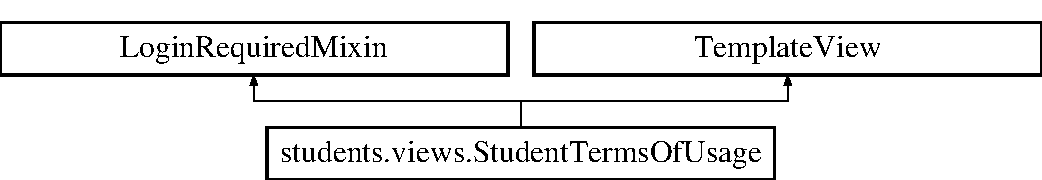
\includegraphics[height=2.000000cm]{classstudents_1_1views_1_1_student_terms_of_usage}
\end{center}
\end{figure}
\subsection*{Static Public Attributes}
\begin{DoxyCompactItemize}
\item 
string \hyperlink{classstudents_1_1views_1_1_student_terms_of_usage_a6dbb8b09152cd323df8fc4a841cb409b}{template\-\_\-name} = \char`\"{}student\-\_\-terms\-\_\-of\-\_\-usage.\-html\char`\"{}
\end{DoxyCompactItemize}


\subsection{Member Data Documentation}
\hypertarget{classstudents_1_1views_1_1_student_terms_of_usage_a6dbb8b09152cd323df8fc4a841cb409b}{\index{students\-::views\-::\-Student\-Terms\-Of\-Usage@{students\-::views\-::\-Student\-Terms\-Of\-Usage}!template\-\_\-name@{template\-\_\-name}}
\index{template\-\_\-name@{template\-\_\-name}!students::views::StudentTermsOfUsage@{students\-::views\-::\-Student\-Terms\-Of\-Usage}}
\subsubsection[{template\-\_\-name}]{\setlength{\rightskip}{0pt plus 5cm}string students.\-views.\-Student\-Terms\-Of\-Usage.\-template\-\_\-name = \char`\"{}student\-\_\-terms\-\_\-of\-\_\-usage.\-html\char`\"{}\hspace{0.3cm}{\ttfamily [static]}}}\label{classstudents_1_1views_1_1_student_terms_of_usage_a6dbb8b09152cd323df8fc4a841cb409b}


The documentation for this class was generated from the following file\-:\begin{DoxyCompactItemize}
\item 
leapkit/students/\hyperlink{views_8py}{views.\-py}\end{DoxyCompactItemize}

\hypertarget{classstudents_1_1views_1_1_student_view}{\section{students.\-views.\-Student\-View Class Reference}
\label{classstudents_1_1views_1_1_student_view}\index{students.\-views.\-Student\-View@{students.\-views.\-Student\-View}}
}
Inheritance diagram for students.\-views.\-Student\-View\-:\begin{figure}[H]
\begin{center}
\leavevmode
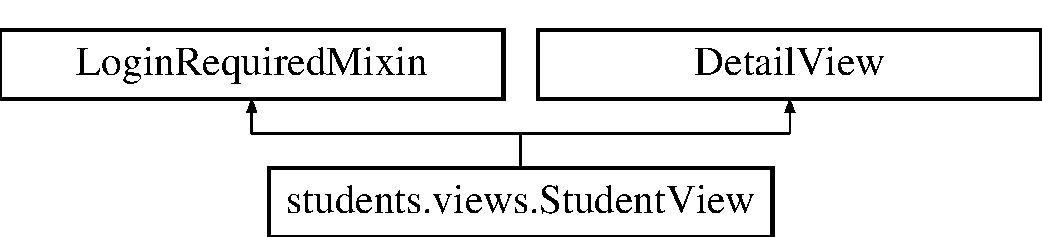
\includegraphics[height=2.000000cm]{classstudents_1_1views_1_1_student_view}
\end{center}
\end{figure}
\subsection*{Public Member Functions}
\begin{DoxyCompactItemize}
\item 
def \hyperlink{classstudents_1_1views_1_1_student_view_ab04c41f2121d32a620fea480ca8dd538}{dispatch}
\item 
def \hyperlink{classstudents_1_1views_1_1_student_view_aea33d4cd9db8ef7b1caf79b8c4502a94}{get\-\_\-context\-\_\-data}
\end{DoxyCompactItemize}
\subsection*{Static Public Attributes}
\begin{DoxyCompactItemize}
\item 
string \hyperlink{classstudents_1_1views_1_1_student_view_aa2e9eac6cab9a9105aa89d3951bbb233}{template\-\_\-name} = \char`\"{}student\-\_\-profile.\-html\char`\"{}
\item 
string \hyperlink{classstudents_1_1views_1_1_student_view_a86ffef39c7d06b2b55d8fdb1f99c19c1}{login\-\_\-url} = \char`\"{}/students/login/\char`\"{}
\item 
\hyperlink{classstudents_1_1views_1_1_student_view_a870052ccf2e29eac0aefd221be2f916b}{model} = Student
\end{DoxyCompactItemize}


\subsection{Member Function Documentation}
\hypertarget{classstudents_1_1views_1_1_student_view_ab04c41f2121d32a620fea480ca8dd538}{\index{students\-::views\-::\-Student\-View@{students\-::views\-::\-Student\-View}!dispatch@{dispatch}}
\index{dispatch@{dispatch}!students::views::StudentView@{students\-::views\-::\-Student\-View}}
\subsubsection[{dispatch}]{\setlength{\rightskip}{0pt plus 5cm}def students.\-views.\-Student\-View.\-dispatch (
\begin{DoxyParamCaption}
\item[{}]{self, }
\item[{}]{request, }
\item[{}]{args, }
\item[{}]{kwargs}
\end{DoxyParamCaption}
)}}\label{classstudents_1_1views_1_1_student_view_ab04c41f2121d32a620fea480ca8dd538}
\hypertarget{classstudents_1_1views_1_1_student_view_aea33d4cd9db8ef7b1caf79b8c4502a94}{\index{students\-::views\-::\-Student\-View@{students\-::views\-::\-Student\-View}!get\-\_\-context\-\_\-data@{get\-\_\-context\-\_\-data}}
\index{get\-\_\-context\-\_\-data@{get\-\_\-context\-\_\-data}!students::views::StudentView@{students\-::views\-::\-Student\-View}}
\subsubsection[{get\-\_\-context\-\_\-data}]{\setlength{\rightskip}{0pt plus 5cm}def students.\-views.\-Student\-View.\-get\-\_\-context\-\_\-data (
\begin{DoxyParamCaption}
\item[{}]{self, }
\item[{}]{kwargs}
\end{DoxyParamCaption}
)}}\label{classstudents_1_1views_1_1_student_view_aea33d4cd9db8ef7b1caf79b8c4502a94}


\subsection{Member Data Documentation}
\hypertarget{classstudents_1_1views_1_1_student_view_a86ffef39c7d06b2b55d8fdb1f99c19c1}{\index{students\-::views\-::\-Student\-View@{students\-::views\-::\-Student\-View}!login\-\_\-url@{login\-\_\-url}}
\index{login\-\_\-url@{login\-\_\-url}!students::views::StudentView@{students\-::views\-::\-Student\-View}}
\subsubsection[{login\-\_\-url}]{\setlength{\rightskip}{0pt plus 5cm}string students.\-views.\-Student\-View.\-login\-\_\-url = \char`\"{}/students/login/\char`\"{}\hspace{0.3cm}{\ttfamily [static]}}}\label{classstudents_1_1views_1_1_student_view_a86ffef39c7d06b2b55d8fdb1f99c19c1}
\hypertarget{classstudents_1_1views_1_1_student_view_a870052ccf2e29eac0aefd221be2f916b}{\index{students\-::views\-::\-Student\-View@{students\-::views\-::\-Student\-View}!model@{model}}
\index{model@{model}!students::views::StudentView@{students\-::views\-::\-Student\-View}}
\subsubsection[{model}]{\setlength{\rightskip}{0pt plus 5cm}students.\-views.\-Student\-View.\-model = Student\hspace{0.3cm}{\ttfamily [static]}}}\label{classstudents_1_1views_1_1_student_view_a870052ccf2e29eac0aefd221be2f916b}
\hypertarget{classstudents_1_1views_1_1_student_view_aa2e9eac6cab9a9105aa89d3951bbb233}{\index{students\-::views\-::\-Student\-View@{students\-::views\-::\-Student\-View}!template\-\_\-name@{template\-\_\-name}}
\index{template\-\_\-name@{template\-\_\-name}!students::views::StudentView@{students\-::views\-::\-Student\-View}}
\subsubsection[{template\-\_\-name}]{\setlength{\rightskip}{0pt plus 5cm}string students.\-views.\-Student\-View.\-template\-\_\-name = \char`\"{}student\-\_\-profile.\-html\char`\"{}\hspace{0.3cm}{\ttfamily [static]}}}\label{classstudents_1_1views_1_1_student_view_aa2e9eac6cab9a9105aa89d3951bbb233}


The documentation for this class was generated from the following file\-:\begin{DoxyCompactItemize}
\item 
leapkit/students/\hyperlink{views_8py}{views.\-py}\end{DoxyCompactItemize}

\hypertarget{classstudents_1_1views_1_1_update_student_profile_view}{\section{students.\-views.\-Update\-Student\-Profile\-View Class Reference}
\label{classstudents_1_1views_1_1_update_student_profile_view}\index{students.\-views.\-Update\-Student\-Profile\-View@{students.\-views.\-Update\-Student\-Profile\-View}}
}
Inheritance diagram for students.\-views.\-Update\-Student\-Profile\-View\-:\begin{figure}[H]
\begin{center}
\leavevmode
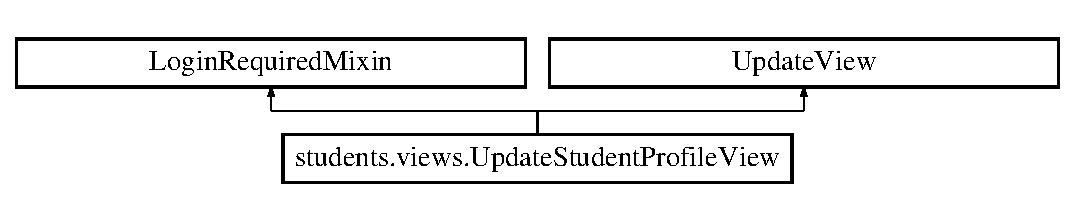
\includegraphics[height=2.000000cm]{classstudents_1_1views_1_1_update_student_profile_view}
\end{center}
\end{figure}
\subsection*{Public Member Functions}
\begin{DoxyCompactItemize}
\item 
def \hyperlink{classstudents_1_1views_1_1_update_student_profile_view_a102eb919b1750833c189b66b1442771b}{form\-\_\-valid}
\item 
def \hyperlink{classstudents_1_1views_1_1_update_student_profile_view_adf9774ac477073f89833c930a725280c}{form\-\_\-invalid}
\end{DoxyCompactItemize}
\subsection*{Static Public Attributes}
\begin{DoxyCompactItemize}
\item 
string \hyperlink{classstudents_1_1views_1_1_update_student_profile_view_a0104ec1afe309e798042732c2b9e4e41}{template\-\_\-name} = \char`\"{}update\-\_\-student\-\_\-profile.\-html\char`\"{}
\item 
string \hyperlink{classstudents_1_1views_1_1_update_student_profile_view_ab788cd36e6f5d47cfab8ee7d911421c6}{login\-\_\-url} = \char`\"{}/students/login/\char`\"{}
\item 
\hyperlink{classstudents_1_1views_1_1_update_student_profile_view_ad150c92fe8f6f8ed6129a2e542c60a5b}{model} = Student
\item 
\hyperlink{classstudents_1_1views_1_1_update_student_profile_view_a0b003ad3198ad35ed33d4c733ceb7f33}{form\-\_\-class} = Student\-Form
\end{DoxyCompactItemize}


\subsection{Member Function Documentation}
\hypertarget{classstudents_1_1views_1_1_update_student_profile_view_adf9774ac477073f89833c930a725280c}{\index{students\-::views\-::\-Update\-Student\-Profile\-View@{students\-::views\-::\-Update\-Student\-Profile\-View}!form\-\_\-invalid@{form\-\_\-invalid}}
\index{form\-\_\-invalid@{form\-\_\-invalid}!students::views::UpdateStudentProfileView@{students\-::views\-::\-Update\-Student\-Profile\-View}}
\subsubsection[{form\-\_\-invalid}]{\setlength{\rightskip}{0pt plus 5cm}def students.\-views.\-Update\-Student\-Profile\-View.\-form\-\_\-invalid (
\begin{DoxyParamCaption}
\item[{}]{self, }
\item[{}]{form}
\end{DoxyParamCaption}
)}}\label{classstudents_1_1views_1_1_update_student_profile_view_adf9774ac477073f89833c930a725280c}
\hypertarget{classstudents_1_1views_1_1_update_student_profile_view_a102eb919b1750833c189b66b1442771b}{\index{students\-::views\-::\-Update\-Student\-Profile\-View@{students\-::views\-::\-Update\-Student\-Profile\-View}!form\-\_\-valid@{form\-\_\-valid}}
\index{form\-\_\-valid@{form\-\_\-valid}!students::views::UpdateStudentProfileView@{students\-::views\-::\-Update\-Student\-Profile\-View}}
\subsubsection[{form\-\_\-valid}]{\setlength{\rightskip}{0pt plus 5cm}def students.\-views.\-Update\-Student\-Profile\-View.\-form\-\_\-valid (
\begin{DoxyParamCaption}
\item[{}]{self, }
\item[{}]{form}
\end{DoxyParamCaption}
)}}\label{classstudents_1_1views_1_1_update_student_profile_view_a102eb919b1750833c189b66b1442771b}


\subsection{Member Data Documentation}
\hypertarget{classstudents_1_1views_1_1_update_student_profile_view_a0b003ad3198ad35ed33d4c733ceb7f33}{\index{students\-::views\-::\-Update\-Student\-Profile\-View@{students\-::views\-::\-Update\-Student\-Profile\-View}!form\-\_\-class@{form\-\_\-class}}
\index{form\-\_\-class@{form\-\_\-class}!students::views::UpdateStudentProfileView@{students\-::views\-::\-Update\-Student\-Profile\-View}}
\subsubsection[{form\-\_\-class}]{\setlength{\rightskip}{0pt plus 5cm}students.\-views.\-Update\-Student\-Profile\-View.\-form\-\_\-class = Student\-Form\hspace{0.3cm}{\ttfamily [static]}}}\label{classstudents_1_1views_1_1_update_student_profile_view_a0b003ad3198ad35ed33d4c733ceb7f33}
\hypertarget{classstudents_1_1views_1_1_update_student_profile_view_ab788cd36e6f5d47cfab8ee7d911421c6}{\index{students\-::views\-::\-Update\-Student\-Profile\-View@{students\-::views\-::\-Update\-Student\-Profile\-View}!login\-\_\-url@{login\-\_\-url}}
\index{login\-\_\-url@{login\-\_\-url}!students::views::UpdateStudentProfileView@{students\-::views\-::\-Update\-Student\-Profile\-View}}
\subsubsection[{login\-\_\-url}]{\setlength{\rightskip}{0pt plus 5cm}string students.\-views.\-Update\-Student\-Profile\-View.\-login\-\_\-url = \char`\"{}/students/login/\char`\"{}\hspace{0.3cm}{\ttfamily [static]}}}\label{classstudents_1_1views_1_1_update_student_profile_view_ab788cd36e6f5d47cfab8ee7d911421c6}
\hypertarget{classstudents_1_1views_1_1_update_student_profile_view_ad150c92fe8f6f8ed6129a2e542c60a5b}{\index{students\-::views\-::\-Update\-Student\-Profile\-View@{students\-::views\-::\-Update\-Student\-Profile\-View}!model@{model}}
\index{model@{model}!students::views::UpdateStudentProfileView@{students\-::views\-::\-Update\-Student\-Profile\-View}}
\subsubsection[{model}]{\setlength{\rightskip}{0pt plus 5cm}students.\-views.\-Update\-Student\-Profile\-View.\-model = Student\hspace{0.3cm}{\ttfamily [static]}}}\label{classstudents_1_1views_1_1_update_student_profile_view_ad150c92fe8f6f8ed6129a2e542c60a5b}
\hypertarget{classstudents_1_1views_1_1_update_student_profile_view_a0104ec1afe309e798042732c2b9e4e41}{\index{students\-::views\-::\-Update\-Student\-Profile\-View@{students\-::views\-::\-Update\-Student\-Profile\-View}!template\-\_\-name@{template\-\_\-name}}
\index{template\-\_\-name@{template\-\_\-name}!students::views::UpdateStudentProfileView@{students\-::views\-::\-Update\-Student\-Profile\-View}}
\subsubsection[{template\-\_\-name}]{\setlength{\rightskip}{0pt plus 5cm}string students.\-views.\-Update\-Student\-Profile\-View.\-template\-\_\-name = \char`\"{}update\-\_\-student\-\_\-profile.\-html\char`\"{}\hspace{0.3cm}{\ttfamily [static]}}}\label{classstudents_1_1views_1_1_update_student_profile_view_a0104ec1afe309e798042732c2b9e4e41}


The documentation for this class was generated from the following file\-:\begin{DoxyCompactItemize}
\item 
leapkit/students/\hyperlink{views_8py}{views.\-py}\end{DoxyCompactItemize}

\chapter{File Documentation}
\hypertarget{____init_____8py}{\section{leapkit/students/\-\_\-\-\_\-init\-\_\-\-\_\-.py File Reference}
\label{____init_____8py}\index{leapkit/students/\-\_\-\-\_\-init\-\_\-\-\_\-.\-py@{leapkit/students/\-\_\-\-\_\-init\-\_\-\-\_\-.\-py}}
}
\subsection*{Namespaces}
\begin{DoxyCompactItemize}
\item 
\hyperlink{namespacestudents}{students}
\end{DoxyCompactItemize}

\hypertarget{migrations_2____init_____8py}{\section{leapkit/students/migrations/\-\_\-\-\_\-init\-\_\-\-\_\-.py File Reference}
\label{migrations_2____init_____8py}\index{leapkit/students/migrations/\-\_\-\-\_\-init\-\_\-\-\_\-.\-py@{leapkit/students/migrations/\-\_\-\-\_\-init\-\_\-\-\_\-.\-py}}
}
\subsection*{Namespaces}
\begin{DoxyCompactItemize}
\item 
\hyperlink{namespacestudents_1_1migrations}{students.\-migrations}
\end{DoxyCompactItemize}

\hypertarget{tests_2____init_____8py}{\section{leapkit/students/tests/\-\_\-\-\_\-init\-\_\-\-\_\-.py File Reference}
\label{tests_2____init_____8py}\index{leapkit/students/tests/\-\_\-\-\_\-init\-\_\-\-\_\-.\-py@{leapkit/students/tests/\-\_\-\-\_\-init\-\_\-\-\_\-.\-py}}
}
\subsection*{Namespaces}
\begin{DoxyCompactItemize}
\item 
\hyperlink{namespacestudents_1_1tests}{students.\-tests}
\end{DoxyCompactItemize}

\hypertarget{admin_8py}{\section{leapkit/students/admin.py File Reference}
\label{admin_8py}\index{leapkit/students/admin.\-py@{leapkit/students/admin.\-py}}
}
\subsection*{Classes}
\begin{DoxyCompactItemize}
\item 
class \hyperlink{classstudents_1_1admin_1_1_linked_in_profile_admin}{students.\-admin.\-Linked\-In\-Profile\-Admin}
\item 
class \hyperlink{classstudents_1_1admin_1_1_skill_admin}{students.\-admin.\-Skill\-Admin}
\item 
class \hyperlink{classstudents_1_1admin_1_1_language_admin}{students.\-admin.\-Language\-Admin}
\item 
class \hyperlink{classstudents_1_1admin_1_1_education_admin}{students.\-admin.\-Education\-Admin}
\item 
class \hyperlink{classstudents_1_1admin_1_1_course_admin}{students.\-admin.\-Course\-Admin}
\item 
class \hyperlink{classstudents_1_1admin_1_1_position_admin}{students.\-admin.\-Position\-Admin}
\item 
class \hyperlink{classstudents_1_1admin_1_1_student_admin}{students.\-admin.\-Student\-Admin}
\item 
class \hyperlink{classstudents_1_1admin_1_1_student_project_admin}{students.\-admin.\-Student\-Project\-Admin}
\end{DoxyCompactItemize}
\subsection*{Namespaces}
\begin{DoxyCompactItemize}
\item 
\hyperlink{namespacestudents_1_1admin}{students.\-admin}
\end{DoxyCompactItemize}

\hypertarget{forms_8py}{\section{leapkit/students/forms.py File Reference}
\label{forms_8py}\index{leapkit/students/forms.\-py@{leapkit/students/forms.\-py}}
}
\subsection*{Classes}
\begin{DoxyCompactItemize}
\item 
class \hyperlink{classstudents_1_1forms_1_1_student_form}{students.\-forms.\-Student\-Form}
\item 
class \hyperlink{classstudents_1_1forms_1_1_student_form_1_1_meta}{students.\-forms.\-Student\-Form.\-Meta}
\item 
class \hyperlink{classstudents_1_1forms_1_1_student_project_form}{students.\-forms.\-Student\-Project\-Form}
\item 
class \hyperlink{classstudents_1_1forms_1_1_student_project_form_1_1_meta}{students.\-forms.\-Student\-Project\-Form.\-Meta}
\item 
class \hyperlink{classstudents_1_1forms_1_1_student_creation_form}{students.\-forms.\-Student\-Creation\-Form}
\item 
class \hyperlink{classstudents_1_1forms_1_1_student_creation_form_1_1_meta}{students.\-forms.\-Student\-Creation\-Form.\-Meta}
\item 
class \hyperlink{classstudents_1_1forms_1_1_student_log_in_form}{students.\-forms.\-Student\-Log\-In\-Form}
\item 
class \hyperlink{classstudents_1_1forms_1_1_student_log_in_form_1_1_meta}{students.\-forms.\-Student\-Log\-In\-Form.\-Meta}
\item 
class \hyperlink{classstudents_1_1forms_1_1_change_user_password}{students.\-forms.\-Change\-User\-Password}
\item 
class \hyperlink{classstudents_1_1forms_1_1_change_user_password_1_1_meta}{students.\-forms.\-Change\-User\-Password.\-Meta}
\item 
class \hyperlink{classstudents_1_1forms_1_1_email_form}{students.\-forms.\-Email\-Form}
\item 
class \hyperlink{classstudents_1_1forms_1_1_email_form_1_1_meta}{students.\-forms.\-Email\-Form.\-Meta}
\end{DoxyCompactItemize}
\subsection*{Namespaces}
\begin{DoxyCompactItemize}
\item 
\hyperlink{namespacestudents_1_1forms}{students.\-forms}
\end{DoxyCompactItemize}

\hypertarget{linkedin__connector_8py}{\section{leapkit/students/linkedin\-\_\-connector.py File Reference}
\label{linkedin__connector_8py}\index{leapkit/students/linkedin\-\_\-connector.\-py@{leapkit/students/linkedin\-\_\-connector.\-py}}
}
\subsection*{Namespaces}
\begin{DoxyCompactItemize}
\item 
\hyperlink{namespacestudents_1_1linkedin__connector}{students.\-linkedin\-\_\-connector}
\end{DoxyCompactItemize}
\subsection*{Functions}
\begin{DoxyCompactItemize}
\item 
def \hyperlink{namespacestudents_1_1linkedin__connector_a441dad30135900c2529bb938b9149d50}{students.\-linkedin\-\_\-connector.\-linkedin\-\_\-get\-\_\-url}
\item 
def \hyperlink{namespacestudents_1_1linkedin__connector_a190a3142ce4291a4238261a1f5abcbc7}{students.\-linkedin\-\_\-connector.\-linkedin\-\_\-extract}
\end{DoxyCompactItemize}
\subsection*{Variables}
\begin{DoxyCompactItemize}
\item 
string \hyperlink{namespacestudents_1_1linkedin__connector_ab7ab81b54306450170bb51f2eb78634c}{students.\-linkedin\-\_\-connector.\-\_\-\-\_\-\-A\-P\-I\-\_\-\-K\-E\-Y} = '75yv7bexwfjovt'
\item 
string \hyperlink{namespacestudents_1_1linkedin__connector_aa15a5de7951fe6f777b1937c042aeefe}{students.\-linkedin\-\_\-connector.\-\_\-\-\_\-\-A\-P\-I\-\_\-\-S\-E\-C\-R\-E\-T} = 'Jz3\-Elg\-F0hj1\-R\-Ajb3'
\item 
string \hyperlink{namespacestudents_1_1linkedin__connector_a6e93c6f0f7a20a83ff1808d3f139f8a5}{students.\-linkedin\-\_\-connector.\-\_\-\-\_\-\-R\-E\-T\-U\-R\-N\-\_\-\-U\-R\-L} = 'http\-://www.\-leapkit.\-com'
\end{DoxyCompactItemize}

\hypertarget{linkedin__converter_8py}{\section{leapkit/students/linkedin\-\_\-converter.py File Reference}
\label{linkedin__converter_8py}\index{leapkit/students/linkedin\-\_\-converter.\-py@{leapkit/students/linkedin\-\_\-converter.\-py}}
}
\subsection*{Classes}
\begin{DoxyCompactItemize}
\item 
class \hyperlink{classstudents_1_1linkedin__converter_1_1_person}{students.\-linkedin\-\_\-converter.\-Person}
\begin{DoxyCompactList}\small\item\em Data Structure \#\#. \end{DoxyCompactList}\item 
class \hyperlink{classstudents_1_1linkedin__converter_1_1_language}{students.\-linkedin\-\_\-converter.\-Language}
\item 
class \hyperlink{classstudents_1_1linkedin__converter_1_1_position}{students.\-linkedin\-\_\-converter.\-Position}
\item 
class \hyperlink{classstudents_1_1linkedin__converter_1_1_course}{students.\-linkedin\-\_\-converter.\-Course}
\item 
class \hyperlink{classstudents_1_1linkedin__converter_1_1_skill}{students.\-linkedin\-\_\-converter.\-Skill}
\item 
class \hyperlink{classstudents_1_1linkedin__converter_1_1_education}{students.\-linkedin\-\_\-converter.\-Education}
\end{DoxyCompactItemize}
\subsection*{Namespaces}
\begin{DoxyCompactItemize}
\item 
\hyperlink{namespacestudents_1_1linkedin__converter}{students.\-linkedin\-\_\-converter}
\end{DoxyCompactItemize}
\subsection*{Functions}
\begin{DoxyCompactItemize}
\item 
def \hyperlink{namespacestudents_1_1linkedin__converter_a5b857dc4a26682e6e4112b430f85d0a1}{students.\-linkedin\-\_\-converter.\-get}
\begin{DoxyCompactList}\small\item\em Helper Functions \#\#. \end{DoxyCompactList}\item 
def \hyperlink{namespacestudents_1_1linkedin__converter_a1b0420a55b9327dbde882ef39ec88c8d}{students.\-linkedin\-\_\-converter.\-get\-Sub}
\item 
def \hyperlink{namespacestudents_1_1linkedin__converter_a508bd54255263358fc9b89c527b0be7f}{students.\-linkedin\-\_\-converter.\-create\-Person}
\item 
def \hyperlink{namespacestudents_1_1linkedin__converter_a16da5f0b1783c410f527a823421de832}{students.\-linkedin\-\_\-converter.\-fill\-Full\-Profile}
\item 
def \hyperlink{namespacestudents_1_1linkedin__converter_a9b47375845c60cee3339c9a402730503}{students.\-linkedin\-\_\-converter.\-create\-Sub}
\item 
def \hyperlink{namespacestudents_1_1linkedin__converter_ae303061c29459c69df3dc09d6b495141}{students.\-linkedin\-\_\-converter.\-format\-Date}
\item 
def \hyperlink{namespacestudents_1_1linkedin__converter_ae8ef886dcffd2847cd908b062a361ed6}{students.\-linkedin\-\_\-converter.\-run}
\begin{DoxyCompactList}\small\item\em A\-P\-I \#\#. \end{DoxyCompactList}\item 
def \hyperlink{namespacestudents_1_1linkedin__converter_acbdadb1c069f1195fab80a95e41fad7e}{students.\-linkedin\-\_\-converter.\-from\-File}
\item 
def \hyperlink{namespacestudents_1_1linkedin__converter_aca1591f6328656541c1fe74ad11067b6}{students.\-linkedin\-\_\-converter.\-from\-String}
\end{DoxyCompactItemize}

\hypertarget{matchmaking_8py}{\section{leapkit/students/matchmaking.py File Reference}
\label{matchmaking_8py}\index{leapkit/students/matchmaking.\-py@{leapkit/students/matchmaking.\-py}}
}
\subsection*{Namespaces}
\begin{DoxyCompactItemize}
\item 
\hyperlink{namespacestudents_1_1matchmaking}{students.\-matchmaking}
\end{DoxyCompactItemize}
\subsection*{Functions}
\begin{DoxyCompactItemize}
\item 
def \hyperlink{namespacestudents_1_1matchmaking_af3e519980cd77aceb9fe2a6843ed0eac}{students.\-matchmaking.\-match\-Lists\-Of\-Strings}
\begin{DoxyCompactList}\small\item\em H\-E\-L\-P\-E\-R M\-E\-T\-H\-O\-D\-S \#\#\#\#\#\#\#\#\#\#\#\#\#\#\#. \end{DoxyCompactList}\item 
def \hyperlink{namespacestudents_1_1matchmaking_a4f0b4f490749d746a5c6c710e65214c6}{students.\-matchmaking.\-strict\-Compare}
\item 
def \hyperlink{namespacestudents_1_1matchmaking_a839ce39a9ca3f80d43e51e190d5bf4a4}{students.\-matchmaking.\-contains\-String\-Compare}
\item 
def \hyperlink{namespacestudents_1_1matchmaking_aa3c57417f509579aa72e905cc90bac71}{students.\-matchmaking.\-compare\-Skills}
\item 
def \hyperlink{namespacestudents_1_1matchmaking_a48857c2224c4e283e8745d574b6ab63d}{students.\-matchmaking.\-compare\-Skills\-Full\-String}
\item 
def \hyperlink{namespacestudents_1_1matchmaking_aac73f2cefa7cada176cc1d3896416edc}{students.\-matchmaking.\-parse\-Skills}
\begin{DoxyCompactList}\small\item\em S\-E\-T\-U\-P M\-E\-T\-H\-O\-D\-S \#\#\#\#\#\#\#\#\#\#\#\#\#\#\#3 Used for testing purposes. \end{DoxyCompactList}\item 
def \hyperlink{namespacestudents_1_1matchmaking_a856d112aa07868c6024c35cd0a90c24c}{students.\-matchmaking.\-load\-Projects}
\item 
def \hyperlink{namespacestudents_1_1matchmaking_aa36aaf3aef1354180f31305846591946}{students.\-matchmaking.\-load\-User}
\item 
def \hyperlink{namespacestudents_1_1matchmaking_a3f28ed62649ae8f076cebb31d838a64a}{students.\-matchmaking.\-print\-Projects}
\end{DoxyCompactItemize}
\subsection*{Variables}
\begin{DoxyCompactItemize}
\item 
tuple \hyperlink{namespacestudents_1_1matchmaking_a10ddf73615b34b61e24d9570a53eadf8}{students.\-matchmaking.\-n} = len(sys.\-argv)
\item 
list \hyperlink{namespacestudents_1_1matchmaking_a3d4ffe9845e7326e75ef529734ac9e91}{students.\-matchmaking.\-path\-User} = sys.\-argv\mbox{[}1\mbox{]}
\item 
tuple \hyperlink{namespacestudents_1_1matchmaking_a53165c9d3c68ba55847f8301028564e3}{students.\-matchmaking.\-user\-Skills} = load\-User(path\-User)
\item 
list \hyperlink{namespacestudents_1_1matchmaking_a96ec4d725826c01b8e22d6115967008b}{students.\-matchmaking.\-path\-Proj} = sys.\-argv\mbox{[}2\mbox{]}
\item 
tuple \hyperlink{namespacestudents_1_1matchmaking_a64150aeb721ef104b626012eacefded6}{students.\-matchmaking.\-projects} = load\-Projects(path\-Proj)
\item 
tuple \hyperlink{namespacestudents_1_1matchmaking_ad6b6e78ce4d795b130413ee857e4ee91}{students.\-matchmaking.\-projects\-Ordered} = compare\-Skills(user\-Skills, projects)
\end{DoxyCompactItemize}

\hypertarget{0001__initial_8py}{\section{leapkit/students/migrations/0001\-\_\-initial.py File Reference}
\label{0001__initial_8py}\index{leapkit/students/migrations/0001\-\_\-initial.\-py@{leapkit/students/migrations/0001\-\_\-initial.\-py}}
}
\subsection*{Classes}
\begin{DoxyCompactItemize}
\item 
class \hyperlink{classstudents_1_1migrations_1_10001__initial_1_1_migration}{students.\-migrations.\-0001\-\_\-initial.\-Migration}
\end{DoxyCompactItemize}
\subsection*{Namespaces}
\begin{DoxyCompactItemize}
\item 
\hyperlink{namespacestudents_1_1migrations_1_10001__initial}{students.\-migrations.\-0001\-\_\-initial}
\end{DoxyCompactItemize}

\hypertarget{0002__auto____add__field__student__cv_8py}{\section{leapkit/students/migrations/0002\-\_\-auto\-\_\-\-\_\-add\-\_\-field\-\_\-student\-\_\-cv.py File Reference}
\label{0002__auto____add__field__student__cv_8py}\index{leapkit/students/migrations/0002\-\_\-auto\-\_\-\-\_\-add\-\_\-field\-\_\-student\-\_\-cv.\-py@{leapkit/students/migrations/0002\-\_\-auto\-\_\-\-\_\-add\-\_\-field\-\_\-student\-\_\-cv.\-py}}
}
\subsection*{Classes}
\begin{DoxyCompactItemize}
\item 
class \hyperlink{classstudents_1_1migrations_1_10002__auto____add__field__student__cv_1_1_migration}{students.\-migrations.\-0002\-\_\-auto\-\_\-\-\_\-add\-\_\-field\-\_\-student\-\_\-cv.\-Migration}
\end{DoxyCompactItemize}
\subsection*{Namespaces}
\begin{DoxyCompactItemize}
\item 
\hyperlink{namespacestudents_1_1migrations_1_10002__auto____add__field__student__cv}{students.\-migrations.\-0002\-\_\-auto\-\_\-\-\_\-add\-\_\-field\-\_\-student\-\_\-cv}
\end{DoxyCompactItemize}

\hypertarget{0003__auto____add__field__student__line__of__study_8py}{\section{leapkit/students/migrations/0003\-\_\-auto\-\_\-\-\_\-add\-\_\-field\-\_\-student\-\_\-line\-\_\-of\-\_\-study.py File Reference}
\label{0003__auto____add__field__student__line__of__study_8py}\index{leapkit/students/migrations/0003\-\_\-auto\-\_\-\-\_\-add\-\_\-field\-\_\-student\-\_\-line\-\_\-of\-\_\-study.\-py@{leapkit/students/migrations/0003\-\_\-auto\-\_\-\-\_\-add\-\_\-field\-\_\-student\-\_\-line\-\_\-of\-\_\-study.\-py}}
}
\subsection*{Classes}
\begin{DoxyCompactItemize}
\item 
class \hyperlink{classstudents_1_1migrations_1_10003__auto____add__field__student__line__of__study_1_1_migration}{students.\-migrations.\-0003\-\_\-auto\-\_\-\-\_\-add\-\_\-field\-\_\-student\-\_\-line\-\_\-of\-\_\-study.\-Migration}
\end{DoxyCompactItemize}
\subsection*{Namespaces}
\begin{DoxyCompactItemize}
\item 
\hyperlink{namespacestudents_1_1migrations_1_10003__auto____add__field__student__line__of__study}{students.\-migrations.\-0003\-\_\-auto\-\_\-\-\_\-add\-\_\-field\-\_\-student\-\_\-line\-\_\-of\-\_\-study}
\end{DoxyCompactItemize}

\hypertarget{0004__auto____add__field__student__education__level_8py}{\section{leapkit/students/migrations/0004\-\_\-auto\-\_\-\-\_\-add\-\_\-field\-\_\-student\-\_\-education\-\_\-level.py File Reference}
\label{0004__auto____add__field__student__education__level_8py}\index{leapkit/students/migrations/0004\-\_\-auto\-\_\-\-\_\-add\-\_\-field\-\_\-student\-\_\-education\-\_\-level.\-py@{leapkit/students/migrations/0004\-\_\-auto\-\_\-\-\_\-add\-\_\-field\-\_\-student\-\_\-education\-\_\-level.\-py}}
}
\subsection*{Classes}
\begin{DoxyCompactItemize}
\item 
class \hyperlink{classstudents_1_1migrations_1_10004__auto____add__field__student__education__level_1_1_migration}{students.\-migrations.\-0004\-\_\-auto\-\_\-\-\_\-add\-\_\-field\-\_\-student\-\_\-education\-\_\-level.\-Migration}
\end{DoxyCompactItemize}
\subsection*{Namespaces}
\begin{DoxyCompactItemize}
\item 
\hyperlink{namespacestudents_1_1migrations_1_10004__auto____add__field__student__education__level}{students.\-migrations.\-0004\-\_\-auto\-\_\-\-\_\-add\-\_\-field\-\_\-student\-\_\-education\-\_\-level}
\end{DoxyCompactItemize}

\hypertarget{0005__auto____add__field__student__times__logged__in_8py}{\section{leapkit/students/migrations/0005\-\_\-auto\-\_\-\-\_\-add\-\_\-field\-\_\-student\-\_\-times\-\_\-logged\-\_\-in.py File Reference}
\label{0005__auto____add__field__student__times__logged__in_8py}\index{leapkit/students/migrations/0005\-\_\-auto\-\_\-\-\_\-add\-\_\-field\-\_\-student\-\_\-times\-\_\-logged\-\_\-in.\-py@{leapkit/students/migrations/0005\-\_\-auto\-\_\-\-\_\-add\-\_\-field\-\_\-student\-\_\-times\-\_\-logged\-\_\-in.\-py}}
}
\subsection*{Classes}
\begin{DoxyCompactItemize}
\item 
class \hyperlink{classstudents_1_1migrations_1_10005__auto____add__field__student__times__logged__in_1_1_migration}{students.\-migrations.\-0005\-\_\-auto\-\_\-\-\_\-add\-\_\-field\-\_\-student\-\_\-times\-\_\-logged\-\_\-in.\-Migration}
\end{DoxyCompactItemize}
\subsection*{Namespaces}
\begin{DoxyCompactItemize}
\item 
\hyperlink{namespacestudents_1_1migrations_1_10005__auto____add__field__student__times__logged__in}{students.\-migrations.\-0005\-\_\-auto\-\_\-\-\_\-add\-\_\-field\-\_\-student\-\_\-times\-\_\-logged\-\_\-in}
\end{DoxyCompactItemize}

\hypertarget{models_8py}{\section{leapkit/students/models.py File Reference}
\label{models_8py}\index{leapkit/students/models.\-py@{leapkit/students/models.\-py}}
}
\subsection*{Classes}
\begin{DoxyCompactItemize}
\item 
class \hyperlink{classstudents_1_1models_1_1_student}{students.\-models.\-Student}
\item 
class \hyperlink{classstudents_1_1models_1_1_student_project_manager}{students.\-models.\-Student\-Project\-Manager}
\item 
class \hyperlink{classstudents_1_1models_1_1_student_project}{students.\-models.\-Student\-Project}
\item 
class \hyperlink{classstudents_1_1models_1_1_linked_in_profile}{students.\-models.\-Linked\-In\-Profile}
\item 
class \hyperlink{classstudents_1_1models_1_1_language}{students.\-models.\-Language}
\item 
class \hyperlink{classstudents_1_1models_1_1_course}{students.\-models.\-Course}
\item 
class \hyperlink{classstudents_1_1models_1_1_skill}{students.\-models.\-Skill}
\item 
class \hyperlink{classstudents_1_1models_1_1_education}{students.\-models.\-Education}
\item 
class \hyperlink{classstudents_1_1models_1_1_position}{students.\-models.\-Position}
\end{DoxyCompactItemize}
\subsection*{Namespaces}
\begin{DoxyCompactItemize}
\item 
\hyperlink{namespacestudents_1_1models}{students.\-models}
\end{DoxyCompactItemize}
\subsection*{Functions}
\begin{DoxyCompactItemize}
\item 
def \hyperlink{namespacestudents_1_1models_aa9c9d7bfb7f8035d5302d6adbaa78be2}{students.\-models.\-get\-\_\-image\-\_\-path}
\item 
def \hyperlink{namespacestudents_1_1models_abcc46854fc7fca904e6449a9dbecb9c1}{students.\-models.\-get\-\_\-file\-\_\-path}
\item 
def \hyperlink{namespacestudents_1_1models_a069689ddea4de552ace8449569b9a997}{students.\-models.\-insert\-Linked\-In\-Profile}
\end{DoxyCompactItemize}

\hypertarget{intro__tour_8js}{\section{leapkit/students/static/students/js/intro\-\_\-tour.js File Reference}
\label{intro__tour_8js}\index{leapkit/students/static/students/js/intro\-\_\-tour.\-js@{leapkit/students/static/students/js/intro\-\_\-tour.\-js}}
}
\subsection*{Functions}
\begin{DoxyCompactItemize}
\item 
document \hyperlink{intro__tour_8js_aa15770c6bf2c5547e869e0d028531f23}{ready} (function()\{var label=\$('label\mbox{[}for=\char`\"{}id\-\_\-title\char`\"{}\mbox{]}');label.\-attr(\char`\"{}data-\/step\char`\"{},\char`\"{}1\char`\"{}) label.\-attr(\char`\"{}data-\/intro\char`\"{},\char`\"{}Fields with a $\ast$ attached to the title are required. These fields must be filled out before uploading the project or saving drafts.\char`\"{});var questionmark=\$('\#id\-\_\-title\-\_\-question');questionmark.\-attr(\char`\"{}data-\/step\char`\"{},\char`\"{}2\char`\"{}) questionmark.\-attr(\char`\"{}data-\/intro\char`\"{},\char`\"{}Each field has a questionmark attached to its title. Hover over it to get help on what to write.\char`\"{});var draft\-\_\-button=\$('\#draft\-\_\-button');draft\-\_\-button.\-attr(\char`\"{}data-\/step\char`\"{},\char`\"{}3\char`\"{}) draft\-\_\-button.\-attr(\char`\"{}data-\/intro\char`\"{},\char`\"{}Click here to save a draft of your project. Remember that you need to fill in the required fields before the draft can be saved. \char`\"{});var publish\-\_\-button=\$('\#publish\-\_\-button');publish\-\_\-button.\-attr(\char`\"{}data-\/step\char`\"{},\char`\"{}4\char`\"{}) publish\-\_\-button.\-attr(\char`\"{}data-\/intro\char`\"{}, 'Click here to publish your project.\-It will now be visible to other student users and contact messages will be forwarded to the email you have entered in\char`\"{}Contact email\char`\"{}.');\})
\end{DoxyCompactItemize}


\subsection{Function Documentation}
\hypertarget{intro__tour_8js_aa15770c6bf2c5547e869e0d028531f23}{\index{intro\-\_\-tour.\-js@{intro\-\_\-tour.\-js}!ready@{ready}}
\index{ready@{ready}!intro_tour.js@{intro\-\_\-tour.\-js}}
\subsubsection[{ready}]{\setlength{\rightskip}{0pt plus 5cm}document ready (
\begin{DoxyParamCaption}
\item[{function()\{var label=\$('label\mbox{[}for=\char`\"{}id\-\_\-title\char`\"{}\mbox{]}');label.\-attr(\char`\"{}data-\/step\char`\"{},\char`\"{}1\char`\"{}) label.\-attr(\char`\"{}data-\/intro\char`\"{},\char`\"{}Fields with a $\ast$ attached to the title are required. These fields must be filled out before uploading the project or saving drafts.\char`\"{});var questionmark=\$('\#id\-\_\-title\-\_\-question');questionmark.\-attr(\char`\"{}data-\/step\char`\"{},\char`\"{}2\char`\"{}) questionmark.\-attr(\char`\"{}data-\/intro\char`\"{},\char`\"{}Each field has a questionmark attached to its title. Hover over it to get help on what to write.\char`\"{});var draft\-\_\-button=\$('\#draft\-\_\-button');draft\-\_\-button.\-attr(\char`\"{}data-\/step\char`\"{},\char`\"{}3\char`\"{}) draft\-\_\-button.\-attr(\char`\"{}data-\/intro\char`\"{},\char`\"{}Click here to save a draft of your project. Remember that you need to fill in the required fields before the draft can be saved. \char`\"{});var publish\-\_\-button=\$('\#publish\-\_\-button');publish\-\_\-button.\-attr(\char`\"{}data-\/step\char`\"{},\char`\"{}4\char`\"{}) publish\-\_\-button.\-attr(\char`\"{}data-\/intro\char`\"{}, 'Click here to publish your project.\-It will now be visible to other student users and contact messages will be forwarded to the email you have entered in\char`\"{}Contact email\char`\"{}.');\}}]{}
\end{DoxyParamCaption}
)}}\label{intro__tour_8js_aa15770c6bf2c5547e869e0d028531f23}

\hypertarget{tasks_8py}{\section{leapkit/students/tasks.py File Reference}
\label{tasks_8py}\index{leapkit/students/tasks.\-py@{leapkit/students/tasks.\-py}}
}
\subsection*{Namespaces}
\begin{DoxyCompactItemize}
\item 
\hyperlink{namespacestudents_1_1tasks}{students.\-tasks}
\end{DoxyCompactItemize}
\subsection*{Functions}
\begin{DoxyCompactItemize}
\item 
def \hyperlink{namespacestudents_1_1tasks_ad6eac1d265bd032ad194a05529922634}{students.\-tasks.\-add}
\item 
def \hyperlink{namespacestudents_1_1tasks_a450c9bee6f3154447de9637ef1ee3305}{students.\-tasks.\-mul}
\item 
def \hyperlink{namespacestudents_1_1tasks_ad38617c8d05d606dffb9a4f1aa083d44}{students.\-tasks.\-xsum}
\end{DoxyCompactItemize}

\hypertarget{test__forms_8py}{\section{leapkit/students/tests/test\-\_\-forms.py File Reference}
\label{test__forms_8py}\index{leapkit/students/tests/test\-\_\-forms.\-py@{leapkit/students/tests/test\-\_\-forms.\-py}}
}
\subsection*{Namespaces}
\begin{DoxyCompactItemize}
\item 
\hyperlink{namespacestudents_1_1tests_1_1test__forms}{students.\-tests.\-test\-\_\-forms}
\end{DoxyCompactItemize}

\hypertarget{test__models_8py}{\section{leapkit/students/tests/test\-\_\-models.py File Reference}
\label{test__models_8py}\index{leapkit/students/tests/test\-\_\-models.\-py@{leapkit/students/tests/test\-\_\-models.\-py}}
}
\subsection*{Classes}
\begin{DoxyCompactItemize}
\item 
class \hyperlink{classstudents_1_1tests_1_1test__models_1_1_student_profile_test}{students.\-tests.\-test\-\_\-models.\-Student\-Profile\-Test}
\end{DoxyCompactItemize}
\subsection*{Namespaces}
\begin{DoxyCompactItemize}
\item 
\hyperlink{namespacestudents_1_1tests_1_1test__models}{students.\-tests.\-test\-\_\-models}
\end{DoxyCompactItemize}

\hypertarget{test__views_8py}{\section{leapkit/students/tests/test\-\_\-views.py File Reference}
\label{test__views_8py}\index{leapkit/students/tests/test\-\_\-views.\-py@{leapkit/students/tests/test\-\_\-views.\-py}}
}
\subsection*{Namespaces}
\begin{DoxyCompactItemize}
\item 
\hyperlink{namespacestudents_1_1tests_1_1test__views}{students.\-tests.\-test\-\_\-views}
\end{DoxyCompactItemize}

\hypertarget{urls_8py}{\section{leapkit/students/urls.py File Reference}
\label{urls_8py}\index{leapkit/students/urls.\-py@{leapkit/students/urls.\-py}}
}
\subsection*{Namespaces}
\begin{DoxyCompactItemize}
\item 
\hyperlink{namespacestudents_1_1urls}{students.\-urls}
\end{DoxyCompactItemize}

\hypertarget{views_8py}{\section{leapkit/students/views.py File Reference}
\label{views_8py}\index{leapkit/students/views.\-py@{leapkit/students/views.\-py}}
}
\subsection*{Classes}
\begin{DoxyCompactItemize}
\item 
class \hyperlink{classstudents_1_1views_1_1_student_view}{students.\-views.\-Student\-View}
\item 
class \hyperlink{classstudents_1_1views_1_1_update_student_profile_view}{students.\-views.\-Update\-Student\-Profile\-View}
\item 
class \hyperlink{classstudents_1_1views_1_1_student_own_project_list_view}{students.\-views.\-Student\-Own\-Project\-List\-View}
\item 
class \hyperlink{classstudents_1_1views_1_1_student_project_update_view}{students.\-views.\-Student\-Project\-Update\-View}
\item 
class \hyperlink{classstudents_1_1views_1_1_student_project_detail_view}{students.\-views.\-Student\-Project\-Detail\-View}
\item 
class \hyperlink{classstudents_1_1views_1_1_student_project_creation_view}{students.\-views.\-Student\-Project\-Creation\-View}
\item 
class \hyperlink{classstudents_1_1views_1_1_list_all_projects_view}{students.\-views.\-List\-All\-Projects\-View}
\item 
class \hyperlink{classstudents_1_1views_1_1_all_project_detail_view}{students.\-views.\-All\-Project\-Detail\-View}
\item 
class \hyperlink{classstudents_1_1views_1_1_student_f_a_q_view}{students.\-views.\-Student\-F\-A\-Q\-View}
\item 
class \hyperlink{classstudents_1_1views_1_1_student_feed_back}{students.\-views.\-Student\-Feed\-Back}
\item 
class \hyperlink{classstudents_1_1views_1_1_student_terms_of_usage}{students.\-views.\-Student\-Terms\-Of\-Usage}
\item 
class \hyperlink{classstudents_1_1views_1_1_send_mail_view}{students.\-views.\-Send\-Mail\-View}
\item 
class \hyperlink{classstudents_1_1views_1_1_student_sign_up_view}{students.\-views.\-Student\-Sign\-Up\-View}
\item 
class \hyperlink{classstudents_1_1views_1_1_student_log_in_view}{students.\-views.\-Student\-Log\-In\-View}
\item 
class \hyperlink{classstudents_1_1views_1_1_change_password_view}{students.\-views.\-Change\-Password\-View}
\end{DoxyCompactItemize}
\subsection*{Namespaces}
\begin{DoxyCompactItemize}
\item 
\hyperlink{namespacestudents_1_1views}{students.\-views}
\end{DoxyCompactItemize}
\subsection*{Functions}
\begin{DoxyCompactItemize}
\item 
def \hyperlink{namespacestudents_1_1views_a021cba8bff39e0d31e6a5357dba3e328}{students.\-views.\-all\-\_\-projects\-\_\-filter}
\item 
def \hyperlink{namespacestudents_1_1views_a6e2dff61ac7220b69daca0a08765fae8}{students.\-views.\-student\-\_\-project\-\_\-delete\-\_\-view}
\item 
def \hyperlink{namespacestudents_1_1views_ae09ce1ee44f9b0abd1d61b02f8292b04}{students.\-views.\-student\-\_\-project\-\_\-alter\-\_\-contact\-\_\-view}
\item 
def \hyperlink{namespacestudents_1_1views_affe8eba083124fd78e3034290bdbf45f}{students.\-views.\-sign\-\_\-out\-\_\-view}
\item 
def \hyperlink{namespacestudents_1_1views_aa7b40de1ab2e0525b5b35e3c0f9e7a59}{students.\-views.\-login\-\_\-check}
\item 
def \hyperlink{namespacestudents_1_1views_a8b7d28a21ff72e17a9e1a234cd57bdc4}{students.\-views.\-student\-\_\-sign\-\_\-up\-\_\-success}
\item 
def \hyperlink{namespacestudents_1_1views_af8444fe95e002a6878c151fb4e34bfd9}{students.\-views.\-linkedin\-\_\-redirect}
\item 
def \hyperlink{namespacestudents_1_1views_a4b54ff72b1f36578d7f24ce2e8e0bcc0}{students.\-views.\-stage}
\end{DoxyCompactItemize}

%--- End generated contents ---

% Index
\newpage
\phantomsection
\addcontentsline{toc}{chapter}{Index}
\printindex

\end{document}
